%
% LICENSE
% You are free to:
%    * Share — copy and redistribute the material in any medium or format
%    * Adapt — remix, transform, and build upon the material
%    * The licensor cannot revoke these freedoms as long as you follow the license terms.
%
% Under the following terms:
%    * Attribution — You must give appropriate credit, provide a link to the license, and indicate if changes were made.
%		  You may do so in any reasonable manner, but not in any way that suggests the licensor endorses you or your use.
%    * NonCommercial — You may not use the material for commercial purposes.
%    * ShareAlike — If you remix, transform, or build upon the material, you must distribute your contributions under the same license as the original.
%    * No additional restrictions — You may not apply legal terms or technological measures that legally restrict others from doing anything the license permits.
% 
% more details: http://creativecommons.org/licenses/by-nc-sa/4.0/
%
% authors:	Fabian Gilson
%			Nicolas Genon
%
% main tex file
%

\documentclass[openright,twoside]{memoir}

%%%%%%%%%%%%%%%%%%%%%%%%%%%%%%%%%%%%%%%%%%%%%%%%%%%%%%%%%%%%%%%%%%%%%%%%%%%%%%%%%%%%%%%%%%%%%%%%

\usepackage{calc,soul,fourier}
\usepackage[table]{xcolor}
\usepackage{tabularx}
\usepackage{multirow}
\usepackage{color}
\usepackage{colortbl}
\usepackage{array}
\usepackage{pdflscape}

\usepackage[utf8]{inputenc}
\usepackage[T1]{fontenc}
\usepackage[english]{babel}

\usepackage[pdftex]{graphicx}
\newsubfloat{figure} % Allow subfloats in figure environment

\usepackage{tikz}
\usetikzlibrary{arrows,automata}

\usepackage[linesnumbered]{algorithm2e}

\usepackage{url}
%\usepackage{fixltx2e}
\usepackage[fleqn]{mathtools}
\usepackage{amssymb}
\usepackage{listings}
\usepackage{epigraph}
%\usepackage{minitoc}
\usepackage{titletoc}
\usepackage{microtype}


%\usepackage{natbib}
\usepackage{cite}
\usepackage{bibentry} \nobibliography* % Allows to print bibtex entries in text

\usepackage{paralist}
\usepackage{enumitem}

\usepackage{longtable}
\usepackage{url}
\usepackage{anyfontsize}
\usepackage[hidelinks]{hyperref}
\usepackage{titlesec}
\usepackage{tabu}
\usepackage{pifont}
% commented by NGE \usepackage{glossaries}
% Load the package with the acronym option
%\usepackage[acronym,nomain]{glossaries}
\usepackage[toc]{glossaries}
\usepackage{atbegshi}

%%%%%%%%%%%%%%%%%%%%%%%%%%%%%%%%%%%%%%%%%%%%%%%%%%%%%%%%%%%%%%%%%%%%%%%%%%%%%%%%%%%%%%%%%%%%%%%%

% document metadata
\hypersetup{
	pdfauthor={Xavier Devroey},
	pdfsubject={},
	pdftitle={Behavioural model-based testing of software product lines},
	pdfkeywords={model-based testing, software product line engineering, software testing},
}

%%%%%%%%%%%%%%%%%%%%%%%%%%%%%%%%%%%%%%%%%%%%%%%%%%%%%%%%%%%%%%%%%%%%%%%%%%%%%%%%%%%%%%%%%%%%%%%%

\pretitle{\begin{center}\Huge\bfseries}
\title{Behavioural model-based testing of software product lines}
\posttitle{\par\vskip1em{\normalfont\normalsize\scshape \par\vfill}\end{center}}
\author{Xavier Devroey}
\predate{\vfill\begin{center}\large}

% for croping
\DisemulatePackage{crop} %to allow package 'crop' instead of emulation by 'memoir'
\setstocksize{297mm}{210mm} %a4 paper as base
\settrimmedsize{240mm}{160mm}{*} %use only 24 x 16 area
\usepackage[driver=none,left=1.8cm,top=2cm,right=2.2cm,bottom=2cm]{geometry} %to allow usage of 'crop'
%\usepackage[cam,a4,center]{crop} %load package 'crop' with cropmark
\usepackage[off,a4,center]{crop} %load package 'crop' without cropmarks
\renewcommand{\baselinestretch}{1.05}

%%  increase page size
%%%\addtolength{\topmargin}{-0.4in}
%%%\addtolength{\textheight}{1.4in}

%% my title page inspired from titleTH from Peter Wilson (available at http://mirror.unl.edu/ctan/info/latex-samples/TitlePages/titlepages.pdf)
\newcommand*{\MyTitlePage}{\begingroup
\thispagestyle{empty}
\raggedleft
\vspace*{\baselineskip}

{\textcolor{myblue}{\HUGE Behavioural model-based testing}}\\[.8\baselineskip]
{\textcolor{myblue}{\HUGE of software product lines}}\\[.5\baselineskip]
{\textcolor{myblue}{\Large }}\\[.1\baselineskip]
\textcolor{myblue}{\rule{\linewidth}{.05cm}}\\[.5\baselineskip]

{\LARGE Xavier Devroey}\\[0.130\textheight]

{\small \textbf{\textit{Jury}}\\ \vspace{.2cm} 
\normalsize Dr. Benoit Baudry\\ \color{mygrey}{\small\textit{Inria, Rennes, France}}\\ \vspace*{.1cm}
\normalcolor\normalsize Prof. Myra B. Cohen\\ \color{mygrey}{\small\textit{University of Nebraska-Lincoln, USA }}\\ \vspace*{.1cm}
\normalcolor\normalsize Prof. Vincent Englebert\\ \color{mygrey}{\small\textit{University of Namur, Belgium}}\\ \vspace*{.1cm}
\normalcolor\normalsize Prof. Patrick Heymans\\ \color{mygrey}{\small\textit{University of Namur, Belgium}}\\ \vspace*{.1cm}
\normalcolor\normalsize Dr. Axel Legay\\ \color{mygrey}{\small\textit{University of Namur, Belgium}}\\ \vspace*{.1cm}
\normalcolor\normalsize Dr. Gilles Perrouin\\ \color{mygrey}{\small\textit{University of Namur, Belgium}}\\ \vspace*{.1cm}
\normalcolor\normalsize Prof. Pierre-Yves Schobbens\\ \color{mygrey}{\small\textit{University of Namur, Belgium}}\vfill}\par
\vspace*{1cm}

{\small A thesis submitted in partial fulfilment of the requirements for the\\degree of Doctor of Philosophy in the subject of Computer Science}\par
\vspace*{.5cm}
{\small Supervised by Prof. Pierre-Yves Schobbens and Prof. Patrick Heymans}\par
\vfill

{\begin{flushleft}
\begin{minipage}[c]{.79\textwidth}
\hfill
\raggedleft\small
\color{mygrey}{University of Namur \\ \vspace*{.5\baselineskip} PReCISE Research Center}
\end{minipage}
\begin{minipage}[c]{.20\textwidth}
\hfill
\includegraphics[width=1.5cm]{./pics/Unamur-FACInformatique.png}
\end{minipage}
\end{flushleft}}
\endgroup}


%% for chapters
\makeatletter
\newlength\dlf@normtxtw
\setlength\dlf@normtxtw{\textwidth}
\def\myhelvetfont{\def\sfdefault{mdput}}
\newsavebox{\feline@chapter}
\newcommand\feline@chapter@marker[1][4cm]{%
\sbox\feline@chapter{%
\resizebox{!}{#1}{\fboxsep=1pt%
\colorbox{myblue}{\color{white}\bfseries\thechapter}%
}}%
\rotatebox{90}{%
\resizebox{%
\heightof{\usebox{\feline@chapter}}+\depthof{\usebox{\feline@chapter}}}%
{!}{\scshape\so\@chapapp}}\quad%
\raisebox{\depthof{\usebox{\feline@chapter}}}{\usebox{\feline@chapter}}%
}
\newcommand\feline@chm[1][4cm]{%
\sbox\feline@chapter{\feline@chapter@marker[#1]}%
\makebox[0pt][l]{% aka \rlap
\makebox[1cm][r]{\usebox\feline@chapter}%
}}
\makechapterstyle{daleif1}{
\renewcommand\chapnamefont{\normalfont\Large\raggedleft\so}
\renewcommand\chaptitlefont{\normalfont\huge\bfseries\scshape}
\renewcommand\chapternamenum{}
\renewcommand\printchaptername{}
\renewcommand\printchapternum{\null\hfill\feline@chm[2.5cm]\par}
\renewcommand\afterchapternum{\par\vskip\midchapskip}
\renewcommand\printchaptertitle[1]{\chaptitlefont\raggedleft ##1\par}
}
\makeatother
\chapterstyle{daleif1}


%% for page headers and footers
\makeheadfootruleprefix{ruled}{\color{myblue}}{\color{myblue}}
\makeheadrule {ruled}{\textwidth}{\normalrulethickness} % header line
\makeoddhead {ruled} {} {} {\small\itshape\rightmark} % put section name in small italic
%\makeevenfoot{ruled}{\small\colorbox{myblue}{\color{white}\thepage}}{}{} 
%\makeoddfoot{ruled}{}{}{\small\colorbox{myblue}{\color{white}\thepage}}
\makeevenfoot{ruled}{\thepage}{}{} 
\makeoddfoot{ruled}{}{}{\thepage}

\makepagestyle{rulednohead}
\makeheadfootruleprefix{rulednohead}{}{\color{myblue}}
%\makeevenfoot{rulednohead}{\small\colorbox{myblue}{\color{white}\thepage}}{}{} 
%\makeoddfoot{rulednohead}{}{}{\small\colorbox{myblue}{\color{white}\thepage}}
\makeevenfoot{rulednohead}{\thepage}{}{} 
\makeoddfoot{rulednohead}{}{}{\thepage}


\makeatletter % because of \@chapapp
\makepsmarks {ruled}{
	\nouppercaseheads
	\createmark {chapter} {both} {shownumber}{\@chapapp\ }{. \ }
	\createmark {section} {right}{shownumber}{} {. \space }
	\createmark {subsection} {right}{shownumber}{} {. \space }
	%\createmark {subsubsection}{right}{shownumber}{} {. \space }
	\createplainmark {toc} {both} {\contentsname}
	\createplainmark {lof} {both} {\listfigurename}
	\createplainmark {lot} {both} {\listtablename}
	\createplainmark {bib} {both} {\bibname}
	\createplainmark {index} {both} {\indexname}
	\createplainmark {glossary} {both} {\glossaryname}
}


\makeatother
\setsecnumdepth{subsection}
\maxtocdepth{subsection}
\pagestyle{ruled}
\aliaspagestyle{chapter}{rulednohead}

% redefine list-related default options
\setlist{nolistsep}
\renewenvironment{description}{%
\begin{itemize}[font=\bfseries\color{myblue}]%
%\addtolength{\leftmargin}{5cm}
\addtolength{\itemindent}{2cm}
%
}
{%
\end{itemize}%
}

% citing style
%\setcitestyle{open={[},close={]},semicolon,aysep={ },yysep={,}}
%\let\cite\citep

% redefine emph
\makeatletter
\DeclareRobustCommand{\em}{%
  \@nomath\em \if b\expandafter\@car\f@series\@nil
  \normalfont \else \bfseries\color{myblue} \fi}
\makeatother


% styling url like href
\urlstyle{same}

% redefine tt family
\renewcommand*\ttdefault{txtt}

% path to graphics
\graphicspath{{./}{pics/}}  

% itemize and enumerate color
\newcommand{\sbt}{\,\begin{picture}(-1,1)(-1,-3)\circle*{4}\end{picture}\ }
\renewcommand{\labelitemi}{${\color{myblue}\sbt}$}
\renewcommand{\labelenumi}{\color{myblue}(\theenumi)}

% in paragraph enumeration style 
\setdefaultenum{(i)}{(a)}{}{}

% colorize subsubsection
\titleformat{\subsubsection}
{\color{myblue}\normalfont\bfseries}
{\color{myblue}\thesection}{}{}

%Listings default configuration
\lstset{float,
showspaces=false,
showtabs=false,
breaklines=true,
showstringspaces=false,
tabsize=2,
basicstyle=\footnotesize,
numbers=left,
xleftmargin=3em,
frame=lines,
framexleftmargin=2.5em,
escapeinside={(*@}{@*)}}

% Define TVL language
\lstdefinelanguage{TVL}{
  morekeywords={root,group,opt,allOf,oneOf,someOf}, % list of keywords
  morecomment=[s]{/*}{*/}, % s is for start and end delimiter
  morestring=[b]" % defines that strings are enclosed in double quotes
}

% redefine a couple of commands for compatibility reason
\renewcommand\textservicemark{\unskip\nobreak\textsuperscript{\scshape{\scriptsize SM}}\allowbreak\thinspace\ignorespaces}

%%%%%%%%%%%%%%%%%%%%%%%%%%%%%%%%%%%%%%%%%%%%%%%%%%%%%%%%%%%%%%%%%%%%%%%%%%%%%%%%%%%%%%%%%%%%%%%%

\newcommand{\todo}[1]{\textcolor{blue}{\textbf{To do: #1}\\}}

% -- New commands --
\newcommand{\eg}{\textit{e.g.,~}}
\newcommand{\Eg}{\textit{E.g.,~}}
\newcommand{\ie}{\textit{i.e.,~}}
\newcommand{\Ie}{\textit{I.e.,~}}
\newcommand{\etal}{\textit{et al.}\xspace}
\newcommand{\etc}{\textit{etc.}\xspace}
\newcommand{\wrt}{\textit{w.r.t.~}}
\newcommand{\cfr}{\textit{cfr.~}}
\newcommand{\Cfr}{\textit{Cfr.~}}
\newcommand{\viz}{\textit{viz.~}}
\newcommand{\aka}{\textit{a.k.a.~}}
\newcommand{\cf}{\textit{cf.~}}
\newcommand{\Cf}{\textit{Cf.~}}

% -- Math elements --
\newcommand{\fts}{\mathit{fts}}
\newcommand{\FTS}{\mathit{FTS}}
\newcommand{\fm}{\mathit{fm}}
\newcommand{\fmm}{\mathit{fmm}}
\newcommand{\lts}{\mathit{lts}}

\newcommand{\trans}{\mathit{trans}}
\newcommand{\Act}{\mathit{Act}}
\newcommand{\CNF}{\mathit{CNF}}

\newcommand{\wProd}{\mathit{prod}}
\newcommand{\wMprod}{\mathit{mprod}}
\newcommand{\wScore}{\mathit{score}}
\newcommand{\wToVisit}{\mathit{toVisit}}
\newcommand{\wPath}{\mathit{path}}
\newcommand{\wSAT}{\mathit{SAT}}
\newcommand{\wCov}{\mathit{cov}}
\newcommand{\wPcov}{\mathit{pcov}}

\newcommand{\wJaccard}{\mathit{jaccard}}
\newcommand{\wHamming}{\mathit{hamming}}
\newcommand{\wDice}{\mathit{dice}}
\newcommand{\wAntidice}{\mathit{antidice}}
\newcommand{\wDiss}{\mathit{diss}}
\newcommand{\wAvg}{\mathit{avg}}

\newcommand{\wCurrent}{\mathit{current}}
\newcommand{\wPrevious}{\mathit{previous}}
\newcommand{\wCost}{\mathit{cost}}
\newcommand{\wCandidate}{\mathit{candidate}}
\newcommand{\wRandom}{\mathit{random}}
\newcommand{\wNext}{\mathit{next}}
\newcommand{\wCopy}{\mathit{copy}}

\newcommand{\wTrace}{\mathit{trace}}
\newcommand{\wTraces}{\mathit{traces}}
\newcommand{\wTransitions}{\mathit{transitions}}
\newcommand{\wTransition}{\mathit{transition}}
\newcommand{\wStates}{\mathit{states}}
\newcommand{\wState}{\mathit{state}}
\newcommand{\wFLabels}{\mathit{fLabels}}

\newcommand{\wPr}{\mathit{Pr}}

\newcommand{\sem}{\ensuremath{[\![}}
\newcommand{\mes}{\ensuremath{]\!]}}

\newcommand{\Sem}[1]{\sem#1\mes}


%-- Math theorems --
\newtheorem{definition}{Definition}
\newtheorem{property}{Property}

%%%%%%%%%%%%%%%%%%%%%%%%%%%%%%%%%%%%%%%%%%%%%%%%%%%%%%%%%%%%%%%%%%%%%%%%%%%%%%%%%%%%%%%%%%%%%%%%

\hyphenation{tran-si-tion serve-Soda serve-Tea Tran-sit-ion-Sys-tem Abs-tract-Tran-si-tion-Sys-tem Tran-si-tion-Sys-tem-Ele-ment Fea-tu-red-Tran-si-tion Usa-ge-Mo-del-Tran-si-tion Label-led-Tran-sition-System Fea-tu-red-Tran-sit-ion-System Usage-Mo-del Ab-stract-Tran-si-tion-System Tran-si-tion-Sys-tem-Ele-ment-Facto-ry Fea-tu-red-Tran-si-tion-Sy-stem-De-fi-ni-tion Test-Set-De-fi-ni-tion Schob-bens}

%%%%%%%%%%%%%%%%%%%%%%%%%%%%%%%%%%%%%%%%%%%%%%%%%%%%%%%%%%%%%%%%%%%%%%%%%%%%%%%%%%%%%%%%%%%%%%%%


\makeglossaries

%%  custom  macros %%
%
% LICENSE
% You are free to:
%    * Share — copy and redistribute the material in any medium or format
%    * Adapt — remix, transform, and build upon the material
%    * The licensor cannot revoke these freedoms as long as you follow the license terms.
%
% Under the following terms:
%    * Attribution — You must give appropriate credit, provide a link to the license, and indicate if changes were made.
%		  You may do so in any reasonable manner, but not in any way that suggests the licensor endorses you or your use.
%    * NonCommercial — You may not use the material for commercial purposes.
%    * ShareAlike — If you remix, transform, or build upon the material, you must distribute your contributions under the same license as the original.
%    * No additional restrictions — You may not apply legal terms or technological measures that legally restrict others from doing anything the license permits.
% 
% more details: http://creativecommons.org/licenses/by-nc-sa/4.0/
%
% authors: Fabian Gilson
%					Nicolas Genon
%
% custom latex color macro file
%

\usepackage{xcolor}


% custom colors for source code
\definecolor{codeblue}{HTML}{004385}
\definecolor{codegrey}{HTML}{4D4D4D}
\definecolor{codegreen}{HTML}{518D71}
\definecolor{codeviolet}{HTML}{7F0055}

% 
\definecolor{rulerline}{HTML}{A0A2AC}

% NGE custom colors
\definecolor{mybluetable}{HTML}{63CCFF}
\definecolor{myredtable}{HTML}{FF6666}
\definecolor{mygreentable}{HTML}{33FF99}
\definecolor{myyellowtable}{HTML}{FFFF99}
\definecolor{mylightbluetable}{HTML}{D0F0FF}
\definecolor{mylightredtable}{HTML}{FFD1D1}
\definecolor{mylightgreentable}{HTML}{ADFFD6}
\definecolor{mylightyellowtable}{HTML}{FFFFCC}
\definecolor{mydarkblue}{HTML}{000099}
\definecolor{myred}{HTML}{BC1818}
%\definecolor{mygreen}{HTML}{318731}
\definecolor{mygreen}{HTML}{69be28} % UNamur green
\definecolor{myviolet}{HTML}{8E0630}
%\definecolor{myblue}{HTML}{406E86}
\definecolor{myblue}{HTML}{003366} % Fac Info blue
%\definecolor{myblue2}{HTML}{0D3042}
%\definecolor{mygrey}{HTML}{4D4D4D}
\definecolor{mygrey}{HTML}{616365} % UNamur grey
\definecolor{myyellow}{HTML}{FFFF66}
%\definecolor{mylightgray}{rgb}{.95,.95,.95}
\definecolor{mylightgray}{rgb}{.91,.96,.100} % UNamur light grey

% STC colors
\definecolor{StronglyPerverse}{rgb}{1.0,0.0,0.0}
\definecolor{ModeratelyPerverse}{rgb}{1.0,0.5,0.5}
\definecolor{SlightlyPerverse}{rgb}{1.0,0.86,0.86}
\definecolor{Opaque}{rgb}{1.0,1.0,1.0}
\definecolor{SlightlyTransparent}{rgb}{0.8,1.0,0.8}
\definecolor{ModeratelyTransparent}{rgb}{0.69,1.0,0.64}
\definecolor{StronglyTransparent}{rgb}{0.19,0.72,0.20}
\definecolor{GreenTextColor}{rgb}{0.19,0.72,0.20}

%  user-defined custom colors
\definecolor{lightgray}{rgb}{.9,.9,.9}
\definecolor{darkgray}{rgb}{.4,.4,.4}
\definecolor{purple}{rgb}{0.65, 0.12, 0.82}
\definecolor{Gray}{gray}{0.9}
\definecolor{lightblue}{rgb}{0.46,0.77,0.86}
\definecolor{darkblue}{HTML}{08088A}


%%
% LICENSE
% You are free to:
%    * Share — copy and redistribute the material in any medium or format
%    * Adapt — remix, transform, and build upon the material
%    * The licensor cannot revoke these freedoms as long as you follow the license terms.
%
% Under the following terms:
%    * Attribution — You must give appropriate credit, provide a link to the license, and indicate if changes were made.
%		  You may do so in any reasonable manner, but not in any way that suggests the licensor endorses you or your use.
%    * NonCommercial — You may not use the material for commercial purposes.
%    * ShareAlike — If you remix, transform, or build upon the material, you must distribute your contributions under the same license as the original.
%    * No additional restrictions — You may not apply legal terms or technological measures that legally restrict others from doing anything the license permits.
% 
% more details: http://creativecommons.org/licenses/by-nc-sa/4.0/
% 
% authors: Fabian Gilson
%					Nicolas Genon
%
% custom latex color command macro file
%

%
% TODO command customization
%
\newcommand{\TODO}[1]{\textcolor{blue}{\textbf{TODO~\textit{#1}}}}
% or
\newcommand{\todo}[1]{\textcolor{red}{\textit{\textbf{TODO} : #1}}}

% suppress TODOs 
%\newcommand{\todo}[1]{}



%
% bullets, descriptions, etc
%
\let\descriptionlabel\relax
\newcommand*\descriptionlabel[1]{\hspace\labelsep \normalfont\bfseries #1}

\newlength{\Oldarrayrulewidth}
\newcommand{\Cline}[2]{%
  \noalign{\global\setlength{\Oldarrayrulewidth}{\arrayrulewidth}}%
  \noalign{\global\setlength{\arrayrulewidth}{#1}}\cline{#2}%
  \noalign{\global\setlength{\arrayrulewidth}{\Oldarrayrulewidth}}}

% draw a vertical rule of width 2pt on both sides of a cell
\newcommand{\Thickvrule}[1]{%
  \multicolumn{1}{!{\vrule width 5pt}c!{\vrule width 5pt}}{#1}%
}



%
% item customization
%
\newenvironment{myitem}{
\vspace{-.8em}
\begin{itemize} \setlength{\itemsep}{-.3em}}
{\end{itemize} \vspace{-.8em}
}



%
% description customization
%
\newenvironment{mydescr}{
\vspace{-.8em}
\begin{description} \setlength{\itemsep}{-.3em}}
{\end{description} \vspace{-.8em}}



%
%  enumeration customization
%
\newenvironment{myenum}{
\vspace{-.8em}
\begin{enumerate} \setlength{\itemsep}{-.3em}}
{\end{enumerate} \vspace{-.8em}}

\usepackage{adjustbox}
\newenvironment{summary}{%
\vspace*{0.5em}
\centering\hfill\begin{adjustbox}{minipage=.9\textwidth,center}
\small\itshape}
{\normalfont\end{adjustbox}
\vspace*{1em}}



%
% hyperref
%
\usepackage{hyperref}
\hypersetup{
	colorlinks=true,
	citecolor=myviolet,
	filecolor=myred,
	linktoc=all,
	linkcolor=myblue,
	urlcolor=myred
}



%
% fancy quotes
%
\makeatletter
\def\fquote{%
	\@ifnextchar[{\fquote@i}{\fquote@i[]}%]
}%
\def\fquote@i[#1]{%
	\def\tempa{#1}%
	\@ifnextchar[{\fquote@ii}{\fquote@ii[]}%]
}%
\def\fquote@ii[#1]{%
	\def\tempb{#1}%
	\@ifnextchar[{\fquote@iii}{\fquote@iii[]}%]
}%
\def\fquote@iii[#1]{%
	\def\tempc{#1}%
	\noindent%

	\begin{list}{}{\setlength{\leftmargin}{0.1\textwidth}\setlength{\rightmargin}{0.1\textwidth}} %%
		\item[]\raggedleft%
		\begin{picture}(0,0)%
			\put(-15,-5){\makebox(0,0){\scalebox{2.5}{\textcolor{myblue}{``}}}}%
		\end{picture}%
		\begingroup\small\itshape}%
 %%%%********************************************************************
		\def\endfquote{%
			\endgroup\par%
			\makebox[0pt][l]{%
			%\hspace{0.8\textwidth}%
			\begin{picture}(0,0)(0,0)%
				\put(15,15){\makebox(0,0){%
				\scalebox{2.5}{\color{myblue}''}}}%
			\end{picture}}%
			\vspace*{-1.5em}\small
			\ifx\tempa\empty%
				\else%
				\ifx\tempc\empty%
					\hfill\\\mbox{}\hfill\tempa\ (\tempb)%
				\else%
					\hfill\\\mbox{}\hfill\tempa,\ \textit{\tempc}\ (\tempb)%
			\fi\fi\par%
			\normalfont
	\end{list}%
}%
\makeatother



%
% empheq customization (for math equations)
%
\usepackage{empheq}
\makeatletter
\MHInternalSyntaxOn
\renewenvironment{empheq}[2][]{%
  \let\savedmaketag\maketag@@@
  \renewcommand\eqref[1]{\textup{%
      \let\maketag@@@\savedmaketag%
      \tagform@{\ref{##1}}}%
  }
  \setkeys{EmphEqEnv}{#2}\setkeys{\EQ_options_name:}{#1}%
  \EmphEqMainEnv}{\endEmphEqMainEnv}
\MHInternalSyntaxOff
\makeatother

% fancy boxes (to be used with \begin{empheq}[box=\tcbhighmath]{align} ... \end{empheq})
\usepackage[many]{tcolorbox}
\tcbuselibrary{breakable}
\newtcbox{\mybox}{nobeforeafter,colframe=myblue,colback=myblue!5!white,arc=1pt,boxrule=1pt,boxsep=0pt,left=2pt,right=2pt,top=1pt,bottom=1pt, tcbox raise base}
%\usepackage{empheq}
\tcbset{highlight math style={enhanced,colframe=myblue,colback=myblue!5!white,arc=4pt,boxrule=1pt,boxsep=0pt,top=2mm,bottom=2mm,drop fuzzy shadow}}

% redefined environment for math equations
\newenvironment{myboxedeq}{
\noindent\vspace{1pt}\small
\begin{empheq}[box=\tcbhighmath]{align*}}
%\begin{empheq}[#1]{#2} \label{#3}} box=\tcbhighmath,align*,dumb
{\end{empheq}\vspace{1pt}\normalsize}

% caption and label in empheq
\usepackage{framed}
\newenvironment{myEquation}[1]
  {\begin{framed}{\noindent\bfseries#1}%
    \addtolength\textwidth{20pt}\par\noindent\hspace*{-10pt}\rule{\textwidth}{.4pt}}
  {\end{framed}}




%
% enhanced table column
% 
\usepackage{array}
\newcolumntype{r}[1]{>{\raggedleft}p{#1}}
\newcolumntype{c}[1]{>{\centering}p{#1}}
\newcolumntype{l}[1]{>{\raggedright\hspace{4pt}}p{#1}}
\newcolumntype{t}[1]{>{\ttfamily\raggedleft}p{#1}}

\makeatletter
\newcommand{\thickhline}{%
    \noalign {\ifnum 0=`}\fi \hrule height 1pt 
    \futurelet \reserved@a \@xhline
}
\newcolumntype{"}{@{\hskip\tabcolsep\vrule width 1pt\hskip\tabcolsep}}
\makeatother

% fancy highlighting
\newcommand\hlight[1]{\color{myblue2}\ttfamily#1\normalfont\normalcolor}

% colorized dingbats checkmarks
\newcommand{\cmark}{\textcolor{mygreen}{\ding{51}}}%
\newcommand{\xmark}{\textcolor{myred}{\ding{55}}}%

% thickline for tabular vertical rules 
\newcolumntype{'}{!{\vrule width 2pt}}


%%
% LICENSE
% You are free to:
%    * Share — copy and redistribute the material in any medium or format
%    * Adapt — remix, transform, and build upon the material
%    * The licensor cannot revoke these freedoms as long as you follow the license terms.
%
% Under the following terms:
%    * Attribution — You must give appropriate credit, provide a link to the license, and indicate if changes were made.
%		  You may do so in any reasonable manner, but not in any way that suggests the licensor endorses you or your use.
%    * NonCommercial — You may not use the material for commercial purposes.
%    * ShareAlike — If you remix, transform, or build upon the material, you must distribute your contributions under the same license as the original.
%    * No additional restrictions — You may not apply legal terms or technological measures that legally restrict others from doing anything the license permits.
% 
% more details: http://creativecommons.org/licenses/by-nc-sa/4.0/
% 
% authors: Fabian Gilson
%					Nicolas Genon
%
% custom latex code macro file
%

% for code snippets (default language is JAVA, can be superseeded by using option [language=ANOTHERLANGUAGE])
\usepackage{listingsutf8}
\usepackage{bold-extra}
\usepackage{courier}

\lstset{
 language=JAVA,
 basicstyle=\ttfamily\scriptsize,
 basewidth={0.55em,0.45em},
 keywordstyle=\bfseries\color{codeviolet},
 commentstyle=\itshape\color{codegreen},
 stringstyle=\color{codeblue},
 identifierstyle=\color{black},
 numbers=left,
 numberstyle=\tiny\color{rulerline},
 stepnumber=1, 
 numbersep=5pt,
 firstnumber=1, 
 frame=lines,
 rulecolor=\color{rulerline},
 tabsize=2,
 breaklines=true,
 aboveskip=8pt,
 belowskip=8pt,
 showspaces=false,
 showstringspaces=false,
 captionpos=b,
 literate={~} {$\sim$}{1}
}

\lstdefinestyle{XML}{
	language=XML,
    morestring=[b]",
    morecomment=[s]{<?}{?>},
    morecomment=[s][\itshape\color{codegrey}]{<!--}{-->},
  stringstyle=\color{black},
  tagstyle=\color{darkblue},
}

%%%%%%%%%%%%%%%%%%%%%%%%%%%%%%%%%%%%%%%%%%%%%%%%%%%%%%%%%%%%%%%%%%%%%%%%%%%%%%%%%%%%%%%%%%%%%%%%

%% acronym list %%
%\input{./src/acronyms.tex}

%% glossary entries %%


%\gls{<label>}
%\glspl{<label>}
%\Gls{<label>}
%\Glspl{<label>}

%\acrfull{<label>}
%\acrlong{<label>}
%\acrshort{<label>}


\newglossaryentry{abstract test case}
{
    name=abstract test case,
    description={A finite sequence of actions in a FTS such that there exists a sequence of transitions in this FTS, labelled with the corresponding actions}
}

\newglossaryentry{bug}
{
    name=bug,
    description={The result, during the execution of a system, of an error made by the programmer. If it propagates to the output of the system, it causes a failure}
}

\newglossaryentry{concretization}
{
    name=concretization,
    description={Process used to transform abstract test cases into executable test scripts}
}

\newglossaryentry{coverage criterion}
{
    name=coverage criterion,
    description={Criterion defined over a model or a piece of source code and used to drive a test case selection process}
}

\newglossaryentry{error}
{
    name=error,
    description={Mistake made by a programmer during the writing of the source code of a system}
}

\newglossaryentry{failure}
{
    name=failure,
    description={Result (at runtime) of the propagation of a bug to the output of a system}
}

\newglossaryentry{fault}
{
    name=fault,
    description={Synonym for bug}
    see={bug}
}

\newglossaryentry{feature model}
{
    name=feature model,
    description={A model used to represent all the valid products of a product line \cite{Kang1990}. Usually, feature models are represented using a tree structure where features are decomposed into sub-features}
}

\newglossaryentry{feature expression}
{
    name=feature expression,
    description={A boolean expression over features}
}

\newglossaryentry{featured mutant model}
{
    name=featured mutant model,
    description={A compact formalism to represent mutants of a system as a family (\ie a product line)}
}

\newglossaryentry{featured transition system}
{
    name=featured transition system,
    description={A compact formalism used to represent the behaviour of a software product line \cite{Classen2013b}. An FTS is a LTS where transitions are tagged with feature expressions specifying which products may fire the transition}
}

\newglossaryentry{higer-order mutant}
{
    name=higher-order mutant,
    description={Mutant generated from another mutant}
}

\newglossaryentry{killed mutant}
{
    name=killed mutant,
    description={Mutant that has been detected by at least one test case of a test suite}
}

\newglossaryentry{labelled transition system}
{
    name=labelled transition system,
    description={Formalism used to represent the behaviour of a system as a set of states and transitions labelled with actions}
}

\newglossaryentry{live mutant}
{
    name=live mutant,
    description={Mutant that has bot been detected by any test case of a test suite}
}

\newglossaryentry{mutant}
{
    name=mutant,
    description={Faulty system generated by applying a mutation operator on the original system}
}

\newglossaryentry{negative abstract test case}
{
    name=negative abstract test case,
    description={Abstract test case that cannot be executed on the FTS of the product line}
}

\newglossaryentry{positive abstract test case}
{
    name=positive abstract test case,
    description={Abstract test case that can be executed on the FTS of the product line}
}

\newglossaryentry{soda vending machine}
{
    name=soda vending machine,
    description={A case study representing a beverage vending machine product line that sells soda and/or tea (see Section \ref{sec:casestudy:svm} for the complete description)}
}

\newglossaryentry{test suite}
{
    name=test suite,
    description={A set of test cases, selected in order to satisfy a given criterion}
}

\newglossaryentry{usage model}
{
    name=usage model,
    description={Model representing the usage of a system as a \acrfull{DTMC}}
}

%%%%%%%%%%%%%%%%%%%%%%%%%%%%%%%%
% Acronyms 
%%%%%%%%%%%%%%%%%%%%%%%%%%%%%%%%

\newacronym{AbsCon}{AbsCon}{Abstract test case Concretizer}

\newacronym{AGE}{AGE}{\textit{Assembl\'ee G\'en\'erale des \'Etudiants}}

\newacronym{ALE}{ALE}{Automata Language Equivalence}

\newacronym{API}{API}{Application Programming Interface}

\newacronym{BDD}{BDD}{Binary Decision Diagram}

\newacronym{BS}{BS}{Biased Simulation}

\newacronym{CIT}{CIT}{Combinatorial Interaction Testing}

\newacronym{CMS}{CMS}{Content Management System}

\newacronym{CNF}{CNF}{Conjunctive Normal Form}

\newacronym{CCS}{CCS}{Calculus of Communicating Systems}

\newacronym[see={[see:]{usage model}}]{DTMC}{DTMC}{Discrete-Time Markov Chain}

\newacronym{EMP}{EMP}{Equivalent Mutants Problem}

\newacronym[see={[see:]{feature model}}]{FM}{FM}{Feature Model\glsadd{feature model}}

\newacronym[see={[see:]{featured mutant model}}]{FMM}{FMM}{Featured Mutants Model\glsadd{featured mutant model}}

\newacronym{FODA}{FODA}{Feature Oriented Domain Analysis}

\newacronym[see={[see:]{featured transition system}}]{FTS}{FTS}{Featured Transition System\glsadd{featured transition system}}

\newacronym[see={[see:]{labelled transition system}}]{LTS}{LTS}{Labelled Transition System\glsadd{labelled transition system}}

\newacronym{MBT}{MBT}{Model-Based Testing}

\newacronym{MHML}{MHML}{Modal Hennessy-Milner Logic}

\newacronym{MTS}{MTS}{Modal Transition System}

\newacronym{PIN}{PIN}{Personal Identification Number}

\newacronym{PL-CCS}{PL-CCS}{Product Line CCS}

\newacronym{POM}{POM}{Project Object Model}

\newacronym{QTaste}{QTaste}{QSpin Tailored Automated System Test Environment}

\newacronym{RS}{RS}{Random Simulation}

\newacronym{SAT}{SAT}{Boolean Satisfiability Problem}

\newacronym{SM}{SM}{Strong Mutation}

\newacronym{SPL}{SPL}{Software Product Line}

\newacronym{SUT}{SUT}{System Under Test}

\newacronym{TVL}{TVL}{Text-based Variability Language}

\newacronym[see={[see:]{usage model}}]{UM}{UM}{Usage Model}

\newacronym{UIDL}{UIDL}{User Interface Description Language}

\newacronym{VIBeS}{VIBeS}{Variability Intensive Behavioural teSting}

\newacronym{WM}{WM}{Weak Mutation}



%%%%%%%%%%%%%%%%%%%%%%%%%%%%%%%%%%%%%%%%%%%%%%%%%%%%%%%%%%%%%%%%%%%%%%%%%%%%%%%%%%%%%%%%%%%%%%%%

\begin{document}

\MyTitlePage

%%Front matter%%
\frontmatter 

%%Clear header and footer for the beginning of the front matter
%\pagestyle{scrheadings}
%\clearscrheadfoot

%%Text for the PUN%%
\thispagestyle{empty}
\null
\vspace{10cm}

\noindent \copyright \ Presses universitaires de Namur \& Xavier Devroey\\
Rempart de la Vierge, 13\\
B - 5000 Namur (Belgique)\\
\\
Toute reproduction d'un extrait quelconque de ce livre, hors des limites restrictives prévues par la loi, par quelque procédé que ce soit, et notamment par photocopie ou scanner, est strictement interdite pour tous pays.\\
\\
Imprimé en Belgique\\
ISBN : 978-2-87037-997-4\\
Dépôt légal: D/2017/1881/35


% Citation
\cleardoublepage
\thispagestyle{empty}

\vspace*{3.5cm}


\begin{flushright}{\slshape    
  ``It's a dangerous business, Frodo, going out your door. You step onto the road, and if you don't keep your feet, there's no knowing where you might be swept off to.''\\ \medskip
  --- \textbf{J.R.R. Tolkien, The Fellowship of the Ring}}
\end{flushright}


%%Abstract%%
\chapter*{Abstract}
\acrfull{SPL} engineering is a sub-discipline of software engineering based on the idea that products of the same family can be built by systematically reusing assets, some of them being common to all members whereas others are only shared by a subset of the family.
%
Since the inception of SPL engineering, concerns about testing SPLs emerged. The large number of possible products that may be derived from a SPL induces an even larger set of test cases, which makes SPL testing a very challenging activity. Past research focused on how to reuse testing assets from one product to another. 
%
In order to find as much bugs as possible without testing all the products, sampling techniques (like \acrfull{CIT} for SPLs) produce a representative subset of products to test in priority. They work in a family-based fashion by reasoning on a variability model of the product line. However they do not take other aspects, like behaviour of the products, into account.

In this thesis, we present a testing framework to perform family-based SPL behavioural model-based testing. We rely on \glspl{FTS}, a compact formalism to represent the behaviour of a SPL, to perform various testing activities. Test case selection and prioritization are driven by the behavioural aspect of the SPL and may be done using three kinds of selection criteria: structural coverage criteria are based on the structure of the FTS; dissimilarity criteria seek to increase diversity amongst the selected test cases; and statistical criteria consider the usage of the system to drive the selection. Mutation analysis is performed using our \acrfull{FMM} and includes equivalent mutants detection at the model level. The result is a set of relevant test cases selected at the family level that may be used to define  products to test in priority.

These approaches have been implemented in an open-source \acrfull{VIBeS} framework and evaluated on various models of different sizes, representing embedded systems and web-applications. Results demonstrate the applicability of FTSs to select and prioritize test cases and to perform mutation analysis, and confirm the relevance of combining variability models and behavioural models to enhance SPL model-based and mutation testing.

\textbf{Keywords:} model-based testing, software product line engineering, software testing




\chapter*{R\'esum\'e}

Le génie des Lignes de Produits Logiciels (LPL) est une sous-discipline du génie logiciel basée sur l'idée que les produits d'une même famille peuvent être construits de manière systématique en réutilisant des briques de base. Certaines sont communes à tous les produits de la famille et certaines sont spécifiques à un sous-ensemble de ces produits. Depuis la création de la discipline, le génie des LPLs s'intéresse à la question du test d'une LPL. Le grand nombre de produits possibles pouvant être dérivés d'une LPL amène un nombre encore plus important de cas de test. Les recherches précédentes se sont focalisées sur la réutilisation (d'une partie de) ces cas de test d'un produit à l'autre. Afin de ne pas devoir tester tous les produits possibles, des techniques d'échantillonnage produisent un sous-ensemble représentatif de produits à tester en priorité. Ces techniques raisonnent au niveau de la famille de produits en se basant sur le modèle de variabilité de la LPL. Cependant, elles ne prennent pas en compte d'autres aspects. Par exemple, le comportement des produits.

Dans cette thèse, nous présentons une infrastructure pour effectuer du test de LPL dirigé par les modèles, en raisonnant au niveau de la famille de produits. Nous utilisons des \textit{\acrfullpl{FTS}}, un formalisme compact pour représenter le comportement d'une LPL dans son ensemble, afin d'effectuer les différentes activités de test. La sélection et la priorisation de cas de test se font sur base du comportement de la LPL et sont dirigées par trois types de critères de couverture : les critères basés sur la structure du FTS, les critères basés sur la dissimilarité des cas de test et les critères statistiques basés sur l'utilisation effective des produits.
Nous effectuons également une analyse des cas en test en utilisant la mutation et notre \textit{\acrfull{FMM}}. Cette analyse comprend une détection des mutants équivalents. 
Le résultat d'un processus de sélection est un ensemble de cas de test, définis pour la famille de produits et pouvant servir à définir les produits à tester en priorité.

L'approche a été implémentée dans un \textit{\acrfull{VIBeS} framework} open-source et évaluée sur différents cas d'étude de différentes tailles, représentant des systèmes embarqués et des applications Web. Les résultats démontrent l'applicabilité de l'approche pour sélectionner des cas de test et effectuer une analyse basée sur la mutation. Ils confirment la pertinence de combiner modèles de comportement et de variabilité pour améliorer le test de LPL dirigé par les modèles et la mutation.

\textbf{Mots clés :} test dirigé par les modèles, lignes de produits logiciels, test logiciel


%% Acknowledgments %%
\chapter*{Acknowledgements}

The contributions presented in this thesis would not have been possible without the assistance and support of many people. 
%
First, I would like to thank my supervisors, Prof. Pierre-Yves Schobbens and Prof. Patrick Heymans for their advice and help during the past six years. They have very different backgrounds and work in different research fields, which was very enriching for a young Ph.D. student. Being part of their research group was an incredible opportunity that gave me the chance to do lot of \textit{interesting things} (\textit{sic}) and meet a lot of different people. 
%
I would like to offer my special thanks to Dr. Gilles Perrouin for his invaluable help all the way long. He is an incredible researcher and an endless source of ideas and advice on research and academic life as a Ph.D. student. Thank you Gilles for the guidance and numerous scientific (and non scientific) discussions!

I would also like to thank collaborators whose meeting contributed to develop this thesis: Dr. Mike Papadakis who introduced us to mutation testing and to whom, after this last months spent writing, I will be able to answer \textit{yes} to the question \textit{everything good?}; Dr. Axel Legay for his help on the formal aspects of FTSs, statistical testing, and automata language equivalence; Dr. Maxime Cordy for his expertise on FTSs and model checking; and Dr. Benoit Baudry for accepting being part of the thesis support committee and for the valuable comments after the mid-term test. All my thanks to the members of the jury for the time spent reading this manuscript and for the feedbacks: Dr. Benoit Baudry, Prof. Myra B. Cohen, Prof. Vincent Englebert, Dr. Axel Legay, and Dr. Gilles Perrouin.

Special thanks to my colleagues Beno\^it V. for the (numerous) chats and debates contributing to make every coffee break unique\footnote{$\ldots$ and for the logo!}, Aude N. for the everlasting good mood and being a geek amongst geeks, Catherine for the pep talks and the enthusiasm each time we come up with a new idea, Julian \aka best sysadmin ever, Anthony S. for the (long-overdue) bunker sheltering, Moussa who accepted to step into the \textit{compiler project renewal}, Hajer and Nesrine, Cédric and Pierre-Antoine, Saria, Abdel, Fabian and Nicolas, Maxime and Loup, Julie, Tony, Adrien, James, Beno\^it F., Eleonora, and all the other players of the Friday lunch break, for the all good times spent together and contribution to make the Computer Science Faculty a great place to work. 

Thank you Mathieu, Jeremy, Thomas, Axel, and Alexandre for accepting to collaborate with us and the good work that contributed to the research presented in this thesis. Thank you Maxime, Geoffroy, Guillaume, and all the students I have had the pleasure to work with, for the fun and not complaining too much about the (sometimes crazy) teaching assistant I may have been during the past 6 years.

To my longtime friends: thank you Steven, Aude, Marie, François, Laurent, Stéfanie, Aurore, Ariane, and Vincent for your friendship and support during all those years, and the many years to come.

Finally, I would like to express my utmost gratitude and love to my parents who always encouraged me to follow my dreams and supported me.



%%Table of contents%%
\cleardoublepage
\setcounter{tocdepth}{1}%Depth=2 : Chapter, Section & Sub-section
\tableofcontents

%Add the list of figures
\cleardoublepage
%\addcontentsline{toc}{chapter}{\listfigurename}
\listoffigures

%Add the list of tables
\cleardoublepage
%\addcontentsline{toc}{chapter}{\listtablename}
\listoftables

\renewcommand{\memchapinfo}[4]{%
  \addtocontents{lol}{\protect\addvspace{10pt}}}


\chapter{Preface}

Since the first computer program written by Ada Lovelace in the middle of the 19th century, variability allows one to reuse pieces of code in different contexts. For instance, variations in the input of a program triggers different behaviours and produces different outputs. 
In the same way, procedural abstraction allows to reuse procedures and functions in different contexts. This goes even further with the development of object oriented and other programming paradigms. In 1968, during the first NATO software engineering conference \cite{Naur1969}, Malcolm Douglas McIlroy, one of the pioneer of component-based software engineering, gave a talk entitled ``Mass Produced Software Components'' \cite{Mcilroy1969} where he advocates the development of component families: ``\textit{Software components (routines), to be widely applicable to different machines and users, should be available in families arranged according to precision, robustness, generality and timespace performance.}''
Almost fifty years later, lot of systems are \emph{variability intensive}. They are configurable or use a plugin-based architecture to be customizable in order to adapt to specific needs without requiring further development.

\glsreset{SPL}

Those ideas are not new. In the early 20th century, Henry Ford achieved mass production of the \textit{Model T} car by standardizing its components (to make then interchangeable) and reorganising the manufacturing process around an assembly line with dedicated tools and equipments, to allow unskilled workers to contribute to the building process.
For years, the manufacturing industry achieved eco\-no\-mies of scope based on this idea that a product of a certain family (\eg cars) may be built by systematically reusing assets, with some of them common to all family members (\eg wheels or bodywork) and others only shared by a subset of the family (\eg automatic transmission, manual transmission, or leather seats). The \emph{\gls{SPL}} paradigm \cite{Pohl2005} applies this idea to software products. In \gls{SPL} engineering, we usually associate assets with so-called \emph{features} and we regard a product as a combination of features. Features can be designed and specified using various modelling languages, while the set of legal combinations of features (that is, the set of valid products) is captured by a \acrfull{FM} \cite{Kang1990}.

As in single-system development, the engineer has to improve confidence in the different products of an \gls{SPL} by using appropriate quality assurance techniques. Two popular approaches are \emph{model checking} and \emph{testing}. Model checking~\cite{Clarke1999} performs systematic analyses on behavioural models in order to assess the satisfaction of the intended temporal and qualitative requirements and properties. As a complement to model-checking, testing \cite{Mathur2008} determines whether or not actual executions of the system behave as expected.

%----------------------------------------
\section{Context and problem statement}
%----------------------------------------

In this \gls{SPL} context, the large number of possible combinations of features makes product-based analysis (\ie testing or model checking every possible software product) intractable. 
For instance, the Linux kernel for x86 architectures (v.2.6.28.6) has 5,426 features (of which 4,744 may be selected by the end users) \cite{She2011,Apel2013}, which gives billions of possible products. 
As a point of comparison, an \gls{SPL} with 33 independent and optional features is enough to build a unique product for every human on earth. An SPL with 320 independent and optional features has more products than the estimated number of atoms in the universe. 
Even small product lines requires a lot of effort to achieve a complete product-based analysis: in their recent work, Halin \etal \cite{Halin2017,Halin2017b} report their effort to perform a complete product-based testing of JHipster, an open-source generator for Web applications with 48 features. It took 8 person/month to set up the testing infrastructure, 5.2 Terrabytes diskspace, and 4,376 hours (around 182 days) computation time to test all 26,256 products. 
Considering development practices, like continuous integration and delivery, fast release, \etc, this brute force approach cannot be applied in many cases. 

To cope with the large number of products in a SPL, the model checking community devised, over the years, several efficient \emph{family-based} analysis \cite{Thum2014}: \ie analysis performed on the reusable assets of the SPL (called domain artefacts) instead of products, and using the \gls{feature model} to consider valid combinations of those assets during the analysis. For instance, model checking of SPL specifications, expressed using a transition system with variability information \cite{Classen2013b,Fischbein2006}, allows to ensure that a given property holds for every product of the product line. Many other formal approaches, meant to detect undesired feature interactions (\ie undesired behaviour emerging when two or more features are involved in the same product), have been developed \cite{Calder2003,Nhlabatsi2008} and successfully used to validate abstract models of \glspl{SPL} \cite{Heymans2012,Shaker2014b,Zave1993}. Scalable application of formal methods to source code remains an open problem \cite{Apel2013}.

During the last decade, the research community has showed a growing interest in SPL testing \cite{Heradio2015}. 
SPL testing aims at validating an SPL by executing a \textit{good enough} finite set of test cases (on a set of products). 
As testing all the products of a product line is infeasible, the main challenge is to select a representative \emph{subset of all the products} and execute test cases over this subset. First work on behavioural SPL testing are mainly focused on how to reuse test cases from one product to another (by deriving them automatically from domain artefacts for instance) \cite{Heradio2015,Oster2011}. Despite those advances, the development of practical SPL testing techniques is still in an immature stage \cite{Engstrom2011,Machado2014}. In particular, one question remains: 

\begin{quote}
How to \emph{select} a representative subset of \emph{products} and with which \emph{test cases}?
\end{quote}

Recent work tackles this problem by using \emph{sampling} over the feature model. \Gls{CIT} techniques have been adapted to the SPL context \cite{Cohen2008,Perrouin2011,PerezLamancha2010,Hervieu2011,Johansen2012b,Lopez-Herrejon2013} to ensure that combinations of features are present in at least one product to test: \eg pairwise sampling ensures that all valid pairs of features are present in at least one product. Other approaches use a dissimilarity heuristic to sample, based on a time and testing budget, a set of products as dissimilar as possible in terms of features \cite{Henard2014a,Al-Hajjaji2016}. Or use other information from the feature model (\eg features cost) \cite{Ensan2012,Henard2013a,Sayyad2013a,Sanchez2013}.
The large majority of \gls{CIT} approaches are model-based and use the feature model as main artefact to perform a product sampling, answering only to the former part of the question.


%%%%%%%%%%%%%%%%%%%%%%%%%%%%%%%%%%%%
\section{Contributions}
%%%%%%%%%%%%%%%%%%%%%%%%%%%%%%%%%%%%

\glsreset{FTS} \glsreset{AbsCon} \glsreset{QTaste} \glsreset{VIBeS}

In this thesis, we consider the \emph{behaviour} of the SPL in \emph{addition} of the feature model as the main driver of the test selection process. We present a \emph{model-based} testing framework to select test cases and products, based on a \emph{behavioural} model of the SPL. We rely on the advances made by the model checking community to describe SPL behaviour in a \gls{FTS} \cite{Classen2013b}, a compact formalism used to represent the behaviour as a transition system where transitions are tagged with feature expressions specifying which products may fire the transition. 
As for other SPL approaches \cite{Nguyen2014,Struber2015,Kim2013a}, \glspl{FTS} are executed in a family-based fashion: \ie executions of parts common to several products are factorized, thanks to a variability aware execution engine.
We define the notion of \emph{\gls{abstract test case}} as a sequence of actions to perform on the system and show how to, based on a set of abstract test cases, we sample relevant products. We devise several abstract test case selection strategies (with the corresponding algorithms) and define a compact formalism to improve mutation analysis. The different selection strategies and mutation analysis are implemented in our \gls{VIBeS} framework, and evaluated on several case studies, some of them part of the research literature and some of them specific to this thesis. Finally, we show how the abstract test cases are concretized using an \gls{AbsCon}, a plugin for the \gls{QTaste}. 

%To achieve a behavioural model-based test case selection, we propose a testing framework which elements constitute  the contribution of this thesis.

\paragraph{Abstract test case over an FTS:}
%--------------------------------------------

Contrary to existing sampling based approaches, we do not seek to cover combinations of features but rather the behaviour of the product line.
In this thesis, we adopt a model-based approach to select test cases from a \gls{FTS}, representing this behaviour. Our first contribution is the definition of \emph{\gls{abstract test case}} and how it can be used to \emph{sample relevant products} to test.

\paragraph{Abstract test case selection based on the FTS structure:}
%--------------------------------------------------------------------

Our first abstract test case selection strategy is based on the structure of the \gls{FTS}. We redefine the \emph{states}, \emph{actions}, \emph{transitions}, \emph{transition-pairs}, and \emph{paths} \emph{coverage} for FTSs and provide a first all-states \emph{selection algorithm}. We also define the notions of \emph{abstract test case} and \emph{test suite} \emph{minimality}. Finally, we provide a \emph{prioritization} strategy to order products to test according to the test cases they can execute. 


\paragraph{Abstract test case selection based on a dissimilarity heuristic:}
%--------------------------------------------------------------------

The second abstract test case selection strategy uses a dissimilarity heuristic, which aims to maximise the fault detection rate by increasing diversity among abstract test cases \cite{Cartaxo2011,Hemmati2013}. 
In this thesis, we present a \emph{configurable dissimilar abstract test case selection algorithm} that uses random abstract test case selection and a \emph{distance} function to guide the selection. The distance is defined on the actions of the abstract test cases that may optionally be combined, using a binary operator, with a distance (the Jaccard index product dissimilarity) defined over the set of products able to execute those abstract test cases. To characterise the actions used in an abstract test case, we consider set-based distances (Hamming, Jaccard, dice, and anti-dice distances) and a sequence-based distance (Levenshtein or edit distance).


\paragraph{Abstract test case selection based on usages:}
%--------------------------------------------------------------------

The last abstract test case selection strategy described in this thesis is based on the usage of the product line.  This work is inspired from statistical testing \cite{Whittaker1994}, which selects abstract test cases from a \gls{usage model} represented by a \gls{DTMC}. The idea is to \emph{select} abstract test cases from the usage model (and the FTS, since the usage model is agnostic of the variability constraints of the SPL), based on their \emph{probability to happen}. The set of selected abstract test cases is also used to \emph{prioritize products} to test, based on their behavioural usages.


\paragraph{Compact mutants model:}
%--------------------------------------------

\glsreset{FMM}

Mutation analysis is a popular technique to assess the adequacy of a test suite. The idea is to inject artificial faults (using mutation operators) in the system under test and to execute the test suite against each one of the faulty systems (\ie mutants). This analysis may take time for a large number of mutants. In this thesis, we propose a product line approach of model-based mutation testing. Since mutants are small variations of the system, mutants are seen as members (\ie products) of a \emph{mutants family} (\ie a product line of mutants). We define a compact mutants model using variability mechanisms: the \gls{FMM}. We provide \emph{algorithms} and \emph{mutation operators} to build a \gls{FMM} and describe its mechanism allowing to \emph{execute} a test case on all mutants in one single execution. Finally, we show how \gls{FMM} is used as a \emph{compact representation} for first and higher orders mutants.


\paragraph{Equivalent mutant detection using automata language equivalence:}
%---------------------------------------------------------------------------

\glsreset{ALE} \glsreset{EMP} \glsreset{RS} \glsreset{BS}

Equivalent mutants are mutants whose behaviour is identical to the original system. As they cannot be distinguished by any test case, they do not bring new value to the analysis. This thesis enhance the model-based mutation testing research field by addressing one of its main challenge: the \gls{EMP}. We express \gls{EMP} as a classical problem in automata theory, \gls{ALE}, and see how \emph{language equivalence} may be used to \emph{detect equivalent mutants} in strong and weak mutation scenarios. As baseline, we also provide two \emph{randomized simulation} techniques to detect equivalent mutants: \gls{RS} and \gls{BS}.


\paragraph{VIBeS implementation:}
%--------------------------------------------

\gls{VIBeS} is implemented in Java as an open-source multi-module Maven project. It allows one to \emph{define} \glspl{FTS} and perform the \emph{various testing activities} described in this thesis using a front end \gls{API}. The source code is publicly available on GitHub (\url{https://github.com/xdevroey/vibes}) and the Maven artefacts have been deployed in the Maven central repository, making them available to other Maven users.


\paragraph{SPL case studies:}
%--------------------------------------------

We manually defined one new case study: the \emph{card payment terminal SPL}, based on standard documentation \cite{EMVCo2011}. We also semi-automatically reverse engineer five models of two Web applications, based on several months of log entries: one model for \emph{Claroline}, a course management system, and four models for \emph{WordPress}, an open-source \gls{CMS}. The feature models, \glspl{FTS}, and \glspl{usage model} are publicly available online (\url{https://projects.info.unamur.be/vibes/}) and may be used or adapted by the research community.


%%%%%%%%%%%%%%%%%%%%%%%%%%%%%%%%%%%%
\section{Structure of the thesis}
%%%%%%%%%%%%%%%%%%%%%%%%%%%%%%%%%%%%

The remainder of this manuscript is divided as follows: Part \ref{part:background} gives the background used in the following parts. Chapter \ref{chap:vis} introduces software product lines, feature models, and featured transition systems. Chapter\ref{chap:vis-testing} presents the state of the art in product line testing.
%
Part \ref{part:framework} contains the main contributions of this thesis. It presents our model-driven behavioural testing framework in Chapter \ref{chap:frameworkdescription} and the case studies used to illustrate and assess the different approaches in Chapter \ref{chap:casestudies}. Chapter \ref{chap:coverage} describes the different abstract test case selection techniques: structural coverage driven, dissimilarity driven, and usage-base driven. Chapter \ref{chap:mutation} presents mutation analysis using \glspl{FMM} and how to detect equivalent mutants using automata language equivalence and random simulation. Finally, chapter \ref{chap:assessment} presents the empirical assessments of the elements from Chapters \ref{chap:coverage} and \ref{chap:mutation}.
%
Implementations are described in Part \ref{part:implem}. Chapter \ref{chap:vibes} presents \gls{VIBeS} and Chapter \ref{chap:concretization} shows how abstract test cases may be concretized using \gls{AbsCon}.
%
Finally, Part \ref{part:postface} and Chapter \ref{chap:conclusion} conclude this thesis and present research perspectives.


%%%%%%%%%%%%%%%%%%%%%%%%%%%%%%%%%%%%
\section{Publications}
%%%%%%%%%%%%%%%%%%%%%%%%%%%%%%%%%%%%

The content of this thesis is based upon, reuses, and extends the following peer-reviewed publications of the author:

%----------------------------
\subsection{Journal}
%----------------------------

\begin{itemize}
\item[\cite{Devroey2015a}] \bibentry{Devroey2015a}
\end{itemize}

%----------------------------
\subsection{Conferences}
%----------------------------

\begin{itemize}
\item[\cite{Devroey2012}] \bibentry{Devroey2012}
\item[\cite{Devroey2014f}] \bibentry{Devroey2014f}
\item[\cite{Devroey2014e}] \bibentry{Devroey2014e}
\item[\cite{Devroey2016a}] \bibentry{Devroey2016a}
\item[\cite{Legay2017}] \bibentry{Legay2017} (invited paper)
\item[\cite{Devroey2017}] \bibentry{Devroey2017}
\end{itemize}


%----------------------------
\subsection{Workshops}
%----------------------------

\begin{itemize}
\item[\cite{Devroey2014}] \bibentry{Devroey2014}
\item[\cite{Devroey2014c}] \bibentry{Devroey2014c}
\item[\cite{Devroey2015b}] \bibentry{Devroey2015b}
\item[\cite{Devroey2015c}] \bibentry{Devroey2015c}
\item[\cite{Devroey2016}] \bibentry{Devroey2016}
\item[\cite{Halin2017}] \bibentry{Halin2017}
\end{itemize}



%%%%%%%%%%%%%%%%%%%%%%%%%%%%%%%%%%%%%%%%%%%%%%%%%%%%%%%%%%%%%%%%%%%%%%%%%%%%%%%%%%%%%%%%%%%%%%%%

%% Main matter %%
\mainmatter
\settocdepth{section}

%%%%%%%%%%%%%%%%%%%%%%%%%%%%%%%%%%%%%%%%%%%%%%%%%%%%%%%%%
\part{Background}
%%%%%%%%%%%%%%%%%%%%%%%%%%%%%%%%%%%%%%%%%%%%%%%%%%%%%%%%%
\label{part:background}

\chapter{Software product lines}
\label{chap:vis}

Product line engineering is a very common practice in the manufacturing industry. It allows the \textit{large-scale production of goods and services tailored to individual customers' needs}, called \emph{mass customisation} \cite{Pohl2005}. Success stories come from the automotive industry where product line have been invented in the first half of the 20th century. Under the market pressure, the development of product line engineering allows nowadays a customer to configure his car and have it delivered within three months. Product line and mass customisation are also used in other domains to personalise services for instance: with the latest developments of medical research (\eg imaging, DNA analysis, \etc) treatments plans are now customised to target the exact disease, reduce side effects, and accelerate recovery. To be tractable, a product line relies on \emph{platforms}, \ie \textit{any base of technologies on which other technologies or processes are built} \cite{Pohl2005}.

\glsreset{SPL}

\gls{SPL} engineering is the application of those ideas to software development: it is \textit{the paradigm to develop software applications using platforms and mass customisation} \cite{Pohl2005}. One software, \ie a \emph{product}, is built by combining \emph{commonalities}, common to all the products of the product line, and \emph{variabilities}, specific to only some products. 

This chapter presents the main ideas and concepts of \gls{SPL} engineering used in this thesis. Section \ref{sec:sple} presents the development of \glspl{SPL} and section \ref{sec:features} presents how variability is captured and managed in this process. Section \ref{sec:splbehaviouralmodeling} discusses different modelisation approaches to describe \gls{SPL} behaviour, including featured transition systems, the formalism we use in the remainder of this thesis.


%%%%%%%%%%%%%%%%%%%%%%%%%%%%%%%%%%%%%%%%%%%%%%%%%%
\section{Software product line engineering}
%%%%%%%%%%%%%%%%%%%%%%%%%%%%%%%%%%%%%%%%%%%%%%%%%%

\label{sec:sple}

\begin{figure}
	\centering
	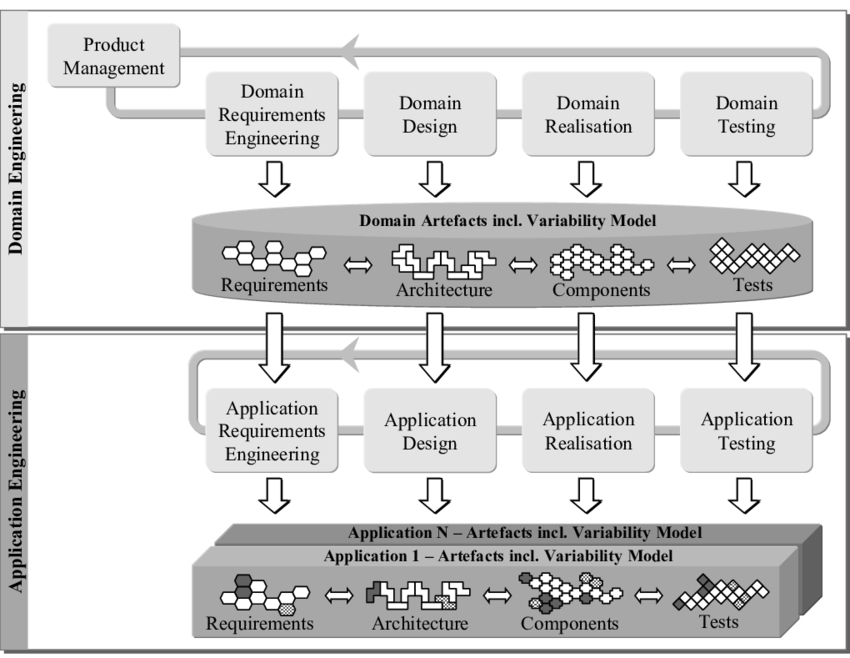
\includegraphics[width=110mm]{spldev-pohl}
	\caption{The \gls{SPL} development processes \cite{Pohl2005}}
	\label{fig:spldev}
\end{figure}

\gls{SPL} engineering consists in two development processes presented in Figure \ref{fig:spldev} \cite{Pohl2005}: \emph{domain engineering}, where \textit{commonalities and variabilities of the product line are defined and realised}, and \emph{application engineering}, where \textit{applications of the product line are built by reusing domain artefacts and exploiting the product line variability}. Each one of those two processes consists of several activities (including testing) and produces different artefacts. Domain artefacts are reused during application engineering in order to built one particular product. 

This thesis focuses on behavioural testing at the domain level. We seek to select \emph{relevant behaviours}, as well as \emph{relevant products} able to execute those behaviours in order to ensure that the \gls{SPL} fulfils its specification. To do so, we use a \emph{model-based} approach, with a model abstracting the behaviour of all the \gls{SPL} (including product-specific and SPL-common behaviours).

Commonalities and variabilities are captured trough the notion of \emph{feature}. A feature is a \textit{characteristic or end-user-visible behaviour of a software system} \cite{Apel2013}. It is a first-class abstraction that helps to reason about the \gls{SPL} \cite{Classen2008}. In practice, features are mapped to domain artefacts (or parts of domain artefacts) that are combined to form products. The derivation of one product consists in selecting a valid set of features, called \emph{configuration}, with the intended characteristics of the product, and combining the domain artefacts linked to those features. All the valid combinations of features are described in a \emph{feature model}.


%%%%%%%%%%%%%%%%%%%%%%%%%%%%%%%%%%%%%%%%%%%%%%%%%%
\section{Feature models}
%%%%%%%%%%%%%%%%%%%%%%%%%%%%%%%%%%%%%%%%%%%%%%%%%%

\label{sec:features}

\glsreset{FM}

\glspl{FM} describe all the valid combinations of features for \glspl{SPL}. They have been introduced by Kang \etal in the \gls{FODA} method \cite{Kang1990} using a graphical representation. Lot of other graphical \cite{Antkiewicz2004,Trinidad2008,Beuche2013,Leich2005} and textual \cite{Mendonca2009,Classen2011a} representations have been proposed and formalised \cite{Schobbens2007,Batory2005} since. In this thesis, we focus on graphical boolean \glspl{FM} and their equivalence in \gls{TVL} \cite{Classen2011a}. 

\begin{figure}
	\centering
	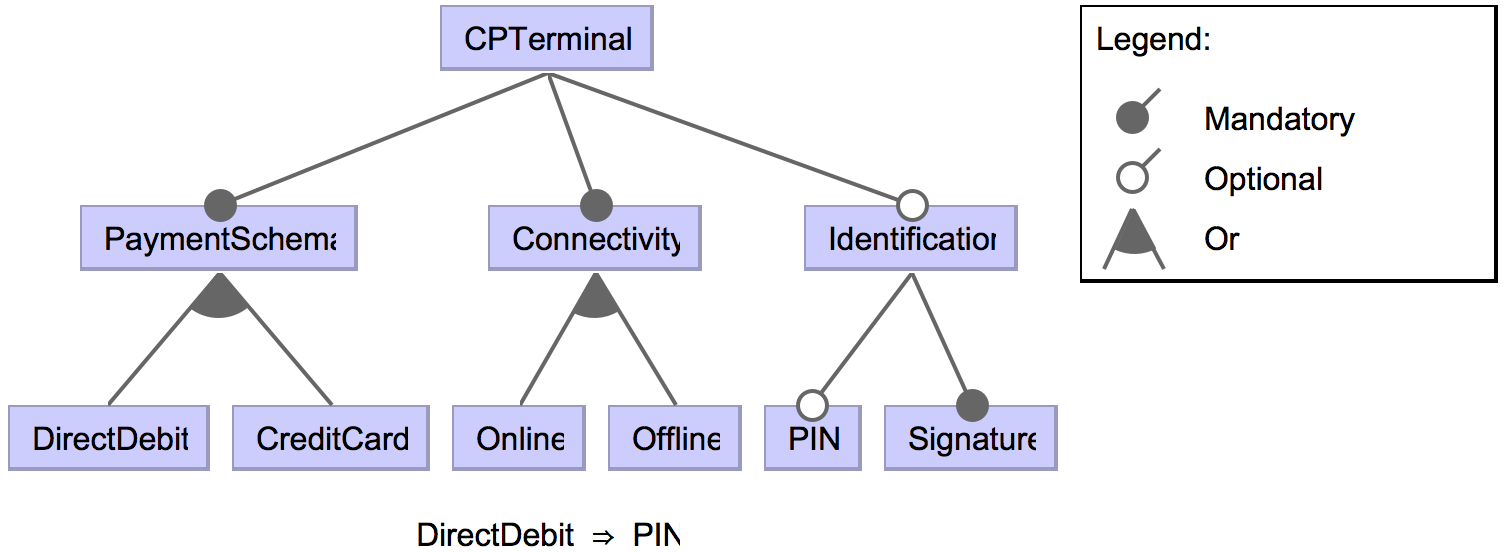
\includegraphics[width=100mm]{cpterminal-simplified-fm}
	\caption{Card payment terminal simplified feature model}
	\label{fig:cpterminalsimplifiedfm}
\end{figure}

A \gls{feature model} is organised in a tree-like structure (formally a directed acyclic graph). The root feature, always present in all products, is decomposed in sub-features using \textit{and} (all sub-features are selected if the parent feature is selected), \textit{or} (at-least one sub-feature is selected if the parent feature is selected), and \textit{xor} (exactly one sub-feature is selected if the parent feature is selected) relations. For instance, Figure \ref{fig:cpterminalsimplifiedfm} presents a (simplified) feature model for a card payment terminal product line. Root feature (\textit{CPTerminal}) is decomposed into two mandatory features (\textit{Pay\-ment\-Sche\-ma} and \textit{Con\-necti\-vi\-ty}) and one optional feature (\textit{Iden\-ti\-fica\-tion}). \textit{Pay\-ment\-Sche\-ma} (specifying if the terminal supports credit or debit cards) and \textit{Con\-necti\-vi\-ty} (specifying if the terminal is connected or not) features are decomposed into sub-features using a \textit{or} relation. Additionally, feature models may have cross-tree constraints expressed as boolean expressions over the features, \eg  \textit{Di\-rect\-De\-bit} $\Rightarrow$ \textit{PIN}, specifying that debit card payment requires PIN authentication.

\begin{lstlisting}[language=TVL,
float,
label=lst:cpterminalsimplifiedtvl,
caption={Card payment terminal simplified feature model in TVL format}]
root CPTerminal {
	group allOf {
		PaymentSchema,
		Connectivity,
		opt Identification
	}
} 

PaymentSchema {
	group someOf {
		DirectDebit,
		CreditCard
	}
	DirectDebit -> PIN; (*@\label{lst:cpterminalsimplifiedtvl:line:constraint}@*)
} 

Connectivity group someOf {
	Online,
	Offline
}

Identification group allof {
	opt PIN,
	Signature
}
\end{lstlisting}

Listing \ref{lst:cpterminalsimplifiedtvl} presents the TVL version of Figure \ref{fig:cpterminalsimplifiedfm}. In this case, features are decomposed in sub-features using \texttt{allOf} (\textit{and}), \texttt{someOf} (\textit{or}), or \texttt{oneOf} (\textit{xor}) relations. Additional cross-tree constraints (on line \ref{lst:cpterminalsimplifiedtvl:line:constraint}) may be specified and optional features are indicated using \texttt{opt} keyword.

The semantics of a feature model $d$, denoted $\Sem{d}$, corresponds to all the valid products allowed by the feature model. In the remainder of this thesis, we consider only \emph{boolean feature models}, \ie feature models where features have boolean values: \textit{true} if the feature is selected and \textit{false} otherwise. Since a boolean feature model may be transformed into a \gls{CNF} formula \cite{Batory2005}, denoted $\CNF(d)$, its semantics corresponds to all the feature assignments that satisfies this formula. This may be computed using \gls{SAT} or \gls{BDD} solvers \cite{Liang2015,Mendonca2008}.


%%%%%%%%%%%%%%%%%%%%%%%%%%%%%%%%%%%%%%%%%%%%%%%%%%%%%%%%%%%%%
\section{Behavioural modellisations of software product lines}
%%%%%%%%%%%%%%%%%%%%%%%%%%%%%%%%%%%%%%%%%%%%%%%%%%%%%%%%%%%%%

\label{sec:splbehaviouralmodeling}

Modern software systems are complex to build and maintain, counting thousands of lines of codes to achieve various purposes under different kinds of constraints (\eg time response, security, availability, \etc). To manage this complexity, software engineers use modeling \cite{swebok2014}. This allows to abstract the system by focusing on some of its aspects. For instance, feature models focus on the features of a product line and their constraints. In \gls{SPL} engineering, complexity worsen due to the variability inherent to product line. Models have to take features into account to represent this variability.

This section presents different modelling approaches to represent the behaviour of a software product line. Those approaches may be decomposed into two categories \cite{Apel2013}: \emph{annotation}-based approaches and \emph{composition}-based approaches. Annotation-based approaches annotate a common model to indicate which parts of the model belongs to which feature(s). During product derivation (\ie selection of the features of a product), parts of the model marked with unselected features are removed to give a model of the product. Composition-based approaches models features as a set of composable model parts. During product derivation, those parts are combined to form the model of the product. 

%----------------------------------------------------
\subsection{Composition-based modelling approaches}
%----------------------------------------------------

\begin{figure}[t]
	\centering
	\subbottom[Base model]{
		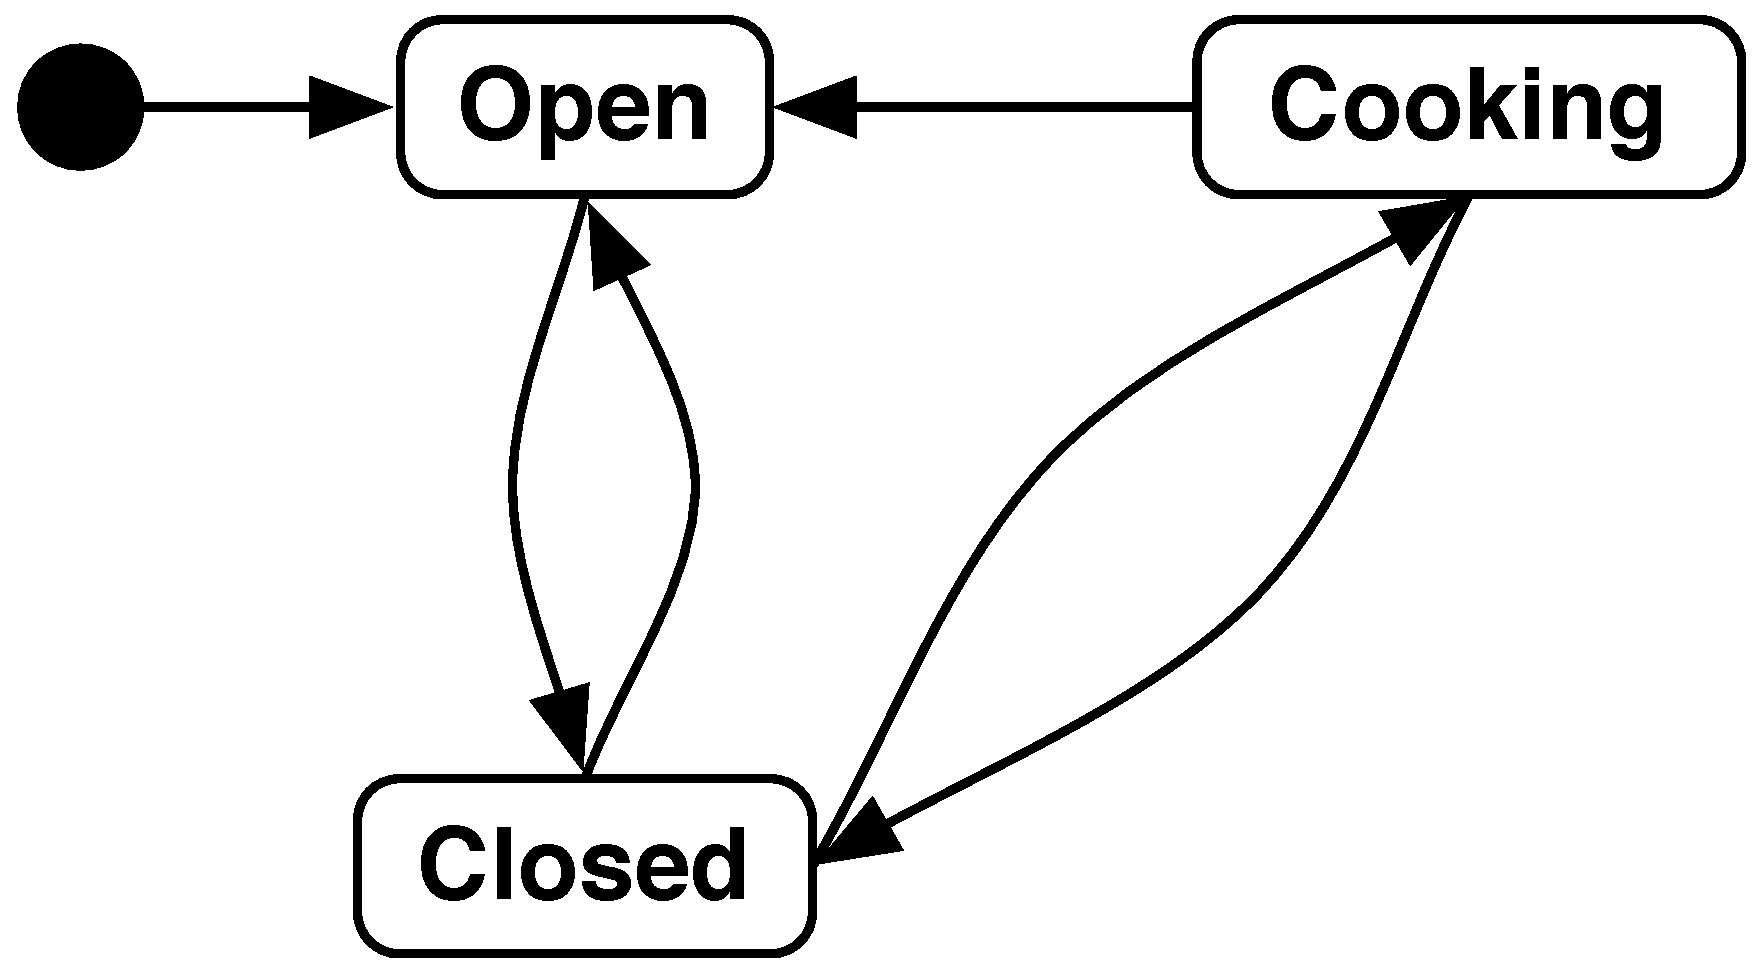
\includegraphics[width=38mm]{aom-base}
		\label{fig:aombase}
	}	
	\subbottom[Feature aspect]{
		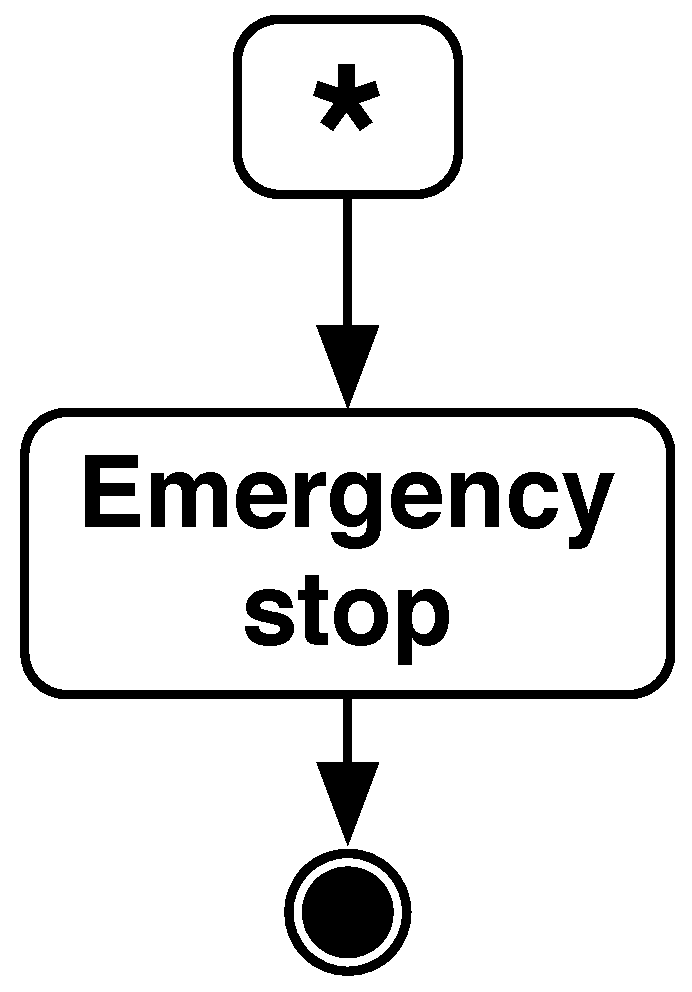
\includegraphics[width=14mm]{aom-aspect}
		\label{fig:aomaspect}
	}	
	\subbottom[Product model]{
		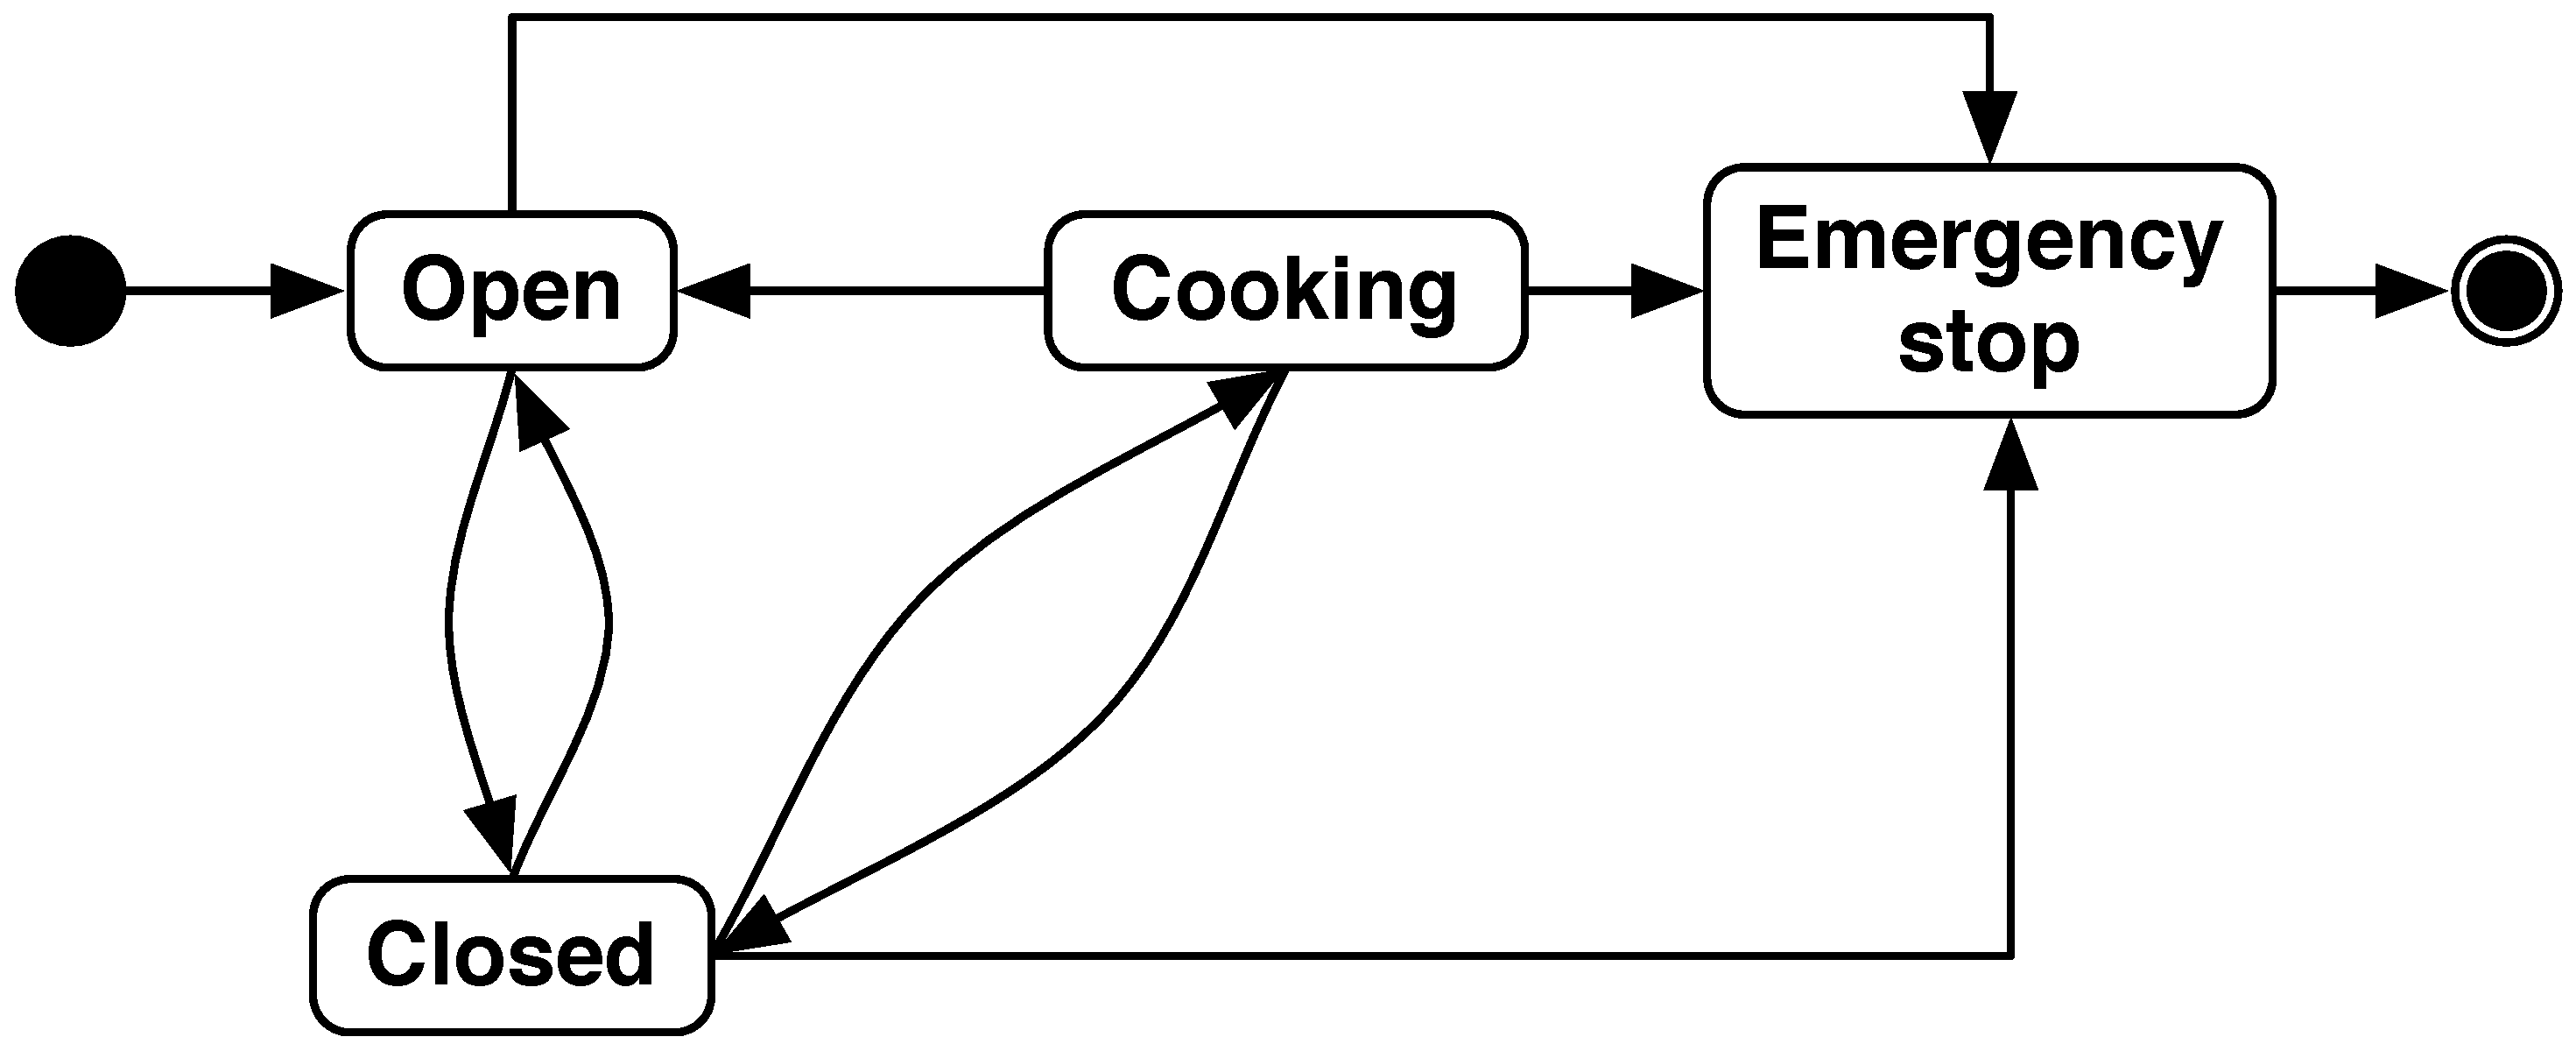
\includegraphics[width=54mm]{aom-result}
		\label{fig:aomresult}
	}
	\caption{\gls{SPL} behavioural composition-based modelling example \cite{Rashid2011}}
\end{figure}

Most composition-based modelling approaches are based on \emph{aspect oriented modelling} \cite{Rashid2011,Groher2009}. A base model representing the behaviour common to al the products of the product line is modified by weaving aspects specific to one or more features. For instance, Figure \ref{fig:aombase} presents the state machine base model of a oven in a smart home \cite{Rashid2011}. When a product with the feature \textit{emergency stop} is derived, the aspect from Figure \ref{fig:aomaspect} is weaved in the base model to give the state machine of the product in Figure \ref{fig:aomresult}. To decide where to be applied, the aspect must specify one or more pointcuts using a pointcut expression: '\texttt{*}' in Figure \ref{fig:aomaspect}.

Various formalisms based on transition systems \cite{Asirelli2012,Li2002,Li2002a,Li2005,Krishnamurthi2004,Fisler2001,Cordy2012} and Input-Output automata \cite{Lauenroth2009,Lauenroth2010} exist. Other composition-based modelling approaches are extensions of existing modelling languages where feature aspects may be weaved at some specific points of the system \cite{Altisen2006,Apel2010,Batory2008,Calder2006,Gondal2011,Schaefer2010,Millo2012a,Nelson2001,Poppleton2007,Sorge2009}. Finally, UML models like state machines \cite{Shaker2012,Shaker2012a} and sequence diagrams \cite{Greenyer2012} have been extended to support composition-based modelling.


%----------------------------------------------------
\subsection{Annotation-based modelling approaches}
%----------------------------------------------------

There exists several annotation-based modelling approaches to represent the behaviour of a software product line. Most of them consider a based model annotated with variability information indicating which products of the product line it belongs to. State-based models include for instance Petri nets \cite{Muschevici2010,Puschel2012,Heuer2013}, modal I/O automata \cite{Larsen2007}, \glspl{MTS} \cite{Asirelli2011,Asirelli2011a,Asirelli2011b,Fantechi2008,Fischbein2006,TerBeek2013,terBeek2011}, \glspl{FTS} \cite{Classen2011-thesis,Classen2013b,Classen2011,Classen2010}, and finite state machines \cite{Sabouri2012,Sabouri2012}. Other formalisms include PL-CSS  (a process algebra) \cite{Gruler2008} and higher-level formalisms like UML activity diagrams \cite{Heuer2013}. 

\glsreset{LTS}

Researches on annotation-based models for software product line verification have been conducted for years and are still developed by the model-checking community. Amongst all the existing notations, in this thesis, we focus on those derived from \gls{LTS}, a simple and yet expressive formalism to model the behaviour of a system:
%
\begin{definition}[\acrfull{LTS} \cite{Baier2008}] \label{def:ts}
A LTS is a tuple $(S,$ $\Act,$ $\trans,$ $i)$, where:
\begin{itemize}
\item $S$ is a set of \emph{states};
\item $\Act$ is a set of \emph{actions};
\item $\trans \ \subseteq S \times \Act \times S$ is a \emph{transition} relation (with $(s_1, \alpha, s_2) \in \trans$, denoted $s_1 \overset{\alpha}{\longrightarrow} s_2$);
\item and $i \in S$ is the \emph{initial state}.
\end{itemize}
\end{definition} 
%
This choice is motivated by the existence of powerful modelling languages \cite{Asirelli2011a,Fantechi2008,TerBeek2013}, algorithms \cite{Classen2010,Classen2013b}, and tools \cite{Asirelli2011b,Cordy2013} developed by the model-checking community. Also, lot of other higher-level formalisms may be translated to \gls{LTS} \cite{Devroey2015c} allowing to make our results easily applicable to other modelling  languages.

%-------------------------------------------
\subsection{Featured transition system}
%-------------------------------------------

\begin{figure}[t]
	\centering
	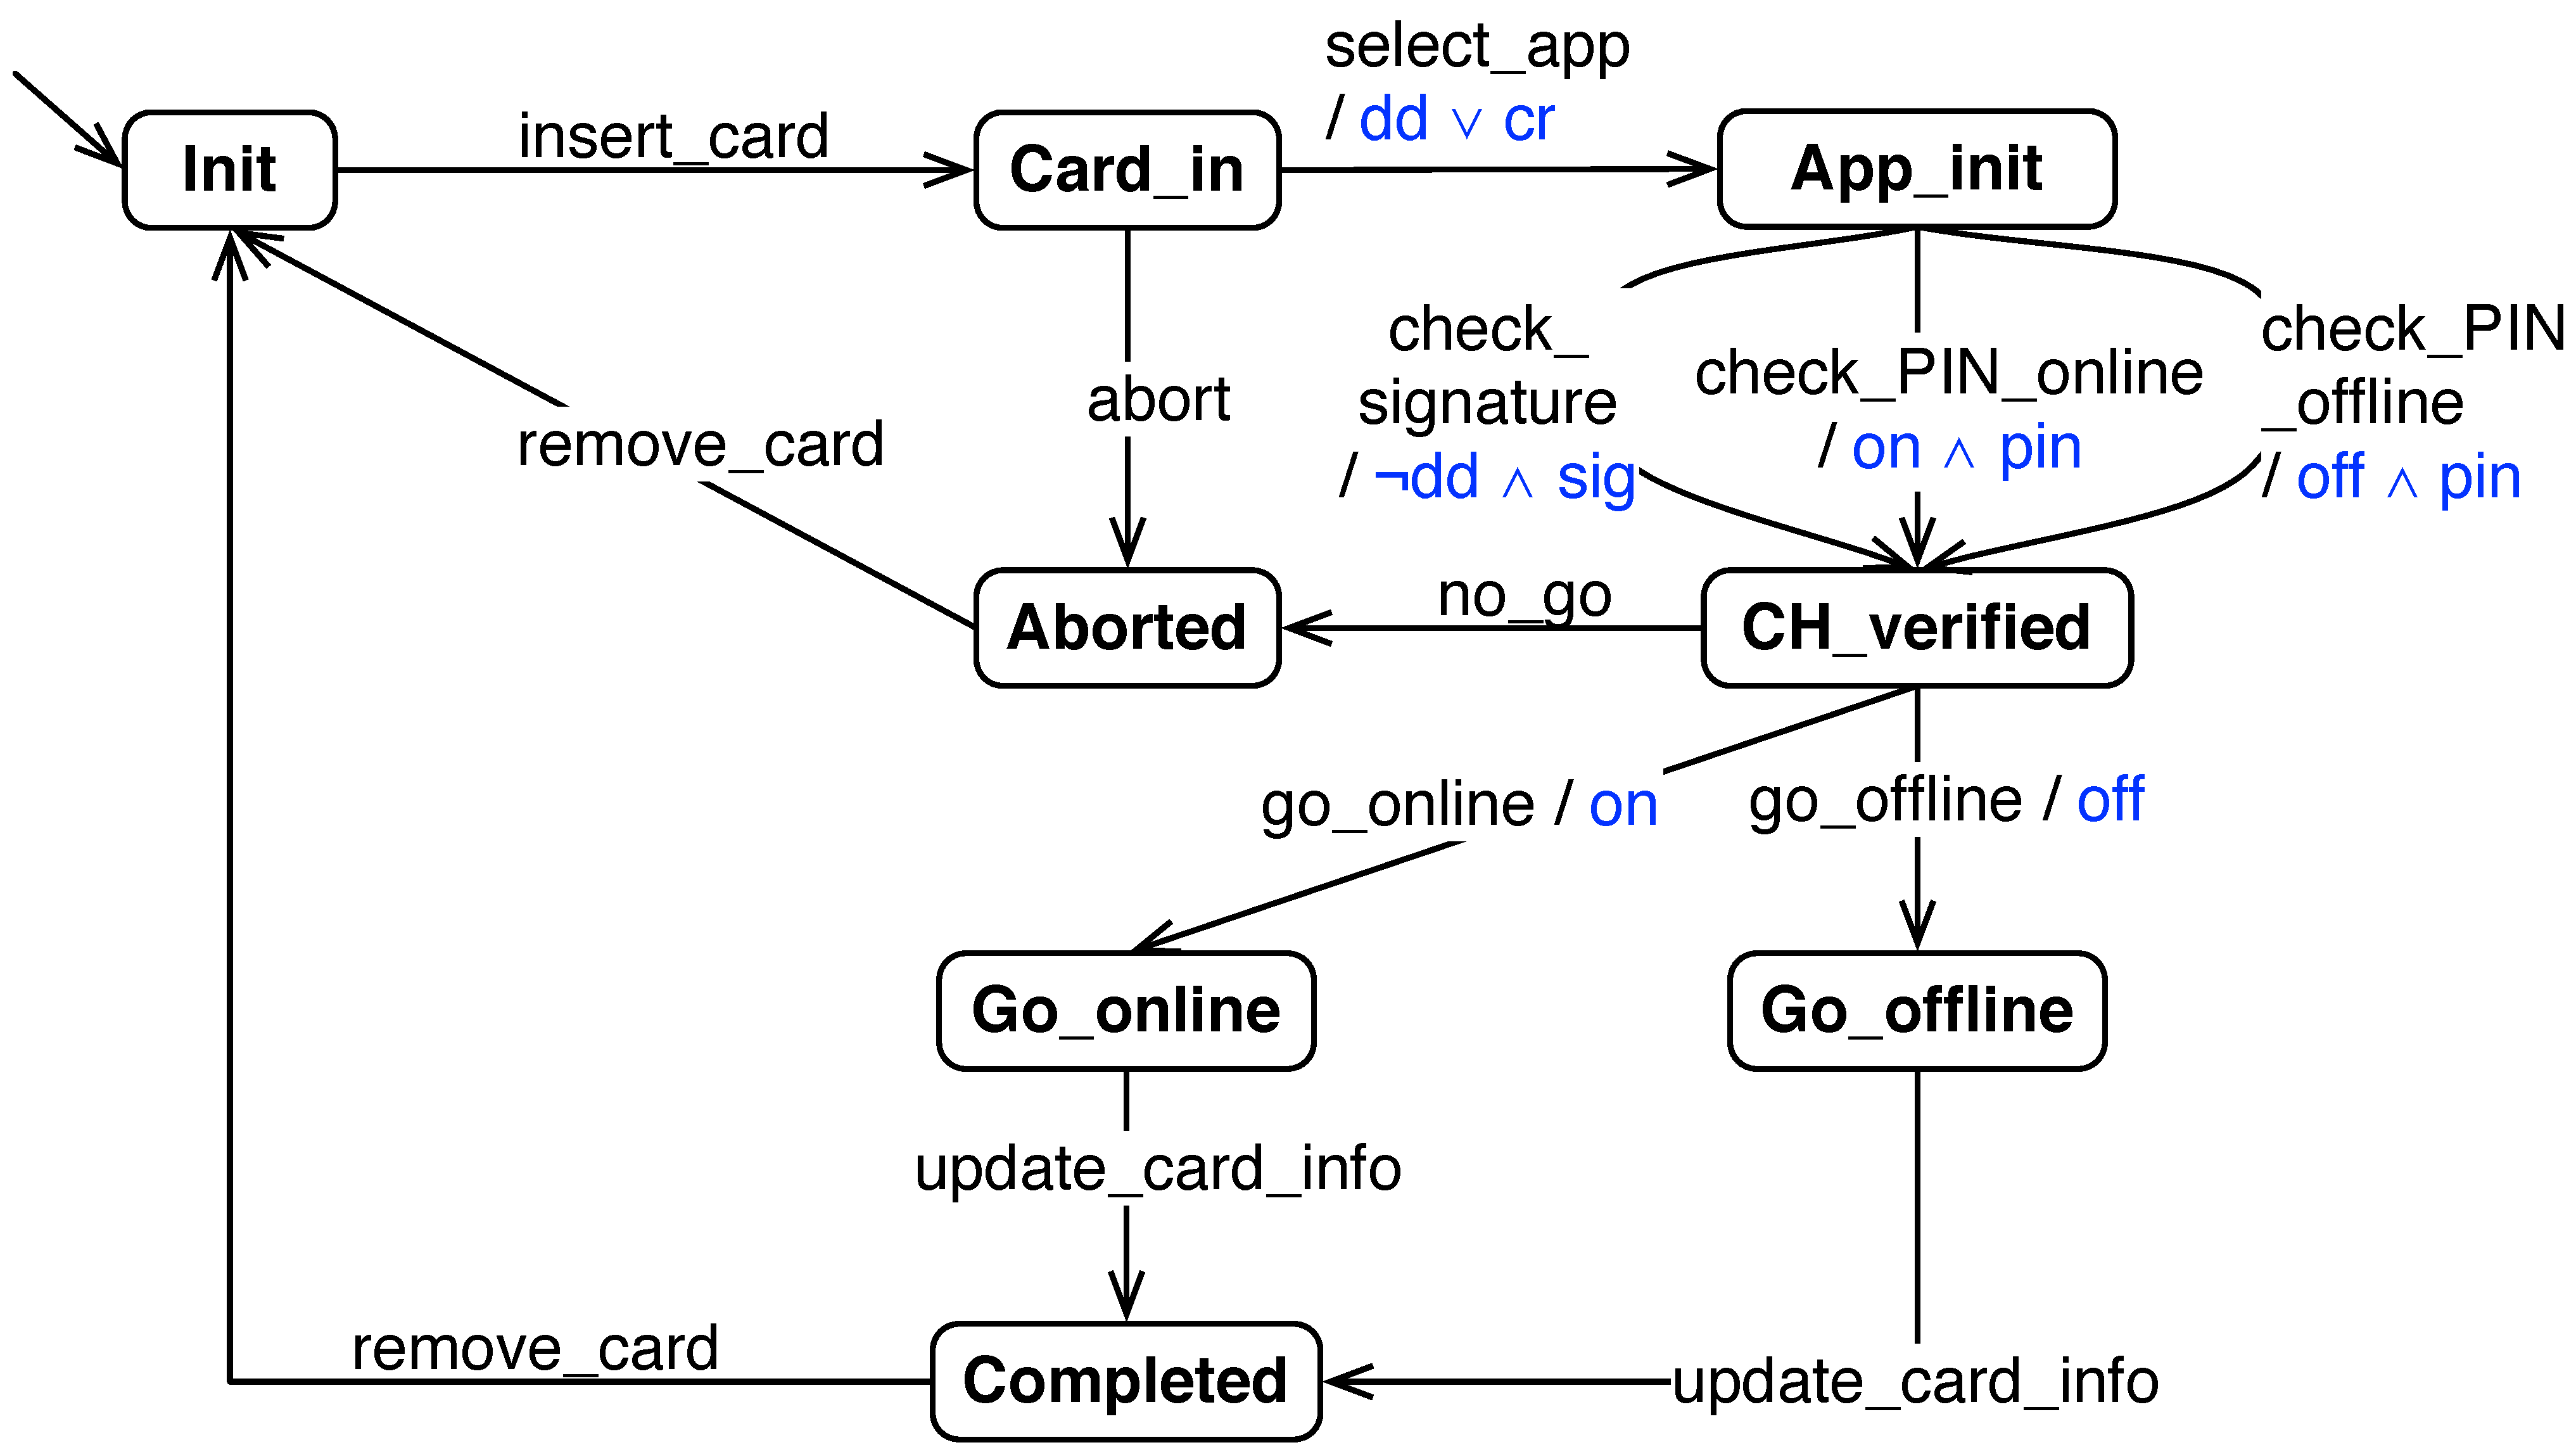
\includegraphics[width=100mm]{cpterminal-simplified-fts}
	\caption{Card payment terminal simplified \gls{featured transition system}}
	\label{fig:cpterminalsimplifiedfts}
\end{figure}

\glsreset{FTS}

Classen \etal \cite{Classen2013b} define \gls{FTS} to represent the behaviour of a product line. An \gls{FTS} is an \gls{LTS} where transitions have been annotated with feature expressions defining which products of the \gls{feature model} is able to execute the transition. For instance, the \gls{FTS} in Figure \ref{fig:cpterminalsimplifiedfts} presents the behaviour of all the products of the card payment terminal product line. The feature expressions on the transitions references the features of the feature model in Figure \ref{fig:cpterminalsimplifiedfm}. First, the terminal is initialised (\textit{Init}) and ready to proceed card payments. When a card is inserted, the terminal selects an appropriate payment method and launches the corresponding application (\textit{App\_init}). This can only be done if the terminal processes debit or credit cards, denoted by the feature expression $\mathit{dd} \vee \mathit{cr}$. Next step is to identify the card holder, either by using a \gls{PIN} code, which can be done online ($on \wedge pin$) of offline ($\mathit{off} \wedge \mathit{pin}$), or a signature if the terminal does not process debit cards ($\neg \mathit{dd} \wedge \mathit{sig}$). If the identification succeeds (\textit{CH\_Verified}), the terminal process the transaction online (\textit{Go\_online}) or offline (\textit{Go\_offline}), updates the information on the card, and completes the transaction (\textit{Completed}). Formally, \glspl{FTS} are defined as follows:
%
\begin{definition}[\acrfull{FTS} \cite{Classen2013b}]
\label{def:fts}
A \gls{FTS} is a tuple $(S,$ $\Act,$ $\trans,$ $i,$ $d,$ $\gamma)$, where:
\begin{itemize}
\item $S$, $\Act$, $\trans$, $i$ are defined according to definition \ref{def:ts}; 
\item $d$ is a \emph{feature model}; 
\item $\gamma: \trans \mapsto \Sem{d} \mapsto \mathbb{B}$  is a labelling function specifying for each transition which valid products may execute it; this function is represented as a boolean expression over the features of $d$, called \emph{\gls{feature expression}}.
\end{itemize}
\end{definition}

\begin{figure}[t]
	\centering
	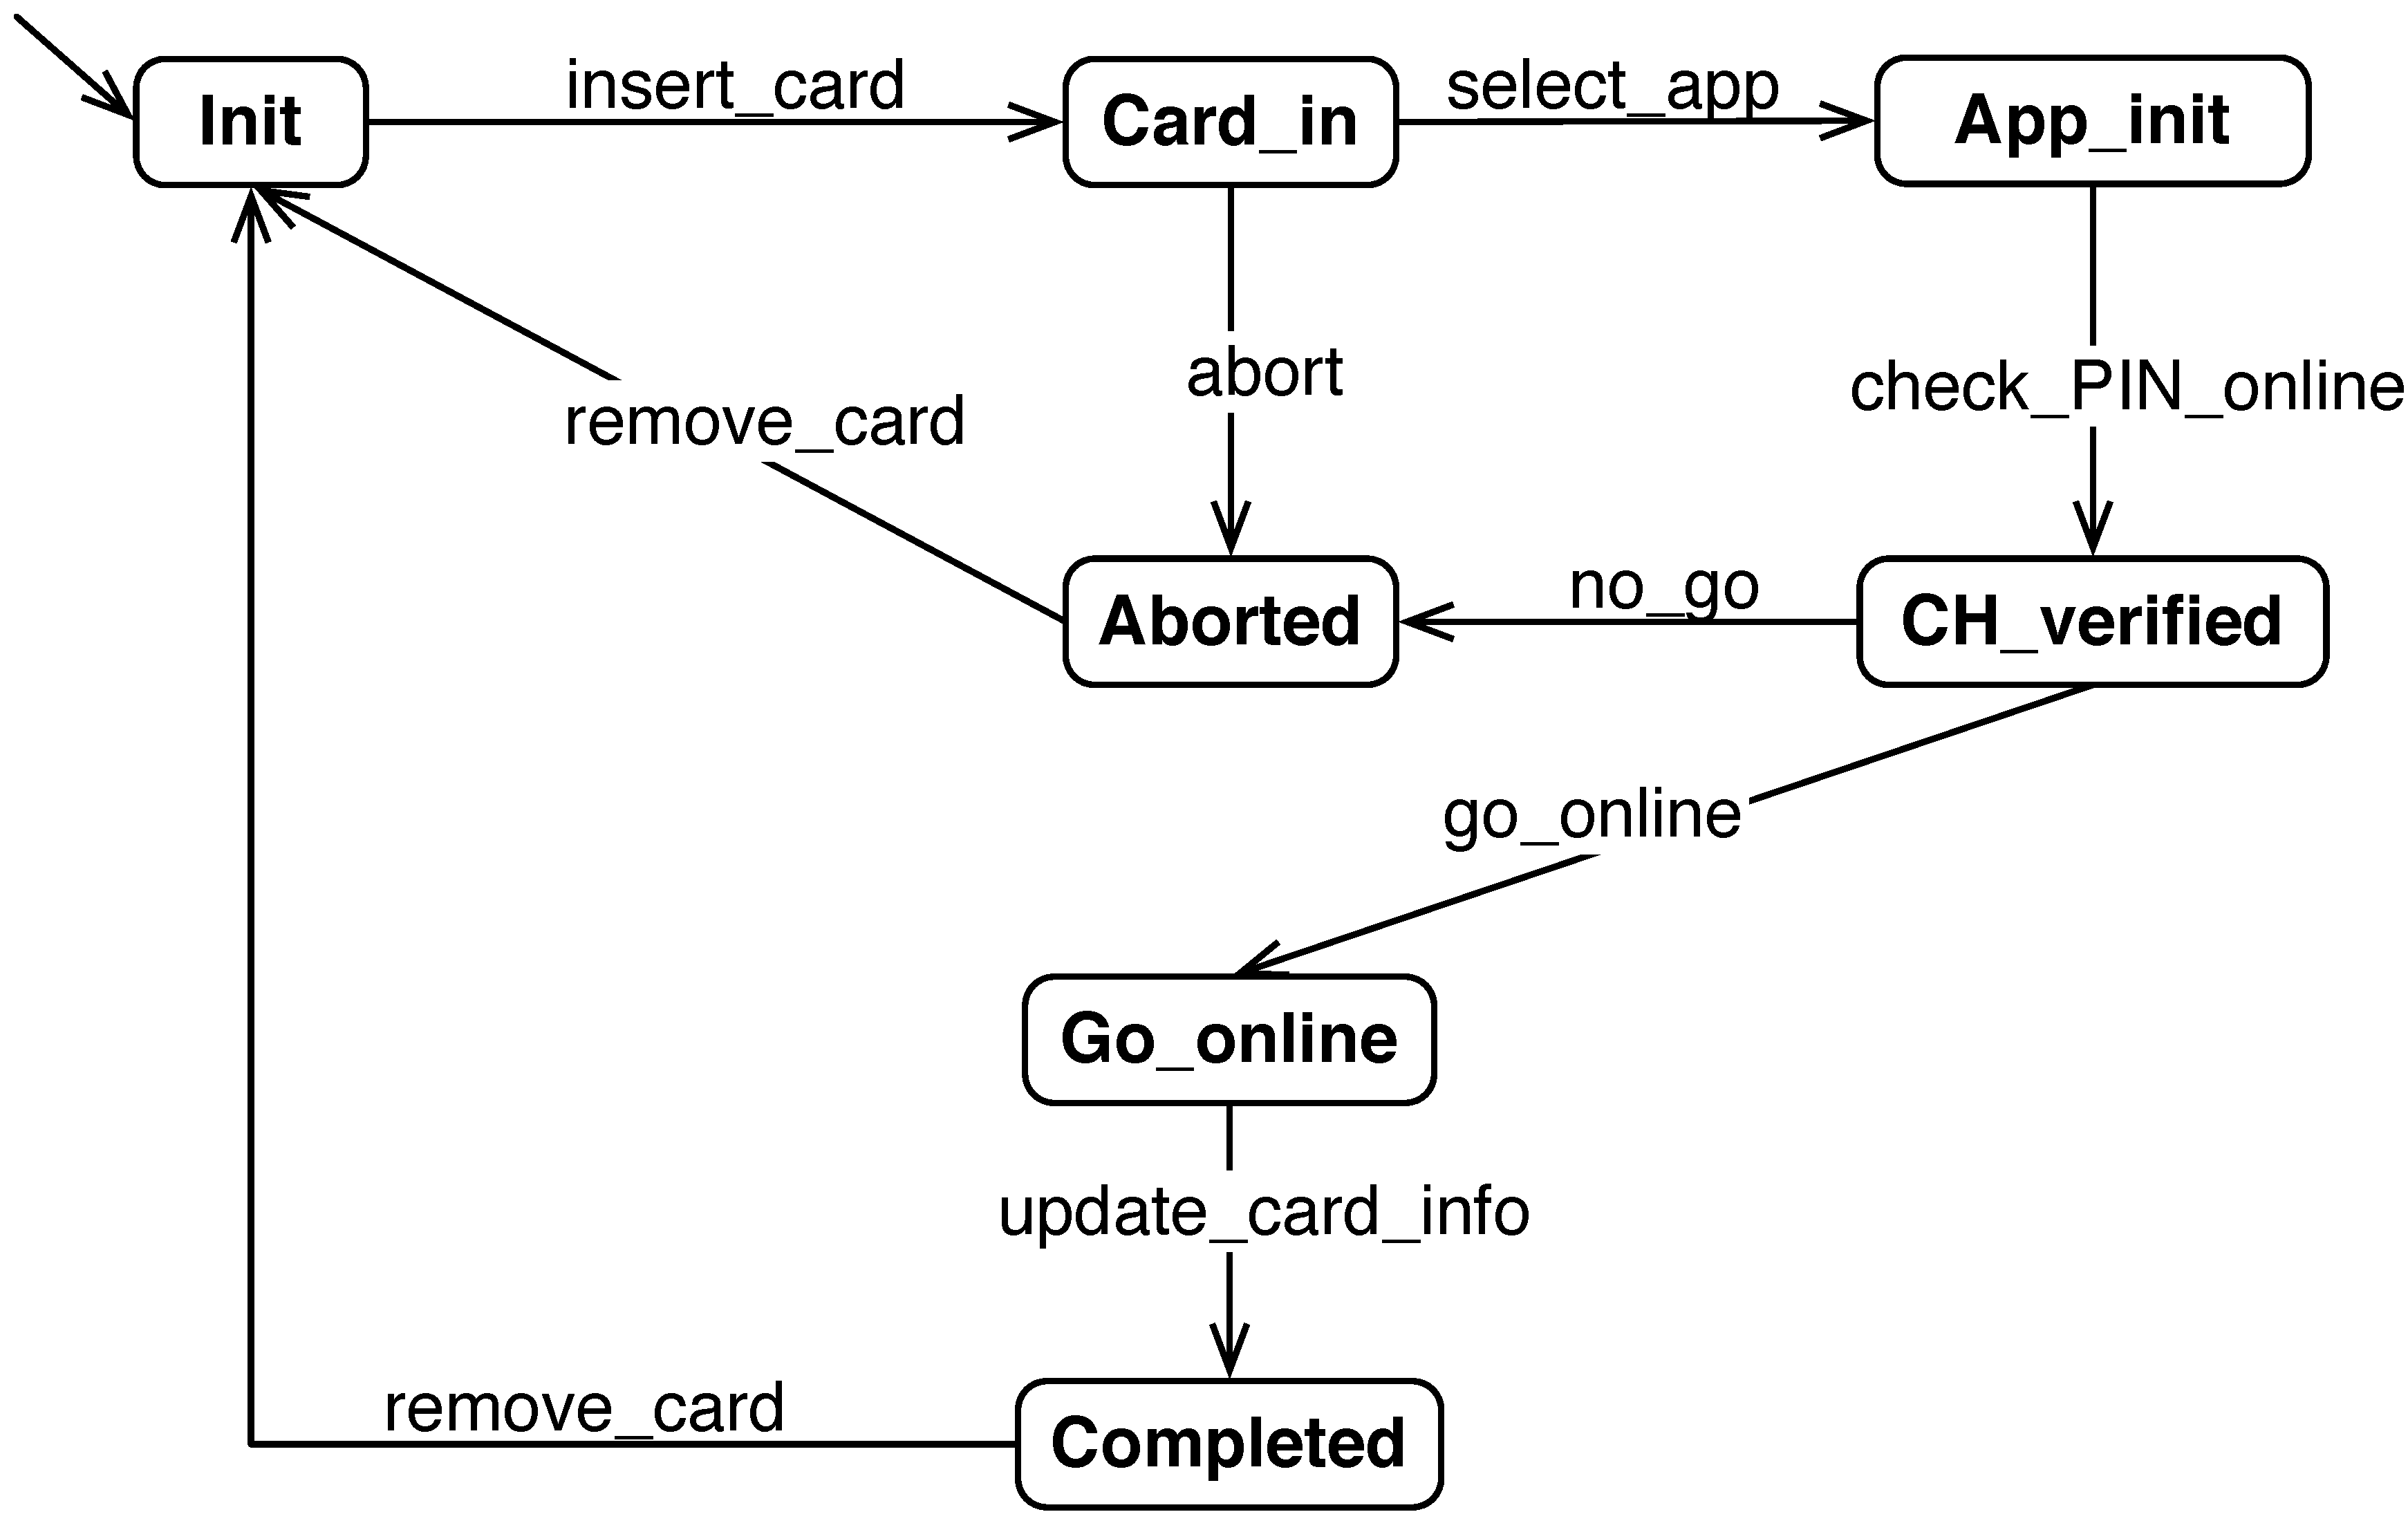
\includegraphics[width=90mm]{cpterminal-projection}
	\caption{Card payment terminal product \gls{LTS}}
	\label{fig:cpterminalprojection}
\end{figure}


\paragraph{FTS projection:}
%------------------------------

To derive the \gls{LTS} of one particular card payment terminal product, the \gls{FTS} is \emph{projected} \cite{Classen2010,Classen2013b} on this product by pruning the transitions whose feature expressions are not satisfied and by removing the feature expressions. For instance, Figure \ref{fig:cpterminalprojection} is the projection of the \gls{FTS} in Figure \ref{fig:cpterminalsimplifiedfts} on the card payment terminal product supporting direct debit (\textit{dd}) cards, with a \gls{PIN} identification (\textit{pin}) and an online connection (\textit{online}). Formally, the projection operator is defined as follows:
%
\begin{definition}[Projection operator \cite{Classen2013b}]
Let $\fts = (S,$ $\Act,$ $\trans,$ $i,$ $d,$ $\gamma)$ be an \gls{FTS}, and $p\in \Sem{d}$ be a product of the feature model $d$. The projection of $\fts$ onto $p$, denoted $\fts_{\mid p}$, is the \gls{LTS} $(S,$ $\Act,$ $\trans',$ $i)$ where
$$ \trans' = \left\lbrace \mathit{tr} \in \trans \mid \wSAT\left(p \wedge \gamma(\mathit{tr})\right) \right\rbrace $$
Where \gls{SAT} checks the satisfiability of the feature expression labelling the transition giving the product $p$.
\end{definition}


\paragraph{Deterministic FTS:}
%-----------------------------

As for \glspl{LTS}, an \gls{FTS} is deterministic if, for all sequence of actions, there is at most one possible path (sequence of transitions) for those actions. Since \gls{FTS} models the behaviour of all the products of a product line, it moreover requires to have satisfiable feature expressions on this path.
%
\begin{property}[Deterministic FTS]
An \gls{FTS} $(S,$ $\Act,$ $\trans,$ $i,$ $d,$ $\gamma)$ is deterministic if:
\begin{multline*}
\forall (\alpha_1, \ldots, \alpha_n) \in \left(\Act \cup \left\lbrace \epsilon \right\rbrace\right) ^{*},
\exists \text{ at most one } \mathit{seq} = i \xrightarrow{\alpha_1} \ldots \xrightarrow{\alpha_m} s_k \\
\text{ such that } \wSAT\left( \CNF(d) \wedge \bigwedge_{\mathit{tr} \in \mathit{seq}} \gamma(\mathit{tr}) \right)
\end{multline*}
\end{property}
%
Checking if an \gls{FTS} is deterministic is computationally heavy. In the worst case, it requires a complete exploration of the model with multiple \gls{SAT} calls.


\paragraph{Connected FTS:}
%-----------------------------

A connected \gls{FTS} is an \gls{FTS} that has no isolated state. All states may be reached from the initial state and reach back the initial state, \ie for each state, there exists a path starting from the initial state and going back to the initial state.
%
\begin{property}[Connected FTS]
An \gls{FTS} $(S,$ $\Act,$ $\trans,$ $i,$ $d,$ $\gamma)$ is connected if:
$$
\forall s \in S, \exists \mathit{seq} = i \xrightarrow{\alpha_1} \ldots \xrightarrow{\alpha_m} s \xrightarrow{\alpha_n} \ldots \xrightarrow{\alpha_o} i \text{ such that } \wSAT\left( \CNF(d) \wedge \bigwedge_{\mathit{tr} \in \mathit{seq}} \gamma(\mathit{tr}) \right)
$$
\end{property}
%
One may use (for instance) an accessibility matrix (see Algorithm \ref{algo:warshall} from Section \ref{subsec:allstatesselection}) to check that there is no isolated state. In the remainder of this thesis, most of our algorithms assume connected \glspl{FTS}.

%-------------------------------------------
\subsection{Related work}
%-------------------------------------------

We choose \gls{FTS} as formalism to model the behaviour of \glspl{SPL} over \gls{MTS} \cite{Fischbein2006} and PL-CSS \cite{Gruler2008}. \gls{MTS} is an extension of \gls{LTS} where the set of transitions is partitioned into \textit{may} and \textit{must} transitions. \textit{Must} transitions are transitions fired by all the products of the product line, while \textit{may} transitions are fired by only some (undetermined) products of the product line. To relate a transition to the exact set of products able to execute it, Asirelli \etal \cite{Asirelli2012,Asirelli2011b,Asirelli2011a} associates \gls{MTS} to a branching-time temporal logic named \gls{MHML} representing the constraints between the features and the actions. The \gls{MHML} formula may be derived from a feature model (representing those constraints) and the associated \gls{MTS} but makes the relation between products and transitions unclear.

\gls{PL-CCS} \cite{Gruler2008} is a process calculus extending Milners's \gls{CCS} \cite{Milner1982} by adding a \textit{binary variant} operator to represent alternatives features in a \gls{SPL}. As for \glspl{MTS}, PL-CSS does not include constraints between features and relies on an external \textit{mu}-calculus \cite{Shoham2012} to express them.

In their work, Beohar \etal \cite{Beohar2015} analyse the \emph{expressiveness} of \gls{FTS}, \gls{MTS}, and PL-CCS by comparing the set of products they can specify. Products specifications are represented using \glspl{LTS}. They demonstrate that \gls{FTS} is the most expressive formalism, followed by \gls{PL-CCS} and \gls{MTS}. Meaning that \gls{MTS} models may be expressed using \gls{PL-CCS}, and \gls{PL-CCS} models may be expressed using \gls{FTS} but not (always) the other way around.


%%%%%%%%%%%%%%%%%%%%%%
\section{Wrap up}
%%%%%%%%%%%%%%%%%%%%%%

In this chapter, we presented the standard software product line engineering process and focuses on domain level to perform behavioural model-based testing, \ie selecting relevant products and behaviour to test in the product line. \gls{SPL} variability is encoded using a boolean \gls{feature model} and behaviour is described using an annotation-based formalism: a connected \gls{FTS}. We choose \glspl{FTS} for their expressiveness and the simplicity of their encoding allowing powerful algorithms \cite{Classen2013b,Cordy2013} while preserving a readable relation between transitions and products able to execute them.



%\chapter{Behavioural model based testing}
%\label{chap:mbt}
%
%%%%%%%%%%%%%%%%%%%%%%%%%%%%%%
\section{Software testing}
%%%%%%%%%%%%%%%%%%%%%%%%%%%%%%

Software testing is a process present in a majority of software system developments. According to Mathur's definitions \cite{Mathur2008}, it aims at evaluating if a software behaves as expected. When running a software system, one may face a \emph{\gls{failure}}, \ie an unexpected behaviour of the system. This failure is the propagation to the output of the system of one or more \emph{\glspl{bug}} (also called \emph{\glspl{fault}}), coming from \emph{\glspl{error}} made during the writing of the source code of the software system. The goal of a software testing process is to find as many bugs as possible in a given software system, called \acrfull{SUT}, in order to prevent failures to happen during the operation of the software system.

Another definition from the Software Engineering Body of Knowledge~\cite{swebok2014} defines software testing as follows:
%
\begin{quote}
Software testing consists of the \emph{dynamic} verification that a program provides \emph{expected} behaviours on a \emph{finite} set of test cases, suitably \emph{selected} from the usually infinite execution domain.
\end{quote}
%
This definition, although not specific on how to perform software testing, includes different important aspects. First, the SUT has to be \emph{executed} on a set of input values\footnote{In this case, input values may refer to input data or, more generally, to a specific input state of the SUT.} in order to observe its behaviour. Second, to decide if the SUT behaves as expected, it must be possible, based on the outcomes of the SUT for a given input, to decide if the outcomes are acceptable or not. This is also referred to as \emph{the oracle problem} \cite{swebok2014}. Finally, the number of observed behaviour exercised by the test cases is \emph{finite}: a software testing process is the result of a trade-off between limited resources, schedules, and unlimited rest requirements. Therefore, the \emph{\gls{test suite}} (\ie the set of test cases) has to be properly selected in order to satisfy this trade-off using \emph{\gls{selection criteria}}.

The software testing process itself may be implemented in various ways. Tretmans~\cite{Tretmans2004,Utting2007} defines a typology of software testing processes based on three dimensions: the characteristic being tested, the scale of the SUT, and the information used to select test cases.

\paragraph{Characteristic being tested:} 
%
The most common characteristic being tested is the functionality (\emph{functional testing}), which aims at checking that a SUT produces a correct output for a given input. Other characteristics includes (but are not limited to) robustness (\emph{robustness testing}), which aims at checking that the SUT can resist to invalid conditions in its environment (\eg wrong inputs, hardware failures, network failures, other systems failures, \etc); performance (\emph{performance testing}), which aims at checking that the SUT can resist heavy loads; usability (\emph{usability testing}), which focuses on user interfaces problems; security (\emph{security testing}), which aims at checking that the system is not vulnerable to malicious users; \etc
 
\paragraph{Scale of the SUT:} 
%
It indicates which parts of the system are considered during the execution of each test case: \emph{unit testing} focuses on single units at a time (\eg a single method, a single function, a single class, \etc); \emph{component testing} tests each part of the system separately, while \emph{integration testing} checks that the different components work together correctly; finally, \emph{system testing} considers the whole system to perform testing.

\paragraph{Information used to select test cases:} 
%
Information may be either \emph{white box} or \emph{black box}. White box testing processes use the source code as input. They allow one to define selection criteria on the source code of the application: \eg statement coverage requires that each statement is executed at least once by one test case of the test suite. Black box testing processes will use the requirements of the SUT as input. In this case, the source code is not accessible and selection criteria are specified over the requirements: \eg input domain coverage requires to split the input domain in equivalence classes and to design test cases that will use at least one element of each class.


%%%%%%%%%%%%%%%%%%%%%%%%%%%%%%
\section{Model-based testing}
%%%%%%%%%%%%%%%%%%%%%%%%%%%%%%






\chapter{Software and software product lines testing}
\label{chap:vis-testing}
Software testing is a process present in a majority of software developments. According to Mathur's definitions \cite{Mathur2008}, it aims at evaluating if a software behaves as expected. When running a software system, one may face a \emph{\gls{failure}}, \ie an unexpected behaviour of the system. This failure is the propagation to the output of the system of one or more \emph{\glspl{bug}} (also called \emph{\glspl{fault}}), coming from \emph{\glspl{error}} made during the writing of the source code of the software system or resulting from earlier issues in specifications. The goal of a software testing process is to find as many bugs as possible in a given software system, called \acrfull{SUT}, in order to prevent failures to happen during the operation of the software system.

When it comes to product lines, testing becomes more complex. As the system under test is the set of products of this product line, using a standard testing process would require to derive all those products and, for each one of them, design and execute a test suite. This approach, called \emph{product-based} \cite{Thum2014}, is intractable for the large majority of product lines. \gls{SPL} testing requires to adapt standard testing process to minimize the effort by reusing testing assets from one product to another and prioritizing the products to test. To achieve this, most techniques adopt a model-based approach: \eg sampling a set of products to test from a feature model.

This chapter presents the state-of-the-art of SPL testing. Sections \ref{sec:softwaretesting} and \ref{sec:mbt} presents software testing and model-based testing, Section \ref{sec:spltesting} gives a view of \gls{SPL} testing, and Section \ref{sec:mbtspltesting} focuses on existing model-based approach to \gls{SPL} testing.


%%%%%%%%%%%%%%%%%%%%%%%%%%%%%%
\section{Software testing}
%%%%%%%%%%%%%%%%%%%%%%%%%%%%%%

\label{sec:softwaretesting}

The Software Engineering Body of Knowledge from the IEEE Computer Society \cite{swebok2014} defines software testing as follows:
%
\begin{quote}
Software testing consists of the \emph{dynamic} verification that a program provides \emph{expected} behaviours on a \emph{finite} set of test cases, suitably \emph{selected} from the usually infinite execution domain.
\end{quote}
%
This definition, although not specific on how to perform software testing, includes different important aspects. First, the SUT has to be \emph{executed} on a set of input values\footnote{In this case, input values may refer to input data or, more generally, to a specific input state of the SUT.} in order to observe its behaviour. Second, to decide if the SUT behaves as expected, it must be possible, based on the outcomes of the SUT for a given input, to decide if the outcomes are acceptable or not. This is also referred to as \emph{the oracle problem} \cite{swebok2014}. 
Finally, the number of observed behaviours exercised by the test cases is \emph{finite}: a software testing process is the result of a trade-off between limited resources, schedules, and unlimited test requirements. Therefore, the \emph{\gls{test suite}} (\ie the set of test cases) has to be properly selected in order to satisfy this trade-off using a \emph{criterion}.

The software testing process itself may be implemented in various ways. Tretmans~\cite{Tretmans2004,Utting2007} defines a typology of software testing processes based on three dimensions: the characteristic being tested, the scale of the SUT, and the information used to select test cases.

\paragraph{Characteristic being tested:} 
%
The main characteristic being tested is the functionality (\emph{functional testing}), which aims at checking that a SUT produces a correct output for a given input. Other characteristics includes (but are not limited to) robustness (\emph{robustness testing}), which aims at checking that the SUT can resist to invalid conditions in its environment (\eg wrong inputs, hardware failures, network failures, other systems failures, \etc); performance (\emph{performance testing}), which aims at checking that the SUT can resist heavy loads; usability (\emph{usability testing}), which focuses on user interfaces problems; security (\emph{security testing}), which aims at checking that the system is not vulnerable to malicious users; \etc In this thesis, we focus on functional testing.
 
\paragraph{Scale of the SUT:} 
%
It indicates which parts of the system are considered during the execution of each test case: \emph{unit testing} focuses on single units at a time (\eg a single method, a single function, a single class, \etc); \emph{component testing} tests each part of the system separately, while \emph{integration testing} checks that the different components work together correctly; finally, \emph{system testing} considers the whole system to perform testing.

\paragraph{Information used to select test cases:} 
%
Information may be either \emph{white box} or \emph{black box}. White box testing processes use the source code as input. They allow one to define selection criteria on the source code of the application: \eg statement coverage requires that each statement is executed at least once by one test case of the test suite. Black box testing processes will use the requirements of the SUT as input. In this case, the source code is not accessible and selection criteria are specified over the requirements: \eg input domain coverage requires to split the input domain in equivalence classes and to design test cases that will use at least one element of each class.

Most of the time, the selection of a test suite is done manually. For instance, it is very common for developers to write functional unit tests for their code before submitting it to a version control system. In most cases and with the right tool support, this may be enough. However, manual testing becomes expensive for larger systems, especially during integration and system testing \cite{Utting2007}. 

%%%%%%%%%%%%%%%%%%%%%%%%%%%%%%
\section{Model-based testing}
%%%%%%%%%%%%%%%%%%%%%%%%%%%%%%

\label{sec:mbt}

\begin{figure}
	\centering
	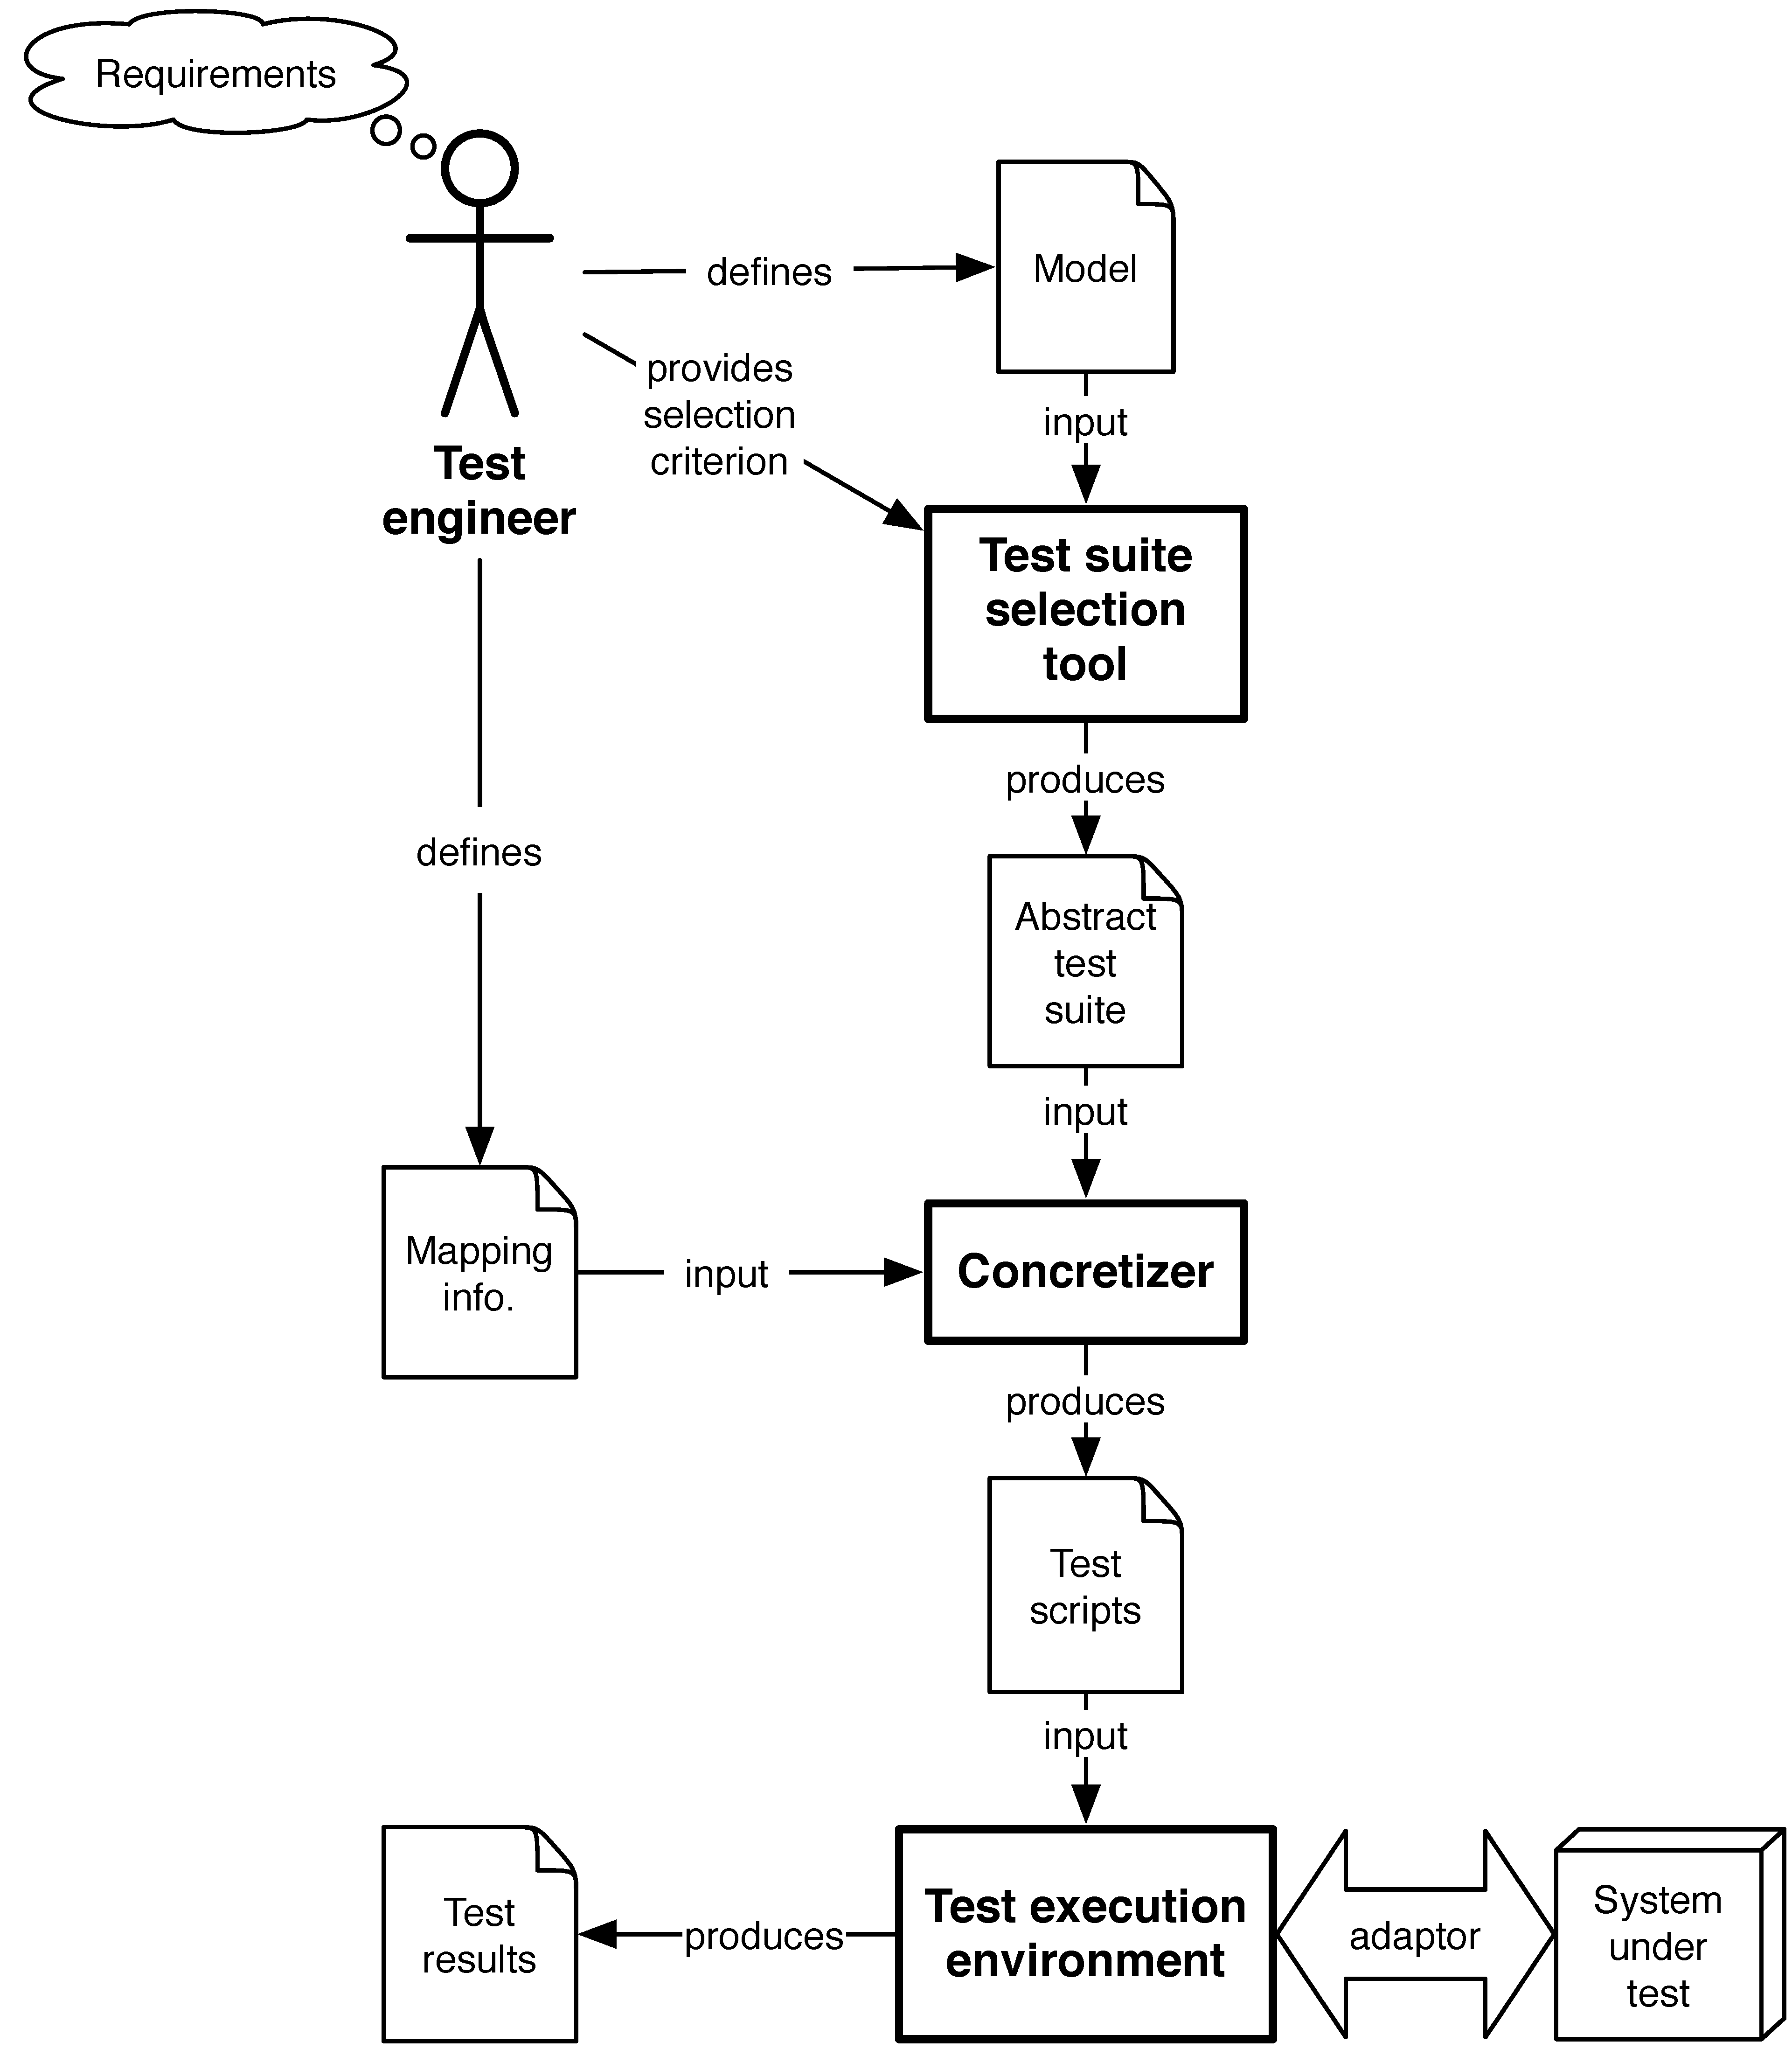
\includegraphics[width=110mm]{mbt-process}
	\caption{Model-based testing process}
	\label{fig:mbtprocess}
\end{figure}

Automating test suite selection is not easy though. It requires an \emph{input generator} that, for each test case, generates a sequence of input operations for the system (\eg a sequence of method calls); an \emph{oracle} which decides, based on the input sequence and the outputs of the system if the test case is pass or fail; and a \emph{selection criterion} (with a mechanism to measure it) in order to decide when to stop the selection. For instance, EvoSuite \cite{Fraser2011} is a white box Java test cases generator that uses an evolutionary algorithm to generate JUnits by analysing methods paths. Since the tool only uses the source code as input, the oracle is very limited and can only tell if a test case execution should throw an exception or not. To improve this oracle, it requires to analyse the specification of the methods to foretell the expected output.

An alternative is to use a semi-automated approach: \emph{model-based testing} \cite{Utting2007}. It requires to define a model of the expected behaviour of the SUT (\ie a specification) that serves as input to an automated test suite selection tool. The model should be small enough to be cheaper than the analysis of the actual system, but accurate enough to describe the characteristics to test. The tool uses this model to generate a sequence of input and as oracle for each sequence. Model-based testing is the automation of black box test suite selection \cite{Utting2007}.

Figure \ref{fig:mbtprocess} presents a generic model-based testing process. First the test engineer defines a \emph{model} of the SUT. This model is provided to the test suite selection tool that, based on the \emph{selection criterion} specified by the test engineer, selects an \emph{abstract test suite}. This abstract test suite contains test cases expressed at the same abstraction level than the input model. They cannot be executed on the SUT as-is and require to be \emph{concretized} to test scripts using mapping information to link abstract actions and inputs in the test cases to concrete SUT operations. The test scripts may then be \emph{executed} by a dedicated test execution environment that operates the SUT (optionally using an adaptor layer to abstract complex SUT's operations) and produces a report with the test results. We present our implementation of this generic process in Chapter \ref{chap:frameworkdescription}.


%%%%%%%%%%%%%%%%%%%%%%%%%%%%%%%%%%%%%%%%
\section{Software product line testing}
%%%%%%%%%%%%%%%%%%%%%%%%%%%%%%%%%%%%%%%%

\label{sec:spltesting}

As presented in Figure \ref{fig:spldev}, \gls{SPL} testing is performed on two different levels: domain testing and application testing \cite{Pohl2005}. During \emph{domain testing}, reusable test artefacts are defined and validated for the SPL. Those artefacts are combined during \emph{application testing} in order to test one particular product. 

%------------------------------------------------------
\subsection{Software product line testing strategies}
%------------------------------------------------------

Domain testing processes include the definition of a test plan corresponding to the strategy used to test the SPL. Pohl \etal \cite{Pohl2005} define four kinds of strategies to validate a \gls{SPL}:

\paragraph{Brute force:} 
%-------------------------------

Brute force strategy consists in performing all the testing activities for all the possible products during domain engineering. 
Considering an \gls{FTS} and a \gls{feature model}, this would consist in deriving all the valid products from the feature model, and for each product, project the FTS on the product to derive test cases from the resulting \gls{LTS} using a classical model-based testing approach \cite{Utting2007}.
As empirically shown by Halin \etal \cite{Halin2017,Halin2017b}, this strategy is expensive, not applicable in most cases, and is no more discussed here.


\paragraph{Pure application:} 
%-------------------------------

Pure application strategy consists in performing testing only during application engineering. Each derived product is tested individually using a standard (non-SPL) testing procedure and no domain test artefacts are reused. Contrary to brute force, pure application strategy does not build all products, it only tests one when it is derived for a customer. 
As for the previous one, an \gls{FTS} may be projected on the considered products and the resulting \gls{LTS} used as input for a model-based testing approach.
This strategy is no more discussed here. Interested reader can refer to single-system software testing literature \cite{Mathur2008,Utting2007}.


\paragraph{Sample application:} 
%-------------------------------

Sample application strategy consists in selecting one or a few sample products (\ie to do a \emph{product prioritization}) to test domain artefacts, but still requires to test other derived products during application engineering. Again, the \gls{FTS} may be projected on the sampled products and the resulting \gls{LTS} used as input for a model-based testing approach. The product sampling itself may be done using various methods: in this thesis, we use the \gls{FTS} to drive it.


\paragraph{Commonality and reuse:} 
%----------------------------------

Commonality and reuse strategy consists in testing parts common to all the products and preparing test artefacts for variable parts during domain engineering, and reusing test artefacts specific to a product during application engineering. Applied to an \gls{FTS} and a \gls{feature model}, this strategy is close to what we propose in this thesis. The mapping information used during abstract test case conretization (in Figure \ref{fig:mbtprocess}) have to be defined for all the actions of the FTS during domain engineering, in order to be reused across different products. To test the parts common to all the products, one has to project the FTS on the product containing only the features common to all the products of the SPL (if it exists) and use the resulting LTS to derive test cases using model-based testing.

On the one hand, \textit{sample application} strategy does not produce variable test artefacts (and thus does not reuse domain test artefacts during application engineering). This may cause an overhead if the sampled products do not correspond to the products derived afterwards. On the other hand, \textit{commonality and reuse} strategy allows to reuse domain test artefacts during application engineering, but validates only parts common to all products during domain testing, lacking at detecting problems in variable parts in an early development stage.
A fifth strategy consists in \emph{combining} \textit{sample application} and \textit{commonality and reuse} strategies: domain test artefacts contains variability information and may be reused and a sample of products is used to test common and variable parts of the product line. This allows to have a faster feedback on variable parts validation while still allowing to reuse domain test artefacts during application testing. This last strategy is the one recommended for the framework developed in this thesis. 

%------------------------------------------------------
\subsection{Software product line analysis classification}
%------------------------------------------------------

To support domain testing, a lot of existing approaches use analysis techniques to select test cases and prioritize products. Depending on the considered artefacts and the modality, Th\"um \etal \cite{Thum2014} classify \gls{SPL} analysis in three categories:

\paragraph{Product-based analysis:} 
%----------------------------------

In product-based analysis, products are built and analysed individually. This allows to use existing methods designed for single systems that will work on application artefacts only, but becomes expensive if the set of products to analyse is large. To overcome this, one may first prioritize products to perform the analysis only on a subset of all the products of the product line. In this case, the product-based analysis is combined with a family-based sampling technique. 

\paragraph{Family-based analysis:} 
%----------------------------------

Family-based analysis uses domain artefacts in combination with a feature model to perform a variability aware analysis of all the products of the product line at once. For instance, FTS model checking \cite{Classen2013b} is a family-based analysis. The ProVeLines \cite{Cordy2013} model checker uses the feature model and the feature expressions on the transitions to check that all the products satisfies the given property in one exploration of the FTS. If this is not the case, it prints the products that violates the property.

\paragraph{Feature-based analysis:} 
%----------------------------------

In feature-based analysis, domain artefacts implementing a given feature are analysed in isolation without considering other features. Contrary to family-based analysis, feature-based does not consider the feature model during the analysis and are not able to detect undesired features interactions \cite{Zave1993} (\ie undesired behaviours appearing only if a certain combination of features is present in the product).

As for SPL testing strategies, analyses may be combined. For instance, performing a feature-based analysis before a product-based or a family-based analysis may reduce the effort needed by the latter as feature-based analysis allows to factorise the analyse of elements that do not depend on other features. In our model-based testing framework, test cases and products are selected from domain artefacts (\ie a \gls{FTS} and a \gls{feature model}) and concretized into executable test scripts in a family-based approach, while the execution of the test scripts on each product is product-based.


%%%%%%%%%%%%%%%%%%%%%%%%%%%%%%%%%%%%%%%%%%%%%%%%%%%%%
\section{Model-based software product line testing}
%%%%%%%%%%%%%%%%%%%%%%%%%%%%%%%%%%%%%%%%%%%%%%%%%%%%%

\label{sec:mbtspltesting}

There exists several testing approaches to software product lines and lot of them are model-based \cite{Oster2011,Engstrom2011,Machado2014}. This may be explained by the complexity induced by the product lines variability. This variability is usually captured in a feature model reused during testing in combination with other domain artefacts (that may be models or not). A large part of those approaches are focused on \emph{sampling} a representative set of products to test in order to find as many undesired feature interactions as possible \cite{Machado2014}. 

%--------------------------------
\subsection{Feature interaction}
%--------------------------------

\glsreset{CIT}

Apel \etal \cite{Apel2013} define a \emph{feature interaction} between at least two features as \textit{an emergent behaviour that cannot be easily deduced from the behaviours associated with the individual features involved}. A lot of those interactions are intended: for instance, a security feature may interact with other features by encrypting all connections. Problem occurs when an \emph{unintended feature interaction} happens, usually resulting from a bug, and causes failures at runtime in the products containing the features involved. Test cases have to check that desired feature interactions are achieved, by checking that connections are encrypted for instance, but also that undesired interactions do not happen.

One of the specificities of software product line testing is thus to seek and find undesired feature interactions, usually occurring when a small number of features are involved \cite{Kuhn2004}. For instance, amongst the 6 faults discovered in JHipster, Halin \etal \cite{Halin2017b} found that 5 are caused by interactions of size two and one by an interaction of size four. To find those undesired feature interactions, sampling techniques have been developed to select a representative set of products involving as many different feature combinations as possible. The most common sampling techniques are based on \emph{\gls{CIT}} and known as \textit{t}-wise product sampling.

%--------------------------------------
\subsection{\textit{T}-wise sampling}
%--------------------------------------

%\begin{table}
%\centering
%\caption{2-wise covering array for the card payment terminal}
%\label{tab:cit:cpterminal}
%\begin{small}
%\begin{tabular}{c | cccccc}
%\textbf{Product} & \textbf{DirectDebit} & \textbf{CreditCard} & \textbf{Online} & \textbf{Offline} & \textbf{Signature} & \textbf{PIN}\\
%\hline
%1 & true 		& true 		& false & false 		& false 		& false \\
%2 & true 		& false 		& true 	& true 		& false 		& false \\
%3 & true 		& true 		& true 	& false 		& true 		& true \\
%4 & false 		& true 		& false	& true 		& true 		& true \\
%5 & false 		& false 		& false	& true 		& true 		& false \\
%6 & false 		& false 		& true 	& false 		& false 		& true \\
%\end{tabular}
%\end{small}
%\end{table}

\textit{T}-wise sampling techniques sample a set of products in which all the \textit{t}-uples of features allowed by the feature model are represented at least once. The parameter \textit{t} is called the \emph{strength} of the sampling. Since lot unintended feature interactions appear between two features \cite{Kuhn2004}, pairwise (2-wise) product sampling is the most studied approach \cite{Lopez-Herrejon2015a,Machado2014}. 

%Initially, \gls{CIT} techniques performing \textit{t}-wise sampling represent this set as a covering array of size $N \times k$, where $k$ is the number of features (\ie the columns of the array) and $N$ is the number of selected products (\ie the lines of the array). Formally, a covering array is defined as follows:
%%
%\begin{definition}[Covering array \cite{Mathur2008}]
%A covering array \textit{CA}$(N, k, s, t)$ is a $N \times k$ array in which entries are from a finite set $S$ containing $s$ symbols such that every $N \times t$ subarray contains all \textit{t}-uples at least once.
%\end{definition}
%
%In a SPL context,  $S = \mathbb{B}$: a feature is \textit{true} if it is selected in a product and \textit{false} otherwise. This definition does not take \emph{constraints} between features into account. For instance, Table \ref{tab:cit:cpterminal} gives the covering array\footnote{The covering array has been generated using CASA \cite{Garvin2009,Garvin2011} without constraints.} of strength 2 for the card payment terminal of Figure \ref{fig:cpterminalsimplifiedfm}. Constraints \textit{Di\-rect\-De\-bit} $\Rightarrow$ \textit{PIN} and \textit{PIN} $\Rightarrow$ \textit{Signature} are violated in the first, second, and last products of Table \ref{tab:cit:cpterminal}.

Many \gls{CIT} approaches have been adapted to take constraints from the feature model into account in order to perform \emph{\textit{t}-wise sampling} \cite{Cohen2008,Lopez-Herrejon2015a}. They are implemented in different tools like CASA \cite{Garvin2009,Garvin2011}, SPLCAT \cite{Johansen2012}, NIST-ACTS \cite{Lei2007}, MoSo-PoLiTe \cite{Oster2010}, PACOGEN \cite{Hervieu2011}, \etc Depending on the approach, a large variety of underlying techniques may be used \cite{Calvagna2013a,Lopez-Herrejon2015a}. 
The main ones \cite{Cohen2008,Lamancha2015} are 
\emph{algebraic methods} \cite{Calvagna2008,Sherwood1994,Hartman2005}, 
\emph{greedy algorithms} \cite{Garvin2009,Garvin2011,Cohen1997,Lott2005a,Czerwonka2006,Sherwood1994,Bryce2009,Bryce2006,Bryce2007,Lamancha2015,Lei2008,Johansen2011,Johansen2012b,Johansen2012}, 
\emph{heuristic search} \cite{Garvin2009a,Cohen2003}, 
and \emph{constraint programming} \cite{Oster2010,Marijan2013,Patel2013,Patel2013a,Hervieu2011,Perrouin2011}.

Despite advances being made, introducing constraints during \textit{t}-wise sampling yields scalability issues for large feature models \cite{Arcuri2012,Grindal2005,Nie2011,Henard2014a} and higher interaction strengths \cite{Kuhn2008,Reisner2010,Petke2013,Henard2014a}. To overcome those limitations, Henard \etal \cite{Henard2014a} developed a dissimilarity-driven sampling to mimic the \textit{t}-wise criteria. This sampling tries to maximise the dissimilarity between the selected products.

%------------------------------------------
\subsection{Dissimilarity-driven sampling}
%------------------------------------------

Dissimilarity-driven product sampling is based on the following heuristic: dissimilar products are more likely to detect bugs than similar ones. This is empirically demonstrated for single systems (model-based) testing by Hemmati \etal \cite{Hemmati2010}. The idea is to sample a set of products as dissimilar as possible, based on a distance measure. In their work, Henard \etal \cite{Henard2014a} consider the \emph{distance} between products in terms of selected features: two products are dissimilar if the features that compose them are different. 

The sampling is performed using an \emph{evolutionary algorithm} that takes a fixed size for the sample and a duration as parameters. The Jaccard distance \cite{Jaccard1901} between two products is used to compute the fitness value of the sample at each iteration. During the execution, products are ranked inside the sample according to their dissimilarity. Eventually, the algorithm produces a ranked list of products where most dissimilar ones are in the first positions. Contrary to \gls{CIT} algorithm, the size of the sample is fixed from the beginning. This may require some prior decision from the test engineer, but is also very convenient when the testing budget is limited to a given number of products \cite{Halin2017b}. 

The algorithm is implemented in PLEDGE\footnote{See \url{http://research.henard.net/SPL/PLEDGE/}.} and Henard \etal \cite{Henard2014a} empirically demonstrate the relevance of dissimilarity-driven sampling for software product lines for large feature models and higher strengths. 
Those results have been independently confirmed for smaller \glspl{SPL} by Al-Hajjaji \etal \cite{Al-Hajjaji2016}. 
Parejo \etal \cite{Parejo2016} extended this idea, using a genetic algorithm, by considering both functional and non-functional properties during the selection process. 
In this thesis, we extend this idea in Chapter \ref{chap:coverage} by considering both features and behavioural dissimilarity during the sampling. More details on distance measure, fitness value, and selection algorithm are provided in this chapter.

%---------------------------
\subsection{Related work}
%---------------------------

Other strategies to  perform SPL mode-based testing at the domain level have been proposed. Lochau \etal \cite{Lochau2012,Lochau2014} define a model-based approach that shifts from one product to another by applying deltas to state-machine models. The approach allows to reuse test cases from previous products and derive of (re)test obligations for each new considered product. These deltas, are built incrementally when switching from one product to another and are part of the reusable domain test artefacts. In this thesis, we want to select relevant test cases and products before performing the effective tests.
%
Cichos \etal \cite{Cichos2011} use the notions of 150\% test model, \ie a test model of the behaviour of a product line, and of test goal to select test cases for a product line but do not define criteria at the SPL level. 
%
Beohar \etal \cite{Beohar2014a} adapt \textit{ioco} \cite{Tretmans2008} to \glspl{FTS}. The Input-Output Conformance (\textit{ioco}) testing is a model-based testing approach that aims at building a conformance relation between a specification and a model of the running system, based on the inputs and outputs of this system \cite{Tretmans2011,Tretmans2008}. Contrary to this approach, we do not seek exhaustive testing of an implementation but rather to select relevant abstract test cases based on the criteria provided by the test engineer.


%%%%%%%%%%%%%%%%%%%%%%
\section{Wrap up}
%%%%%%%%%%%%%%%%%%%%%%

This chapter presents the necessary background on software testing, a generic model-based testing procedure, and the most studied model-based software product line testing approaches. A lot of those approaches are family-based: they use domain artefacts and reason at the product line level. They seek to sample a subset of products to test in priority, based on the feature model and a sampling  criterion. In this chapter, we present \textit{t}-wise and dissimilarity-driven sampling. \textit{T}-wise ensures that every \textit{t} combination of features is present in at least one sampled valid product and dissimilarity-driven try to maximise the dissimilarity (in terms of features) between the sampled products. 

Complementary to those approaches, the selection criteria developed in Chapter \ref{chap:coverage} take not only variability, but also behaviour into account. We define in Chapter \ref{chap:frameworkdescription} a \emph{family-based} model-based testing framework that may be used in \emph{combined \textit{sample application}} and \emph{\textit{commonality and reuse}} testing strategies.




%%%%%%%%%%%%%%%%%%%%%%%%%%%%%%%%%%%%%%%%%%%%%%%%%%%%%%%%%
\part{Testing Framework}
%%%%%%%%%%%%%%%%%%%%%%%%%%%%%%%%%%%%%%%%%%%%%%%%%%%%%%%%%
\label{part:framework}

\chapter{Framework overview}
\label{chap:frameworkdescription}

This chapter gives the general view of our behavioural model-based testing framework for software product lines \cite{Devroey2012} by instantiating the generic process described in Section \ref{sec:mbt}.
The main part of the framework concerns the \emph{abstract test suite selection} at the product line (domain) level. Based on this selection, the test engineer may \emph{prioritize} products to test and/or assess the test suite using \emph{mutation analysis}. We focus on \emph{behavioural} aspect: the selection is done from a \gls{FTS}, defined by the test engineer. 


%%%%%%%%%%%%%%%%%%%%%%%%%
\section{Overview}
%%%%%%%%%%%%%%%%%%%%%%%%%

\begin{figure}[t]
	\centering
	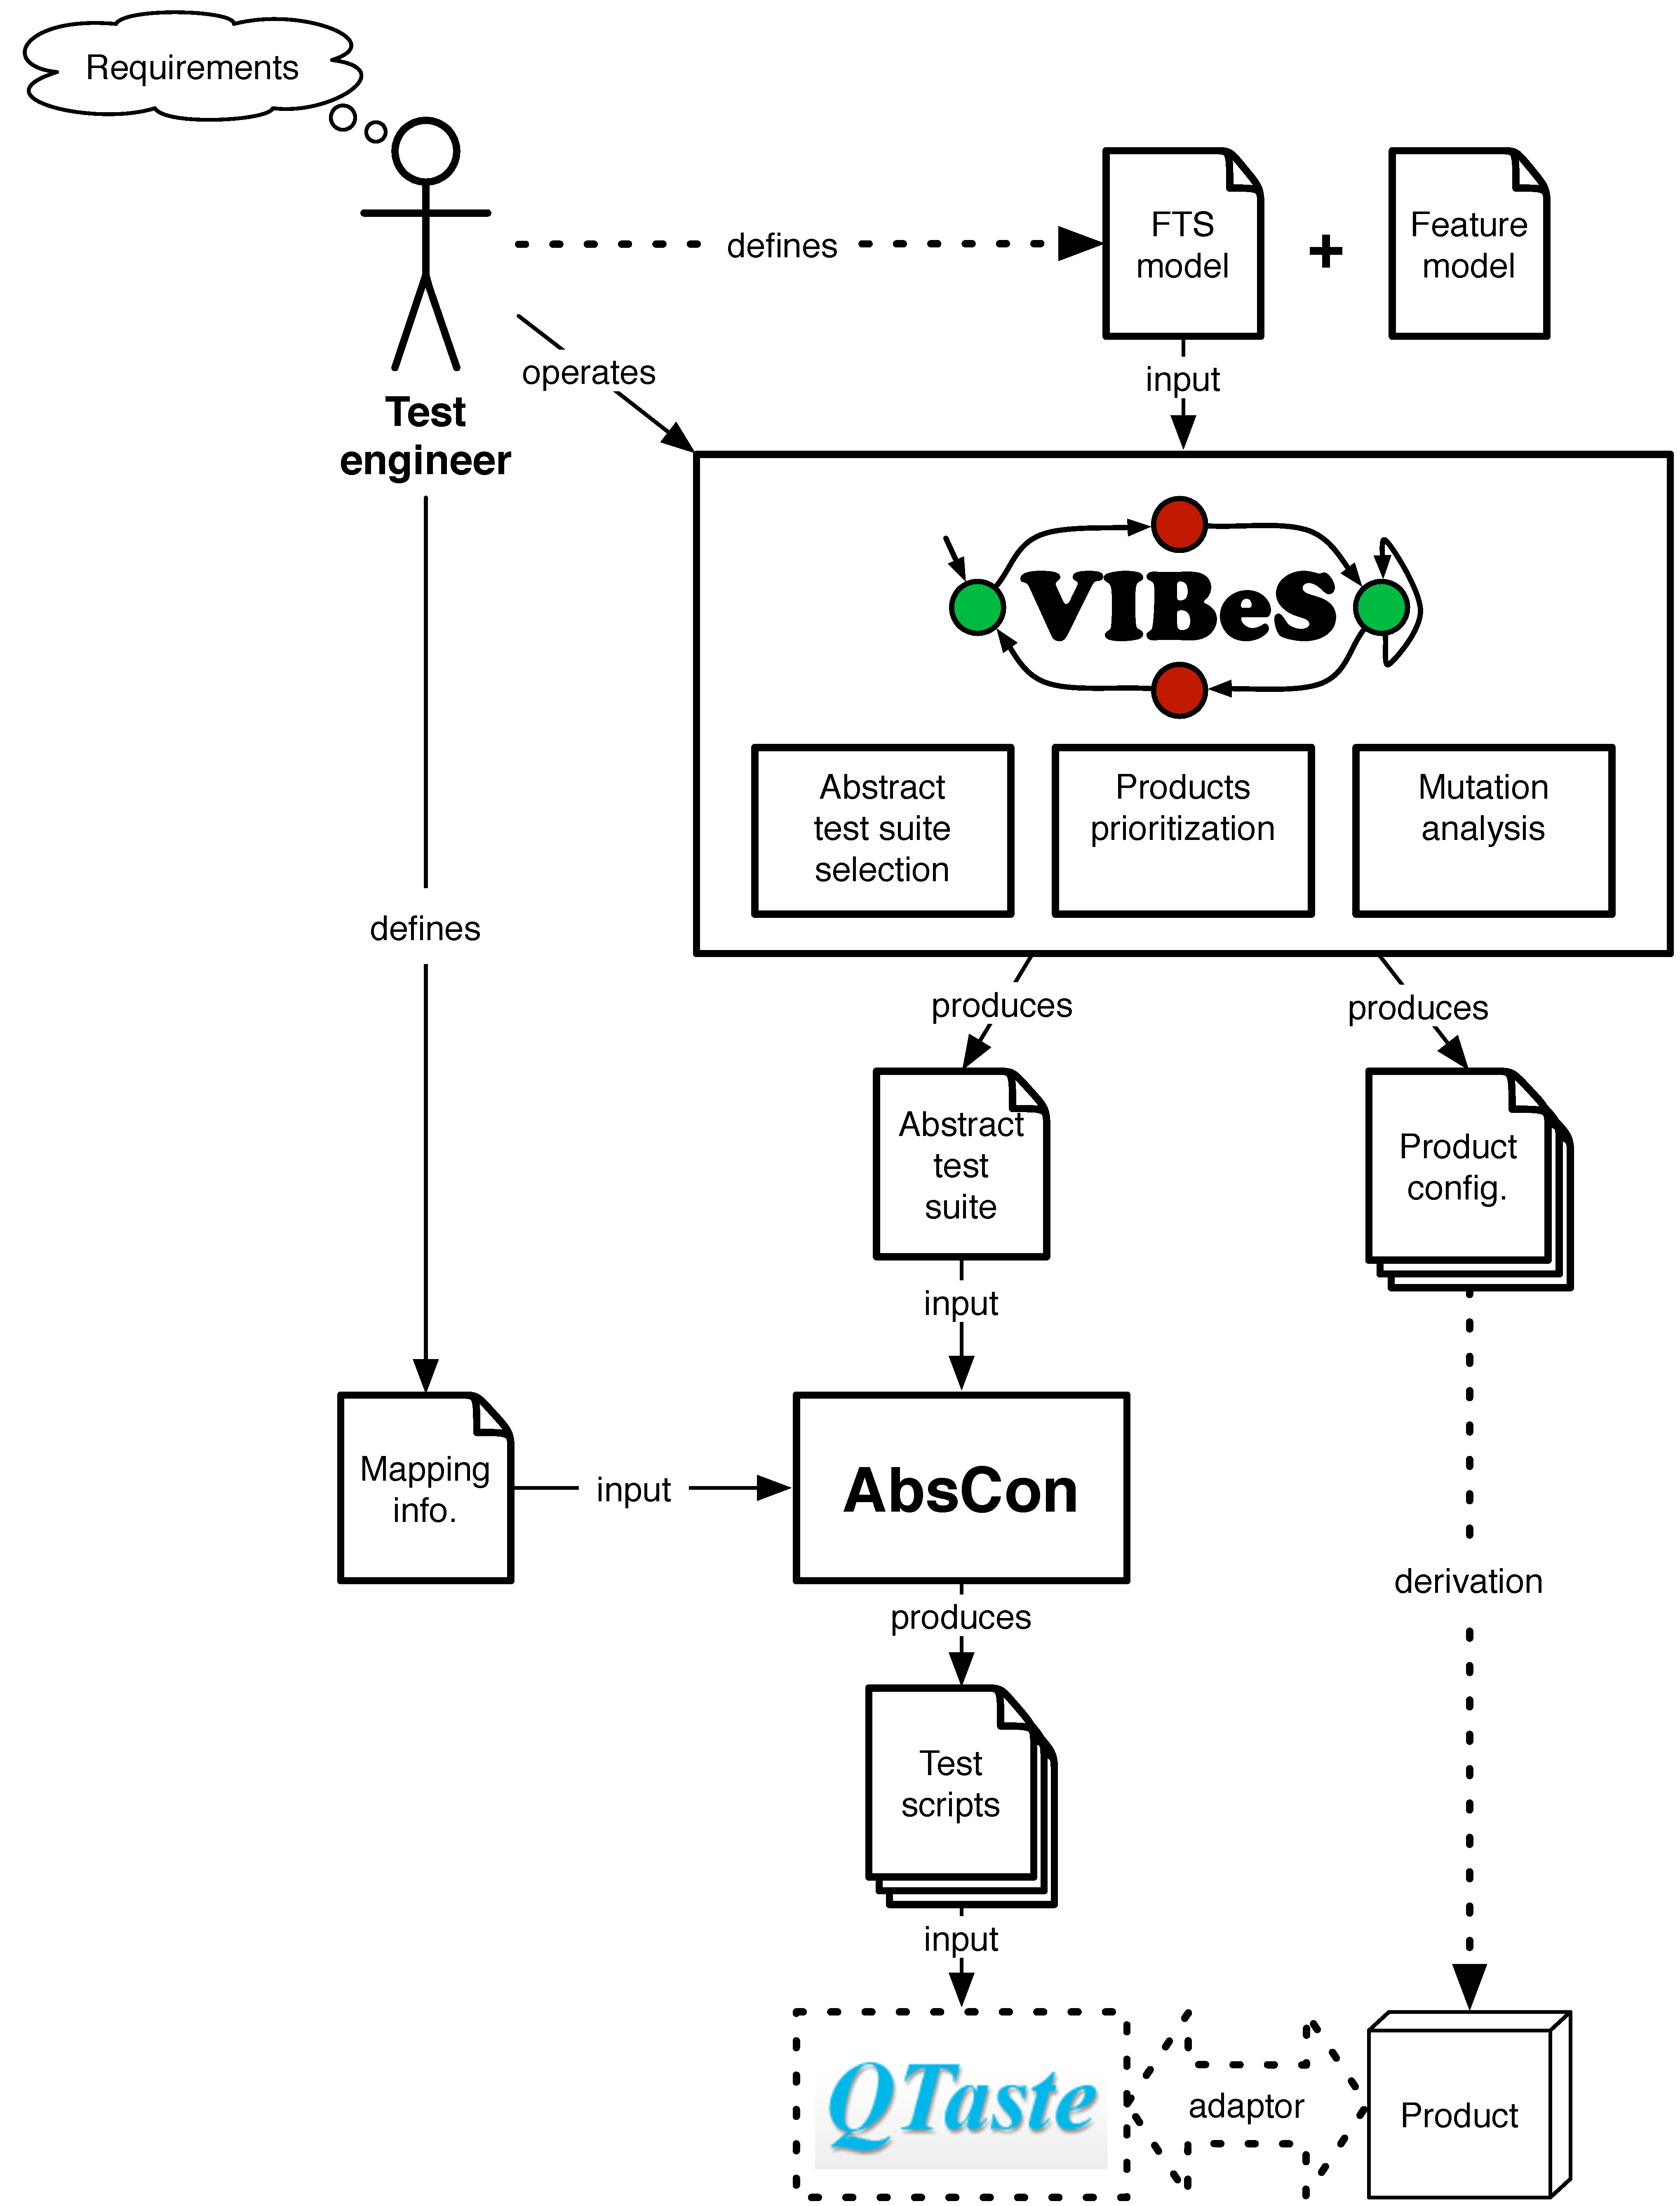
\includegraphics[width=110mm]{framework-overview}
	\caption{Behavioural SPL testing framework overview}
	\label{fig:frameworkoverview}
\end{figure}

\glsreset{VIBeS}

Figure \ref{fig:frameworkoverview} gives a general view of our framework. The test engineer, based on requirements, defines a FTS (and a feature model). This FTS serves as input to our tool: the \gls{VIBeS} framework. The tool is operated by the engineer to select a test suite, based on a selection criterion coming from the requirements. For instance, one may want to select a test suite that covers the states of the FTS or that contains test cases as dissimilar as possible. Based on this test suite, the engineer may prioritize the products to test, \eg by selecting the product that allows to execute as much test cases as possible, and assess the quality of the test suite using mutation analysis. 

\glsreset{AbsCon} \glsreset{QTaste}

Eventually, \gls{VIBeS} produces an \emph{abstract test suite}, with test cases representing sequences of actions from the FTS. This test suite is defined for the product line, which means that the abstract test cases, once concretized, may be executed by one or more products. The \emph{\gls{concretization}} is handled by the \gls{AbsCon} plugin, based on a \emph{mapping} provided by the test engineer. \gls{AbsCon} produces executable test scripts for the \gls{QTaste}, a test case management and execution system that uses an adaptor to handle communication with the product under test. The selection of the test cases to execute on the given product amongst all the test cases of the test suite is done in \gls{QTaste}, based on the list of abstract test cases executable by the selected product.

The different elements of Figure \ref{fig:frameworkoverview} are detailed, discussed, and evaluated in the next chapters: abstract test suite selection and product prioritization are presented in Chapter \ref{chap:coverage}; Chapter \ref{chap:mutation} discuss mutation analysis; Chapter \ref{chap:vibes} presents the implementation and usage of \gls{VIBeS}; and Chapter \ref{chap:concretization} details how concretization may be performed with \gls{AbsCon} to get test scripts executable by \gls{QTaste}. Elements in dashed lines in Figure \ref{fig:frameworkoverview} are out of the scope of this thesis and discussed in the next section.


%%%%%%%%%%%%%%%%%%%%%%%%%
\section{Uncovered aspects}
%%%%%%%%%%%%%%%%%%%%%%%%%

In this thesis, our main goal is to provide a framework to support the testing process. Software product line model-based testing is a complex task that involves many aspects, we identify the followings as out of the scope of this work.

%-------------------------------------
\subsection{Process management}
%-------------------------------------

\gls{VIBeS} is a toolbox that allows to perform various testing activities based on the requirements of the test engineer. In a software engineering context, those activities are organised in process \cite{swebok2014} that has to be managed and monitored. The definition of such product line model-based testing process falls out of the scope of this work.

%-------------------------------------
\subsection{Requirements definition}
%-------------------------------------

We assume that requirements are used both to define the FTS and the feature model, and the test suite selection criterion. The formalism used to define those requirements may take several forms: structured or semi-structured sentences \cite{cucumber}, goal modelling \cite{VanLamsweerde2008}, LTL formulas that the product line must satisfy \cite{Classen2013b}, \etc How those requirements are elicited  and formalised \cite{Bagheri2012,Niu2008,Metzger2014} is out of the scope of this work. We assume that the test engineer knows the requirements  when operating \gls{VIBeS}.

%-------------------------------------
\subsection{FTS model definition}
%-------------------------------------

In its implementation, \gls{VIBeS} allows to define FTSs using a Java DSL or with an XML file. The process used to define this \gls{FTS} model is out of the scope of this work. 

Model the detailed behaviour of the \gls{SPL} using an \gls{FTS} is intractable. Instead, the test engineer abstracts the behaviour to be able to run analysis on the model. This abstraction is done by defining abstract actions (\ie actions that represent one or more effective functions or methods calls) or by focusing on the subset of behaviour under test. As \glspl{FTS} may be used to express the semantic of other variability-aware behavioural languages \cite{Cordy2014}, one may also use an abstract modelling language: \eg FORML \cite{Shaker2012a,Shaker2012}. In such a case, we assume that a bidirectional mapping can be defined between the abstract modelling language and FTS.

%-------------------------------------
\subsection{Feature model definition}
%-------------------------------------

We assume that the feature model used with the \gls{FTS} is a boolean feature model that may be translated to a \gls{CNF} formula \cite{Batory2005,Schobbens2007}. As for \glspl{FTS}, the definition and the formalism used to define this feature model are out of the scope of this work. Considering non-boolean feature models requires to use constraint solvers other than \gls{SAT} or \gls{BDD} solvers, and to adapt \glspl{FTS}' feature expressions to take non-boolean types into account.

%-------------------------------------
\subsection{Product derivation}
%-------------------------------------

\gls{VIBeS} produces a set of product configurations to test. This set is represented as a set of boolean assignments of the feature model. The derivation process of the actual product (in dashed lines in Figure \ref{fig:frameworkoverview}) is out of the scope of this work. This derivation may take several forms and may be automated or not \cite{Pohl2005}.

%-------------------------------------
\subsection{Test scripts execution}
%-------------------------------------

Test scripts management, covering executions of the scripts and reporting, is handled by \gls{QTaste}. \gls{QTaste} is an industrial test environment that provides functionalities to execute test scripts using an adaptor to manipulate the product under test. More details about \gls{QTaste} are provided in Chapter \ref{chap:concretization}.


%%%%%%%%%%%%%%%%%%%%%%%%%%%%%%%%%%%
\section{Wrap up}
%%%%%%%%%%%%%%%%%%%%%%%%%%%%%%%%%%%

This chapter presents an overview as well as the limitations of our behavioural model-based product line testing framework. We assume connected \glspl{FTS} and boolean \glspl{feature model} as inputs. The different elements of the framework are detailed in the next chapters.


\chapter{Case studies}
\label{chap:casestudies}

We present in this chapter the different case studies used along the thesis. We consider models from different sources with varying size. 
Our models are: 
%
the soda vending machine model (\textit{S. V. Mach.}) in Section \ref{sec:casestudy:svm};
%
the mine pump (\textit{Mine\-pump}) in Section \ref{sec:casestudy:minepump};
%
the WordPress models (\textit{AGE-RR}, \textit{AGE-RRN}, \textit{Elsa-RR}, and \textit{Elsa-RRN}) in Section \ref{sec:casestudy:wordpress};
%
the Claroline website (\textit{Claroline}) in Section \ref{sec:casestudy:claroline};
%
and the random models (\textit{Random} \textit{1-4}) in Section \ref{sec:casestudy:random}.
%
We compare the models characteristics in Section \ref{sec:casestudy:characteristics} and define the threats to validity linked to the selection of our case studies in Section \ref{sec:casestudy:threats}.


%%%%%%%%%%%%%%%%%%%%%%%%%%%%%%%%%%%
\section{Soda vending machine}
%%%%%%%%%%%%%%%%%%%%%%%%%%%%%%%%%%%

\label{sec:casestudy:svm}

\begin{figure}[t]
	\centering
	\subbottom[Feature model]{
		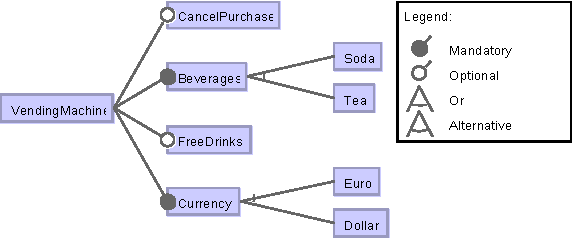
\includegraphics[width=95mm]{svm-fm}
		\label{fig:svmfm}
	}	
	\subbottom[Featured transition system]{
		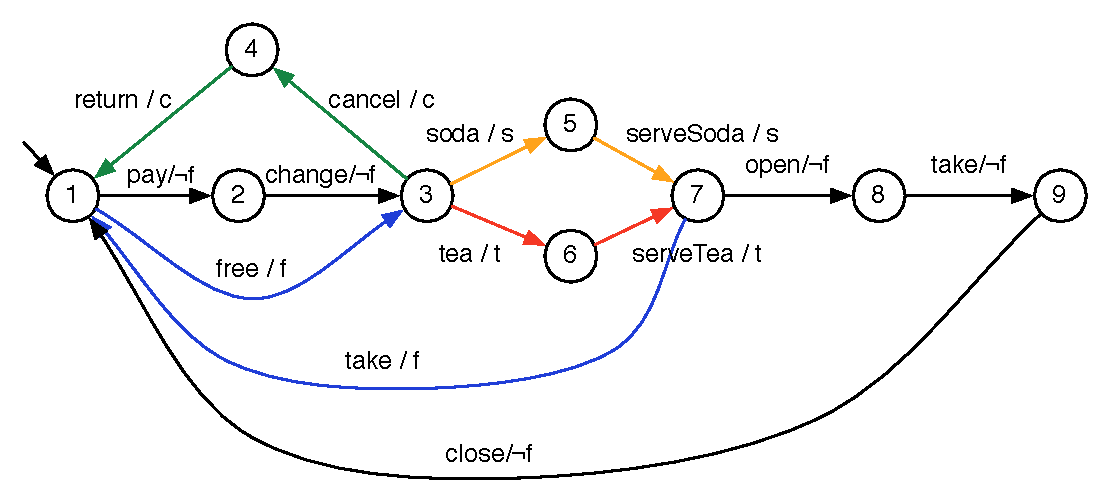
\includegraphics[width=105mm]{svm-fts}
		\label{fig:svmfts}
	}
	\caption{Soda vending machine}
\end{figure}

The \gls{soda vending machine} SPL is a classical beverage vending machine described by Classen \etal \cite{Classen2013b}. The \gls{feature model} is presented in Figure \ref{fig:svmfm}: it sells soda ($s$) or tea ($t$) in euro or dollar, may offer free drinks ($f$), and optionally allows to cancel a purchase ($c$). The \gls{FTS} describing the behaviour of the SPL is presented in Figure \ref{fig:svmfts} (for readability, the feature names have been shortened): the user either pays or chooses a free drink (if feature $f$ has been selected); he may cancel its purchase (if feature $c$ has been selected); he chooses a beverage, allowed by the selected features; and gets his beverage directly (if feature $f$ has been selected) of after opening the machine (otherwise).


%%%%%%%%%%%%%%%%%%%%%%%%%%%%%%%%%%%
\section{Card payment terminal}
%%%%%%%%%%%%%%%%%%%%%%%%%%%%%%%%%%%

\label{sec:casestudy:cpterminal}

\begin{figure}
	\centering
	\subbottom[Feature model]{
		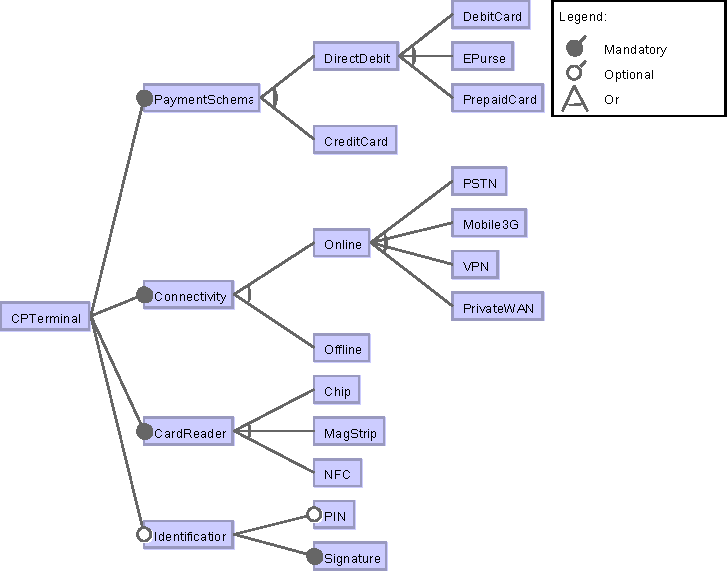
\includegraphics[width=110mm]{cpterminal-fm}
		\label{fig:cpterminalfm}
	}	
	\subbottom[Featured transition system]{
		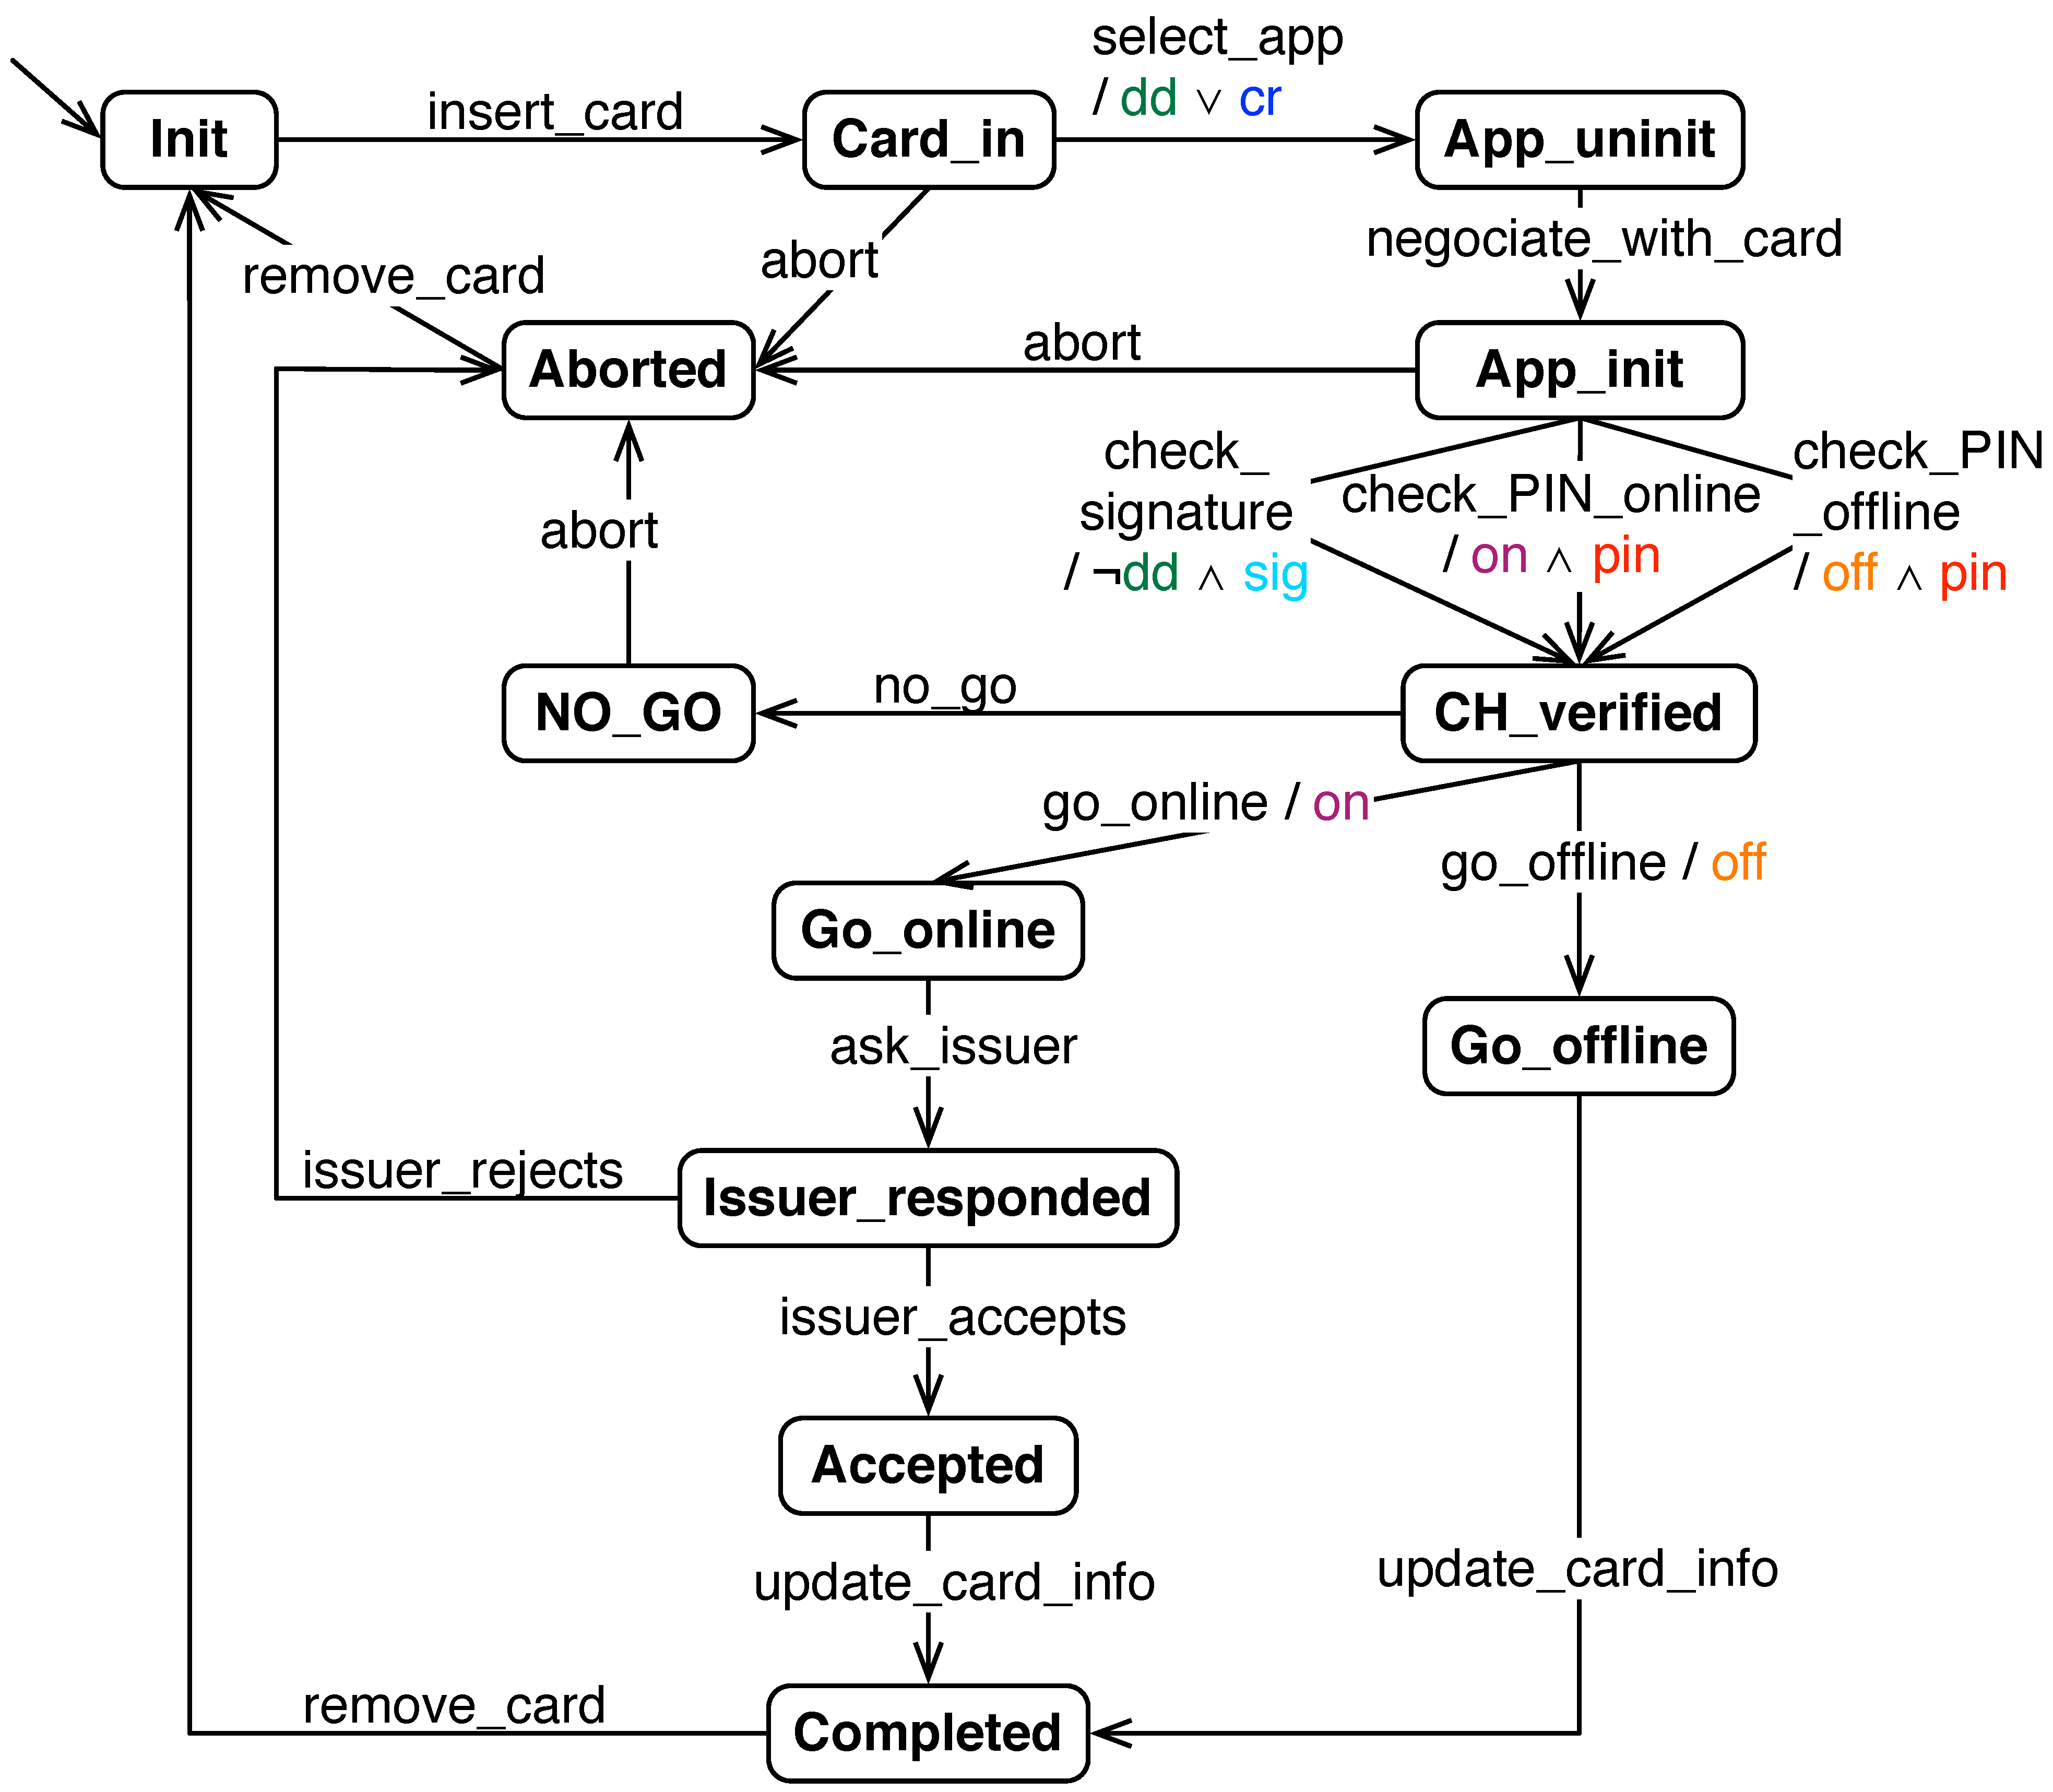
\includegraphics[width=85mm]{cpterminal-fts}
		\label{fig:cpterminalfts}
	}
	\caption{Card payment terminal}
\end{figure}

Figure \ref{fig:cpterminalfm} presents the \gls{feature model} of a card payment terminal manually defined using Eurocard-Mastercard-Visa (EMV) specification document \cite{EMVCo2011}. This machine accepts card payment with a given payment schema (direct debit and/or credit card). It works online, using one or more connectivity option, or offline with the card payment service. Cards are read using a chip, the magnetic strip, or near field contact (NFC); and card owner may be authenticated using signature and optionally PIN code.

The FTS in Figure \ref{fig:cpterminalfts} presents the behaviour (we want to test) of the card payment terminal (minus one technical intermediate state) to processes a payment. First, the Card Holder (CH), \ie the user, inserts his card in the terminal. If the card is a direct debit ($dd$) or a credit card ($cr$), the terminal will proceed the initialisation of the transaction. In this version of the product line, the card holder must always identify himself using either: his signature if the card is not a direct debit card and if the terminal supports the signature identification ($sig$); or his secret \gls{PIN} if the terminal supports PIN identification ($pin$), which may be checked online ($on$) or offline ($off$) with the transaction processor company. If the identification succeeds, the terminal will proceed online or offline to the payment, otherwise, the transaction is aborted. Whether the transaction succeeds or not, the card holder removes his card from the terminal at the end of the process.


%%%%%%%%%%%%%%%%%%%%%%%%%%%%%%%%%%%
\section{Minepump}
%%%%%%%%%%%%%%%%%%%%%%%%%%%%%%%%%%%

\label{sec:casestudy:minepump}

\begin{figure}
	\centering
	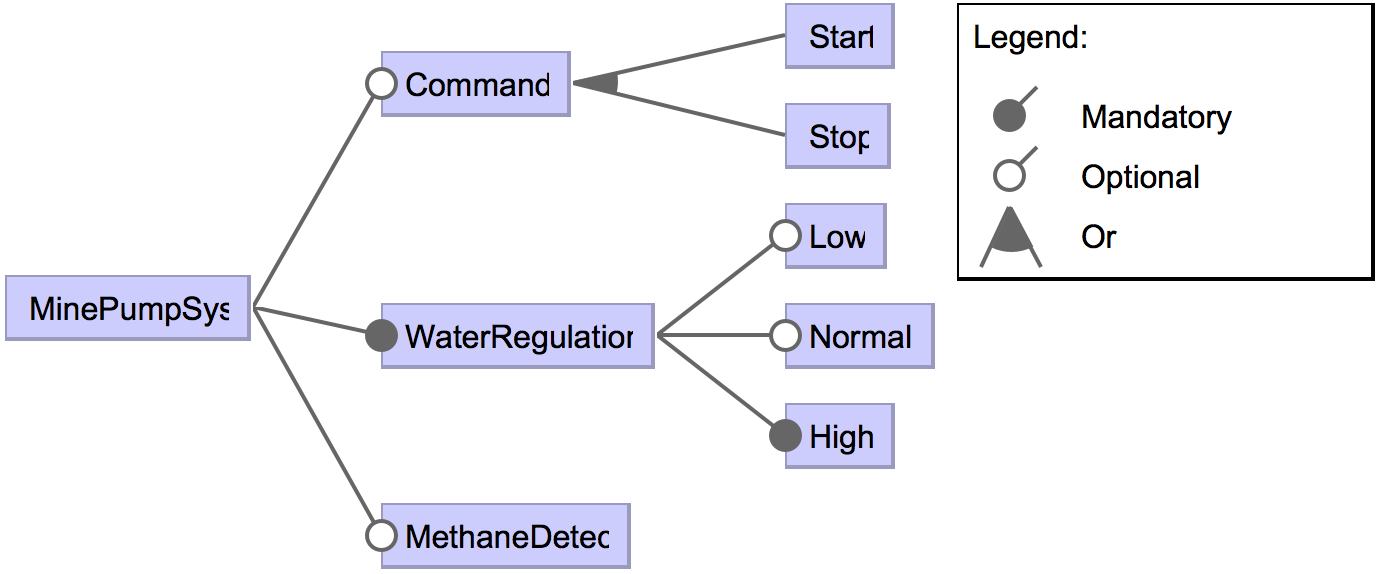
\includegraphics[width=95mm]{minepump-fm}
	\caption{Minepump feature model}
	\label{fig:minepumpfm}
\end{figure}

The Minepump model \cite{Classen2010b} represent a product line of pumps designed to keep a mine shaft clear of water and (optionally) avoid the danger of a methane explosion. Figure \ref{fig:minepumpfm} presents the feature model of the SPL. A pump has a water regulator that can detect the level of water in the shaft. It may be equipped with a methane detector and a command interface allowing to manually start and stop the pump. The FTS describing the behaviour of the pumps has 25 states and 41 transitions. 


%%%%%%%%%%%%%%%%%%%%%%%%%%%%%%%%%%%%%%%%%%%%%%%%%%%%%%%%%%%%%%
\section{Sferion\texttrademark landing symbology function}
%%%%%%%%%%%%%%%%%%%%%%%%%%%%%%%%%%%%%%%%%%%%%%%%%%%%%%%%%%%%%%

\label{sec:casestudy:sferion}

\begin{figure}
	\centering
	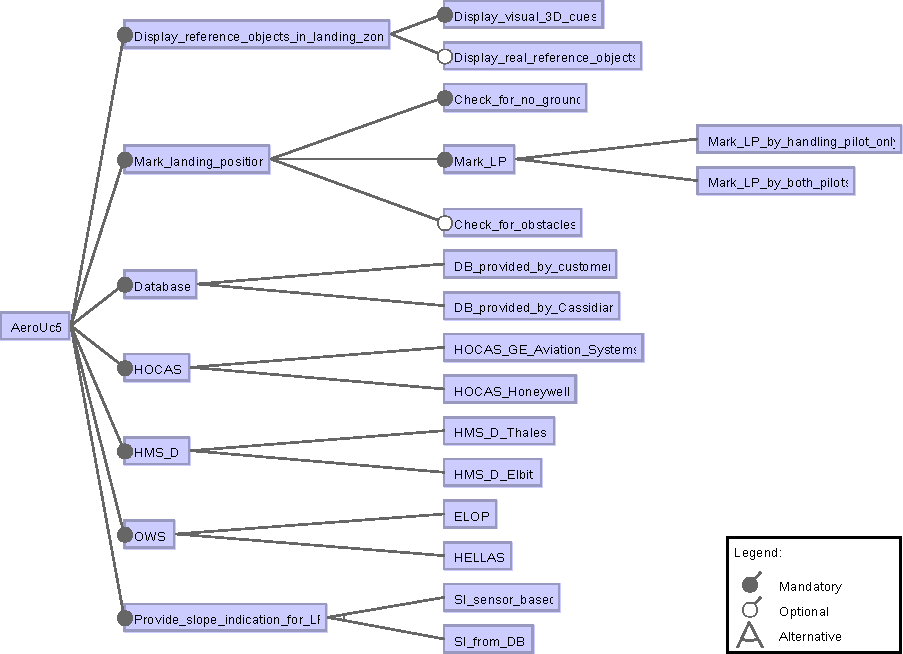
\includegraphics[width=0.98\textwidth]{aerouc5-fm}
	\caption{Sferion\texttrademark landing symbology function feature model}
	\label{fig:aerouc5fm}
\end{figure}

Sferion\texttrademark ~is an industrial situational awareness suite for helicopters flying in degraded visual environments \cite{Devroey2015a,sferion,Samih2014c}. The landing symbology function supports the pilot during the landing approach by marking the intended landing position on ground using a head-tracked Helmet Mounted Sight and Display (HMS/D) and Hands On Collective And Stick (HOCAS). Depending on the selected feature, the landing may be marked by the handling pilot only or by bots pilots. The spatial awareness is enhanced during the final landing approach by displaying 3D conformal visual cues on the helmet with optionally real reference of the object. The ground (and optionally obstacles) in the landing zone are detected and classified using a real-time Obstacle Warning System (OWS). Depending on the customer and the helicopter platform, the landing symbolog1y function may have different features (Figure \ref{fig:aerouc5fm}) selected: \textit{ELOP} or \textit{HELLAS} sensors for the \textit{OWS}; \textit{SI\_sensor\_based} or \textit{SI\_from\_DB} as slope indication provider for landing position; the Thales or Elbit HMS/D; the HOCAS from Honeywell or from Aviation Systems inc.; a database provided by the helicopter platform or a Cassidian database.

The models have been designed by engineers using MaTeLo \cite{matelo} tool, OVM and Matelo Product Line Management (MPLM) \cite{Samih2014b}. They have originally been presented by Samih et al. \cite{Samih2014c}. MaTeLo supports the description of statistical usage models by using hierarchical Markov chains. MaTeLo's usage model is a \gls{DTMC}, where the nodes represent the major states of the system and the transitions are labelled with the actions or operations of the SUT with their probability to be fired. In a DTMC, the transitions are tagged with a probability representing the likelihood, when we are in the starting state, to execute the transition, and the action performed when the transition is executed. Each action is associated with zero, one or more requirements. The variability is described using OVM (Orthogonal Variability Model), each variation point is associated to zero, one or more requirement(s). The mapping, encoded in MPLM, between the variation points and the usage model transitions is made through the requirements. MPLM and MaTeLo tools support the product-based test derivation approach.

We encoded the Sferion\texttrademark ~landing symbology function models using our formalisms: the usage model has been flattened to remove hierarchy (by hand in 1/2 day); the OVM model has been translated to a feature model (by hand in 1/2 day); and the mapping between features and behaviour has been encoded using an FTS, generated from the MaTeLo usage model, the OVM model and the MPLM mapping model (in 1 day).


%%%%%%%%%%%%%%%%%%%%%%%%%%%%%%%%%%%%%%%%%%%%%%%%%%%%%%%%%%%%%%
\section{WordPress, an open-source CMS}
%%%%%%%%%%%%%%%%%%%%%%%%%%%%%%%%%%%%%%%%%%%%%%%%%%%%%%%%%%%%%%

\label{sec:casestudy:wordpress}

WordPress \cite{wordpress} is a popular open-source \acrfull{CMS} used by more than 60 million websites \cite{Colao2012}. It includes a plugin architecture and a template system, allowing one to modify its behaviour by adding new functionalities (\ie plugins), or the rendering of the website (\ie themes), respectively. In February 2017, the WordPress database (\url{https://wordpress.org/}) counted 48,898 plugins and 4,462 (latest) themes. 

We reverse-engineered the feature models and the FTSs of two WordPress instances, AGE and Elsa portals, based on their Apache webserver log file. The \gls{AGE} website (\url{http://www.age-namur.be}) is the portal of the general student assembly of the University of Namur. It uses a dedicated WordPress instance and provided us a log file with 1,285,592 entries from May 2013 to March 2014. The European Law Students' Association (Elsa) of Louvain-la-Neuve  (\url{http://elsa-lln.be}) also uses a dedicated WordPress instance and provided us a log with 48,823 entries from February 2014 to the end of April 2014.

%---------------------------
\subsection{Feature model} 
%---------------------------

\label{subsec:wordpress:fm}

\begin{figure}
\centering
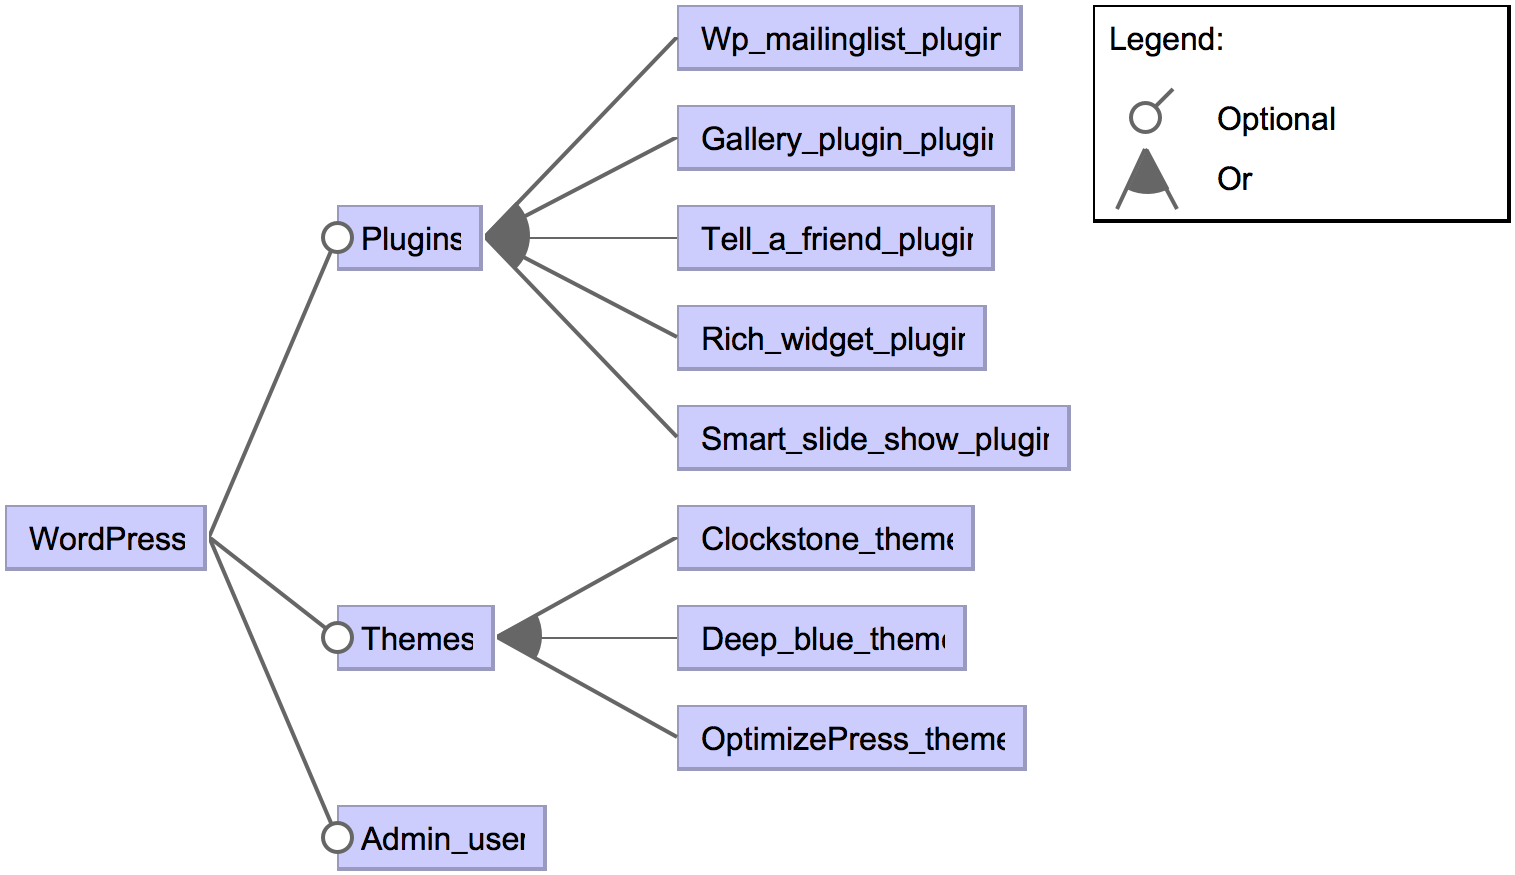
\includegraphics[width=100mm]{wordpress-simplified}
\caption{Simplified WordPress feature model}
\label{fig:wordpressfm}
\end{figure}

Our WordPress feature model has 3 optional core features: \textit{Plugins}, \textit{Themes}, and \textit{Admin\_user}. One configuration (\ie product) of the feature models represents the minimal instance needed to play a test suite. The \textit{Admin\_user} feature will be selected only if a test case requires to access the administration pages. 

To identify the plugins and themes used in the instances, we analysed the Apache webserver log entries. Each time an HTTP request is addressed to the server, one entry is created in the log file with the following format \cite{apacheserver}: the IP address of the visitor sending the request; a login if the visitor is identified on the system; the date and time of the request; the HTTP request itself, beginning with  GET, POST, \etc, followed by a URL and the protocol version; the status code sent back to the client; the size of the object returned to the client; the website the client reports having been referred from; and finally the information on the client's browser. For instance, a request to the \texttt{index.php} page of the WordPress instance from a Mozilla Firefox navigator will add the following entry in the log file:
%
\begin{lstlisting}[basicstyle=\footnotesize\ttfamily,frame=single,breaklines,columns=flexible]
66.155.40.250 - - [08/Nov/2013:11:38:11 +0100] "GET /index.php?p=potins&action=aimepas&id=135 HTTP/1.1" 200 708388 "-" "Mozilla/5.0 (Windows NT 6.1; WOW64; rv:25.0) Gecko/20100101 Firefox/25.0"
\end{lstlisting}
%
Plugins and themes resources are placed in specific folders on the webserver. This allows us to filter the URL of the log entries using the following regular expressions:
\begin{itemize}
\item \verb?.*/wp-content/plugins/([^/]+)/.*? to detect access to a plugin resource;
\item \verb?.*/wp-content/themes/([^/]+)/.*? to detect access to themes resources;
\item \verb?.*/wp-admin/.*? to detect that an administration page has been used.
\end{itemize}
The names of the plugins and themes appears right after the \texttt{plugins/} and \texttt{themes/} part of the URL (matched by the \verb?([^/]+)? part of the regular expression). Since the logs have been anonymized, we do not have the identification of the users and rely on the last regular expression to detect administrator accesses to the WordPress instance.

We ended up with two feature models: one with 45 features for the AGE WordPress instance, and one with 70 features for the Elsa WordPress instance. Figure \ref{fig:wordpressfm} presents a simplified version of the Elsa WordPress instance (AGE instance follows the same pattern).
The root feature \textit{WordPress} is decomposed in three optional sub-features: \textit{Admin\_user}, \textit{Themes}, and \textit{Plugins}. Each plugin or theme (resp.) appearing in a log entry will be a sub-feature of the \textit{Plugins} or \textit{Themes} (resp.) feature. 

Another approach to build the feature model would have been to mine the plugins and themes repository of WordPress. This would give a much larger feature model: more than 50,000 features. Since we are in behavioural model-based context, we seek to find incorrect behaviour in the product line. This incorrect behaviour may be caused by feature interaction or may have another root cause (\eg an error in the source code introducing faults in all the products). In order to select our test cases, we need a behavioural model of the SPL, which is derived from the Apache  Web server log. In this context, considering all the WordPress plugins and themes in the feature model has little meaning since only the behaviour of the plugins and themes activated in the running WordPress instances (appearing in the log) will appear in the behavioural model. This is why we consider only those plugins and themes as relevant for testing and add them in the feature models. 

Similarly, S\'anchez \etal \cite{Sanchez2013a,Sanchez2017} used a white box testing approach to test the Drupal CMS. They rely on documentation, source code, issue tracking system, and Git versioning repository to reverse engineer the system's feature model. Stress is put on product selection, whereas we focus on behaviour selection (at the product line level) in a black box approach. 

%---------------------------------------
\subsection{Featured transition system} 
%---------------------------------------

\label{subsec:wordpress:fts}

We reverse engineered the FTSs of the AGE and Elsa WordPress instances using a 2-gram (bigram) inference method \cite{Sprenkle2011a,Sprenkle2013}. This method uses a set of \emph{user sessions} (\ie sequences of HTTP requests) to generate a navigational model of a website. In the generated FTS, the states represents the last user request and the transitions represents the sequence between two requests. Transitions leading to a request identified as part of a plugin or a theme, or as accessible only by an administrator (using the regular expressions from the previous section) are labelled with the corresponding feature expression.

The $n$-gram inference method has been proposed by Sprenkle \etal \cite{Sprenkle2011a,Sprenkle2013} and used to test website in a black box fashion. They experiment the inference with different configurations and values of $n$ greater than 2 and found out that a small $n$ allows better diversity in the behaviours (ending up in more diverse test cases), and requires less sessions to reach growth stability of the model. Small $n$ also simplifies the generation and results in a more compact model. This motivates our choice to select 2-gram for the inference.


\paragraph{User sessions:}
%--------------------------

One user session corresponds to a sequence of HTTP requests, representing the sequence of pages consulted by the user. User sessions can be extracted from the Apache webserver log by grouping entries with the same IP address (assuming that one IP corresponds to one user) and logged within a same time frame. This means that two entries in a user session may not be distant by more than a maximal timeout (we arbitrarily choose to set a timeout of 3 minutes). If the timeout is reached, the next entry will be the first of a new user session.

To build the user sessions, we only consider some relevant elements of the HTTP request \cite{Sprenkle2013}. This allows to group behaviour of various users to identify common usage scenarios. Amongst the possible group of elements, we considered:
\begin{itemize}
\item \emph{Request type} and \emph{Resource} (RR), which uses the type of HTTP request (\eg PO\-ST or GET) and the resource name (\eg \texttt{/index.php}) for a user session element;
\item \emph{Request type}, \emph{Resource}, and \emph{parameters Names} (RRN), which also uses the HTTP request type and the name of the resource, but also the name of the parameters in the resource (\eg \verb|?p=&action=&id=|).
\end{itemize}

 
\paragraph{Bigram inference:}
%---------------------------

\begin{algorithm}[h]
	\KwIn{\textit{sessions}: the set of non empty user sessions}
	\KwOut{\textit{fts}: an FTS representing a navigational model}
	\Begin{
		$S = \{ s_0 \}$; $\Act = \emptyset$; $\trans = \emptyset$; $i=s_0$; $\gamma= \rightarrow (\rightarrow \bot)$ \; \nllabel{algo:bigram:line:init}
		\For{\textit{sess} $\in$ \textit{sessions} \nllabel{algo:bigram:line:mainloop}}{
			\textit{S.add(sess[0])}\; \nllabel{algo:bigram:line:sessioninit1}
			\textit{Act.add(req(sess[0]))} \; \nllabel{algo:bigram:line:sessioninit2}
			\textit{tr} = $s_0 \xrightarrow{\mathit{req}(\mathit{sess}[0])} \mathit{sess}[0]$\; \nllabel{algo:bigram:line:sessioninit3}
			\textit{trans.add(tr)}\; \nllabel{algo:bigram:line:sessioninit4}
			$\gamma = fLabels(\gamma, tr) $\; \nllabel{algo:bigram:line:sessioninit5}
			\For{$i \in [1;sess.size[$ \nllabel{algo:bigram:line:sessionloop}}{
				\textit{S.add(sess[i])}\;  \nllabel{algo:bigram:line:addstate}
				\textit{Act.add(req(sess[i]))}\; \nllabel{algo:bigram:line:addaction}
				\textit{tr} = \textit{sess[i-1]} $\xrightarrow{\mathit{req}(\mathit{sess}[i])}$ \textit{sess[i]}\; \nllabel{algo:bigram:line:addtransition}
				\textit{trans.add(tr)}\; 
				$\gamma$ = \textit{fLabels(}$\gamma$\textit{, tr, sess[i])} \; \nllabel{algo:bigram:line:addlabels}
	  		}
			$Act.add(req(s_0))$\; 
			$trans.add(sess[sess.size - 1] \xrightarrow{req(s_0)} s_0)$\;	 \nllabel{algo:bigram:line:addfinaltransition}
	  	}		
	  	$\fts = (S, \Act, \trans, i, \mathit{fm}(\mathit{sessions}), \gamma)$\; \nllabel{algo:bigram:line:ftsinit}
  		\Return $fts$\;
	}
	\caption{WordPress bigram FTS building}
 \label{algo:bigram}
\end{algorithm}

Using a bigram inference, the next state only depends on the current state of the system. As a consequence, user session entries are considered two by two: the last user request, which is the current state, and the next request of the user, which is the next state of the system.

Algorithm \ref{algo:bigram} presents the bigram inference of the FTS for a WordPress instance, based on a set of user sessions. The elements of the FTS are initialised at line \ref{algo:bigram:line:init}. For each session (line \ref{algo:bigram:line:mainloop}), the sequence of requests enriches the model: sessions starts from a virtual state $s_0$ and the first sequence adds a transition from this state to a new state corresponding to the first element of the sequence (lines \ref{algo:bigram:line:sessioninit1} to \ref{algo:bigram:line:sessioninit3}); transitions are labelled with actions representing the request of another page (lines \ref{algo:bigram:line:sessioninit2} and \ref{algo:bigram:line:addaction}); and each new transition is labelled with a feature expression (lines \ref{algo:bigram:line:sessioninit5} and \ref{algo:bigram:line:addlabels}).
%
This feature expression corresponds to the conjunction of the previous feature expression if there is one or true otherwise, and the  name of a plugin, a theme, or the administrator user if the requested resource matches one of the corresponding regular expression from section \ref{subsec:wordpress:fm}. Function \textit{fLabels} enriches $\gamma$ definition, based on its previous definition and the given transition. 
%
This process iterates for each request in the sequence (line \ref{algo:bigram:line:sessionloop}), the starting state corresponding to the target state of the previous iteration. Finally, each sequence terminates by a special action \textit{req}$(s_0)$, resetting the system, and ends in the virtual state $s_0$ (line \ref{algo:bigram:line:addfinaltransition}). The algorithm returns an FTS with the inferred navigational model and a feature diagram build using the method described in section \ref{subsec:wordpress:fm} (line \ref{algo:bigram:line:ftsinit}). We implemented Algorithm \ref{algo:bigram} in an open source tool: Yet Another Model Inference tool (YAMI), available at \url{https://github.com/xdevroey/yami}.

We built four FTSs: two using Request type and Resource (RR) parts of the URLs as sequence elements in the user sessions (\emph{AGE-RR} with 772 states and 6,639 transitions, and \emph{Elsa-RR} with 384 states and 1,214 transitions), and two using Request type, Resource, and parameter Names (RRN) parts of the URLs (\emph{AGE-RRN} with 1,101 states and 10,960 transitions, and \emph{Elsa-RRN} with 615 states and 1,771 transitions). The process took 3 seconds to process the 3,964 sessions of the Elsa models (average session size=9.57, $\sigma$=46.73) and 54 second to build the 147,173 sessions of the AGE models (average session size=5.10, $\sigma$=61.04) on a Ubuntu Linux machine (Linux version 3.13.0-65-generic, Ubuntu 4.8.2-19ubuntu1) with an Intel Core i3 (3.10GHz) processor and 4GB of memory.


%%%%%%%%%%%%%%%%%%%%%%%%%%%%%%%%%%%%%%%%%%%%%%%%%%%%%%%%%%%%%%
\section{Claroline, a course management system}
%%%%%%%%%%%%%%%%%%%%%%%%%%%%%%%%%%%%%%%%%%%%%%%%%%%%%%%%%%%%%%

\label{sec:casestudy:claroline}

The instance of Claroline at University of Namur\footnote{\url{http://webcampus.unamur.be}} is the main communication channel between students and lecturers and is used by approximately 7000 users. Students may register to courses and download documents, receive announcements, submit their assignments, perform online exercises, \etc 
Claroline is a configurable system \cite{Cohen2008}. Contrary to classical SPL, the selection of the features does not occur during the development of the software (at design time in a SPL lifecycle) \cite{Pohl2005}, but during its execution (at runtime). Thus, a product can dynamically evolve while the system is running: this requires the system architecture to be able to accommodate evolutions, by following plugin-based or component-based architectural styles. Thanks to the versatility of the feature concept \cite{Classen2008}, it is possible to represent design time and runtime product using the same formalism (FM), as product semantics is ultimately given through the mapping with the FTS. In the Claroline case, features represent installation parameters. A product represents a running Claroline instance with a minimal set of data.  

%---------------------------
\subsection{Feature model} 
%---------------------------

\label{sec:casestudy:claroline:fm}

\begin{figure}
\centering
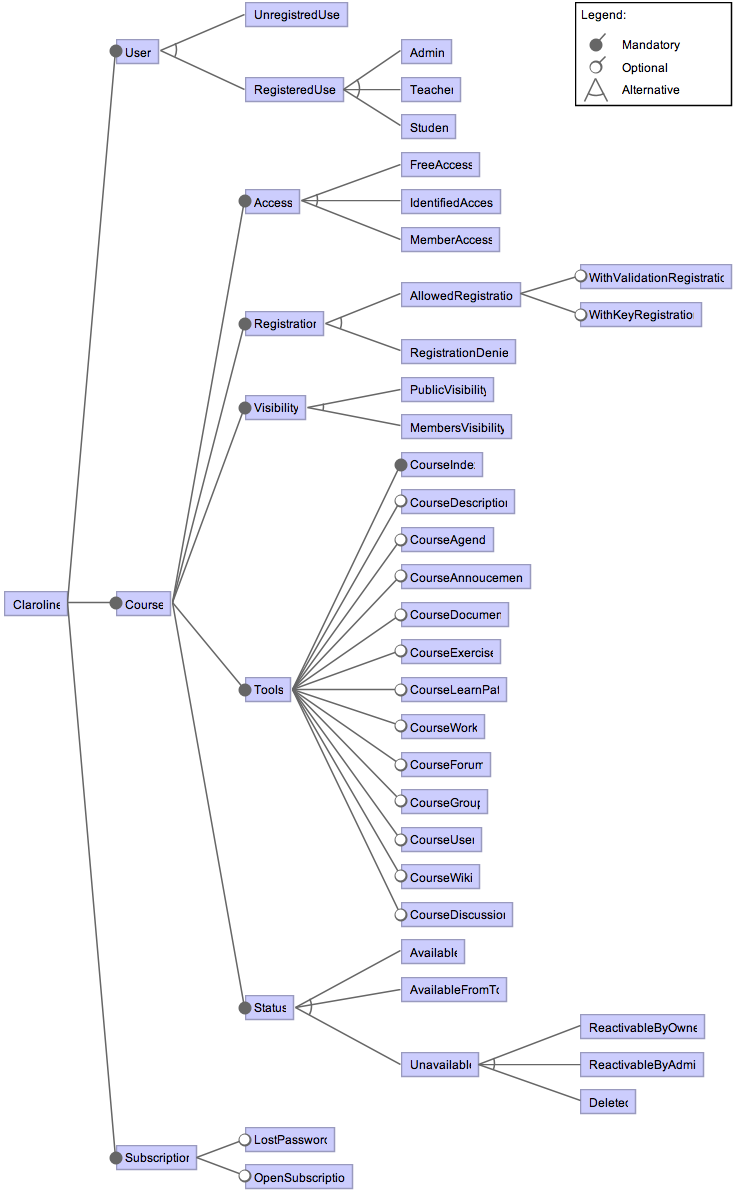
\includegraphics[height=0.95\textheight]{claroline-fm}
\caption{Claroline feature model}
\label{fig:clarolinefm}
\end{figure}

We manually built the \gls{FM} from the Claroline documentation and from inspection of a locally installed Claroline instance (Claroline 1.11.7) in approximately 3 days (by one person). The FM in Fig. \ref{fig:clarolinefm} (additional constraints have been omitted) describes Claroline with three main features: \textit{User}, \textit{Course} and \textit{Subscription}. \textit{Subscription} may be open to everyone (\textit{opt} \textit{OpenSubscription}) and may have a password recovery mechanism (\textit{opt} \textit{LostPassword}). 

\textit{User} corresponds to the different possible user types provided by default with a basic Claroline installation: unregistered users (\textit{UnregisteredUser}) who may access courses open to everyone and registered users (\textit{RegisteredUser}) who may access different functionalities of the courses according to their privilege level (\textit{Student}, \textit{Teacher} or \textit{Admin}). The last main feature, \textit{Course}, corresponds to the page dedicated to a course where students and teacher may interact.

A course has a status (\textit{Available}, \textit{AvailableFromTo} if the course is available only during a specific period, or \textit{Unavailable}), may be publicly visible (\textit{PublicVisibility}) or not (\textit{MembersVisibility}), may authorize registration to identified users (\textit{AllowedRegistration}) or not (\textit{RegistrationDenied}) and may be accessed by everyone (\textit{FreeAccess}), identified users (\textit{IdentifiedAccess}) or members of the course only (\textit{MembersAccess}). Moreover, a course may have a list of tools (\textit{Tools}) used for different teaching purposes, \eg an agenda (\textit{opt} \textit{CourseAgenda}), an announcement panel (\textit{opt} \textit{CourseAnnoucements}), a document download section where lecturers may post documents and students may download them (\textit{opt} \textit{CourseDocument}), an online exercise section (\textit{opt} \textit{CourseExercise}).
 
Since we are in a testing context, one product of the FM does not represent a complete Claroline instance, but the minimal instance needed to play a test suite. Basically, it maps to a Claroline instance with one particular user and one particular course.
This is similar to the technique presented by Segura et al. \cite{Segura2014} used to represent the testing entry domain of a e-commerce web site.
In order to represent a complete Claroline instance (with all its users and courses), we need to introduce cardinalities \cite{Michel2011} on the \textit{User} and  \textit{Course} features in order to have multiple users and multiple courses. Eventually we obtained a FM with 44 features.

%---------------------------------------
\subsection{Featured transition system} 
%---------------------------------------

\label{sec:casestudy:claroline:fts}

Regarding the \gls{FTS}, we also used a bigram inference method (see section \ref{subsec:wordpress:fts}) on a 5.26 Go Apache webserver log with 45,210,987 entries from January 2013 to September 2013. Contrary to the AGE and Elsa models, we only consider the resource names in the user sessions. This simplification is coherent with our testing context where the FM is used to map a Claroline instance with one particular user and one particular course.

Finally, lines \ref{algo:bigram:line:sessioninit5} and \ref{algo:bigram:line:addlabels} have been omitted in algorithm \ref{algo:bigram} for the Claroline FTS and transitions have been subsequently tagged manually (in the produced model) with feature expressions based on the knowledge of the system (via the documentation and the local Claroline instance). As for the WordPress models, we added an initial state $s_0$, but made all states in the FTS accessible from $s_0$. This allows to simulate a web browser access both to the root page or directly to a sub-page of the website (\eg from a direct link sent in an email), which is a very common way to access Webcampus. The final FTS consists of 106 states and 2053 transitions and has been built in approximately 4 days (by the author).


%%%%%%%%%%%%%%%%%%%%%%%%%%%%%%%%%%%
\section{Models characteristics}
%%%%%%%%%%%%%%%%%%%%%%%%%%%%%%%%%%%

\label{sec:casestudy:characteristics}

\begin{table}
\centering
\caption{Characteristics of the \glspl{FTS} of the different case studies}
\begin{tabularx}{0.90\textwidth}{l r r r >{\raggedleft\arraybackslash}X >{\raggedleft\arraybackslash}X >{\raggedleft\arraybackslash}X}
\hline
\textbf{\small{Model}}	& \textbf{\small{States}}	& \textbf{\small{Trans.}}	& \textbf{\small{Act.}} & \textbf{\small{Avg. deg.}}	& \textbf{\small{BFS height}}	& \textbf{\small{Back lvl tr.}} \\
\hline 
\small{S.~V.~Mach.}		& \small{9}		& \small{13}		& \small{14}		& \small{1.44}		& \small{5}		& \small{3} \\
\small{C.~P.~Term.}		& \small{11}		& \small{17}		& \small{16}		& \small{1.54}		& \small{7}		& \small{4} \\
\small{Minepump}			& \small{25}		& \small{41}		& \small{23}	 	& \small{4.64}		& \small{15}		& \small{9} \\
\small{Sferion\texttrademark}	& \small{25}		& \small{46}		& \small{12}		& \small{1.84}		& \small{16}		& \small{14} \\
\small{AGE-RR}			& \small{772}	& \small{6,639}	& \small{772} 	& \small{8.60}		& \small{328}	& \small{408} \\
\small{AGE-RRN}			& \small{1,101}	& \small{10,960}	& \small{1,101} 	& \small{9.96}		& \small{426}	& \small{662} \\
\small{Elsa-RR}			& \small{384} 	& \small{1,214}	& \small{384} 	& \small{3.16}		& \small{194}	& \small{174} \\
\small{Elsa-RRN}			& \small{615}	& \small{1,771}	& \small{615} 	& \small{2.88}		& \small{369}	& \small{289} \\
\small{Claroline}		& \small{106}	 & \small{2,055}	& \small{106} 	& \small{19.37}		& \small{1}		& \small{105} \\
%Random 1			& 15000	& 20488	& 150 	& 1.37		& 11865	& 4899 \\
%Random 2			& 15000	& 20488	& 210 	& 1.37		& 11865	& 4899 \\
%Random 3			& 15000	& 20488	& 300 	& 1.37		& 11865	& 4899 \\ %ts-62e92b35
%Random 4			& 15000	& 20488	& 61 	& 1.37		& 11865	& 4899 \\
%Random 5			& 15000	& 20488	& 270 	& 1.37		& 11865	& 4899 \\
%Random 6			& 15000	& 20488	& 30 	& 1.37		& 11865	& 4899 \\
%Random 7			& 10000	& 13652	& 120 	& 1.37		& 7924	& 3303 \\ %ts-f5e050b4
%\small{Random}			& \small{10,000}	& \small{13,652}	& \small{120} 	& \small{1.37}		& \small{7,924}	& \small{3,303} \\ %ts-f5e050b4
\hline
\end{tabularx}
\label{tab:models:fts}
\end{table}

Table \ref{tab:models:fts} details the employed FTS models. For each model, we measure: the number of states (\emph{States}); the number of transitions (\emph{Trans.}); the number of actions (\emph{Act.}); the average degree of the different states that correspond to the average number of incoming/outgoing transitions per state (\emph{Avg. deg.}), computed as the number of transitions divided by the number of states; the maximal number of states between the initial state and another state when traversing the \gls{FTS} in breadth-first search (\emph{BFS height}); the number of transitions starting from a state and ending in another state with a lower level when traversing the FTS in breadth-first search (\emph{Back lvl tr.}).

\begin{table}
\centering
\caption{Characteristics of the \glspl{FM} of the different case studies}
\begin{tabularx}{0.90\textwidth}{l r >{\raggedleft\arraybackslash}p{1.5cm} >{\raggedleft\arraybackslash}p{1.2cm} >{\raggedleft\arraybackslash}p{1.2cm} >{\raggedleft\arraybackslash}X}
\hline
\textbf{\small{Model}}	& \textbf{\small{Feat.}}	& \textbf{\small{Common feat.}}	& \textbf{\small{Mand. feat.}} & \textbf{\small{Opt. feat.}}	& \textbf{\small{Prod.}} \\
\hline 
\small{S.~V.~Mach.}		& \small{9}		& \small{3}		& \small{2}		& \small{2}			& \small{24,000} \\
\small{C.~P.~Term.}		& \small{21}		& \small{4}		& \small{4}		& \small{2}			& \small{4,774} \\
\small{Minepump}			& \small{9}		& \small{3}		& \small{2}	 	& \small{4}			& \small{32,000} \\
\small{Sferion\texttrademark}	& \small{25}		& \small{13}		& \small{10}		& \small{2}		& \small{64,000}	 \\
\small{AGE-RR}			& \small{45}		& \small{1}		& \small{0} 		& \small{3}			& \small{4.3980e+12} \\
\small{AGE-RRN}			& \small{45}		& \small{1}		& \small{0} 		& \small{3}			& \small{4.3980e+12} \\
\small{Elsa-RR}			& \small{70} 	& \small{1}		& \small{0} 		& \small{3}			& \small{1.4757e+20} \\
\small{Elsa-RRN}			& \small{70} 	& \small{1}		& \small{0} 		& \small{3}			& \small{1.4757e+20} \\
\small{Claroline}		& \small{44}		& \small{10}		& \small{9} 		& \small{16}			& \small{5.4067e+06} \\
\hline
\end{tabularx}
\label{tab:models:fm}
\end{table}

Table \ref{tab:models:fm} presents the main characteristics of the \glspl{FM} of the different cases studies. Those characteristics have been computed using SPLAR \cite{Mendonca2010}, the library used by the Software Product Lines Online Tools (SPLOT) \cite{Mendonca2009} to perform its analyses. For each FM, it gives the number of features (\emph{Feat.}), the number of features common to all products (\emph{Common feat.}), the number of mandatory (\emph{Mand. feat.}) and optional (\emph{Opt. feat.}) features in the model, and the number of possible products (\emph{Prod.}) for this FM.


%%%%%%%%%%%%%%%%%%%%%%%%%%%%%%%%%%%
\section{Additional random LTS models}
%%%%%%%%%%%%%%%%%%%%%%%%%%%%%%%%%%%

\label{sec:casestudy:random}

Additionally to the previously presented case studies, we generated four random LTS models (\textit{Random 1-4}). Those models are used during the assessment of our mutation analysis approaches in Sections \ref{sec:experiment:fmmexec} and \ref{sec:experiment:mutequiv}. 

In his work, Pel\'anek \cite{Pelanek2008a,Pelanek2004a,Pelanek2008} measured different properties (like the ones from Table \ref{tab:models:fm}) of real world software system LTSs. The idea behind the procedure we used to generate those LTSs is to mimic those properties:
%
\begin{enumerate}
\item we generate a set of random graphs (basically directed arcs and nodes) and compute the different measures (as the ones defined in Table \ref{tab:models:fts}) on them;
\item we select those graphs that are likely to represent a real system, \ie those having a small average degree, a large BFS height and a small number of back level edges (in this order);
\item we apply a random labelling multiple times and computed the occurrence probability, \ie the probability of the labels to obtain a set of randomly generated LTSs;
\item we select the LTS that had the following properties: the probability of the most occurring label in the LTS was less than or equal to $6\%$, and the cumulated probability of the 5 most frequently occurring labels was less than or equal to $20\%$;
\item we arbitrarily set the initial state to the first state in the graph.
\end{enumerate}
%
The characteristics of the four generated random models are presented in Table \ref{tab:models:random}.

\begin{table}
\centering
\caption{Characteristics of the random LTSs}
\begin{tabularx}{0.90\textwidth}{l r r r >{\raggedleft\arraybackslash}X >{\raggedleft\arraybackslash}X >{\raggedleft\arraybackslash}X}
\hline
\textbf{\small{Model}}	& \textbf{\small{States}}	& \textbf{\small{Trans.}}	& \textbf{\small{Act.}} & \textbf{\small{Avg. deg.}}	& \textbf{\small{BFS height}}	& \textbf{\small{Back lvl tr.}} \\
\hline 
%S.~V.~Mach.	& 9			& 13		& 14	& 1.44		& 5			& 3 \\%svm
%C.~P.~Term.	& 16		& 17		& 15	& 1.55		& 7		& 4 \\%cpterminal
%Minepump	& 25		& 41		& 23	& 4.64		& 15		& 9 \\%minepump
%Claroline	& 106		& 2,055		& 106 	& 19.37		& 1			& 105 \\%claroline
%Elsa-RR		& 384 		& 1,214		& 384 	& 3.16		& 194		& 174 \\%elsaRR
%Elsa-RRN	& 615		& 1,771		& 615 	& 2.88		& 369		& 289 \\%elsaRRN
%AGE-RR		& 772		& 6,639		& 772 	& 8.60		& 328		& 408 \\%ageRR
%AGE-RRN		& 1,101		& 10,960	& 1,101	& 9.96		& 426		& 662 \\%ageRRN
Random 1	& 10,000	& 13,652	& 120 	& 1.37		& 7,924		& 3,303 \\ %ts-f5e050b4
Random 2	& 15,000	& 20,488	& 300 	& 1.37		& 11,865	& 4,899 \\ %ts-62e92b35
Random 3	& 15,000	& 20,488	& 210 	& 1.37		& 11,865	& 4,899 \\ %ts-51d69eaf
Random 4	& 15,000	& 20,488	& 150 	& 1.37		& 11,865	& 4,899 \\ %ts-6cc2cfa6
\hline
\end{tabularx}
\label{tab:models:random}
\end{table}


%%%%%%%%%%%%%%%%%%%%%%%%%%%%%%%%%%%
\section{Threats to validity}
%%%%%%%%%%%%%%%%%%%%%%%%%%%%%%%%%%%

\label{sec:casestudy:threats}

The case studies presented in this chapter are used (in Chapter \ref{chap:assessment}) to assess test case selection and mutation analysis.  
We cannot guarantee that those case studies are representative of all the existing systems. In order to mitigate the validity threats, we choose different kinds of systems, coming from different sources: embedded systems designed by an engineer and Web-based applications where the model has been reverse-engineered from a running instance. The random models were built from a set of generated LTSs in order to match the real system state-space measures.


%%%%%%%%%%%%%%%%%%%%%%%%%%%%%%%%%%%
\section{Wrap up}
%%%%%%%%%%%%%%%%%%%%%%%%%%%%%%%%%%%

In the remainder of this thesis, we consider different case studies, representing different kinds of systems, and coming form different sources. Our largest \glspl{FTS} represent the usage of \emph{Web applications}: WordPress (AGE-RR, AGE-RRN, Elsa-RR, Elsa-RRN) and Claroline.
%
The other models represent \emph{embedded systems} with a more constrained behaviour. 
%
Four additional randomly generated LTS models, that mimic properties of real world system, are used during mutation analysis assessments.







\chapter{Behavioural test case selection}
\label{chap:coverage}

In \acrfull{MBT}, test cases are selected automatically from a partial representation of expected behaviour of the \acrfull{SUT} (\ie the model). For most systems, it is intractable to select all the possible test cases from the model. The test engineer relies on selection algorithms that maximize a given criterion, a metric one the adequacy of a test suite \cite{Mathur2008}. In this chapter, we define the notion of \emph{abstract test case} (in Section \ref{sec:coverage:asbtracttestcase}), a test case selected from a \acrfull{FTS}, a mathematical structure to compactly represent the behaviour of a SPL (see Definition \ref{def:fts}). Based on this definition, we describe  three families of criteria: 
\begin{enumerate}
\item \emph{structural selection criteria} (in Section \ref{sec:coverage:structuralcrit}), adapted from the classical \glspl{labelled transition system} to \glspl{FTS} \cite{Devroey2014e};
\item \emph{dissimilarity selection criteria} (in Section \ref{sec:coverage:dissimilaritycrit}), which aims at selecting abstract test cases as dissimilar as possible, both in terms of behaviour and in terms of products covered by the test cases \cite{Devroey2016};
\item and \emph{usage selection criteria} (in Section \ref{sec:coverage:usagecrit}), which selects abstract test cases based on the previous usage of the \gls{SPL} \cite{Devroey2015a,Devroey2014}.
\end{enumerate}
For each criterion, we give its definition, an abstract test case selection algorithm, and prioritisation methods to prioritize the products of the \gls{SPL} required to execute the selected abstract test cases.


%%%%%%%%%%%%%%%%%%%%%%%%%%%%%%%%%%%%%%%%%
\section{Abstract test case over an FTS}
%%%%%%%%%%%%%%%%%%%%%%%%%%%%%%%%%%%%%%%%%

\label{sec:coverage:asbtracttestcase}

In a \gls{MBT} approach, test cases are automatically selected from a model of the system under test. This derivation is done in several steps: first, \emph{\glspl{abstract test case}} are selected from the model, an FTS in our case, using a given criterion; those abstract test cases are then refined, using additional information in order to be executable by the \gls{SUT}. This section, and the remainder of this chapter cover the first step: abstract test case selection. Chapter \ref{chap:concretization} covers the second step: abstract test case concretization.

First, let us define the notion of abstract test case for FTSs. We define an abstract test case over an FTS as a sequence of \emph{actions} from this FTS, such that there exists a sequence of \emph{transitions} in this FTS with the given actions.
%
\begin{definition}[\Gls{abstract test case}] \label{def:atc}
Let $\fts = (S,$ $\Act,$ $\trans,$ $i,$ $d,$ $\gamma)$ be an FTS. An abstract test case $t$ is a finite sequence $(\alpha_1,\ldots, \alpha_n)$, where $\alpha_1,\ldots, \alpha_n \in Act$ and there exists a sequence of transitions in $\trans$ such that 
$$i \xrightarrow{\alpha_1} s_k \xrightarrow{\alpha_2} \ldots \xrightarrow{\alpha_n} s_l $$
\end{definition} 
%

For instance, an abstract test case for the \gls{soda vending machine} SPL described in Section \ref{sec:casestudy:svm} may be \textit{(pay, change, soda, serve\-Soda)}. This abstract test case is a sequence of actions in the FTS (see Figure \ref{fig:svmfts}) representing a behaviour of this SPL.

%--------------------------------------------------------
\subsection{Positive and negative abstract test cases}
%--------------------------------------------------------

We distinguish two kinds of test cases: \emph{positive test cases} trigger a desired/expected behaviour of the system under test; and \emph{negative test cases} trigger an undesired behaviour of the system under test \cite{Jobstl2014,Utting2007}. In our case, a \gls{positive abstract test case} is defined as a sequence of actions executable by the $\fts$, while a \gls{negative abstract test case} is a sequence of actions not executable by the $\fts$. Once concretized, negative abstract test cases typically represent sequences of actions that every product of the product line should forbid. 

In a LTS ($\lts$), an abstract test case $t=(\alpha_1,\ldots, \alpha_n)$ is executable, denoted $\lts \overset{t}{\Longrightarrow}$, if there exists a sequence of transitions starting from the initial state and labelled with $\alpha_1,\ldots, \alpha_n$~\cite{Tretmans2008,Tretmans2011}. For an FTS ($\fts$), to be executable, the sequence of transition must moreover have compatible feature expressions. In other words, a sequence of actions is executable by $\fts$ if there exists at least one product ($p$) which, when $\fts$ is projected onto $p$ (denoted $\fts_{\mid p}$), is able to execute it:
%
$$ 
\left( \fts \overset{\alpha_1,\ldots, \alpha_n}{\Longrightarrow} \right) 
\Leftrightarrow 
\left(\exists p \in \Sem{d} : \fts_{\mid p} \overset{\alpha_1,\ldots, \alpha_n}{\Longrightarrow} \right) 
$$
%

\paragraph{Example:} 
%---------------------

For instance, the abstract test case \textit{(pay, change, soda, serve\-Soda, take)} is not executable on the soda vending machine FTS since it mixes both vending machines that offers free drinks and vending machines that do not. Practically, this can be detected in the FTS (and the FM) by detecting incompatible feature expressions on the transitions: $\neg f$ on transitions $s_1 \xrightarrow{pay/\neg f} s_2$ and $s_2 \xrightarrow{change/\neg f} s_3$, and $f$ on transition $s_7 \xrightarrow{take/f} s_1$.

In testing, unlike model checking~\cite{Baier2008}, we only consider finite sequences of actions. Since FTSs (as LTSs) do not have final/accepting state \textit{per se}, in order to decide if a sequence of actions represents a desired behaviour of the system, we chose to consider the initial state of an FTS as a final state. Positive abstract test cases have to end their execution in the initial state (\eg state $s_1$ in the soda vending machine FTS).

\begin{definition}[\Gls{positive abstract test case}] \label{def:postc}
Let $fts=(S,$ $Act,$ $trans,$ $i,$ $d,$ $\gamma)$ be an FTS. A positive abstract test case $t=(\alpha_1,\ldots, \alpha_n)$, where $\alpha_1,\ldots, \alpha_n \in Act$, is a finite sequence of actions such as there is at least one product from $d$ able to execute $t$, and this execution ends in the initial state:
$$\exists p \in \Sem{d} : fts_{\mid p} \overset{t}{\Rightarrow} i$$
\end{definition}

\begin{definition}[\Gls{negative abstract test case}] \label{def:negtc}
Let $fts=(S,$ $Act,$ $trans,$ $i,$ $d,$ $\gamma)$ be an FTS. A negative abstract test case $t=(\alpha_1,\ldots, \alpha_n)$, where $\alpha_1,\ldots, \alpha_n \in Act$, is a finite sequence of actions such as for every product from $d$, the product is not able to execute $t$ or this execution does not end in the initial state:
$$\forall p \in \Sem{d} : fts_{\mid p} \overset{t}{\nRightarrow} i$$
\end{definition} 

When derived from the soda vending machine FTS, a positive abstract test case has to start from $s_1$ and end in $s_1$ and only fire transitions with compatible feature expressions. For instance, abstract test case \textit{(free, soda, serve\-Soda, take)} is a positive abstract test case, while \textit{(free, soda, serve\-Soda, open, take, close)} and \textit{(free, soda, serve\-Soda)} are negative abstract test cases (the first one fires transitions with incompatible feature expressions and the second one does not end in the initial state when it is executed on the FTS).

In the remainder, we mainly focus on positive abstract test cases and simply write \emph{test case}. A \emph{test suite}, defined for a \gls{SUT}, is a set of test cases.


%--------------------------------------------------------
\subsection{Test suite product selection}
%--------------------------------------------------------

When abstract test cases are concretized, the result (\ie concrete test cases, represented as a sequence of operations on the system) has to be executed on one or more products of the SPL. The set of products able to execute a test case may be calculated from the FTS (and the FM). It corresponds to all the products (\ie set of features) of the FM that satisfy all the feature expressions associated to the transitions fired by the abstract test case when it is executed on the FTS:
%
\begin{definition}[Test case product selection]
Given an FTS $fts = (S,$ $\Act,$ $\trans,$ $i,$ $d,$ $\gamma) $ and a positive abstract test case $t = (\alpha_1 ,$ $ \ldots ,$ $ \alpha_n)$ with $(\alpha_1 $ $, \ldots $ $, \alpha_n)$ $ \in \Act$, the set of products able to execute $t$ is defined as:
%
$$ \wProd(\fts, t) = \{ p \in \Sem{d} \mid fts_{\mid p} \overset{t}{\Longrightarrow} i\}
$$
%
\end{definition}
It corresponds to all the products able to execute the sequence of actions in $t$. 
%
From a practical point of view, the set of products contains all the products satisfying the conjunction of the feature expressions $\gamma (s_k \overset{\alpha_i}{\longrightarrow} s_{k+1}) $ on the path(s) of $t$ and the FM~$d$. When $d$ is boolean, it may be transformed to a boolean formula in \gls{CNF} where features become variables~\cite{Czarnecki2007}. The existence of a product for a test case is equivalent to the satisfiability of the following formula, that can be checked by a SAT solver:
%
$$\bigvee_{\mathit{pt} \in \mathit{paths}} \left(\bigwedge_{i=1}^{n_{\mathit{pt}}} \left( \gamma (s_k \overset{\alpha_i}{\longrightarrow} s_{l}) \right) \right) \wedge \mathit{CNF}(d)$$
%
For instance, the set of products for the test case \textit{(free, soda, serve\-Soda, take)}, derived from the vending machine FTS, contains all the products of the SPL that offer free soda.
%
Similarly, for a test suite, we have:
%
\begin{definition}[Test suite product selection]
Given an FTS $\fts = (S,$ $\Act,$ $\trans,$ $i,$ $d,$ $\gamma) $ and a test suite $s=\{t_1 , \ldots , t_n \}$, where $t_1, \ldots, t_n$ are positive abstract test cases, the set of products able to execute the test suite:
$$\wProd(\fts, s) = \bigcup_{t_i \in s} \wProd(fts, t_i)$$
\end{definition}
If we have a test suite ($s$) with two test cases \textit{(free, soda, serve\-Soda, take)} and \textit{(free, tea, serve\-Tea, take)}, the set of products contains all the products of the SPL that offers free soda or free tea.

We will consider that for a given test suite ($s$), a set of products ($M$) is adequate, if $M$ contains enough products to execute the test cases in $s$:
\begin{definition}[$s$-adequate set of products]
Let $\fts$ be an FTS and $s = \{t_1 , \ldots , t_n \}$ be an abstract test suite where $t_1, \ldots, t_n$ are positive abstract test cases. The set of products $M$ is $s$-adequate, denoted $M\overset{s}{\Longrightarrow}$, if each test case in $s$ may be executed by at least one product in $M$:
$$\forall t \in s: \exists p \in M, \fts_{\mid p} \overset{t}{\Longrightarrow} i $$
\end{definition}

Since one of the main concern in SPL testing is to reduce the number of products needed to execute the test, we also define the selection of the minimal $s$-adequate set of products required to execute a test suite:
%
\begin{definition}[P-Minimal test suite product selection]
Let $\fts$ be an FTS  and $s = \{t_1 , \ldots , t_n \}$ be an abstract test suite where $t_1, \ldots, t_n$ are positive abstract test cases. A minimal $s$-adequate set of products needed to execute the test suite, denoted $\wMprod(\fts,$ $s)$ $= M$, is a subset of $\wProd(\fts, s)$ such that $M$ is $s$-adequate and there is no subset of $M$ that is $s$-adequate: 
$$ \left( M\overset{s}{\Longrightarrow} \right) \wedge \left( \forall M' \subset M, \left( M'\overset{s}{\not\Longrightarrow} \right) \right) $$
\end{definition}

\paragraph{Example (continued):} 
%---------------------------------

There are two products able to execute all the test cases in the test suite $s$: one that allows to cancel purchase and one that doesn't. The p-Minimal set of products for $s$ is a set with only one of those two products. The decision of the products to include (or not) should be taken by the test engineer, depending for instance on the cost linked to the derivation of each product.


%%%%%%%%%%%%%%%%%%%%%%%%%%%%%%%%%%%%%%%
\section{Structural selection criteria}
%%%%%%%%%%%%%%%%%%%%%%%%%%%%%%%%%%%%%%%

\label{sec:coverage:structuralcrit}

In order to efficiently select test cases, the test engineer has to provide \emph{selection criteria}~\cite{Mathur2008,Utting2007}.
%
We redefine hereafter classical structural coverage selection criteria for \emph{connected} FTSs as a function, returning for a given FTS and a test suite, a value between 0 and 1 specifying the coverage degree of the executable abstract test suite over the FTS: $0$ meaning no coverage and $1$ the maximal coverage. 

\begin{definition}[\Gls{coverage criterion}]
A coverage criterion is a function $cov$ that associates an FTS and a test suite over this FTS to a real value in $[0,1]$.
\end{definition}

Classical structural coverage criteria are defined as follow, we illustrate each coverage criteria with test suites satisfying the criteria for the \gls{soda vending machine} FTS defined in figure \ref{fig:svmfts}:

\begin{definition}[State/All-states coverage]
The state coverage criterion is related to the ratio between the states visited by the test cases pertaining to the test suite and all the states of the FTS. When the value of the function equals to $1$, the test suite satisfies the \emph{all-states coverage}.    
\end{definition}

\paragraph{Example (continued):} 
%---------------------------------

The all-states selection criterion is the weakest structural selection criterion \cite{Utting2007}, it specifies that when executing the test suite, each state has to be visited at least once. On the soda vending machine, an all-states covering test suite may be: 
\begin{quote}
\textit{\{ (pay, change, soda, serveSoda, open, take, close); \\
(free, tea, serveTea, take);\\
(free, cancel, return) \}}
\end{quote}

\begin{definition}[Action/All-actions coverage]
The action coverage criterion is related to the ratio between the actions triggered by the test cases pertaining to the test suite and all the actions of the FTS defined. When the value of the function equals $1$, the test suite satisfies \emph{all-actions coverage}.    
\end{definition}
%
In this case, a satisfying test suite for a coverage of $1$ on the soda vending machine may be the same as the one defined for the all-states coverage.  

\begin{definition}[Transition/All-transitions coverage]
Transition coverage is  related to the ratio between transitions covered when running test cases on the FTS and the total number of transitions of the FTS. When this ratio equals to $1$, then the test suite satisfies \emph{all-transitions} coverage.    
\end{definition}
%
The all-transitions coverage specifies that, ideally, each transition is fired at least once when executing the abstract test suite on the FTS. Again, the test suite defined using the the all-states coverage criteria satisfies the all-transitions coverage.  

\begin{definition}[Transition-pair/All-transition-pairs coverage]
The tran\-si\-tion-pairs coverage considers adjacent transitions successively entering and leaving a given state. When the coverage function reaches the value of $1$, then the test suite covers \emph{all-transition-pairs}. 
\end{definition}

\paragraph{Example (continued):} 
%---------------------------------

The all-transition-pairs coverage specifies that for each state, each couple of entering/leaving transitions has to be fired at least once. On the soda vending machine, a test suite that covers all-transitions-pairs may be:
%
\begin{quote}
\textit{ \{ (pay, change, soda, serveSoda, open, take, close); \\
(pay, change, cancel, return);\\
(pay, change, tea, serveTea, open, take, close); \\
(free, soda, serveSoda, take);\\
(free, tea, serveTea, take); \\
(free, cancel, return) \}}
\end{quote}

\begin{definition}[Path/All-paths coverage]
Path coverage takes into account simple executable paths (\ie paths that does not fire the same transition twice), that is sequences of transitions starting from and ending in the initial state. If the coverage function value computing the ratio between the number of  simple executable paths covered by the test cases and total number of simple executable paths in the FTS is $1$, \emph{all-paths} coverage has been reached.  
\end{definition}
%
The all-path coverage specifies that each simple executable path in the FTS should be followed at least once when executing the test suite. On the soda vending machine, it gives a test suite equal to the one defined for all-transitions-pair coverage.


%------------------------------------------------
\subsection{All-states selection algorithm}
%------------------------------------------------

\label{subsec:allstatesselection}

We present hereafter a (simple) algorithm to select a test suite satisfying the all-states coverage criteria. This algorithm builds abstract test cases iteratively, using a heuristic based on an accessibility matrix for the FTS. The idea is to start from the initial state with an empty abstract test case and a $true$ feature expression. At each iteration, the algorithm branches out the current partial abstract test case into multiple partial abstract test cases, one per outgoing transition. For each transition, if the feature expression of the transition is compatible, the corresponding action is added to one of the partial abstract test cases. The algorithm then selects the partial abstract test case with the highest score: \ie the one where the target state of the selected transition may lead to the highest number of states that has not yet been visited by a previously computed abstract test case. The target state becomes then the new current state for the next iteration, and the feature expression associated to the transition is conjoined with the current feature expression.

We present hereafter three algorithms involved in the computation of a all-states covering test suite: the computation of the \emph{accessibility matrix} for a FTS using a variant of the Warshall algorithm \cite{Rosen2011}, the \emph{heuristic} which computes for a given state its score, and finally the \emph{selection algorithm} which computes the test suite satisfying the all-states coverage criterion. 

\paragraph{Accessibility matrix computation:}
%--------------------------------------------

The accessibility matrix $A$ gives for two states $(s_1, s_2)$ the products able to execute a non-empty paths from $s_1$ to $s_2$. This matrix corresponds to the transitive closure of the \gls{FTS} and is computed using the Warshall algorithm \cite{Rosen2011}. 
Contrary to an accessibility matrix computed for a classical LTS, the entry for $s_1$ and $s_2$ (noted $A[1,2]$) is not $true$ or $false$ (\ie there exists a path from $s_1$ to $s_2$ or not), but rather the products for which there exists a path from $s_1$ to $s_2$.

In our implementation of the algorithm, as for in ProVeLines \cite{Cordy2013}, the products able to execute a transition $tr$ (noted $\gamma\ tr$) are represented using feature expressions (\ie boolean expressions over features). An entry of the accessibility matrix $A$ is a feature expression. \Eg for the soda vending machine in Figure \ref{fig:svmfts}, the simplified entry $A[1,4]$ is $(\neg f \vee f) \wedge c$, states that there exists a path in the FTS from $s_1$ to $s_4$ for all the products of the SPL having the $cancel$ feature and having or not $free$ drinks.

\begin{algorithm}
 \KwIn{$\fts = (S,Act,\mathit{trans},i,d,\gamma)$: a connected FTS}
 \KwOut{$A$: an accessibility matrix}
 \Begin{
	 $\forall s_i, s_j \in S: A[i,j] = \bigvee_{t = (s_i, \alpha, s_j) \in trans} \gamma t \, $\; \nllabel{algo:warshall:line:init}
	 \For{$k \in [1, \#S]$}{
	 	\For{$i \in [1, \#S]$}{
		 	\For{$j \in [1, \#S]$}{
				$A[i,j] = A[i,j] \vee (A[i,k] \wedge A[k,j])$\; \nllabel{algo:warshall:line:allintermediatepath}
	  	}	}
	 }
	 \Return $A$\;
 }
 \caption{Warshall algorithm computing the accessibility matrix of an FTS}
 \label{algo:warshall}
\end{algorithm}

Algorithm \ref{algo:warshall} presents the adaptation of the Warshall algorithm for FTSs. The output of the algorithm is the accessibility matrix $A$ for the given FTS. First $A$ is initialised with the feature expressions conditioning the transition from one state to another (line \ref{algo:warshall:line:init}). In the next steps, the matrix is updated by computing all the possible intermediate paths for each pair of states (line \ref{algo:warshall:line:allintermediatepath}). 

\paragraph{Score computation:}
%------------------------------

Once we have the accessibility matrix, we use a branch and bound algorithm which explores the FTS according to our heuristic. We choose a simple heuristic: it computes a score equal for a given state to the number of states not yet covered by current test suite and accessible from this state. 

\begin{algorithm}
 \KwIn{$A$: an accessibility matrix; \\
 $k$: the index (in $A$) of the current state;\\
 $e$: a feature expression;\\
 $d$: the feature model;\\
 $\mathit{toVisit}$: the states not yet covered;}
 \KwOut{$\mathit{score}$: the score associated to $s_k$}
 \Begin{
	 $score = 0$\;
	 \For{$j \in [1; \#S]$ \nllabel{algo:allstatesheuristic:line:loop} }{
	 	\If{$s_j \in \mathit{toVisit} \wedge \mathit{SAT}(A[k,j] \wedge \CNF(d) \wedge e)$ \nllabel{algo:allstatesheuristic:line:verif}}{
	 		 $\mathit{score} = \mathit{score} + 1$\; \nllabel{algo:allstatesheuristic:line:increment}
	 	}
	 }
 }
 \Return $score$\;
 \caption{Partial abstract test case score computation}
 \label{algo:allstatesheuristic}
\end{algorithm}

Algorithm \ref{algo:allstatesheuristic} presents the score computation for a given accessibility matrix $A$ and a state $s_k$.
This score is computed dynamically during the selection of an abstract test case by iterating over the $k$-th line of the accessibility matrix $A$ (line \ref{algo:allstatesheuristic:line:loop}). The score is incremented by $1$ for every cell corresponding to a not yet reached state (line \ref{algo:allstatesheuristic:line:increment}). Before the increment, we verify (at line \ref{algo:allstatesheuristic:line:verif}) that the feature expression is compatible with the feature model and the actual partial abstract test case feature expression $e$ (\ie there exist one product able to execute the partial abstract test case) using a SAT call and the \gls{CNF} representation of the feature model $d$.

\paragraph{All-states covering abstract test suite selection:}
%------------------------------------------------------------

\begin{algorithm}[t]
 \KwIn{$\fts=(S,\Act,\trans,i,d,\gamma)$: a connected FTS;\\
 $A$: the accessibility matrix of $\fts$;}
 \KwOut{$ts$: the selected test suite}
 \Begin{
	 \textit{toVisit = S} \; \nllabel{algo:allstatesselection:line:inittovisit}
	 \textit{candidates = }$\emptyset $\;
	 \ForEach{$tr = (i, \alpha, s_k) \in \trans$ \nllabel{algo:allstatesselection:line:candidatesinit}}{
	 	\textit{candidates = candidates} $\cup \left\lbrace \left((tr), \wScore(A, k, \gamma tr, \wToVisit) \right)  \right\rbrace$\;
	 }
	 \textit{testsuite =} $\emptyset $\; \nllabel{algo:allstatesselection:line:inittestsuite}
	 \While{\textit{toVisit} $\neq \emptyset$ \nllabel{algo:allstatesselection:line:mainloop}}{
	 	$c = (\wPath, \wScore) \in$ \textit{candidates} such as $\wScore$ is maximal in \textit{candidates}\; \nllabel{algo:allstatesselection:line:bestc}
	 	\textit{candidates = candidates }$\setminus \{c\}$\;
	 	\eIf{last state of $c.\wPath$ is $i$ \nllabel{algo:allstatesselection:line:initreached}}{
	 		\If{$c.\wPath$ contains states from $\wToVisit$}{
	 			add sequence of actions on $c.\wPath$ to \textit{testsuite}\; \nllabel{algo:allstatesselection:line:addtestsuite}
		 		remove states on $c.\wPath$ from $\wToVisit$\; \nllabel{algo:allstatesselection:line:removevisited}
	 		}
	  	}{
	  		\ForEach{transition $tr$ starting from last state of $c.\wPath$}{
	  			\textit{fexpr =} $\bigwedge_{tr_i \in c.\wPath} (\gamma tr_i) \wedge (\gamma tr) \wedge \CNF(d) $\;
	  			\If{\textit{SAT(fexpr)} \nllabel{algo:allstatesselection:line:ifsat}}{
	  				$c' = (c.path ++ tr, score(A, k, \mathit{fexpr}, \wToVisit))$\; \nllabel{algo:allstatesselection:line:newct}
			  		$candidates = candidates \cup \left\lbrace c' \right\rbrace$\; \nllabel{algo:allstatesselection:line:addcandidate}
			  	}
	  		}  		
	  	}
	 }
     \Return $testset$\;
 }
 \caption{All-states test suite selection}
 \label{algo:allstatesselection}
\end{algorithm}

The all-states test suite selection algorithm is described in Algorithm \ref{algo:allstatesselection}. This algorithm produces an abstract test suite that satisfies the all-states coverage criterion. 
First the states to visit set (\textit{toVisit}) is initialised to $S$ (line \ref{algo:allstatesselection:line:inittovisit}), all the states of the FTS. The candidates to consider (\textit{candidates}) are the paths with one transition going out from the initial state $i$ (line \ref{algo:allstatesselection:line:candidatesinit}). Each candidate is a couple with a path (\textit{path}) and a score computed using Algorithm \ref{algo:allstatesheuristic}. At this stage, the test suite (\textit{testsuite}) is empty (line \ref{algo:allstatesselection:line:inittestsuite}).

The main loop of the algorithm (line \ref{algo:allstatesselection:line:mainloop}) computes the abstract test cases and continues as long as states to visit in the FTS remain. In this loop, the best candidate $c$ (with the highest score) is picked (line \ref{algo:allstatesselection:line:bestc}) and removed from the list of candidates to consider. 

If the last state of this candidate is the initial sate $i$, we found an abstract test case (\ie the sequence of actions on the path) which is added to the test suite if the path contains states not yet visited (line \ref{algo:allstatesselection:line:addtestsuite}). 
The states of the path are removed from the states to visit (line \ref{algo:allstatesselection:line:removevisited}) and the algorithm picks the next candidate at the next iteration. 

If the last state reached by the abstract test case is not the initial state, the exploration continues and new candidates are computed. Each outgoing transitions of the last state of the path is added to a new candidate if there exists a product able to execute the new partial abstract test case (checked using a SAT call at line \ref{algo:allstatesselection:line:ifsat}) and for each one, a new score is computed (lines \ref{algo:allstatesselection:line:newct} and \ref{algo:allstatesselection:line:addcandidate}).

\paragraph{Simplification for large models:}
%-------------------------------------------

To scale to our largest models, a simplification has been implemented in the algorithm: we ignore the feature expressions and check the validity of a path (\ie the satisfiability of the feature expression) only before adding an abstract test case to the test suite (line \ref{algo:allstatesselection:line:addtestsuite}). Before adding the abstract test case to the test suite and removing the visited states from the $toVisit$ set, we perform a satisfiability call ($SAT$) on the conjunction of the feature model ($\mathit{CNF}(d)$) and the feature expression of the abstract test case (\textit{fexpr}). This simplification, implemented after our first run of the algorithm, reduces the number of SAT calls which are very costly, but might increase the number of invalid partial abstract test cases, depending on the feature models and the feature expressions in the FTS.

To avoid a explosion of the \textit{candidates} set, the paths and their scores may be represented using a tree structure, where states are nodes and transitions are branches between two nodes. A walk in the tree represents a path in the FTS.


%------------------------------------------------
\subsection{Test case and test suite minimality}
%------------------------------------------------

Usually, when performing test case selection, one wants to have a test suite as small as possible while ensuring the best coverage. Contrary to single systems where only the size of the test suite is taken into account, when performing SPL testing, we also have to consider the number of products needed to execute the test suite. We define the \emph{size} of a test suite as the number of transitions triggered by its test cases.

\begin{definition}[Test suite size]
The size of a test suite $s$ corresponds to the number of transitions triggered in a FTS $\fts$ when executing the test cases of $s$ on $\fts$, denoted 
$$\fts \overset{s}{\Longrightarrow}$$
\end{definition}
%
This allows to differentiate a test suite $s_1$ with test cases only triggering a minimal set of transitions to satisfy a coverage criterion from a test suite $s_2$ also satisfying this coverage criterion, but with longer test cases triggering transitions that do not contribute to the coverage. For a given FTS $\fts$, we denote $s_1 < s_2$ if 
$$\left( \fts \overset{s_1}{\Longrightarrow} \right) < \left( \fts \overset{s_2}{\Longrightarrow} \right)$$

As opposed to current practice, the size of the test suite does not take the number of test cases into account. Two test suites with the same size may have different number of test case. This metric is more representative of the behaviour of the SPL covered by a test suite. As for test suites, we define the size of a test case as the number of transitions triggered by this test case.

\begin{definition}[Test case size]
The size of a test case $t$ corresponds to the number of transitions triggered in a FTS $\fts$ when executing $t$ on $\fts$, denoted 
$$\fts \overset{t}{\Longrightarrow}$$
\end{definition}
%
Depending on the product line under test, the test engineer decides if the test suite has to contain lots of small test cases, to ease the debugging process when a test case fails for instance, or few longer test cases, if the setup required to execute each test is expensive for instance.

For such a distribution of test cases sizes in a test suite, the selection process compromises between the size of the test suite and the number of products needed to execute this test suite. We define the former as the \emph{minimal} test suite property, and the latter as the \emph{P-minimal} test suite property. 

\begin{property}[Minimal test suite]
A test suite $s$ over a given FTS $\fts = (S,$ $\Act,$ $\trans,$ $i,$ $d,$ $\gamma) $ is minimal \wrt a selection criteria $\wCov$ iff $\nexists \, s'$ such that $s' < s$ and $\wCov(\fts, s') \geq \wCov(\fts, s) $.
\end{property}

\begin{property}[P-minimal test suite]
A test suite $s$ over a given FTS $\fts = (S,$ $\Act,$ $\trans,$ $i,$ $d,$ $\gamma) $ is product-minimal (p-minimal) regarding a selection criteria $\wCov$ iff $\nexists \, s' $ such that $(\wCov(\fts, s') \geq \wCov(\fts, s)) \wedge (\# \,\wMprod(\fts, s') < \# \, \wMprod(\fts,s))$. 
\end{property}

In other words, a test suite is minimal if there exists no smaller test suite with a better coverage, and a p-minimal test suite represents the minimal set of test cases (with the best coverage) such that the number of products needed to execute all of them is minimal.

\paragraph{Example (continued):} 
%---------------------------------

For instance, the abstract test suite \textit{\{(pay, change, soda, serve\-Soda, open, take, close); (free, tea, serve\-Tea, take);(free, cancel, return) \}} is minimal for the all-states-coverage criterion but not p-minimal since it needs at least two different products (\ie  free and not free machines) to be executed on the soda vending machine. A p-minimal abstract test suite satisfying the all-states coverage could be:  \textit{\{(pay, change, soda, serve\-Soda, open, take, close); (pay, change, tea, serve\-Tea, open, take, close); (pay, change, cancel, return) \}}, which only needs one product to execute the abstract test suite.


%----------------------------------------------------
\subsection{Product prioritisation}
%----------------------------------------------------

\label{subsec:structuralprodselect}

When designing a test suite using a selection criterion, one of the most interesting products to configure in order to execute the tests is the one that  allows to satisfy this criterion as much as possible (for the given test suite). For the structural criteria, the satisfaction level is defined as the structural coverage of the test suite on the FTS. 

For a given product, we define the \emph{p-coverage} as the coverage reached by the execution of a test suite on this product and the \emph{p-coverage upper bound} as the product which is able to execute the subset of a test suite with the best coverage.

\begin{definition}[P-coverage]
Let $s$ be an abstract test suite over $\fts$, a given FTS, and a covering criterion $\wCov$. Given a product $p \in \wProd(\fts,s) $ and $s_p \subseteq s$ the set of all abstract test cases of $s$ executable by $p$, the p-coverage is the coverage reached when executing $s_p$ : $$\wPcov(\fts, s_p) = \wCov(\fts, s_p)$$
\end{definition}
%
The most interesting product to configure first is the one providing the best coverage for the test cases that it can execute:
%
\begin{property}[P-coverage upper bound]
Given a test suite $s$ over a given FTS $\fts = (S,$ $\Act,$ $\trans,$ $i,$ $d,$ $\gamma) $ and a covering criterion $\wCov$. Given a product $p \in \wProd(\fts,s) $ and $s_p \subseteq s$ the abstract test suite executable by $p$, the product $p$ is the p-coverage upper bound iff $\nexists \, s'_p \subset s $ executable by $p' \in \wProd(\fts,s): p' \neq p$ such that $ \wCov(\fts,s'_p) > \wCov(\fts,s_p)$.
\end{property}

Test suite based product prioritisation uses the p-coverage upper bound to order the products: for a given test suite, the product that can be used to reach the best coverage (\ie that can execute as many test cases as possible and/or those with the best coverage) are ranked first.

\paragraph{Example (continued):} 
%---------------------------------

For the soda vending machine SPL, the two p-coverage upper bound products for the all-states p-minimal test suite \textit{\{(pay, change, soda, serve\-Soda, open, take, close); (pay, change, tea, serve\-Tea, open, take, close); (pay, change, cancel, return) \}} are the one with all the optional features selected and selling beverage in Euro or Dollar (which are mutually exclusive features).


%-------------------------
\subsection{Related work}
%-------------------------

Coverage testing for SPL targets both \emph{variability} and on \emph{behavioural} models.   
%
Many approaches targeting variability models (mostly feature models) exploit ideas of \emph{\gls{CIT}} to sample products, yielding product sets even for very large feature models. A more complete description of those approaches may be found in Section \ref{sec:mbtspltesting}). To compare with our approach, we assess the the benefits of such techniques in terms of \emph{behavioural coverage} in Section \ref{sec:experiment:beahviouralcoverage}.         

At the behavioural level, several techniques have also been proposed. One of those considers incremental testing in the SPL context \cite{Uzuncaova2010,Oster2010,Lochau2012,Knapp2014}.  For example, Lochau \etal \cite{Lochau2012,Lochau2014} proposed a model-based approach that  shifts from one product to another  by applying \textit{deltas} to statemachine models. These deltas enable automatic reuse and adaptation of the test model and derivation of retest obligations. Oster \etal \cite{Oster2010} extend combinatorial interaction testing with the possibility to specify a predefined subset of products in the set of products to test. There are also approaches focused on the SPL code by building variability-aware interpreters for various languages \cite{Kastner2012}. Based on symbolic execution techniques such interpreters are able to run a very large set of products with respect to one given test case \cite{Nguyen2014}. Cichos \etal \cite{Cichos2011} use the notion of 150\% test model (\ie a test model of the behaviour of a product line) and test goal to derive test cases for a product line but do not redefine coverage criteria at the SPL level. At the code level, Li \etal \cite{Li2017} focuses on test specification and values reuse from one product to another by using a genetic algorithm that integrates  software fault localization techniques and structural coverage of the program.

Finally, Beohar \etal \cite{Beohar2014a,Beohar2014,Beohar2015} propose to adapt the $ioco$ framework proposed by Tretmans \cite{Tretmans2008} to FTSs. Contrary to this approach, we do not seek exhaustive testing of an implementation but rather to select relevant abstract test cases based on the criteria provided by the test engineer.


%%%%%%%%%%%%%%%%%%%%%%%%%%%%%%%%%%%%%%%%%%%
\section{Dissimilarity selection criteria}
%%%%%%%%%%%%%%%%%%%%%%%%%%%%%%%%%%%%%%%%%%%

\label{sec:coverage:dissimilaritycrit}

Dissimilarity testing is a technique used to select a test suite amongst all possible test cases, which aims to maximise the fault detection rate by increasing diversity among test cases \cite{Cartaxo2011,Hemmati2013}. This diversity is characterised by a \emph{dissimilarity heuristic} defined over the different test cases. For instance, in behavioural model-based testing, one may define a distance between two test cases in a LTS (or an FTS) as the number of actions that differ from one test case to the other. Hemmati \etal \cite{Hemmati2013} empirically demonstrate that in single system model-based testing, dissimilar test suites find more faults than similar ones. Mondal \etal \cite{Mondal2015} explored how code coverage and test case diversity interact in fault-finding abilities of test suites. Results are better for diversity-based test suites, though results are overlapping. The authors conclude that coverage and diversity may complement each other nicely in a multi-objective search-based scenario.    

Henard \etal \cite{Henard2014a} applied dissimilarity testing to SPL in order to sample and prioritize products to test. The idea was to mimic the combinatorial interaction testing (CIT) sampling for SPLs  \cite{Perrouin2011,Lochau2011}, in which valid combinations of features are covered at least once. CIT-based sampling for large SPLs raises a computational challenge because of the number of features and constraints involved, forming a large and complex search space.  
This approach shown good results for large feature models (up to 7000 features) and its relevance has been independently confirmed by Al-Hajjaji \etal \cite{Al-Hajjaji2016}.   

Considering this body of knowledge, we combine dissimilarity for SPLs at the product level, that maximises product coverage, with test case dissimilarity, that maximises behaviour coverage, to proceed to a bi-objective test case selection. 


%----------------------------------
\subsection{Product dissimilarity}
%----------------------------------

Considering a product as a set of feature, dissimilarity between products may be computed using \emph{set-based} distances. To compute the product dissimilarity distance, we choose to use the Jaccard index~\cite{Jaccard1901} which shows good results in Henard \etal work \cite{Henard2014a}. 

\paragraph{Jaccard index product dissimilarity:}
%-----------------------------------------------

Giving two sets of products $s_1$ and $s_2$, the Jaccard index dissimilarity ($\wJaccard_p$) is the ratio between the number of products common to $s_1$ and $s_2$, and the total number of products in $s_1$ and $s_2$:
$$\wJaccard_p(s_1, s_2) = 1 - \frac{\vert s_1 \cap s_2 \vert}{\vert s_1 \cup s_2 \vert}$$


%----------------------------------
\subsection{Actions dissimilarity}
%----------------------------------

The dissimilarity distance between two sequences of actions may be computed using \emph{sequence-based} distances or \emph{set-based} distances (like the Jaccard index) if we assimilate sequences of actions to sets of actions \cite{Hemmati2010,Hemmati2013}. To select dissimilar test cases, we consider both \emph{set-based} distances (Hamming, Jaccard, dice, and anti-dice distances) and a \emph{sequence-based} distance (Levenshtein or edit distance) \cite{Gusfield1997}. We give hereafter the definitions and the algorithms used to compute the different dissimilarity measures, based on the considered distances.

\paragraph{Hamming actions dissimilarity:}
%----------------------------------------

Hamming distance \cite{Sankoff1983} is used as a basic \emph{se\-quen\-ce-based} edit-distance between two sequences with the same length. It is defined as the minimum number of edit operations needed to transform the first sequence into the second. In most cases, the sizes of the considered sequences differ \cite{Hemmati2010,Hemmati2013}. In such case, the Hamming distance may be used as a \emph{set-based} distance by building two binary vectors (one per sequence) indicating for each sequence which elements amongst all the possible elements are in the sequences and which are not. 

For instance, for two sequences of actions $seq_1=(\alpha_1, \alpha_2, \alpha_4)$ and $seq_1=(\alpha_1, \alpha_2, \alpha_3)$ and a set of possible actions $Act=\{\alpha_1, \ldots, \alpha_5\}$, the binary vectors is $v_1=[11010]$ for $seq_1$ and $v_2=[11100]$ for $seq_2$, and the Hamming distance equals to $2/5$. To transform the similarity measure to a dissimilarity measure, we subtract the Hamming distance from 1 and define Hamming dissimilarity as:
$$ \wHamming_a(seq_1, seq_2, Act) = 1 - \frac{\vert seq_1 \cap seq_2 \vert +  \vert Act \setminus seq_1 \setminus seq_2 \vert}{\vert Act \vert} $$

\paragraph{Jaccard actions dissimilarity:}
%----------------------------------------

As for product dissimilarity, the Jaccard actions dissimilarity between two sequences of actions $seq_1$ and $seq_2$ is the ratio between the number of different actions common to the two sequences and the total number of different actions in the two sequences:
$$\wJaccard_a(seq_1, seq_2) = 1 - \frac{\vert seq_1 \cap seq_2 \vert}{\vert seq_1 \cup seq_2 \vert}$$

\paragraph{Dice and anti-dice actions dissimilarity:}
%---------------------------------------------------

Dice (Gower-Legendre) and anti-dice (Sokal-Sneath) are \emph{set-based} distances \cite{Hemmati2010,Hemmati2013}, using a generalisation of the Jaccard index formula. For two sequences $seq_1$ and $seq_2$, considered here again as sets of actions, the general formula is:
$$ \wJaccard_a(seq_1, seq_2, w) = 1 - \frac{\vert seq_1 \cap seq_2 \vert}{\vert seq_1 \cup seq_2 \vert + w * (\vert seq_1 \cup seq_2 \vert - \vert seq_1 \cap seq_2 \vert)}$$
The dice dissimilarity is obtains by fixing the $w$ parameter to $0.5$ and the anti-dice dissimilarity is obtained by fixing $w$ to $2.0$:
$$\wDice_a(seq_1, seq_2)  = jaccard_a(seq_1, seq_2, 0.5) $$
$$\wAntidice_a(seq_1, seq_2)  = jaccard_a(seq_1, seq_2, 2.0) $$

\paragraph{Levenshtein actions dissimilarity:}
%---------------------------------------------

\begin{algorithm}[t]
	\KwIn{$seq_1, seq_2$: two sequences}
	\KwOut{Levenshtein dissimilarity measure}
	\Begin{
		\If{$seq_1 == seq_2$ \nllabel{algo:levenshtein:line:seqequalorempty} }{
			\Return 0 \;
		}
		\If{$seq_1$ or $seq_2$ are empty \nllabel{algo:levenshtein:line:seqempty} }{
			\Return 1 \;
		}
		$int[seq_2.size + 1]$ $\wPrevious$; $int[seq_2.size + 1]$ $\wCurrent$\; \nllabel{algo:levenshtein:line:declaretables}
		\For{$i \in [0;seq_2.size + 1[$ \nllabel{algo:levenshtein:line:initprevious} }{$\wPrevious[i] = i$\;}
	  	\For{$i \in [0;seq_1.size[$ \nllabel{algo:levenshtein:line:mainloop}}{
	  		$\wCurrent[0] = (i + 1)$\;
	  		\For{$j \in [0;seq_2.size[$}{
	  			$int$ $\wCost = seq_1[i] == seq_2[j]$ $?$ $1 : 0$\;
	  			$\wCurrent[j + 1] = min(\wCurrent[j],$ $\wPrevious[j + 1],$ $\wPrevious[j] * \wCost)$\; \nllabel{algo:levenshtein:line:currentupdate}
	  		}
 			$\wCurrent = \wPrevious.\mathit{copy}()$ \;
	  	}	
  		\Return $\wCurrent[seq_2.size] / max(seq_1.size, seq_2.size)$\;
	}
	\caption{Levenshtein dissimilarity computation}
 \label{algo:levenshtein}
\end{algorithm}

The Levenshtein distance~\cite{Levenshtein1966}, also called edit distance, between two sequences of actions indicates the number of insertion, deletion and replacement operations to perform on the first sequence to obtain the second one. This number, divided by the maximal length between the two sequences, gives us the Levenshtein actions dissimilarity measure ($levenshtein_a$). 

Algorithm \ref{algo:levenshtein} presents the Levenshtein dissimilarity computation using a classical dynamic programming approach (we consider that the insertion, deletion, and replacement costs equal 1). If the two sequences are the same (line \ref{algo:levenshtein:line:seqequalorempty}), the dissimilarity is equal to 0. If only one of the two sequences is empty (line \ref{algo:levenshtein:line:seqempty}), the dissimilarity is 1. In the general case, the algorithm uses two tables (line \ref{algo:levenshtein:line:declaretables}) to compute the current edit distance and memoize the previous iteration of the algorithm (initialised at line \ref{algo:levenshtein:line:initprevious}). At each iteration $i$ for $i \in [0;seq_1.size[$ (line \ref{algo:levenshtein:line:mainloop}), table \textit{current} is updated based on \textit{previous} such as $\forall j \in [0;seq_2.size[$, value in $current[j+1]$  represents the edit distance between the subsequences $seq_1[0\,..\,i]$ and $seq_j[0\,..\,j]$. Value in \textit{current} is updated (line \ref{algo:levenshtein:line:currentupdate}) by taking the minimal cost between deleting, inserting, or substituting (if needed) a letter at position $j$ in $seq_2$ to align it on $seq_1$.

%----------------------------------------------
\subsection{Random test case selection}
%----------------------------------------------

\begin{algorithm}[t]
	\KwIn{$\fts=(S,\Act,\trans,i,d,\gamma)$: a connected FTS}
	\KwOut{A random positive abstract test case}
	\KwData{$t, \wCandidate$: test case; $tr$: transition; $\wNext$: state}
	\Begin{
		$t = ()$\;
		$tr = null$\;
		$\wNext = i$\;
	  	\While{$\left( tr = null \right) \vee \left( tr.s_j \neq i \right)$ \nllabel{algo:random:line:mainloop}}{
	  		$\wCandidate = t.\wCopy()$\;
	  		$tr = \wRandom(\{\wNext \xrightarrow{\alpha}s_j \in \fts.\trans \mid$ \\ $\quad prod(fts, \wCandidate.add(\alpha)) \neq \emptyset \})$\; \nllabel{algo:random:line:trselect}
	  		$t = t.add(tr.\alpha)$\; \nllabel{algo:random:line:actadd}
	  		$\wNext = tr.s_j$\; \nllabel{algo:random:line:nextstate}
	  	}	
  		\Return $t$\;
	}
	\caption{Random positive abstract test case selection}
 \label{algo:random}
\end{algorithm}

In our previous work \cite{Devroey2014c} we presented a first implementation of a random test case selection algorithm. This algorithm was not optimal as it performs validation \textit{a posteriori}: it first generates a sequence of actions using the FTS without considering feature expressions and verifies afterwards that this sequence may be executed by a valid product of the product line using a SAT solver. We improved this algorithm to directly consider sequences of actions executable by a valid product. 

Algorithm \ref{algo:random}, takes as input a FTS (without deadlock) and produces a random test case executable by at least one product of the SPL. The algorithm loops while we are not back to the initial state (line \ref{algo:random:line:mainloop}). At each iteration, a transition is selected such as if its associated action is added to the partial test case, at least one product of the product line may execute it (line \ref{algo:random:line:trselect}), the action of this transition is then added to the partial test case (line \ref{algo:random:line:actadd}) and the algorithm moves to the next state (line \ref{algo:random:line:nextstate}).

%----------------------------------------------
\subsection{Bi-objective test suite selection}
%----------------------------------------------

Our bi-objective test case selection \cite{Devroey2016} tries to maximise both the product and the behaviour coverage of a test suite. To do so, it computes a \emph{dissimilarity distance} between test cases based on the products able to execute each test case (using the FTS) and the actions appearing in those test cases. Two test cases are dissimilar (distance equals 1) if they do not share the same actions and they may be executed on dissimilar products. Formally, we define the dissimilarity between two test cases as follows:
%
\begin{definition}[Test cases dissimilarity]
Given an FTS $\fts$ and two test cases $t_1=(\alpha_1, \ldots, \alpha_n)$ and $t_2= (\beta_1, \ldots, \beta_n)$ derived from $\fts$, the dissimilarity between $t_1$ and $t_2$ is defined as:
%
\begin{align*}
\wDiss(\fts, t_1, t_2) =& \; \wDiss_p(\wProd(fts, t_1), \wProd(fts, t_2)) \\
	 & \; \otimes \; \wDiss_a((\alpha_1, \ldots, \alpha_n),(\beta_1, \ldots, \beta_n))
\end{align*}
%
Where $\wDiss_p: \Sem{d} \times \Sem{d} \rightarrow [0, 1.0]$ computes a dissimilarity distance between the products, $\wDiss_a: \Act^{+} \times \Act^{+} \rightarrow [0, 1.0]$ computes a dissimilarity distance between the actions of the test cases, and $\otimes: [0, 1.0] \times [0, 1.0] \rightarrow [0, 1.0]$ is an operator combining the products and actions distances to return a global dissimilarity distance between the two test cases.
\end{definition}

In our evaluation in Section \ref{sec:experiment:dissimilarity}, we use the multiplication ($\times$) and average ($\wAvg$) operators for $\otimes$. The multiplication operator considers that two test cases are highly dissimilar only if both their actions and products are dissimilar. The average operator soften this constraint: two test cases with a high dissimilarity value only for their products or only for their actions are also considered as dissimilar (although less dissimilar than two test cases with highly dissimilar actions and products).

Bi-objective test suite selection may be formulated as a search-based problem: given an FTS, amongst all the possible test cases, select a test suite such that the dissimilarity between the test cases in this test suite is maximal. To efficiently explore the search space, we use a meta-heuristic: a (1+1) evolutionary algorithm without mutation nor crossover\cite{Droste2002,Henard2014a}. This algorithm selects, for a given FTS, a time budget ($d$), and a number of test cases ($k$), a test suite with $k$ test cases with the objective to maximise the dissimilarity. Test suites are characterized using a \emph{fitness function} which associates a score to a test suite, denoting the dissimilarity degree between the test cases. This fitness function is defined based on a dissimilarity distance:
%
\begin{definition}[Fitness function]
Given a dissimilarity $\wDiss$ and a test suite $(t_1, \ldots, t_k)$ selected from a FTS $\fts$, the fitness function $\mathit{fit}: FTS \times \Act^{+} \times \ldots \times \Act^{+} \rightarrow \mathbb{R}_{+}$ is defined as the sum of the distances between the different test cases:
%
$$ \mathit{fit}: (\fts, t_1, \ldots, t_k) \mapsto \sum_{j > i}^{k} \wDiss(\fts, t_i, t_j) $$
\end{definition}

\paragraph{Selection algorithm:}
%-------------------------------

\begin{algorithm}[t]
	\KwIn{$fts$: a connected FTS;\\
		  $k$: the number of test cases;\\
		  $d$: the duration}
	\KwOut{A test suite $s$ maximizing the fitness value return by $fit()$}
	\Begin{
		$s = <\; >$\;
		\For{$i \in [0;k[$}{\nllabel{algo:diss:line:inits} $s.append(random(fts))$\;}
		$start = time()$\;
	  	\While{$time() < start + d$ \nllabel{algo:diss:line:while}}{
	  		$sort(s)$\; \nllabel{algo:diss:line:sort}
	  		$candidate = s.copy()$ \;
	  		$candidate.removeLast()$ \; \nllabel{algo:diss:line:candidate}
	  		$candidate.append(random(fts))$\; 
	  		\If{$fit(fts,candidate) > fit(fts, s)$}{
	  			$s = candidate$\; \nllabel{algo:diss:line:replace}
	  		}
	  	}	
  		\Return $s$\;
	}
	\caption{Search-based dissimilarity selection}
 \label{algo:diss}
\end{algorithm}

Algorithm \ref{algo:diss} presents the bi-objective (1+1) without mutation nor crossover evolutionary algorithm we use to select a dissimilar test suite. First, the algorithm initialises a random sequence of test cases (line \ref{algo:diss:line:inits}) with $k$ elements; this set is then improved in order to maximise the fitness value during a given time $d$ (line \ref{algo:diss:line:while}).
 
At each iteration of the main loop, the current set is sorted using the dissimilarity distance between test cases (line \ref{algo:diss:line:sort}). Sorting is performed by considering either \emph{local distances} or \emph{global distances}. For local distances, it computes the distances between every pair of test cases: $\forall i, j \in [0;k[, dist[i,j] = \wDiss(\fts, s[i], s[j])$. It then selects the pair of test cases such that $dist[i,j]$ is maximal and put them at the beginning of the list. This process loops until all elements of the set have been processed to give a list of test cases $(t_a, t_b, t_c, t_d, t_e, t_f, \ldots)$ where $dist[a,b] \geq dist[c,d] \geq dist[e,f] \geq \ldots$

The global distance works in the same way: first a pair of test cases as dissimilar as possible is selected; then test cases are added in such a way that the dissimilarity with the previously selected test cases is maximal. This gives us a list of test cases $(t_a, t_b, t_c, \ldots)$ where, $\forall x \neq b$, $dist[a,b] \geq dist[a,x]$; and $\forall x \neq b, c$, 
$\left( dist[a,c] + dist[b,c] \right) \geq \left( dist[a,x] + dist[b,x] \right)$; \etc \footnote{For more information about local and global sorting, the interested reader may refer to \cite{Henard2014a}.}

At the end of the sorting algorithm, the most dissimilar (global or local) elements are at the beginning of the list $s$. The next step is to replace the last element of this list by a new random test case (line \ref{algo:diss:line:candidate}). If the fitness value of this new set ($\wCandidate$) is better than the previous one, this candidate becomes the new set of test cases (line \ref{algo:diss:line:replace}). Hemmati \etal evaluated 320 similarity scenarios, including those where a new test case is not randomly selected and found this (1+1) strategy to be cost-effective \cite{Hemmati2013}. %Contrary to feature-based dissimilarity \cite{Henard2014a,Al-Hajjaji2016}, a SAT solver is only used for $\wProd(FTS,tc)$ and cannot affect generation.    

%----------------------------------------------
\subsection{Product prioritisation}
%----------------------------------------------

As for Henard \etal \cite{Henard2014a}, our search-based dissimilarity selection algorithm (locally or globally) ranks the test cases, depending on the configuration of the algorithm. For a test suite selected using this algorithm, we have $s = (t_1, t_2, \ldots, t_n )$ with $t_1$ more dissimilar than $t_2$ (for selections made with the local distance) or more dissimilar that $(t_2, \ldots, t_n)$ (for selections made with the global distance). Like structural based product selection (see Section \ref{subsec:structuralprodselect}), the most interesting product to configure to execute the product able to execute the longest sequence of $(t_1, \ldots , t_k)$, with $k \leq n$, such that the dissimilarity criterion is satisfied as much as possible.


%----------------------------------------------
\subsection{Related work}
%----------------------------------------------

To the best of our knowledge, our bi-objective approach is the first to consider dissimilarity for behaviour and product in SPL testing, since previous research on the topic has solely focused on sampling dissimilar products of the feature model: Henard \etal \cite{Henard2014a} defined a product sampling approach based on selected features dissimilarity to mimic the $t$-wise coverage for large systems and high values of $t$. This approach has been shown effective also on smaller systems (with fewer products) by Al-Hajjaji \etal \cite{Al-Hajjaji2016}. Parejo \etal \cite{Parejo2016} extended this idea, using a genetic algorithm, by considering bot functional and non-functional properties during the selection process. 
All these approaches are based on the pioneering works on dissimilarity testing at the code level (\eg \cite{Mondal2015,Hemmati2010}).


%%%%%%%%%%%%%%%%%%%%%%%%%%%%%%%%%%%%%%%
\section{Usage selection criteria}
%%%%%%%%%%%%%%%%%%%%%%%%%%%%%%%%%%%%%%%

\label{sec:coverage:usagecrit}

Contrary to structural and dissimilarity based methods that use the structure of the FTS model in order to select a test suite satisfying respectively a coverage or dissimilarity criterion, we propose to use the actual behaviour of the running products of the SPL to select (and subsequently prioritize) test cases \cite{Devroey2015a,Devroey2014}. Our work is based on statistical testing \cite{Whittaker1994}, which eventually selects test cases from a \emph{\gls{usage model}} represented by a \acrfull{DTMC}. 
%
\begin{definition}[\acrfull{UM} \cite{Whittaker1994}]
\label{def:um}
A \gls{usage model} is equivalent to a \gls{DTMC} where transitions are additionally decorated with actions, \ie a tuple $(S, \Act, \trans, P, i)$ where :
\begin{itemize}
\item $(S, \Act, \trans)$ are respectively a set of states, a set of actions, and a set of transitions ($\trans \subseteq S \times \Act \times S $);
\item $P : \trans \rightarrow [0,1] $ is the probability function that associates each transition $(s_i, \alpha, s_j )$ the probability for the system in state $s_i$ to execute action $\alpha$ and reach state $s_j$;
\item $i \in S$ is the initial state;
\item $\forall s_i \in S : \sum_{\alpha \in Act, s_j \in S \bullet s_i \xrightarrow{\alpha} s_j} P( s_i \xrightarrow{\alpha} s_j ) = 1$, that is, the total of the probabilities of the transitions leaving a state must be equal to $1$.
\end{itemize}
\end{definition}
%
Note that in their original definition \cite{Whittaker1994}, DTMCs have no actions. We need them here to relate transitions in a DTMC with their counterpart in an FTS. Also, we consider that there is a single initial state $i$. 

\begin{figure}
	\centering
	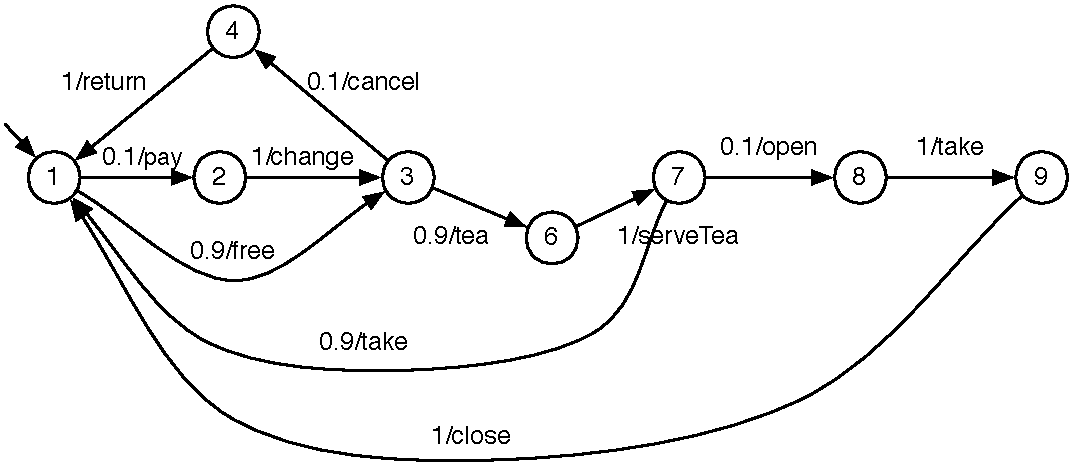
\includegraphics[width=95mm]{svm-usagemodel}
	\caption{Soda vending machine usage model}
	\label{fig:svmusagemodel}
\end{figure}

For instance, Figure \ref{fig:svmusagemodel} presents a usage model of the soda vending machine SPL described in section \ref{sec:casestudy:svm}: each transition has been tagged with a probability which represents, amongst all the possible products of the SPL, the probability of the transition to be fired. As we base our usage model on the actual usage of the product line, some states and transitions may be missing in the usage model if the behaviour linked to those states and transitions has not been observed in any product of the SPL. This corresponds to transitions with a probability equal to 0 and states with only input transitions with a probability equal to 0. In our example, we have no vending machine serving soda. Transitions with actions \textit{soda} and \textit{serve\-Soda} and state 5 have been removed from the usage model presented in Figure \ref{fig:svmusagemodel}.

The usage model is agnostic to the variability inherent to the SPL. It only represents the usage scenarios of the SPL under test as well as their respective probability and serves as basis to select test cases. There are two ways to associate usage scenarios to SPL products:  
%
\begin{itemize}
\item the \emph{family-based} approach \cite{Devroey2014,Devroey2015a} consists in exploiting logs as a source of user information and infer the usage model using machine learning techniques. We can then extract behaviour according to a probability range and relate them to the FTS and feature models of the SPL. As they are extracted from the usage model, behaviours can be run on the FTS to determine which products/features are involved. Some behaviours may also correspond to no product and thus no be executable. Those behaviours are errors coming from the usage model inference or indicators of errors in the FTS. Either case, they can be reported to the test engineer to correct the models.
%
\item the \emph{product-based} approach developed by Samih \etal \cite{Samih2014,Samih2014b} consists in creating usage models from the onset, taking into account requirements and feature models as well as translating expert knowledge to probabilities in the usage model. Concretely, requirements are related to features via a product matrix, while the usage model directly relates its transitions to probabilities and requirements of the SPL. Then, testers have to manually specify the products they are interested in and, with the help of the MaTeLo tool \cite{Samih2014c,matelo}, derive a pruned usage model corresponding  to the behaviour of these products and perform automated test case selection. 
\end{itemize}

%----------------------------------------
\subsection{Product-based test selection}
%----------------------------------------

Product-based test selection is straightforward: the test engineer selects one product to test by selecting features in the feature model, the tool then automatically use the projection operator on FTS to extract a LTS corresponding to the product, and prunes the usage model accordingly. The probabilities of the removed transitions are proportionally distributed on adjacent transitions, so that the probability axiom $\forall s_i \in S : \sum_{s_j \in S, \alpha_k \in \Act} P( s_i , \alpha_k, s_j ) = 1$ holds and balance between the probabilities of the transitions from a same source state are kept \cite{Samih2014b}. Finally, the tool selects test cases using statistical testing algorithms on the usage model~\cite{Whittaker1994,Feliachi2010}.

This scenario is proposed by Samih \etal \cite{Samih2014,Samih2014b} in the MaTeLo Product Line Manager (MPLM) tool \cite{Samih2014c}.  Product selection is made on an orthogonal variability model (OVM) and mapping between the OVM and the usage model (build by a system expert using MaTeLo \cite{matelo}) is provided via explicit traceability links to functional requirements. This process requires to perform the selection of the product of interest on the variability model and does not exploit the usage model during this selection. 


%----------------------------------------
\subsection{Family-based test selection}
%----------------------------------------

Contrary to product-based test selection, family-based test selection supports partial coverage of the SPL by the usage model (like the soda vending machine usage model presented in Figure \ref{fig:svmusagemodel}). 
The key idea is to select abstract test cases (\ie sequences of actions, not necessarily executable by one product of the SPL) from the usage model according to their probability to happen using an interval given by the engineer. Only abstract test cases from the model with a probability in this interval are considered. \Eg one may be interested in analysing highly probable behaviours (interval $[0.5 , 1]$). Only one abstract test case has a probability in this range in the soda vending machine usage model: $Pr(free, tea,serveTea,take) = 0.729$, which corresponds to the behaviour ``serving tea for free''.
The selected abstract test cases are filtered using the FTS in order to keep only positive abstract test cases (executable by at least one product of the SPL) and a pruned FTS (FTS'). The FTS' represents the minimal behaviour of the FTS needed to execute the positive abstract test cases, it is used latter to prioritize the products to test (see section \ref{sec:coverage:usage:prioritisation}).

\paragraph{Abstract test case selection from the usage model:}
%------------------------------------------------------------

The first step is to extract abstract test cases from the usage model according to the desired parameters. 
To perform abstract test case selection in a usage model $dtmc$, we apply an all-paths algorithm parametrized with a maximum length $l_{max}$ for finite abstract test cases and an interval $[Pr_{min} , Pr_{max}]$ specifying the minimal and maximal values for the probabilities of selected abstract test cases. 
Formally: 
\begin{align*}
    allpaths & (l_{max} , Pr_{min}, Pr_{max}, dtmc) =
        \{(i,\alpha_1 , ... , \alpha_{n}, i) \mid \\ 
        & n < lmax \wedge ( \nexists k : 0 < k < n, i = s_k ) \\
 \wedge &  (Pr_{min} \leq Pr(i,\alpha_1 , ... , \alpha_{n}, i) \leq Pr_{max})\}
\end{align*}
where 
$$Pr(i, \alpha_0, \dots, s_n) =\prod_{j=0}^{n-1} P_{dtmc}(s_j, \alpha_j , s_{j+1}).$$

We initially consider only (finite) abstract test cases starting from and ending in the initial state~$i$ (assimilated to an accepting state) without passing by~$i$ in between.  These abstract test cases correspond to a coherent execution scenario in the usage model. The $l_{max}$ bound allows the algorithm to scale to large usage models \cite{Devroey2014}.

The interval $[Pr_{min} , Pr_{max}]$ is provided by the engineer based on his knowledge of the SPL and the selection purpose: an interval with high values (\eg $[0.5 , 1]$) gives highly probable behaviours of the SPL. This is often desired for a non-regression testing scenario where the engineer wants to ensure that the main functionalities of a SPL are still  reliable after an update \cite{Mathur2008}. 
The engineer may also be interested in testing behaviours with a low probability as they may find rare bugs not discovered by the users of the products. Such strategies can be used, \eg for intrusion detection \cite{GarciaTeodoro2009}. 

The interval, its relevance, and selected test cases depend on the usage model source (\eg built from running products, manually built by an engineer, \etc) and the usage model shape (\ie number of states, transitions, average states degree, \etc). To have an idea of the interval to choose and the number of abstract test cases that are selected, the engineer may use random walks in the usage model to select random abstract test cases with their probability and see how they are distributed.

Practically, this algorithm builds an exploration tree where each node represents the exploration of a state. The exploration of a branch of the tree is stopped when the depth is higher than~$l_{max}$. This parameter is provided to the algorithm by the test engineer and is used to avoid infinite loops during the exploration of the usage model. 

For instance, the execution of the algorithm on the soda vending machine example ($um_{svm}$) presented in Figure \ref{fig:svmusagemodel}, with a $l_{max}$ value of 7 (the size of the maximal simple path) and an interval $[0, 0.1]$ to capture the least probable abstract test cases, gives 5 finite abstract test cases: 
\begin{align*}
& allpaths  (7 ;  0 ; 0.1 ; um_{svm}) = \{ \\ 
    & (pay, change, cancel, return) ; (free, cancel, return) ;\\
    & (pay, change, tea, serveTea, open, take,  close); \\
    & (pay, change, tea, serveTea, take) ; \\
    & (free, tea, serveTea, open, take, close)
    \}
\end{align*}
During the execution of the algorithm, the abstract test case \textit{(free, tea, serve\-Tea, take)} has been rejected since its probability ($0.729$) is not between $0$ and $0.1$.

The downside is that the algorithm may possibly enumerate all the paths in the usage model depending on the~$l_{max}$ value. This can be problematic and we plan in our future work to use symbolic executions techniques inspired by work in the probabilistic model checking area, especially automata-based representations \cite{Classen2011} in order to avoid exploring all paths.


\paragraph{FTS-based abstract test case filtering and FTS pruning:}
%-----------------------------------------------------------------

\begin{algorithm}[t]
	\KwIn{$\fts=(S,Act,\mathit{trans},i,d,\gamma)$: a connected FTS;\\
		  $s$: the set of abstract test cases to filter}
	\KwOut{$\fts'$, an FTS representing $\fts$ restricted to the behaviour in $s$, and $s'$, the set of positive abstract test cases from $s$}
	\Begin{
		$S' = \{i\}$; $\Act' = \emptyset$; $\trans'= \emptyset$; $i' = i$; $d' = d$; $\gamma' = \emptyset$\; \nllabel{algo:abstracttestcasesfiltering:line:init}
		$s' = s$\; \nllabel{algo:abstracttestcasesfiltering:line:init2}
		\For{$t \in \wTraces$ \nllabel{algo:abstracttestcasesfiltering:line:foreachtestcase}}{
			\eIf{$\exists s_k \in S,\: \fts \overset{t}{\Longrightarrow}s_k$ \nllabel{algo:abstracttestcasesfiltering:line:ifexecutable}}{
				$\Act' = \Act' \cup t$\; \nllabel{algo:abstracttestcasesfiltering:line:addaction}
				$S' = S' \cup \wStates(\fts, t)$\; \nllabel{algo:abstracttestcasesfiltering:line:addstates}
				$\trans' = \trans' \cup \wTransitions(\fts, t)$\; \nllabel{algo:abstracttestcasesfiltering:line:addtransitions}
				$\gamma' = \wFLabels(\fts, t) \gamma'$\; \nllabel{algo:abstracttestcasesfiltering:line:addfexpr}
			}{
				$s' = s' \setminus \{t\}$\; \nllabel{algo:abstracttestcasesfiltering:line:removetestcase}
			}
		}
		$\fts' = (S', \Act', \trans', i', d', \gamma')$\;
  		\Return $(\fts', s')$\; \nllabel{algo:abstracttestcasesfiltering:line:return}
	}
	\caption{FTS' building and positive abstract test cases filtering}
 \label{algo:abstracttestcasesfiltering}
\end{algorithm}

We do not make any assumptions about the source of the usage model. Therefore, this step serves as a sanity check to ensure that selected traces correspond to behaviour that may be executed by at least one valid product of the SPL. If this is not the case, there is an error in the usage model or in the FTS. 
Depending on how the model has been built, the error may come from the engineer (\eg missing transition/state, extra transition/state, wrong feature expression on a transition of the FTS, \etc during the modelling) or from the model inference method used to generate the model from a set of execution traces. Such errors have to be detected and reported to the engineer who has to decide what to do: either correct the usage model or the FTS in order to avoid illegal behaviours; or ignore the error if it is not significant.
 
The idea to filter abstract test cases and keep only positive abstract test cases is to use the FTS to detect negative abstract test cases by running them on it.
%
Practically, we build a second \emph{FTS} which represents only the behaviour of the SPL appearing in the positive abstract test cases selected from the usage model. This FTS' represents a prioritized subset of the original FTS \cite{Devroey2014e}.

Algorithm \ref{algo:abstracttestcasesfiltering} presents how to build the FTS' ($\fts'$) from a set of abstract test cases ($s$), with positive abstract test cases filtered during the algorithm (into $s'$), and a given FTS ($\fts$). 
The initial state of $fts'$ corresponds to the initial state of the $\fts$ (line \ref{algo:abstracttestcasesfiltering:line:init}) and $d$ in $\fts'$ is the same as for $\fts$ (line \ref{algo:abstracttestcasesfiltering:line:init}). 
For each abstract test case, if it is executable on $\fts$ (line \ref{algo:abstracttestcasesfiltering:line:ifexecutable}), then the states ($states(fts, t)$), actions ($t$) and transitions ($\wTransitions(fts, t)$) visited in $\fts$ when executing the trace $t$ are added to $\fts'$ (line \ref{algo:abstracttestcasesfiltering:line:addaction} to \ref{algo:abstracttestcasesfiltering:line:addtransitions}). 
%
On line~\ref{algo:abstracttestcasesfiltering:line:addfexpr}, the $\wFLabels(\fts, t)$ function is used to enrich the $\gamma'$ function with the feature expressions of the transitions visited when executing $t$ on the $\fts$. It has the following signature: 
%
$$\wFLabels : (\FTS, \Act^{*}) \rightarrow (\trans \mapsto \Sem{d} \mapsto \mathbb{B}) \rightarrow (\trans \mapsto \Sem{d} \mapsto \mathbb{B})$$
%
On line \ref{algo:abstracttestcasesfiltering:line:addfexpr}, $\wFLabels (\fts, t) \gamma_{\fts'}$ returns a new function $\gamma'_{\fts'}$ which, for a given transition $tr = (s_i \overset{\alpha_k}{\longrightarrow}  s_{j}) $, returns $\gamma_{\fts} (tr)$ if $\alpha_k \in t$ or $\gamma_{\fts'} (tr)$ otherwise.

\begin{figure}
	\centering
	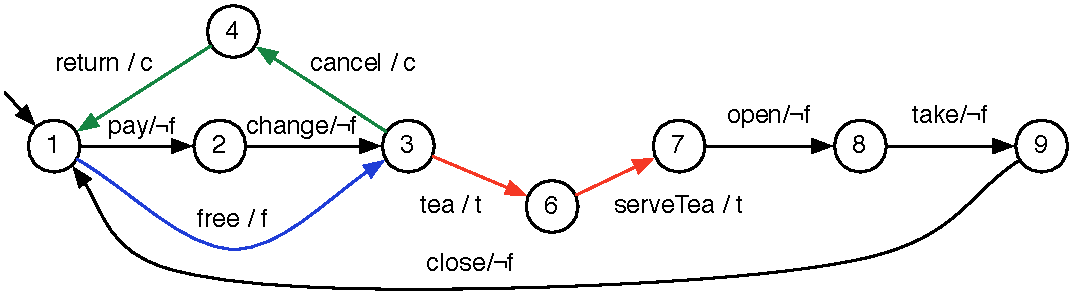
\includegraphics[width=95mm]{svm-ftsprime}
	\caption{Soda vending machine FTS'}
	\label{fig:svmftsprime}
\end{figure}

In our example, the set of finite traces with a probability between 0 and 0.1 selected in step~1 contains two negative abstract test cases: \textit{(pay, change, tea, serve\-Tea, take)} and \textit{(free, tea, serve\-Tea, open, take, close)}, which both lead to an execution condition containing the $free \wedge \neg free$ feature expression. Those 2 negative abstract test cases (mixing free and not free vending machines) cannot be executed on the soda vending machine  FTS (of Figure \ref{fig:svmfts}) and are rejected by Algorithm \ref{algo:abstracttestcasesfiltering}. The generated FTS' is presented in Figure \ref{fig:svmftsprime}.

%-----------------------------------
\subsection{Product prioritisation}
%-----------------------------------

\label{sec:coverage:usage:prioritisation}

Product-based test selection assumes that relevant products from which test cases are selected have already been prioritized. Relevant products are used to prune the usage model (in order to keep only the behaviour of the selected product) and test cases are derived using a statistical testing algorithm.

When performing a family-based test selection from a usage model, relevant abstract test cases are directly selected from the usage model representing the behaviour of the SPL. Those abstract test cases are then filtered to keep only positive abstract test cases. At the end of algorithm \ref{algo:abstracttestcasesfiltering}, we have an FTS' and a set of (positive abstract) test cases. This set of test cases covers all states and transitions of the FTS'. Since they come from the usage model, it is possible to order them according to their probability to happen. This probability corresponds to the the cumulated individual probabilities of the transitions fired when executing the finite trace in the usage model. 
A test case $t=(i, \alpha_1 , \ldots , \alpha_n, i)$ corresponding to a path $(i \overset{\alpha_1}{\longrightarrow} \ldots \overset{\alpha_n}{\longrightarrow} i)$ in the usage model has a probability $\wPr(i, \alpha_1 , \ldots , \alpha_n, i)$ to be executed. 

At this step, each test case $t$ is associated to the set of products $\wProd(t,\fts')$ that can actually execute~$t$. Product prioritisation may be done by sorting the test cases according to their probability to be executed, giving a set of products for each test case $t$.

For instance, for the positive abstract test case $t = $ \textit{(pay, change, tea, serve\-Tea, open, take, close)}, selected for our example, the products have to satisfy: $$\neg f \wedge t \wedge \CNF(d)$$
Where $d$ is the feature model of the soda vending machine (presented in Figure \ref{fig:svmfm}), transformed into a boolean formula using the $\CNF$ function.
This gives us a set of 8 products (amongst 32 possible):
\begin{align*}
\{&(v, b, cur, t, eur) ; (v, b, cur, t, usd) ; (v, b, cur, t, c, eur) ; \\
& (v, b, cur, t, c, usd) ; (v, b, cur, t, s, eur) ; (v, b, cur, t, s, usd) ;\\
&(v, b, cur, t, s, c, eur) ; (v, b, cur, t, s, c, usd) \}
\end{align*}
Each of them executing $t$, which is the behaviour of the soda vending machine product line with the lowest probability ($\wPr(t) = 0.009$ in the usage model). 

%-------------------------
\subsection{Related work}
%-------------------------

To the best of our knowledge, there is no approach prioritizing behaviours statistically for testing SPLs in a family-based manner.  
There have been SPL test efforts to sample products for testing such as t-wise approaches \cite{Perrouin2011,Cohen2006,Cohen2008,Johansen2012}. More recently sampling was combined with prioritisation thanks to the addition of weights on feature models and the definition of multiple objectives \cite{Johansen2012b,Henard2014a}. However, these approaches do not consider SPL behaviour in their analyses.  

Efforts to combine sampling techniques with modelling ones (\eg \cite{Lochau2011}) exist.  These approaches are product-based, meaning that they may miss opportunities to reuse tests amongst sampled products \cite{VonRhein2013}. We believe that benefiting from the recent advances in behavioural modelling provided by the model checking community \cite{Asirelli2011,Asirelli2011a,Classen2011,Classen2013b,Fischbein2006,Lauenroth2009,Rodrigues2015,terBeek2016}, sound MBT approaches for SPL can be derived and interesting scenarios combining verification and testing can be devised.

To consider behaviour in an abstract way, a full-fledged MBT approach \cite{Utting2007} is required. Although behavioural MBT is well established for single-system testing~\cite{Tretmans2008}, a survey  \cite{Oster2011} shows insufficient support for SPL-based MBT. Metzger and Pohl further emphasizes the need for inter-model consistency  and minimizing test redundancy  across the lifecycle (domain and application engineering) \cite{Metzger2014}. We believe that the FTS formalism, natively equipped with features as a first-class concept, is pivotal  to inter-model verification support and supports combination of quality assurance techniques both at the domain and application engineering levels as our integration between family-based and product-based statistical test selection illustrates.  

Our will is to apply ideas stemming from statistical testing \cite{Sprenkle2013} and adapt them in an SPL context. For example, combining structural criteria with statistical testing has been discussed by Gouraud \etal  \cite{Gouraud2001} and Th\'evenod-Fosse and Waeselynck \cite{Thevenod-Fosse1991}. We do not make any assumption on the way the usage model is obtained: via an operational profile \cite{Musa1996}, by analysing the source code or the specification \cite{Thevenod-Fosse1991}, or from the running application logs \cite{Ghezzi2014,Sprenkle2013}. In the absence of a source of information for the usage model, one could think of a uniform distribution of probabilities over the usage model. As noted by Whittaker \cite{Whittaker1994}, in such case, only the structure of abstract test cases would be considered and therefore basing their selection on their probabilities would just be a means to limit their number in a mainly random testing approach. In such cases, it is better to use structural test selection  \cite{Feliachi2010}.

We use MaTeLo \cite{matelo} to select test cases from a product model. Other tools like JUMBL \cite{Prowell2003} would have qualified. Both are model-based statistical testing tools, supporting the development of statistical usage models using Markov chains, the analysis of models, and the selection of test cases \cite{Utting2012}. However, none of them are able to natively handle SPL models. We use the MaTeLo Product Line Manager (MPLM) tool \cite{Samih2014,Samih2014b} to generate models for a product of the SPL, which are then used to select test cases. 


%%%%%%%%%%%%%%%%%%%%%%%%%%%%%%%%%%%%
\section{Wrap up}
%%%%%%%%%%%%%%%%%%%%%%%%%%%%%%%%%%%%

In this chapter, we described three abstract test case selection and prioritisation approaches: structural, dissimilarity, and usage based test cases selection criteria. 

\paragraph{Structural selection criteria:}
%--------------------------------------------

Structural selection and prioritisation criteria are based on the structure of the \gls{FTS} representing the product line to test. Those criteria consider the number of states, actions, transitions, transitions-pairs, or paths covered in the FTS to guide the abstract test case selection. Once selected, the prioritisation of the products to test is done according to the abstract test cases executable by those products: products that can reach the best coverage by executing as many test cases as possible and/or those with the best coverage are ranked first. 

\paragraph{Dissimilarity selection criteria:}
%--------------------------------------------

Dissimilarity selection criteria aim at selecting abstract test cases as diverse as possible. The dissimilarity is defined by the test engineer by combining basic distance functions taking the actions and products covered by the test cases as input. We used a (1+1) without mutation nor crossover evolutionary algorithm to select the test cases, based on a given time budget and a given size of the test suite.

\paragraph{Usage selection criteria:}
%--------------------------------------------

Usage-based selection criteria may be used in two ways: family-based and product-based test selection and prioritisation. Family-based selection and prioritisation extracts products of interest according to the probability of their execution traces gathered in a usage model.  We thus select a subset of the full SPL behaviour given as a \gls{FTS}. This allows us to construct a new FTS, FTS', representing only the executions of relevant products.  This FTS' can be analysed all at once to enable test reuse amongst products to scale during testing activities. Product-based selection and prioritisation requires the testers to select a product of interest before the usage model is pruned, leaving only its executions associated to it \cite{Samih2014b,Samih2014,Samih2014c}. Though these approaches may seem antagonistic, family-based prioritisation can gracefully complement the product-based one by suggesting products of interest.


\chapter{Mutation analysis}
\label{chap:mutation}

Mutation analysis is an established technique to either evaluate test suite effectiveness \cite{Andrews2006,Offutt2011,Gligoric2013} or support test case selection \cite{Papadakis2010,Fraser2014,Offutt2011}. It works by injecting artificial defects, called \emph{mutations}, into the code or the model under test, yielding \emph{mutants}, and measures test effectiveness based on the number of detected mutants.

Researchers have provided evidence that detecting mutants results in finding real faults \cite{Andrews2006,Just2014} and that test cases designed to detect mutants reveal more faults than other test case selection criteria \cite{Offutt2011,Baker2013}. This has been shown to be the case for model-based mutation too \cite{Belli2016}: Aichernig \etal \cite{Aichernig2014a} report that model mutants lead to test cases that are able to reveal  implementation faults that were neither found by manually defined test cases, nor by the actual operation, of an industrial system. In addition, model-based mutation's premise is to identify defects related to missing functionality and misinterpreted specifications \cite{Budd1985}. This is desirable since code-based testing fails to identify these kinds of defects \cite{Howden1976,Voas1997}. 

Despite its advantages and the advances made by the research community, mutation analysis still faces important issues \cite{Jia2011a}:
\begin{enumerate}
\item due to the large number of mutants that needs to be generated and \emph{executed} by the test cases, mutation analysis may be expensive. While this problem has been investigated for code-based mutation \cite{Just2014a,Papadakis2011}, it remains open in the model-based context. Since typical real-word models involve thousands of mutants and test suites involve thousands of test cases, millions of executions are needed. Addressing this problem is therefore vital for the scalability of mutation analysis \cite{Jia2011a,Offutt2011};
%
\item in order to generate mutants that denote subtle faults, Jia and Harman \cite{Jia2008} propose to use \emph{higher order} mutants. A higher order mutant is the results of a mutated mutant, \ie a 2nd-order mutant is generated by applying a mutation to a 1st-order mutant, a 3th-order mutant is generated from a 2nd-order mutant, \etc Empirical evidences show that higher order mutants may be used to subsume first order mutants, reducing the number of mutants to execute \cite{Polo2009}, and are harder to kill, which may be useful to select better test cases \cite{Langdon2010}. As for mutants execution, higher order mutation remains an open challenge in model-based context; 
%
\item the \emph{equivalent mutants problem} concerns the mutants whose behaviour is identical to the original artefact (code or model). As they cannot be distinguished by any test case, those mutants skew the analysis and cannot be used to select new test cases.
\end{enumerate}

We address those issues for model-based mutation using the software product line framework. Artificial defects are injected using \emph{mutation operators} on the model under test, producing a mutant. A mutant is thus a small variation of the model under test and the set of generated mutants may be grouped to form a \emph{mutants family}. Based on this idea, we use variability aware mechanisms (FTSs and feature models) to represent a mutant family \cite{Devroey2016a,Devroey2014f}. 

Mutation analysis, as performed in this chapter, is done following a \emph{product-based} approach. It assumes that a product has been selected, that the FTS has been projected on this product to get the corresponding \gls{LTS}, and that only the subset of test cases executable on this product have been kept in the test suite. An \gls{FTS} and a \gls{feature model} represent here the mutant family for one product (\ie LTS). Discussion on extensions of this work to perform mutation analysis in a family-based approach (\ie on the FTS and feature model of an SPL) is presented in Section \ref{subsec:splmutationanalysis}, along with other perspectives of this thesis.

In the remainder of this chapter, we present model-based mutation analysis and give an example in Section \ref{sec:MBMA}. Section \ref{sec:FMM} presents the \acrfull{FMM} and address the first ans second issues \cite{Devroey2016a}. Section \ref{sec:EMP} applied automata language equivalence to detect equivalent mutants and compares it with two random simulations approaches \cite{Devroey2017}. Finally, we wrap up and present perspectives for our work. 

%%%%%%%%%%%%%%%%%%%%%%%%%%%%%%%%%%%%%%%%
\section{Model-based mutation analysis}
%%%%%%%%%%%%%%%%%%%%%%%%%%%%%%%%%%%%%%%%

\label{sec:MBMA}

\begin{figure}[t]
	\centering
	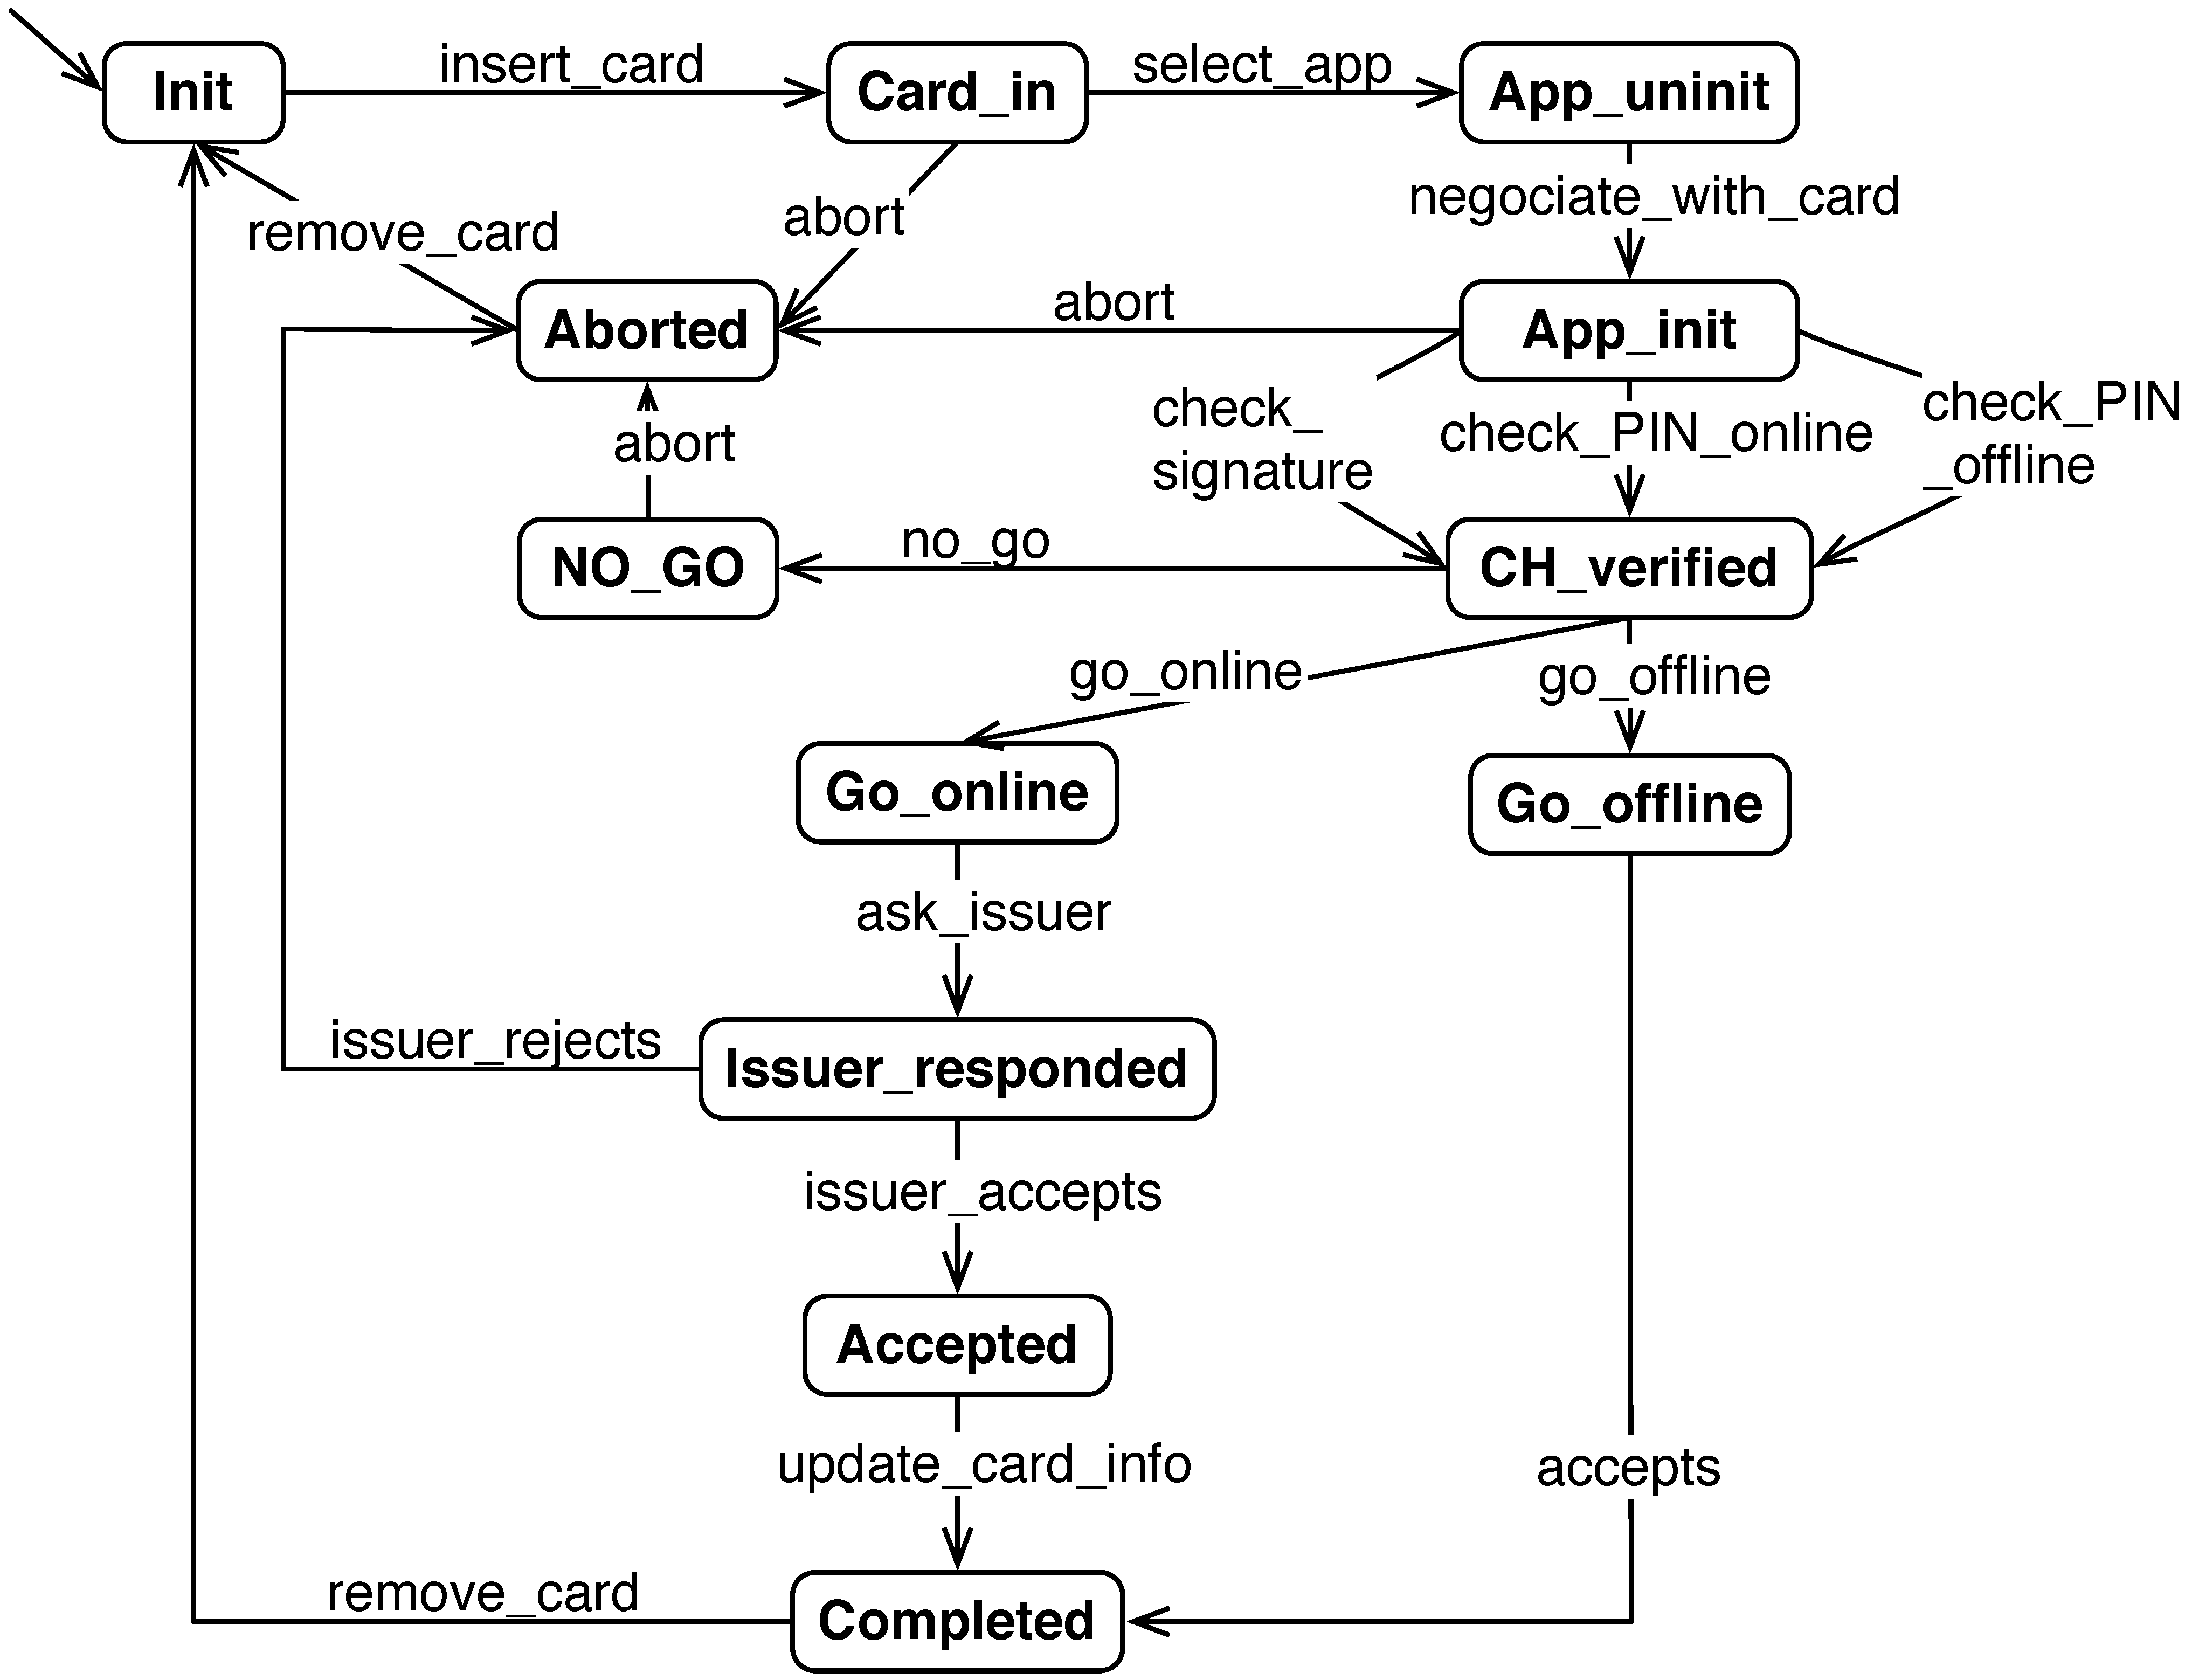
\includegraphics[width=85mm]{card-payment-terminal-product}
	\caption{Card payment terminal product original LTS}
	\label{fig:fmm:cptproduct}
\end{figure}

To address the problems of mutation analysis at the model level, we take our inspiration from our research on software product lines. The idea is to consider mutants as \emph{members} of a \emph{mutants family}\footnote{\textit{Member} is a synonym for \textit{product} or \textit{variant}, and \emph{family} is a synonym for \textit{product line}. For the sake of clarity, we will refer to mutants as \textit{members} of a \textit{mutants family}.}. Considering mutants as part of a family rather than in isolation yields considerable advantages: shared execution at the model level \cite{Classen2013b} and compact representation of a set of mutants. This contrasts with existing product line approaches of mutation analysis \cite{Kim2013a,Nguyen2014,Kim2012a} which require code and hence do not apply to model mutants.

In the following sections, we use as example the specification of one product from the card payment terminal product line described in Section \ref{sec:casestudy:cpterminal}. This product allows both direct debit and credit payments, may perform it online or offline, and allows to identify the card holder using both signature or PIN code. The features from the feature model in Figure \ref{fig:cpterminalfm} selected to form this product are: 
\begin{quote}
$\lbrace$ \textit{CPTerminal, PaymentSchema, DirectDebit, DebitCard, CreditCard, Connectivity, Online, VPN, Offline, CardReader, Chip, MagStrip, Identificator, PIN, Signature} $\rbrace$
\end{quote}
The \gls{LTS} describing the behaviour, obtained using the projection operator on the FTS defined in Figure \ref{fig:cpterminalfts}, is presented in Figure \ref{fig:fmm:cptproduct}.

\begin{figure}[t]
	\centering
	\subbottom[State $\mathit{Go\_offline}$ missing]{
		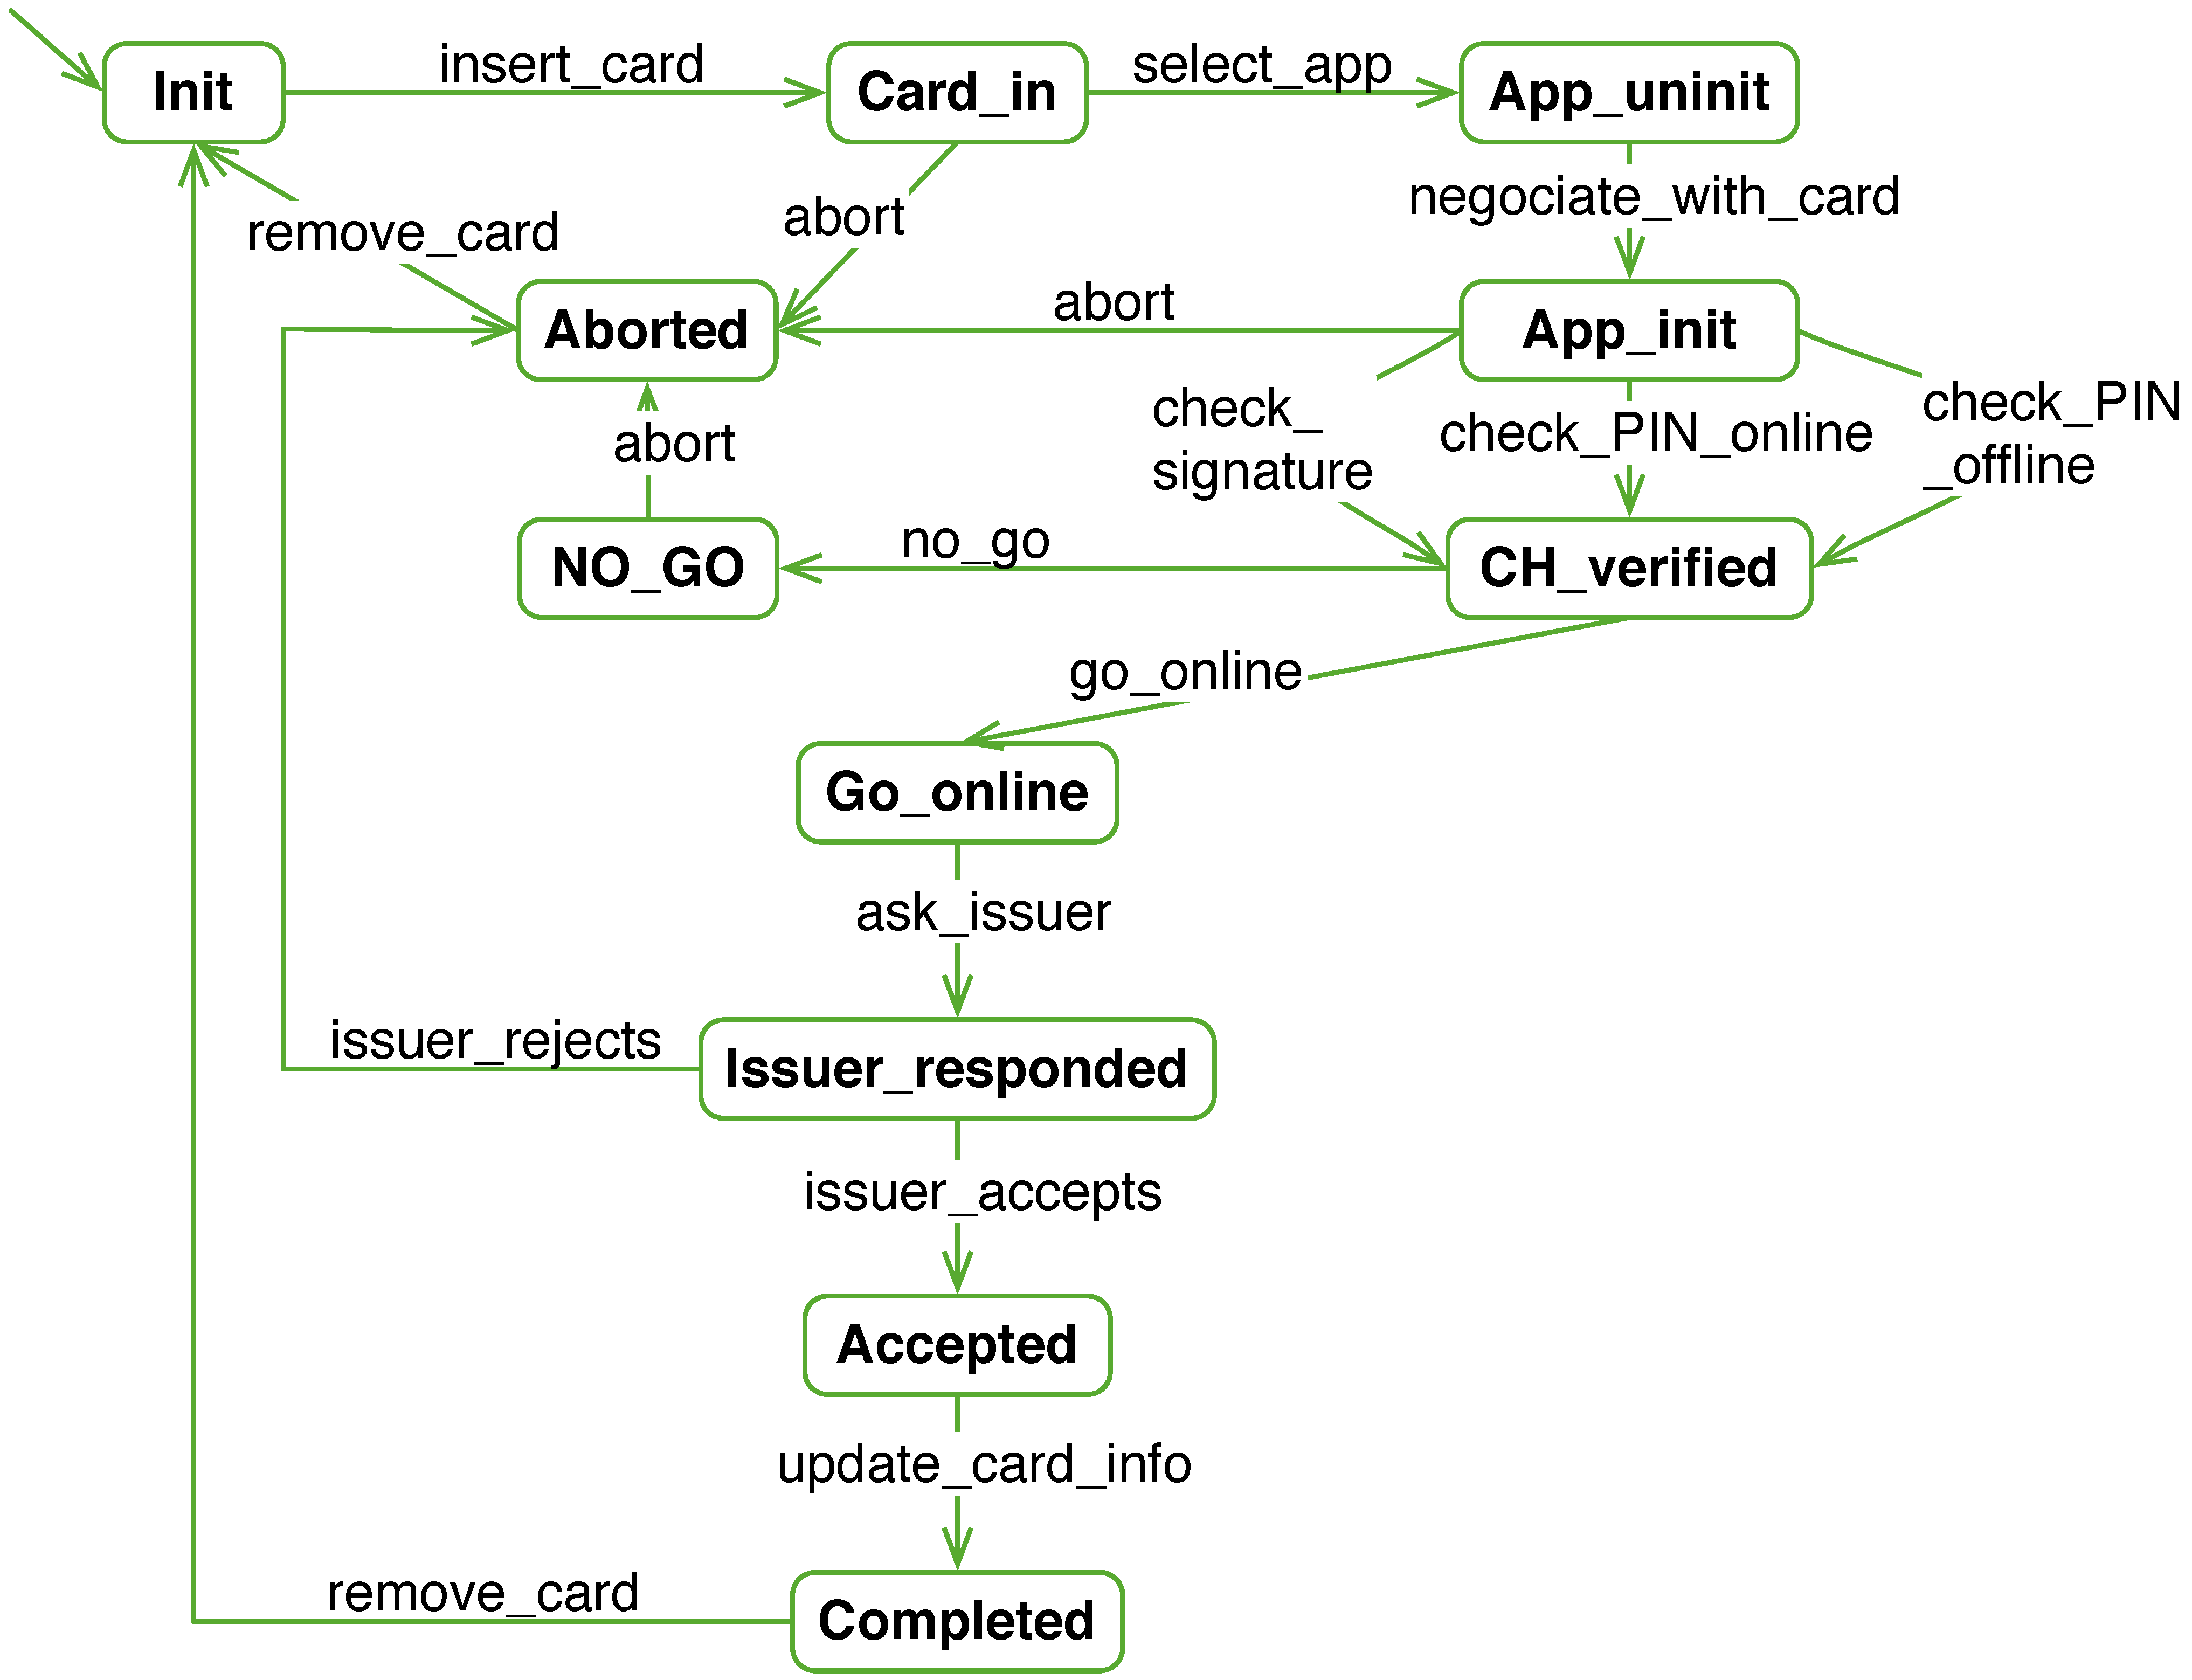
\includegraphics[width=58mm]{cpt-smi_Go_offline}
		\label{fig:fmm:cptsmi}
	}
	\subbottom[State $\mathit{NO\_GO}$ missing]{
		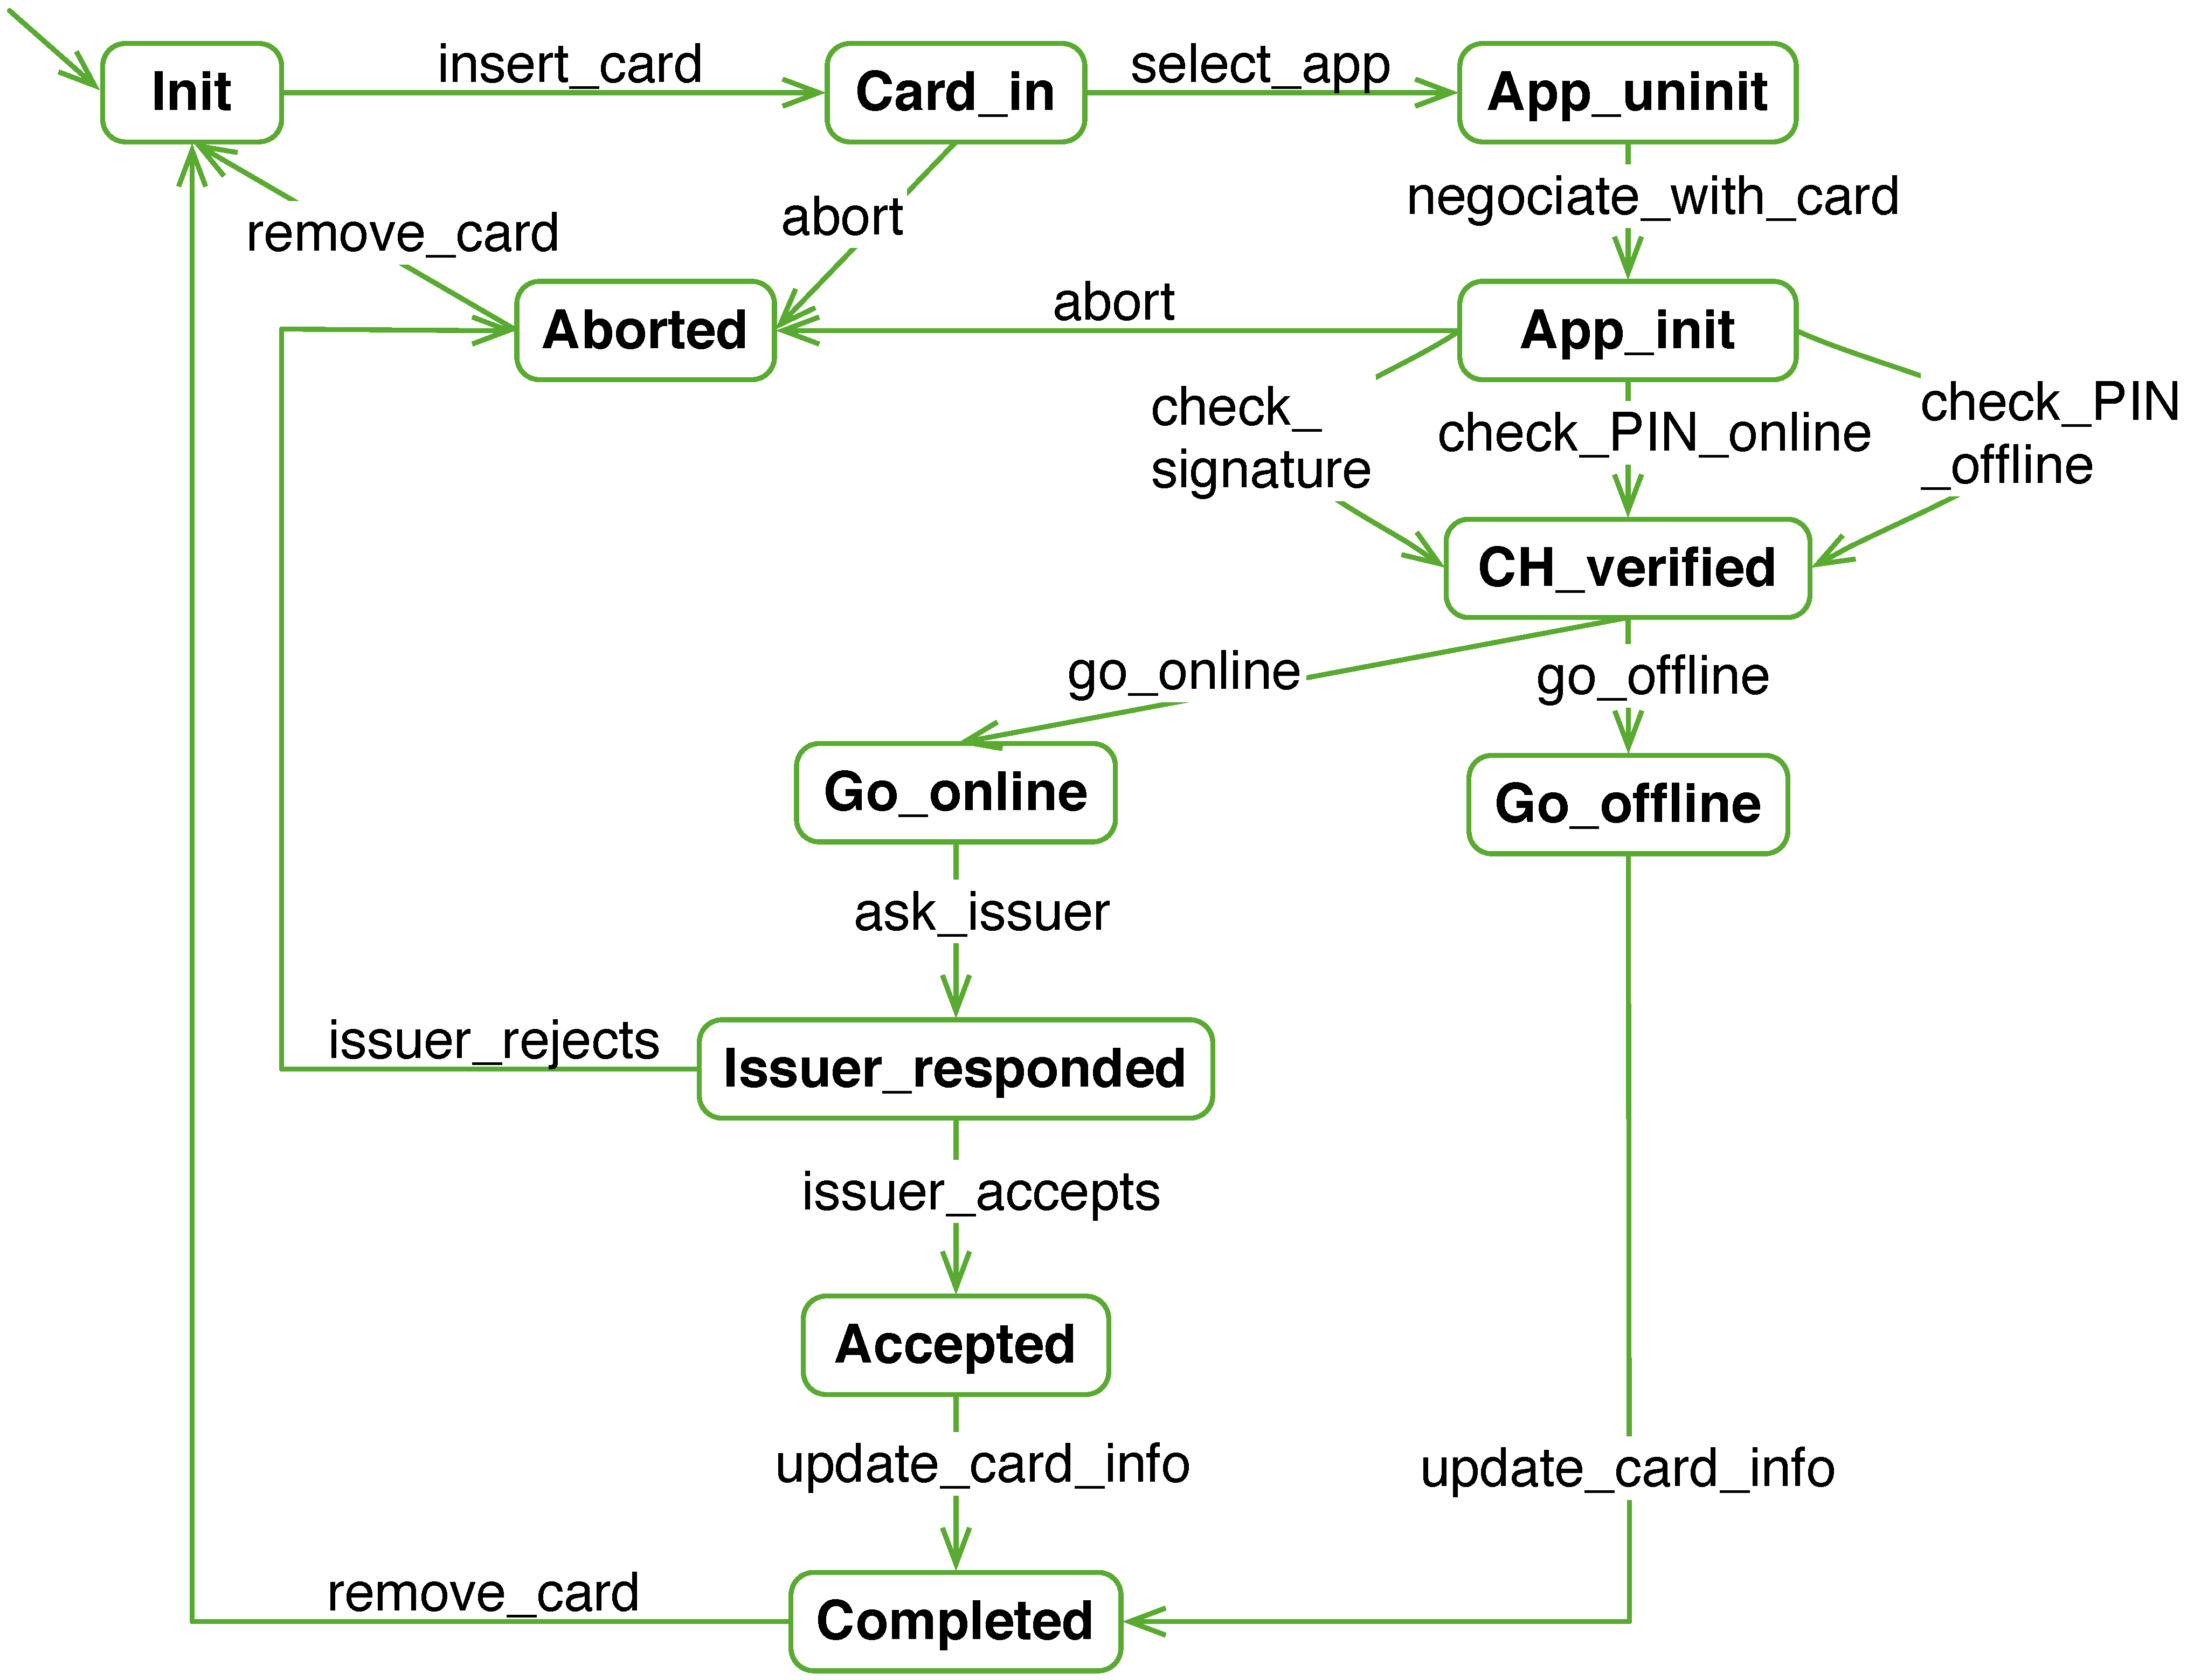
\includegraphics[width=58mm]{cpt-smi_NO_GO}
		\label{fig:fmm:cptsmi2}
	}
	\subbottom[Action $\mathit{issuer\_accepts}$ exchanged]{
		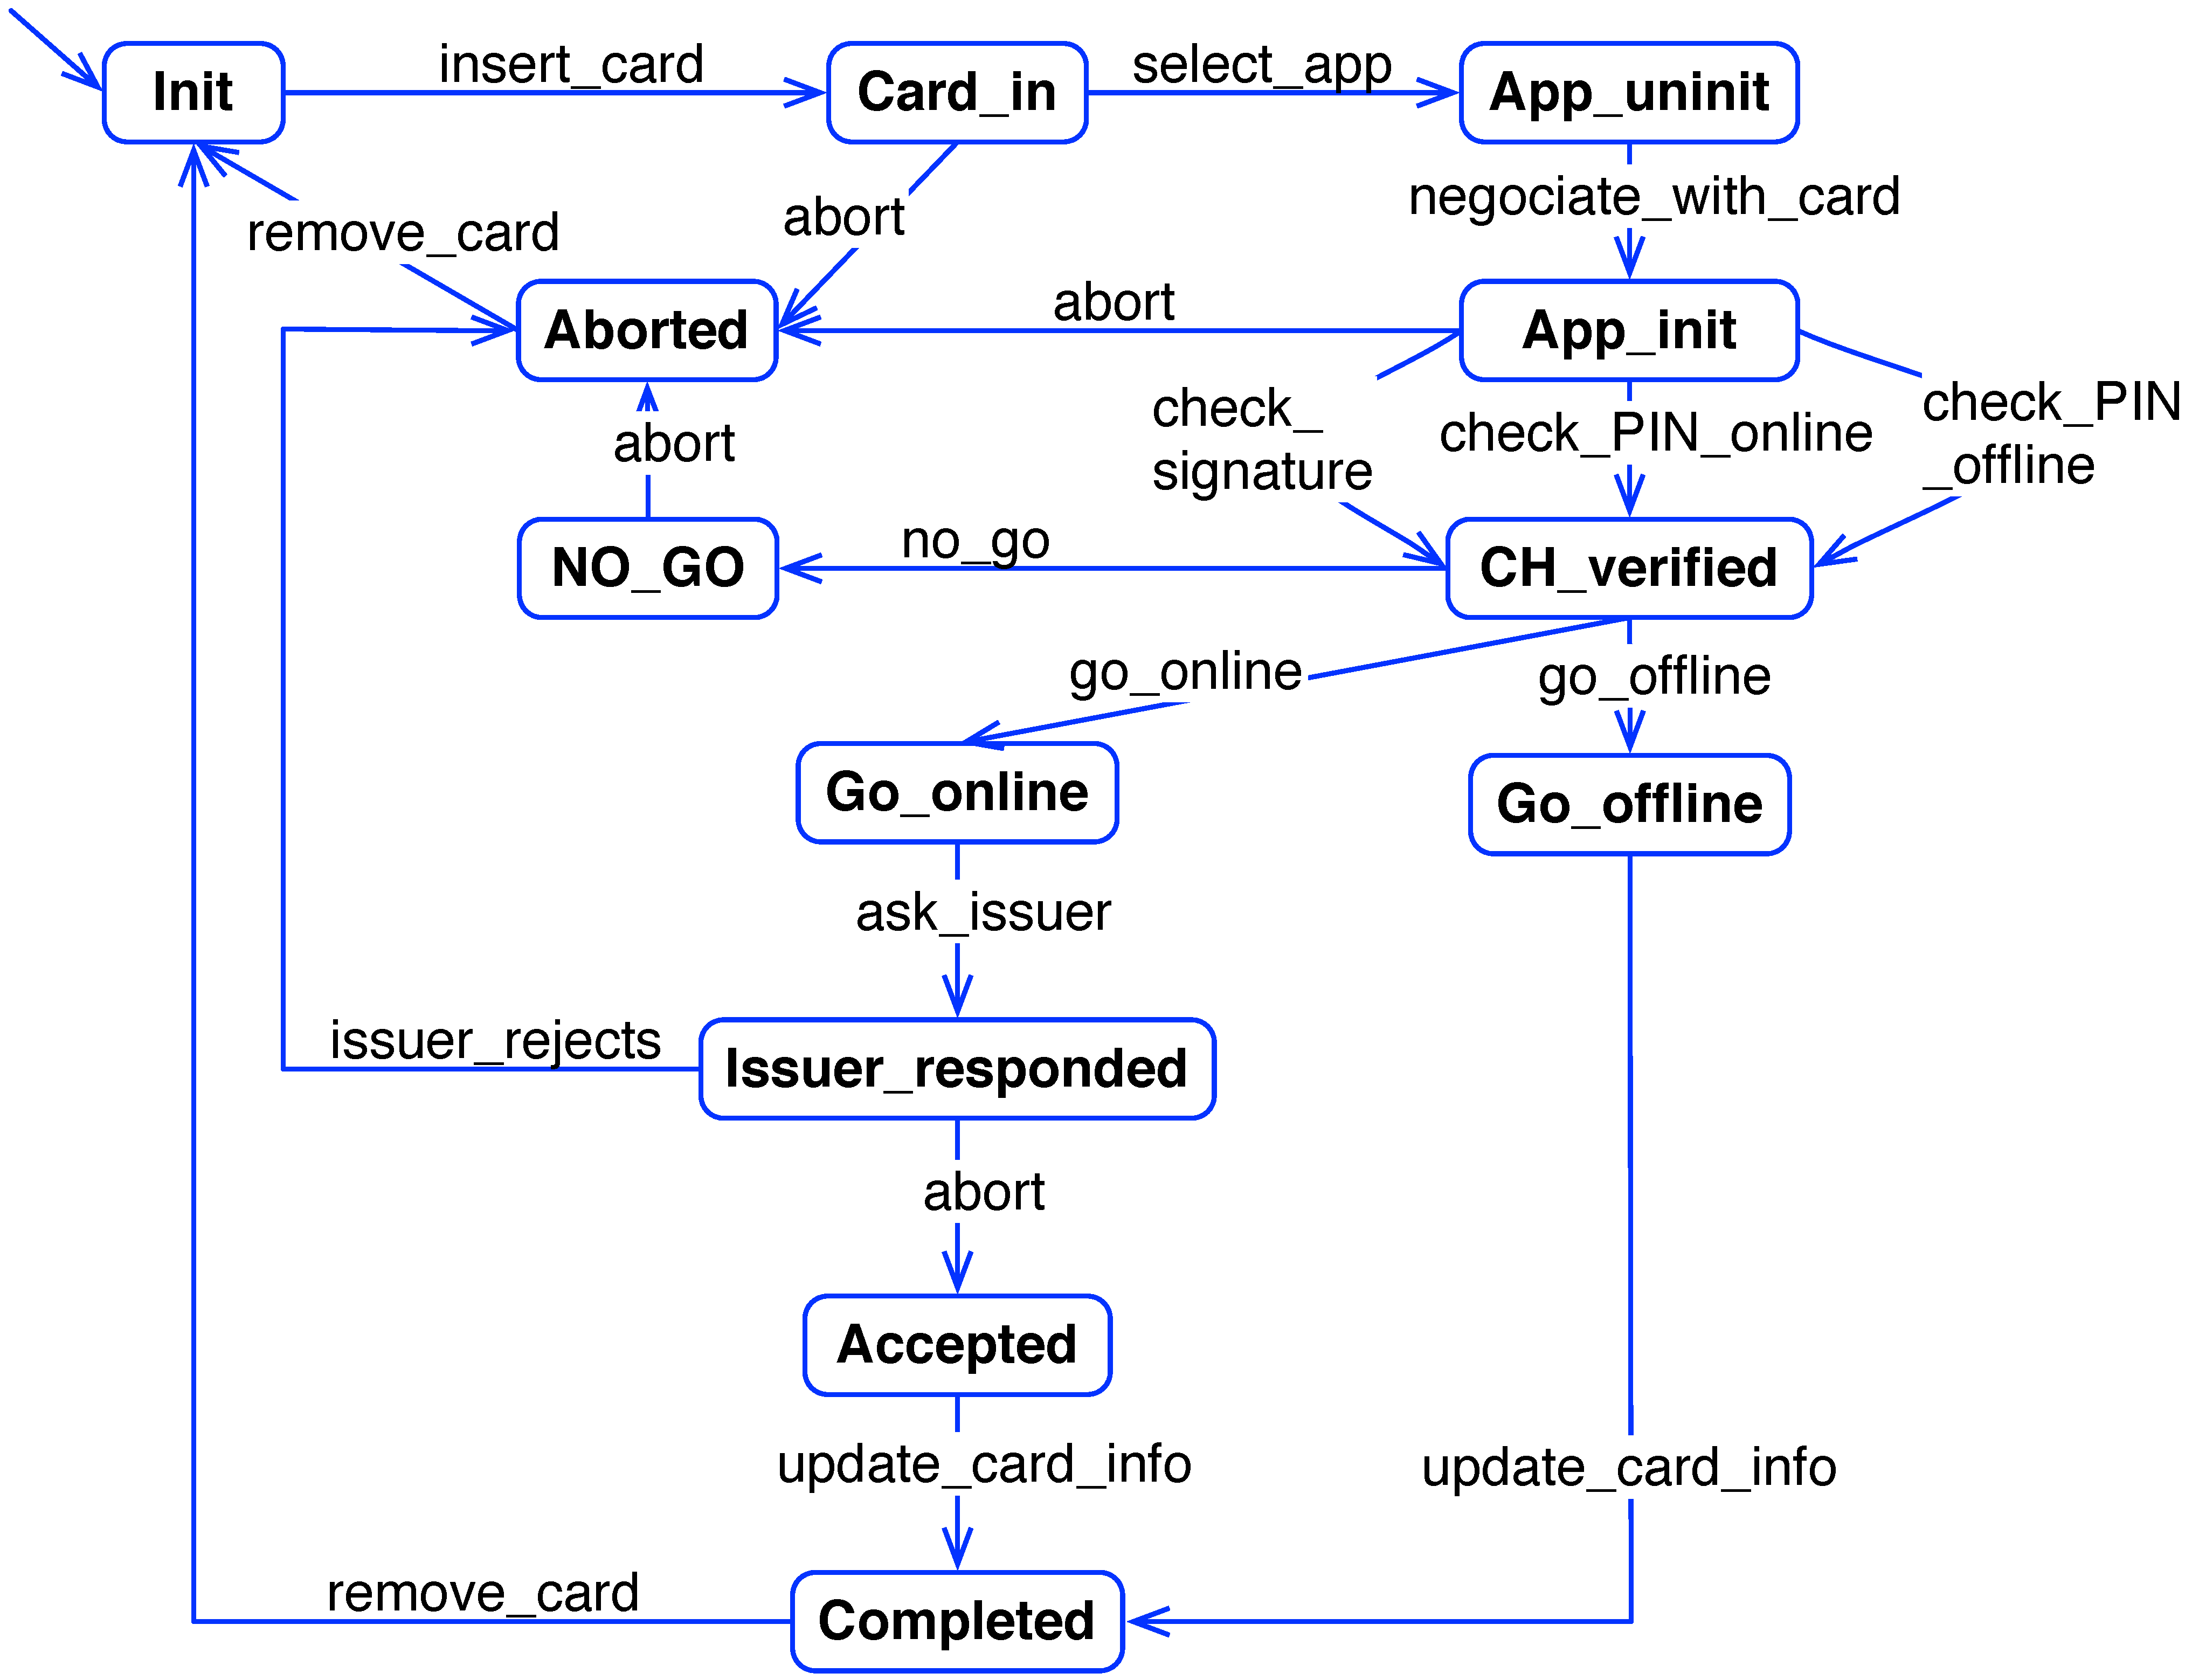
\includegraphics[width=58mm]{cpt-aex_issuer_accepts}
		\label{fig:fmm:cptaex}
	}
	\subbottom[Wrong initial state]{
		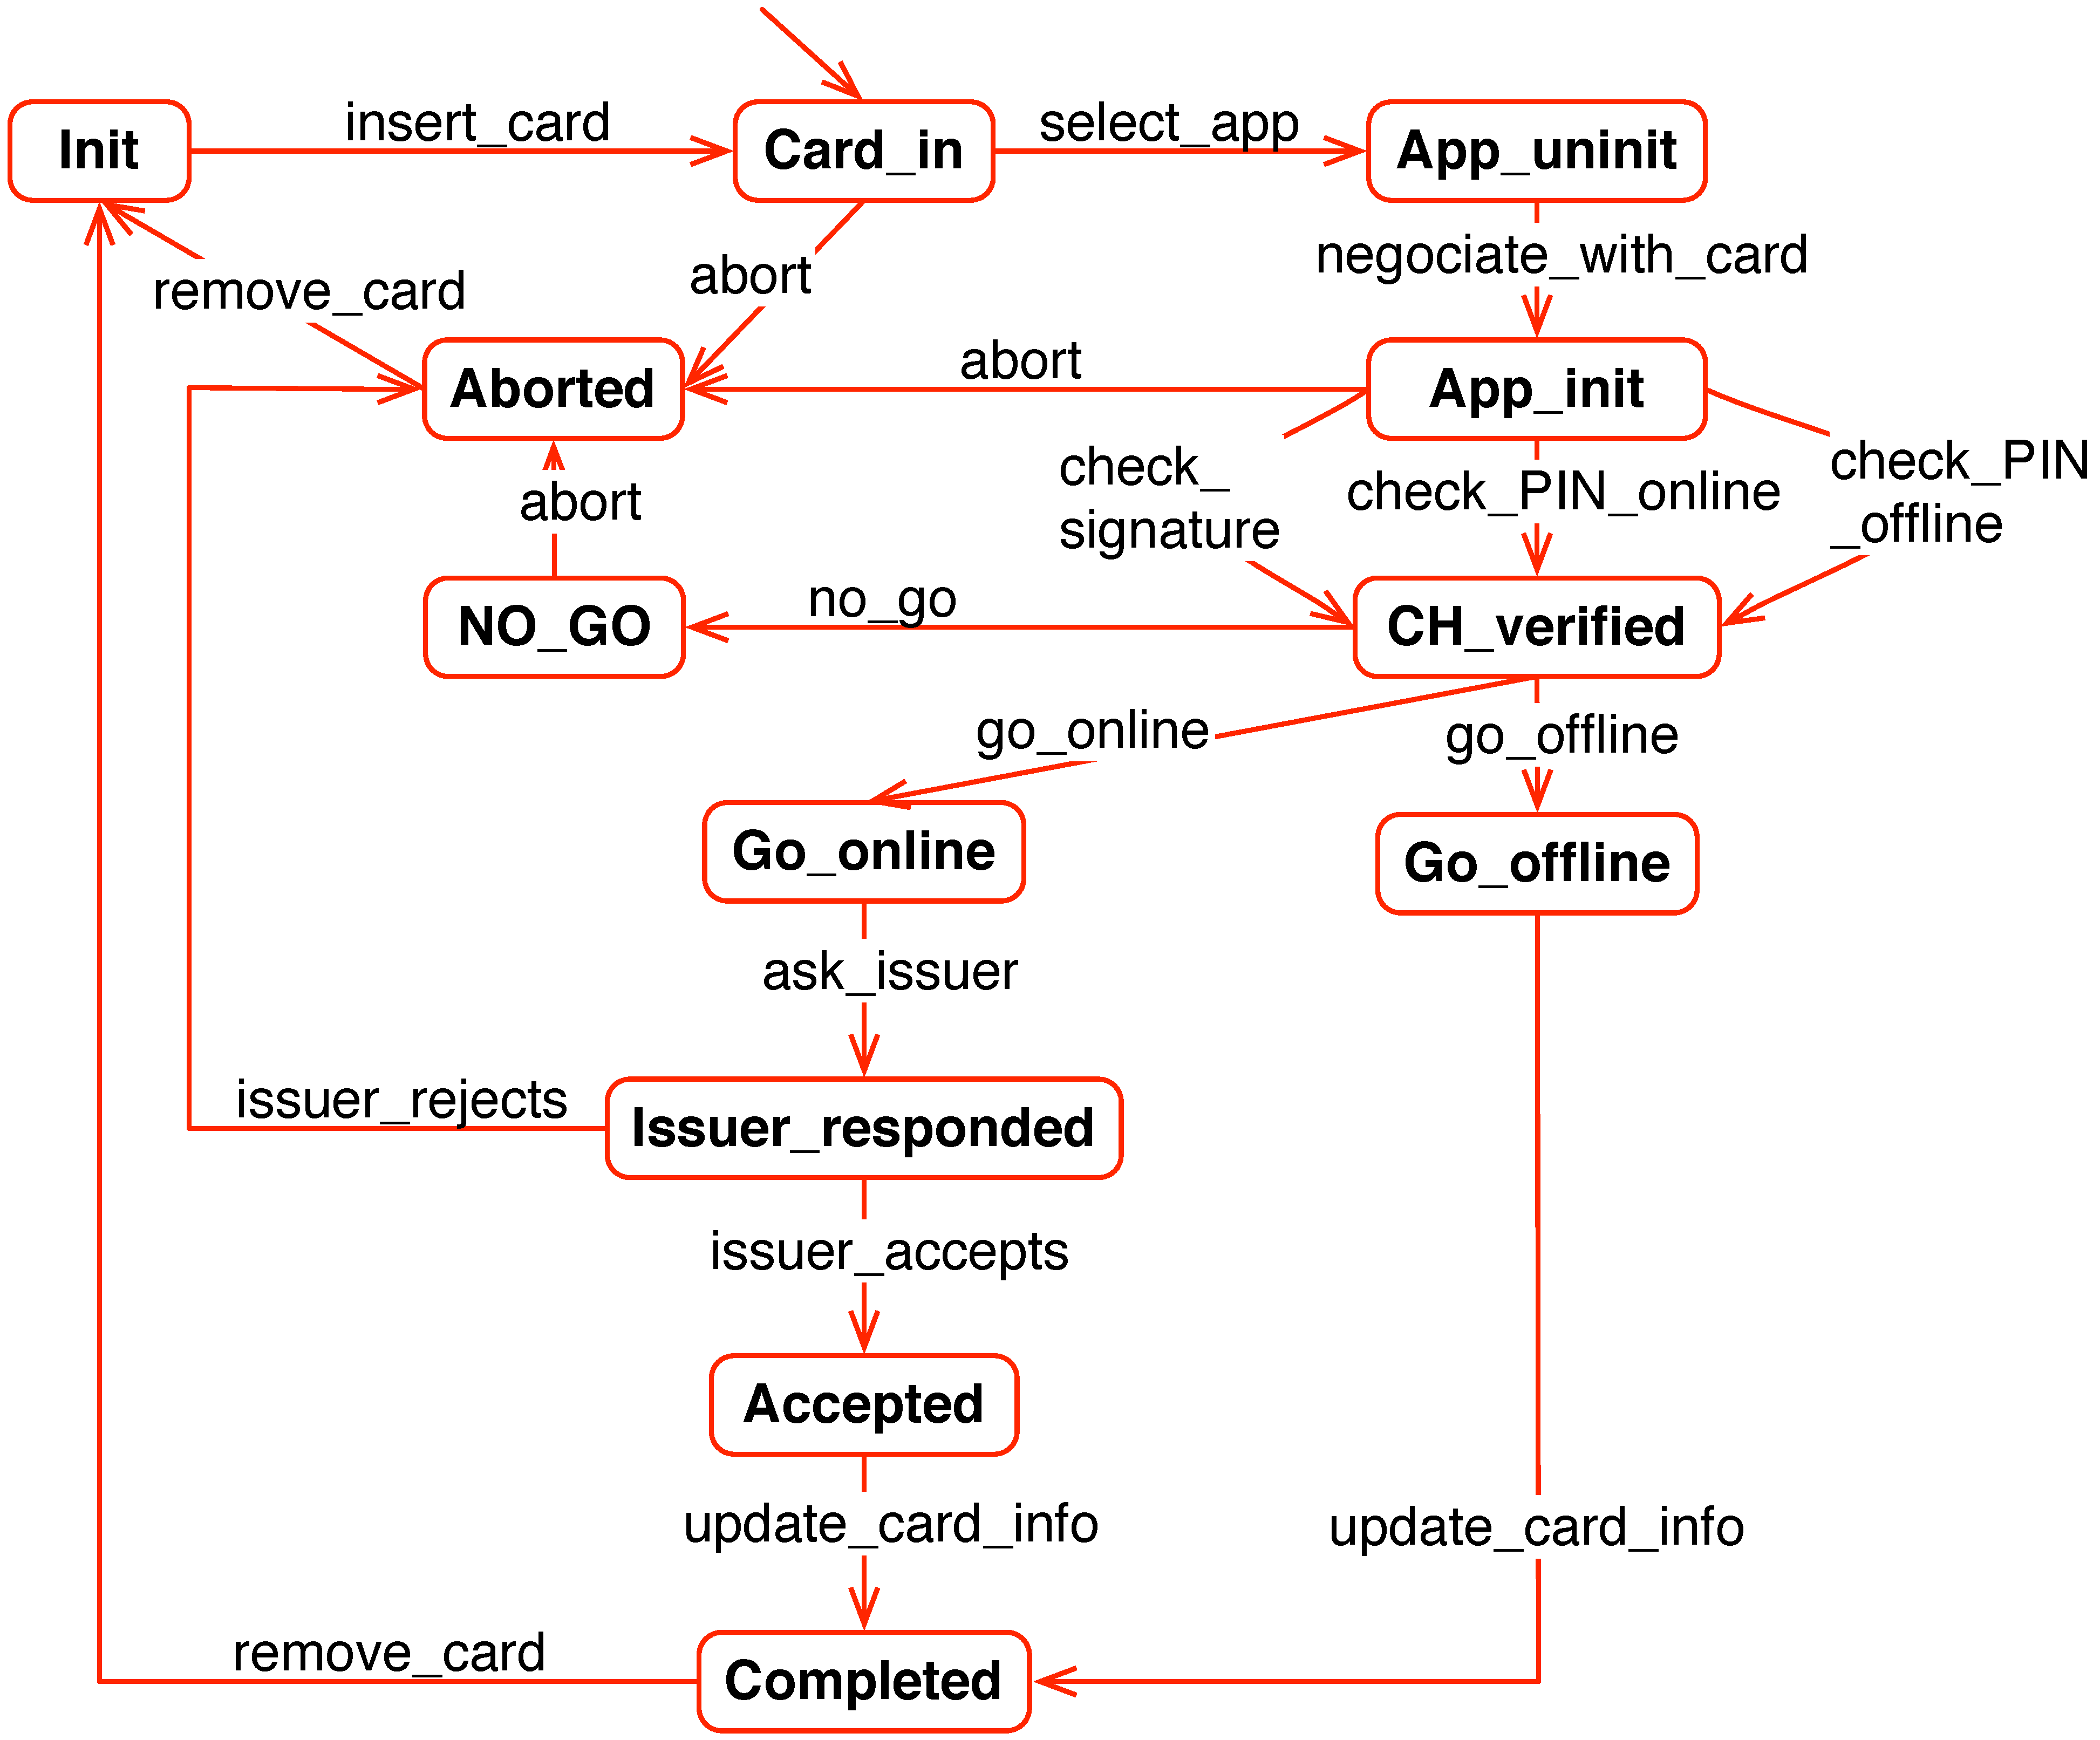
\includegraphics[width=58mm]{cpt-wis_Card_in}
		\label{fig:fmm:cptwis}
	}
	\caption{Card payment terminal product mutants}
	\label{fig:fmm:cptmutants}
\end{figure}

In model-based mutation analysis, mutants are introduced based on model transformation rules, called \emph{mutation operators}, that alter the system specification. Model based mutation is thus a black box testing technique, unlike code-based mutation that requires access to the code and so is white box. An example of mutant obtained from the \textit{state missing operator} applied on the \textit{Go\_offline} state of the card payment terminal system, is presented in Figure \ref{fig:fmm:cptsmi}. There are two kinds of mutants, \textit{first-order} mutants when the original and the mutant models differ by a single model transformation, and \textit{higher order} mutants, derived from the original model after multiple transformations.  

When a mutant is detected by a test case, it is called \emph{killed}. In the opposite situation, it is called \emph{live}. 
In our case, a mutant is killed if a positive abstract test case cannot be executed. For instance, the test case $t_1=( \mathit{insert\_card}$, $\mathit{select\_app},$ $\mathit{negociate\_with\_card},$ $\mathit{check\_PIN\_online},$ $\mathit{go\_offline},$ $\mathit{update}$ $\mathit{\_card\_info},$ \textit{re\-mo\-ve\-\_\-ca\-rd} \textit{)} will kill the mutant of Figure \ref{fig:fmm:cptsmi} since it fails to execute completely. A test case that can be completely executed on a mutant will not detect (kill) it, \eg the test case $t_2=($\textit{insert\_card, select\_app, negociate\_with\_card, check\_PIN\_online, no\_go, abort, remove\_card}$)$ will leave the mutant of Figure \ref{fig:fmm:cptsmi} live because it can be executed completely.

To measure the adequacy of testing, a standard metric called the \emph{mutation score} is used. It is defined as the ratio of mutants killed by the test suite under assessment to the total number of considered mutants. To calculate the mutation score, one has to execute the whole test suite against every selected mutant. In our case, we consider deterministic LTSs and stop the execution of a test case as soon as the LTS is unable to fire the next action. For the test case $t_1$ on the mutant in Figure \ref{fig:fmm:cptsmi}, the execution is stopped when it reaches the $\mathit{CH\_Verified}$ state as it may not execute the next action ($\mathit{go\_offline}$) in $t_1$ and the mutant LTS is considered killed by $t_1$. 
In the following,  we call this approach (\ie executing each test against each mutant model separately), the \emph{enumerative approach}. 


%%%%%%%%%%%%%%%%%%%%%%%%%%%%%%%%%%
\section{Featured mutants model}
%%%%%%%%%%%%%%%%%%%%%%%%%%%%%%%%%%

\label{sec:FMM}

\begin{figure}
	\centering
	\subbottom[Feature model]{
		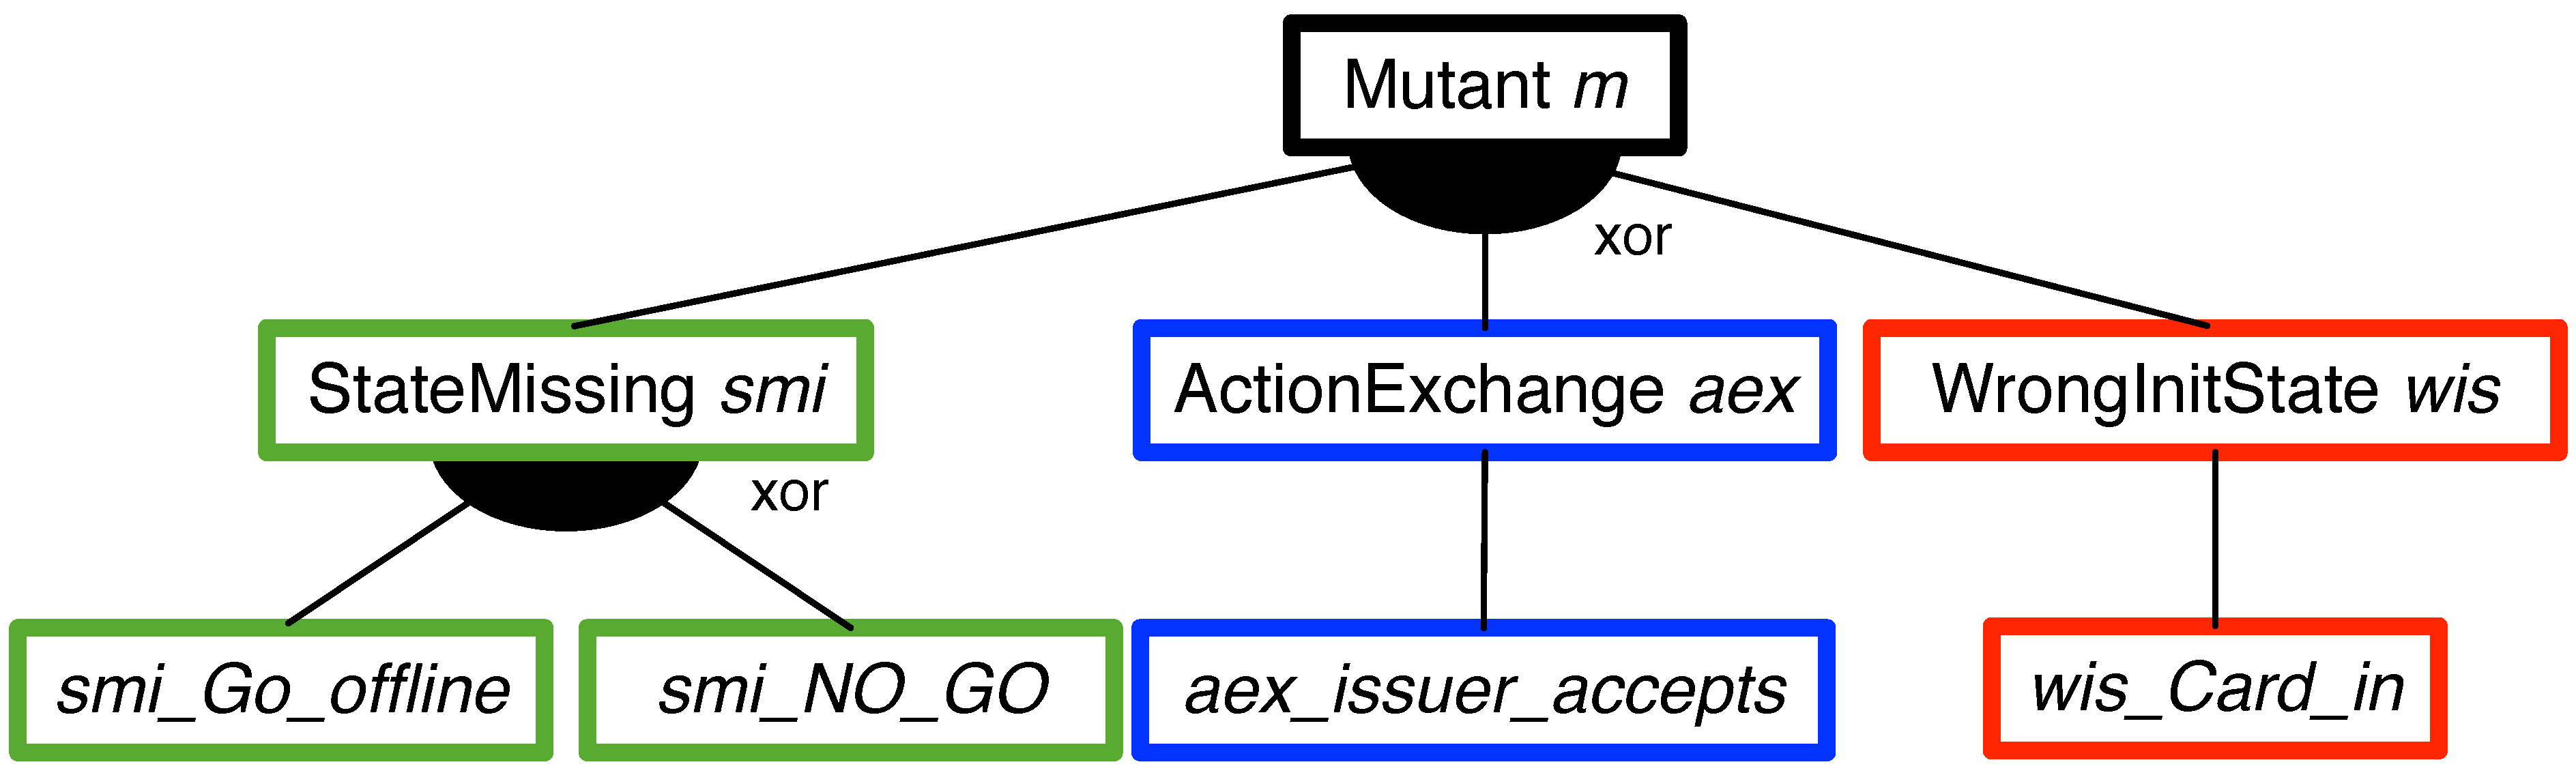
\includegraphics[width=85mm]{cpt-fmm-fm}
		\label{fig:fmm:cptmutantsfm}
	}
	\subbottom[Featured transition system]{
		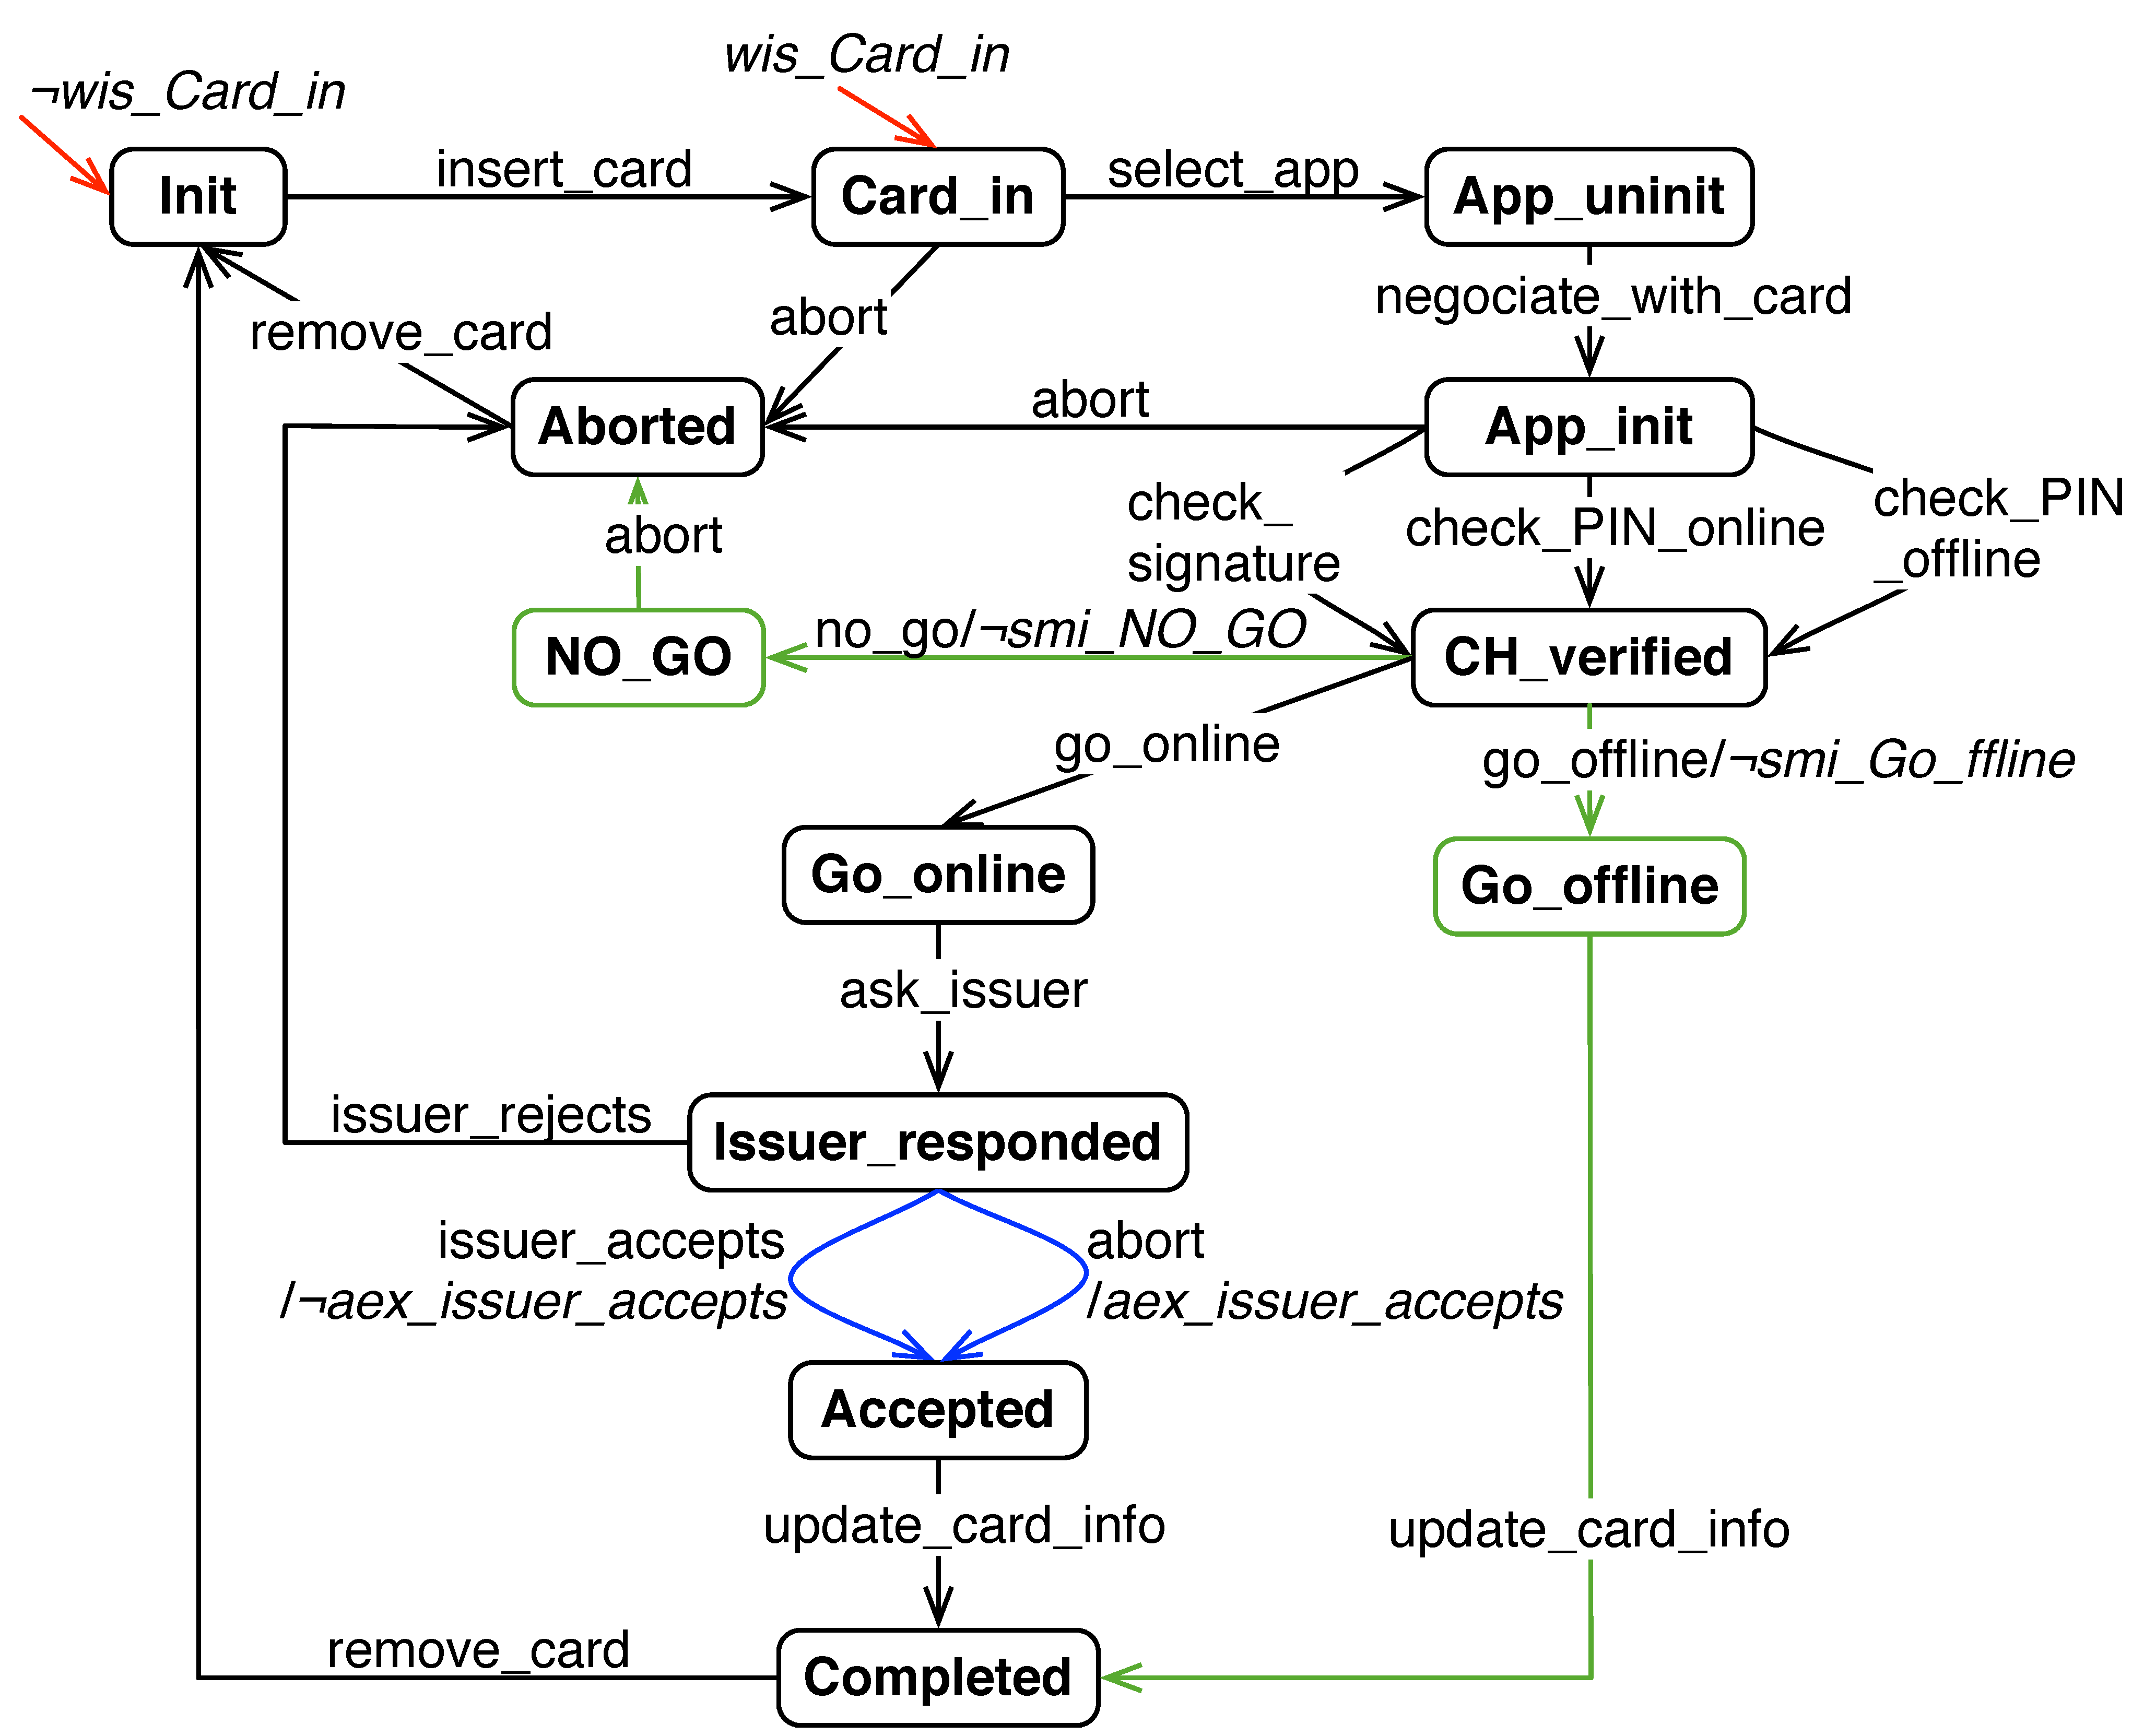
\includegraphics[width=85mm]{cpt-fmm-fts}
		\label{fig:fmm:cptmutantsfts}
	}
	\caption{Card payment terminal product FMM}
	\label{fig:fmm:cptmutantsfmm}
\end{figure}

To represent the variations introduced by the mutation operator (\ie the result of the application of the mutation operator) and the behaviour of the mutants, we use a feature model and an FTS. Each feature in the feature model represents a mutation of the LTS representing the behaviour of the system under test. When a member with one mutation (here represented as a feature) is selected and used with the projection operator on FTS, we obtain the behaviour (represented as a LTS) of the corresponding mutant. This allows us to embed all mutants in a single model, called the \acrfull{FMM}:
%
\begin{definition}[\acrfull{FMM}]
A \gls{FMM} is a couple \textit{(fts,fm)}, where \textit{fts} is an \gls{FTS} representing the behaviour of the original system and all the mutants of the family, and \textit{fm} is its associated \gls{feature model} where each feature represents a mutation of the original system. 
\end{definition}

For example, the FMM of Figure \ref{fig:fmm:cptmutantsfmm} has a feature model in Figure \ref{fig:fmm:cptmutantsfm} with 3 instances of mutation operators: the state missing  (\textit{SMI}) operator, which produces a mutant where one state is missing; the action exchange (\textit{AEX}) operator, which produces a mutant where one transition has its action changed (to another action); and the wrong initial state (\textit{WIS}) operator, which produces a mutant where the initial state has been set to another state. In this instance of the feature model, the SMI operator has been applied twice ($\mathit{smi\_go\_offline}$ mutant presented in Figure \ref{fig:fmm:cptsmi} and $\mathit{smi\_NO\_GO}$ mutant presented in Figure \ref{fig:fmm:cptsmi2}), and the AEX and WIS operators have been applied one time each ($\mathit{aex\_issuer\_accepts}$ mutant presented in Figure \ref{fig:fmm:cptaex} and  $\mathit{wis\_Card\_in}$ mutant presented in Figure \ref{fig:fmm:cptwis}). This feature model represents four first-order mutants, where at most one leaf feature is selected. The FTS in Figure \ref{fig:fmm:cptmutantsfts} represents all the possible variations, corresponding to the four mutation operators, of the original TS.

In order to derive one particular mutant from the FMM, one may use the FTS projection operator. Practically, this operator will first need a valid member of the mutant family, representing the desired mutant, \eg $p = \{m, \mathit{smi}, \mathit{smi\_Go\_offline}\}$; then, each feature expression of the FTS is evaluated with features belonging to the member replaced by true, and other features replaced by false; finally, transitions with a feature expression evaluated to false (\ie where $\gamma p = \mathit{false}$) and states that become unreachable are removed from the FTS. For instance, the projection of the FMM of Figure \ref{fig:fmm:cptmutantsfmm} on $p$ will produce the mutant LTS of Figure \ref{fig:fmm:cptsmi}.

To represent the effect of the WIS operator, we modify the FTS definition (Definition \ref{def:fts}) to replace the initial state $i$ by  a total function $init$ that indicates if a state of the FTS is the initial state of the system: 
%
\begin{definition}[\gls{FTS} for \gls{FMM}]
\label{def:fts4fmm}
A \gls{FTS} is a tuple $(S,$ $\Act,$ $\trans,$ $\mathit{init},$ $d,$ $\gamma)$, where:
\begin{itemize}
\item $S$, $\Act$, $\trans, d, \gamma$ are defined according to definition \ref{def:fts}; 
\item $\mathit{init}:  S \mapsto (\Sem{d} \mapsto \mathbb{B})$ is a total function indicating, for each state, for which product this state is the initial state and defined such that for every product there is exactly one initial state.
\end{itemize}
\end{definition}
%
To be compliant with existing tools, this modification is implemented using an artificial initial state $s_i$, such that for every product, there is an outgoing transition from $s_i$, with no label and a feature expression indicating that this transition may only be fired by this product, and going to the initial state of the product.


%-----------------------------------------------
\subsection{Building the featured mutants model} 
%-----------------------------------------------

\begin{figure}[t]
	\centering
	\subbottom[Enumerative approach]{
		\begin{tabular}{c c}
			\textbf{Input:} $lts$ & \textbf{Output:} $lts_m$ \\
			\begin{tikzpicture}[>=stealth',shorten >=1pt,auto,node distance=2cm]
			  \node[initial,state,initial text=] (s0)				 {$0$};
			  \node[state]         (s1) [right of=s0] {$s_1$};
			
			  \path[->] (s0)  edge node {a} (s1)
			        (s1) edge [bend left] node {a} (s0)
			         	 edge [loop below] node {b} (s1);
			\end{tikzpicture}
			& 
			\begin{tikzpicture}[>=stealth',shorten >=1pt,auto,node distance=2cm]
			  \node[initial,state,initial text=] (s0)				 {$0$};
			  \node[state]         (s1) [right of=s0] {$s_1$};
			
			  \path[->] (s0)  edge node {a} (s1)
			        (s1) edge [bend left] node {\textcolor{blue}{\textbf{b}}} (s0)
			         	 edge [loop below] node {b} (s1);
			\end{tikzpicture}
			\\
		\end{tabular}
		\label{fig:fmm:aexenumapproach}
	}\\
	\subbottom[FMM approach]{
		\begin{tabular}{c c}
			\textbf{Input:} $fts_{fmm}$ & \textbf{Output:} $fts'_{fmm}$ \\
			\begin{tikzpicture}[>=stealth',shorten >=1pt,auto,node distance=2cm]
			  \node[initial,state,initial text=] (s0)				 {$0$};
			  \node[state]         (s1) [right of=s0] {$s_1$};
			
			  \path[->] (s0)  edge node {a/$\gamma_1$} (s1)
			        (s1) edge [bend left] node {a/$\gamma_2$} (s0)
			         	 edge [loop below] node {b/$\gamma_3$} (s1);
			\end{tikzpicture}
			& 
			\begin{tikzpicture}[>=stealth',shorten >=1pt,auto,node distance=2cm]
			  \node[initial,state,initial text=] (s0)				 {$0$};
			  \node[state]         (s1) [right of=s0] {$s_1$};
			
			  \path[->] (s0)  edge node {a/$\gamma_1$} (s1)
			        (s1) edge [bend right=70] node [above] {a/$\neg \mathit{aex} \wedge \gamma_2$} (s0) 
					     edge [bend left] node {\textcolor{blue}{\textbf{b}}/$\mathit{aex}\wedge\gamma_2$} (s0)
			         	 edge [loop below] node {b/$\gamma_3$} (s1);
			\end{tikzpicture}
			\\
		\end{tabular}
		\label{fig:fmm:aexfmmapproach}
	}
	\caption{An example of mutation, the AEX operator}
	\label{fig:fmm:aexexample}
\end{figure}

We rely on the state-of-the-art operators proposed by Fabbri \etal \cite{Fabbri1999} to generate mutants from a LTS:
\begin{itemize}
\item[\emph{SMI}] State Missing operator: removes a state (other than the initial state) and all its incoming/outgoing transitions;
\item[\emph{WIS}] Wrong Initial State operator: changes the initial state;
\item[\emph{AEX}] Action Exchange operator: replaces the action linked to a given transition by another action;
\item[\emph{AMI}] Action Missing operator: removes an action from a transition, leaving an $\epsilon$-transition without action;
\item[\emph{TMI}] Transition Missing operator: removes a transition;
\item[\emph{TAD}] Transition Add operator: adds a transition between two states;
\item[\emph{TDE}] Transition Destination Exchange operator: modifies the destination of a transition.
\end{itemize}
%
Each operator can be used to generate mutants using the enumerative approach, where each mutant is formed as a new variation of the original LTS (possibly introducing non determinism in the case of AEX and TAD operators), or using the FMM approach, where each mutant is an addition to the feature model and the FTS. We detail hereafter the mutant generation procedures (the list of operators and the complete description of their effects is available in Appendix \ref{apdx:fmm:operators}).

\paragraph{Enumerative approach:}
%-------------------------------

\begin{algorithm}
	\KwIn{$\lts$: the original LTS to mutate;\\
		  $\mathit{Ops}$: the set of mutation operators to use;\\
		  $\mathit{times}: \mathit{Op} \rightarrow \mathbb{N}$: a function specifying for each operator the number of applications}
	\KwOut{$\mathit{muts}$, the set of produced mutants}
	\Begin{
		$\mathit{muts} = \emptyset $ \;
		\ForEach{$\mathit{op} \in \mathit{Ops}$}{
			\ForEach{$i \in [1 ; \mathit{times}(\mathit{op})]$}{
				$\mathit{muts} = \mathit{muts} \cup \mathit{op}(\mathit{random}(ts)) $ \; \nllabel{line:fmm:enumgen:mutgen}
			}
		}
  		\Return $\mathit{muts}$\;
	}
	\caption{Mutant generation, enumerative approach}
 \label{algo:fmm:enumgen}
\end{algorithm}

In the enumerative approach, each operator instance (\textit{op}) is defined as a model transformation with input a LTS (\textit{lts}) representing the behaviour of the product. It produces another (mutant) LTS ($\lts_m$) representing the result of this operator instance on $\lts$. For instance, AEX$(s_1, s_0, b)$, shown on Figure \ref{fig:fmm:aexenumapproach}, replaces  the action $a$ on transition $s_1 \overset{a}{\longrightarrow} s_0$ by \textcolor{blue}{$b$}. Algorithm \ref{algo:fmm:enumgen} details the enumerative approach where the set of mutants (\textit{muts}) is produced by applying each operator (in \textit{Ops}) with random parameters a number of times (defined for each operator by the \textit{times} function) on the original LTS (line \ref{line:fmm:enumgen:mutgen}).


\paragraph{FMM approach:}
%------------------------

In the FMM approach, an operator ($\mathit{Op}_{\fmm}$) is defined as a model transformation of a FMM (representing existing mutants), that produces a FMM representing (the previously existing mutants and) the result of the $\mathit{Op_{fmm}}$ mutation \emph{on the original TS} (obtained in the FMM's FTS by replacing the features by false in the feature expressions). 

For instance, in Figure \ref{fig:fmm:aexfmmapproach}, the AEX$_{\fmm}$ operator instance replaces the action $a$ on transition $s_1 \overset{a}{\longrightarrow} s_0$ of the base model by \textcolor{blue}{$b$} as follows: 
\begin{enumerate}
\item adding the feature expression $\neg \mathit{aex}$ on transition $s_1$ $\xrightarrow{a/\gamma_2}$ $s_0$, stating that $s_1$ $\xrightarrow{a/\neg \mathit{aex} \wedge \gamma_2}$ $s_0$ may be fired only if the $\mathit{aex}$ mutation is inactive (and if $\gamma_2$ is true);
\item adding a transition $s_1 \xrightarrow{b/ \mathit{aex} \wedge \gamma_2} s_0$, stating that the transition is fired with a $b$ action only if the $\mathit{aex}$ mutation is active (and if $\gamma_2$ is true);
\item adding an $\mathit{aex}$ feature to $fd_{fmm}$ representing the mutation done by $Op_{fmm}$ (not shown in Figure \ref{fig:fmm:aexfmmapproach}).
\end{enumerate}

\begin{algorithm}
	\KwIn{$\lts$: the original LTS to mutate;\\
		  $\mathit{Ops}$: the set of mutation operators to use;\\
		  $\mathit{times}: \mathit{Op} \rightarrow \mathbb{N}$: a function specifying for each operator the number of applications}
	\KwOut{$\fmm = (\fts_{\fmm}, \fm_{\fmm})$, the FMM}
	\Begin{
		$\gamma = (\lambda t \rightarrow \mathit{true})$ \; \nllabel{line:fmm:fmmmgen:fexprinit}
		$ \fts_{\fmm} = (S, \mathit{Act}, \mathit{trans}, i, \fm_{\fmm},\gamma)$ \; \nllabel{line:fmm:fmmmgen:fmminit}
		$ \fm_{\fmm} = (m) $ \; \nllabel{line:fmm:fmmmgen:fmmfminit}
		\ForEach{$\mathit{op} \in \mathit{Ops}$}{
			\ForEach{$i \in [1 ; \mathit{times}(\mathit{op})]$ \nllabel{line:fmm:fmmmgen:timesop} }{
				$\fmm = \mathit{op}_{\fmm}(\fmm) $ \; \nllabel{line:fmm:fmmmgen:mutgen}
			}
		}
  		\Return $\fmm$\;
	}
	\caption{Mutant generation, FMM approach}
 \label{algo:fmm:fmmgen}
\end{algorithm}

Algorithm \ref{algo:fmm:fmmgen} details the automated FMM building approach. We start with the original LTS and a $\gamma$ function that labels each transition with a true feature expression (line \ref{line:fmm:fmmmgen:fexprinit}). The feature model of the FMM is initialised to a root element $m$ (line \ref{line:fmm:fmmmgen:fmmfminit}). We then apply mutation operators ($\mathit{Ops_{fmm}}$) a specified number of times ($\mathit{times}(\mathit{op})$ line \ref{line:fmm:fmmmgen:timesop}). Contrary to the enumerative approach, the mutation operators are applied on the FMM under construction, which is reused in the next iteration (line \ref{line:fmm:fmmmgen:mutgen}). This is mandatory as the FMM contains all the previous mutations that are taken into account in the model transformations (\eg the $\gamma_{i}$ expressions in Figure \ref{fig:fmm:aexfmmapproach}). 
As we choose to only perform mutations on the original LTS, this forbids operator composition on (previously) mutated elements. Doing so ensures that first-order mutation maps to only one edit of the original LTS and that higher order mutants do not edit the same elements of the original LTS more than once.
Further details about the operators and specificities of the transformations can be found in Appendix \ref{apdx:fmm:operators}.

%-----------------------------------------------
\subsection{Featured mutants model execution}
%-----------------------------------------------

A test case for a product (\ie a LTS) is defined as a sequence of actions in this LTS (\textit{lts}), such that one execution form a path starting from and ending at the initial state (\textit{i}): $t=(\alpha_1, ..., \alpha_n) $ such that $ (i \overset{\alpha_1}{\longrightarrow} s_1, ..., s_{n-1} \overset{\alpha_n}{\longrightarrow} i)$.
Recall that in the enumerative approach, if a test case cannot be executed by the mutant (denoted $m \overset{t}{\nRightarrow}$) or does not end in the initial state of the original LTS (considered as the accepting state), it is considered  killed. Otherwise, the mutant is considered live. The set of live mutants, for $t$ in the set of mutants \textit{muts}, is defined as:
%
$$\mathit{liveEnum}(\mathit{muts}, t) = \{ m \in \mathit{muts} \mid m \overset{t}{\Longrightarrow} i  \} $$
%
In the FMM approach, a test case can be executed on an FMM \textit{fmm} (denoted $\fts_\mathit{{fmm}} \overset{t}{\Longrightarrow}$), if there exists at least one mutant or the product is able to execute it. 
The enumerative approach executes each test case on each mutant separately. In contrast, one execution of a test case on the FMM explores all the reachable mutants (identified by the collected feature expression $\gamma$).
The set of live mutants in the FMM approach is defined as:
%
$$\mathit{liveFMM}(\fmm, t) = \{ p \in [\![\fm_\mathit{{fmm}}]\!] \mid \fts_{\mathit{fmm} \mid p} \overset{t}{\Longrightarrow} i \}$$
%
Concretely, all possible paths in $\fts_\mathit{{fmm}}$ starting from $i$ and ending in $i$ will be considered, which allows to deal with possible non-determinism introduced by a mutation. The live mutants are those able to execute at least one of those paths, \ie those for which the product $p$ satisfies all the feature expressions on the transitions of the considered path.

For instance, the test case:
\begin{align*}
t =  & (\mathit{insert\_card}, \mathit{select\_app}, \mathit{negociate\_with\_card}, \mathit{check\_PIN\_offline},\\
 & \mathit{go\_offline}, \mathit{update\_card\_info}, \mathit{remove\_card})
\end{align*}
Executing the FMM of Figure \ref{fig:fmm:cptmutantsfmm}, it will fire the following transitions:
%
\begin{gather*}
( \xrightarrow{/\neg \mathit{wis\_Card\_in}} \mathit{Init},\\
 \mathit{Init} \xrightarrow{\mathit{insert\_card}} \mathit{Card\_in}, \\
 \mathit{Card\_in}  \xrightarrow{\mathit{select\_app}} \mathit{App\_uninit}, \\
 \mathit{App\_uninit} \xrightarrow{\mathit{negociate\_with\_card}} \mathit{App\_init}, \\
 \mathit{App\_init} \xrightarrow{\mathit{check\_PIN\_offline}} \mathit{CH\_verified}, \\
 \mathit{CH\_verified} \xrightarrow{\mathit{go\_offline}/\neg \mathit{smi\_go\_offline}} \mathit{Go\_offline}, \\
 \mathit{Go\_offline}  \xrightarrow{\mathit{update\_card\_info}} \mathit{Completed}, \\
 \mathit{Completed} \xrightarrow{\mathit{remove\_card}} \mathit{Init}) \\
\end{gather*}
%
These transitions may only be fired by mutants for which all the features expressions are $true$. Here, mutants need to respect the following constraint:
$$\neg \mathit{wis\_Card\_in} \wedge \mathit{\neg smi\_go\_offline}$$
All mutants in the feature model of Figure \ref{fig:fmm:cptmutantsfm} that satisfy this feature expression remain live after the execution of $t$. The set of mutants killed by the test case is computed using the conjunction of $\fm_{\fmm}$ and the negation of this feature expression: $\fm_{\fmm} \wedge (\mathit{wis\_Card\_in} \vee \mathit{smi\_go\_offline})$, which corresponds to the set of mutants: 
$$\left\lbrace(m, \mathit{wis}, \mathit{wis\_Card\_in}), (m, \mathit{smi}, \mathit{smi\_go\_offline}) \right\rbrace$$

In practice, $\mathit{liveFMM}(\fmm, t)$ produces a feature expression representing all the live mutants as detailed in Algorithm \ref{algo:fmm:livefmm}. Initially, the algorithm computes all the paths in $\fts_\mathit{{fmm}}$ corresponding to the sequence of actions in $t$ (line \ref{line:fmm:livefmm:paths}). For one path, the conjunction of the feature expressions gives the mutants able to execute this path (line \ref{line:fmm:livefmm:disjunct}). Effort is saved this way by ignoring unreachable mutants and by sharing the execution of the common transitions. This conjunction disjuncts with the conjunctions of the others paths to get the feature expression representing all the live mutants (line \ref{line:fmm:livefmm:disjunct}). This step results in savings due to merging of the considered executions. For performance reasons, the $\mathit{paths}$ variable uses a tree representation to merge common prefixes of different paths.

\begin{algorithm}
	\KwIn{$\fmm = (\fts_{\fmm}, \fm_{\fmm})$, the FMM;\\
		  $t = (\alpha_1, ..., \alpha_n)$: a test case defined over the original LTS}
	\KwOut{$\mathit{live}$, the feature expression representing the mutants live after executing $t$ on $\fmm$}
	\Begin{
		$\mathit{live} = false$ \;
		$\mathit{paths} = \{ (i \overset{\alpha_1 / \gamma_1}{\longrightarrow}\ldots \overset{\alpha_n / \gamma_n}{\longrightarrow} i) \} $ \; \nllabel{line:fmm:livefmm:paths}
		\ForEach{$p \in \mathit{paths}$}{
			$ \mathit{live} = \mathit{live} \vee (\bigwedge_{\gamma_i \in p} \gamma_i)$ \nllabel{line:fmm:livefmm:disjunct}
		}
  		\Return $\mathit{live}$\;
	}
	\caption{FMM mutant execution}
 \label{algo:fmm:livefmm}
\end{algorithm}

We implemented the different mutant operators described in Appendix \ref{apdx:fmm:operators} in order to perform classical mutation testing (enumerative approach) as well as FMM generation and execution in VIBeS, our Variability Intensive Behavioural teSting Java framework.


%-----------------------------------------------
\subsection{FMMs as higher order mutants model}
%-----------------------------------------------

Higher order mutants can be valuable since some of them tend to be hard to kill \cite{Harman2014}. However, the number of mutants grows exponentially according to the order $n$ and explodes the involved cost. This is obvious in Algorithm \ref{algo:fmm:enumgen}, for the enumerative approach, which generates all the $n-1$ mutants to generate the $n$th-order ones.

Using the FMM approach, modelling higher order mutation comes at (nearly) no cost. In a FMM ($\fts_{\fmm}, \fm_{\fmm}$), the set of allowed mutants (\ie variations in $\fts_{\fmm}$) is represented by the feature model ($\fm_{\fmm}$). For instance, the constraints in the $\fm_{\fmm}$ of Figure \ref{fig:fmm:cptmutantsfm} allows to have exactly one mutant at a time. Meaning that all valid mutants (members) of this FMM will have at most one variation from the original LTS made by a mutation operator, \eg Figure \ref{fig:fmm:cptsmi} has (only) $\mathit{smi\_go\_offline}$ feature active. 

\begin{figure}[h]
	\centering
	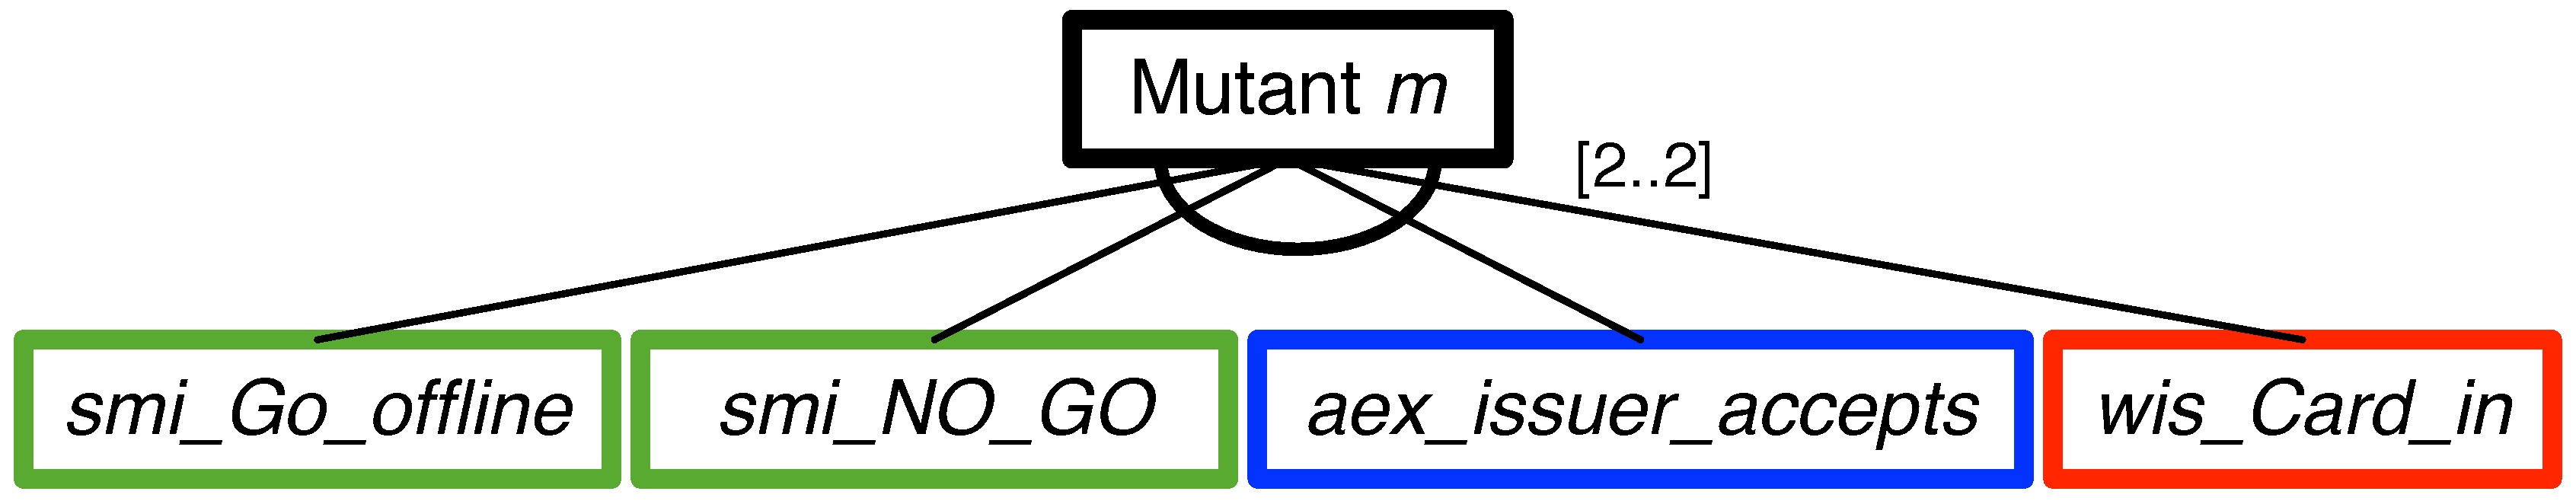
\includegraphics[width=85mm]{cpt-fmm-order2-fm}
	\caption{The order 2 FMM of the card payment terminal example}
	\label{fig:fmm:order2fmm}
\end{figure}

The $n$th order mutants are represented by modifying the constraints on the $\fm_{\fmm}$ so that they have exactly $n$ mutations at a time. It means that generating the FMM using Algorithm \ref{algo:fmm:fmmgen} will also generate the FTS (which will be the same) for order 1 to $n$ FMMs. For instance, the card payment terminal product has the same FTS, for all orders as shown in Figure \ref{fig:fmm:cptmutantsfts}, but differs on the feature model that is described by Figure \ref{fig:fmm:order2fmm} by the group cardinality stating that exactly 2 subfeatures have to be selected. The FMM will compactly represent all the $C^{4}_{2} = 6$ 2nd-order mutants.

\paragraph{All-order mutants:} 
%-----------------------------

Using the same argument, we generalize to mutants of any order by setting the group cardinalities of the feature model in Figure \ref{fig:fmm:order2fmm} to  $[1..4]$. In this case, the FMM represents a single model with all possible orders of mutants (with $n$ between 1 and the number of leaf features in the FMM's feature model). A valid member (mutant) of the feature model will contain at least one application of a mutation operator,\eg a mutant $m = \{m,$ $\mathit{smi\_go\_offline}\}$, but also  $m' = \{m,$ $\mathit{smi\_go\_offline},$ $\mathit{smi\_NO\_GO}\}$, or $m'' = \{m,$ $\mathit{smi\_go\_offline},$ $\mathit{wis\_Card\_in}\}$, \etc In this case, the FMM compactly represent all the $2^{4} - 1 = 15$  $n$-order mutants.

The number of live mutants after the execution of a test case ($t$) on a FMM ($\fmm$) can be obtained by counting the number of SAT solutions (\ie the number of possible assignments for each feature) to $\fm_{\fmm} \wedge \mathit{liveFMM}(\fmm, t)$, where $\fm_{\fmm}$ is the FMM feature model encoded as a boolean formula, \ie the disjunction of the mutations ($\mathit{Ops}$): $\fm_{\fmm} = \bigvee_{o \in \mathit{Ops}} o$. For a test set ($s$), the number of live mutants is computed by counting the number of SAT solutions to
%
$$ \left(\bigvee_{o \in \mathit{Ops}} o \right) \wedge \left(\bigwedge_{t \in s} \mathit{liveFMM}(\fmm, t) \right). $$


%%%%%%%%%%%%%%%%%%%%%%%%%%%%%%%%%%%%
\section{Equivalent mutants problem}
%%%%%%%%%%%%%%%%%%%%%%%%%%%%%%%%%%%%

\label{sec:EMP}

\glsreset{EMP}

Despite its potential, mutation analysis faces a number of challenges that currently prevent wider adoption \cite{Papadakis2015, Jia2011a}. One of them is the \textit{\gls{EMP}}. It concerns the mutants whose behaviour is identical to the original artefact (code or model). Such mutants cannot be distinguished by any test case, a situation that raises two issues: 
\begin{inparaenum}
\item they hamper the use of the criterion as a stopping rule by skewing the mutation score measurement (the number of killed mutants divided by the total number of mutants); and
\item they do not bring any new value to the test selection techniques as they attempt to kill mutants that have no chance to be killed. 
\end{inparaenum}

Mutant equivalence  can take two forms \cite{Papadakis2015}: 
\begin{inparaenum}
\item equivalence between mutants and the original system; \label{item:equivmutants}
\item equivalence between two mutants (not with the original system). \label{item:duplmutants}
\end{inparaenum}
Mutants of case (\ref{item:equivmutants}) are called \emph{equivalent} while mutants of case (\ref{item:duplmutants}) are called \emph{duplicate}. We focus here on mutants that are behaviourally equivalent to the original system, \ie mutants of case (\ref{item:equivmutants}).   

%-----------------------------------------
\subsection{\gls{EMP} and automata theory}
%-----------------------------------------

\glsreset{ALE}

The model-based formulation of the \gls{EMP} can be expressed as a classical problem in automata theory: \emph{\gls{ALE}}. The accepted language of an automaton is formed by all the sequences of actions (words)  that can be accepted \ie starting in the initial state and ending in a final state. Therefore, if a mutant $m$ accepts the same language as the original $o$ (\ie is language-equivalent to the original), then there is no test sequence $s$ that can distinguish the mutant from the original:
$$ \forall s, s \in \mathcal{L}(o) \Leftrightarrow s \in \mathcal{L}(m)$$

There are various relations defined between two automata that we can compute to determine whether they are language-equivalent. Among them, we can cite bisimulations or trace equivalence \cite{Baier2008}. In the last years, the verification community came up  with dedicated relations concepts such as bisimulations up to congruence \cite{Bonchi2013} or antichains \cite{Doyen2010} to address language equivalence.  In model-based mutation testing, Aichernig \etal investigated  language inclusion (but not equivalence) using refinement checking \cite{Aichernig2015} in order to select mutant-killing test cases.  

Although tackling the language equivalence and inclusion problems from different angles and heuristics, all these techniques may face exponential blow-up since both language inclusion and equivalence were demonstrated to be PSPACE complete \cite{Kupferman1996}. While worst-case complexity can seem discouraging, various heuristics have been proposed to limit the effects of this complexity in practice.  One of our goals is to determine the applicability of an exact language equivalence algorithm to address the EMP \cite{Bonchi2013}. The algorithm selected due to its availability, reported performance over the state of the art and ability to handle non-determinism that mutations may incur. In the next section, we also present two baseline algorithms that run generated traces to distinguish original and mutants' behaviours.

%-----------------------------------------
\subsection{Strong and weak mutation}
%-----------------------------------------

J{\"o}bstl \cite{Jobstl2014} discussed the conditions, identified by DeMillo and Offutt \cite{DeMillo1993}, that must be fulfilled to kill a mutant:
\begin{enumerate}
\item ``the \emph{necessity condition} says that the state of the mutated program after some execution of the mutated statement must be incorrect with respect to the original program. This implies that the mutated statement must be reached. This is necessary, but not sufficient'';
\item ``the \emph{sufficiency condition} says that the final state of the mutant must differ from the final state of the original program, \ie the necessary incorrect intermediate state must propagate to an incorrect final state.''
\end{enumerate}
Satisfying the necessity condition  alone is referred to as \emph{weak mutation}, while satisfying both is \emph{strong mutation} \cite{Howden1982,Mathur2008}. 

\glsreset{WM} \glsreset{SM}

At the model level, our simulations detect an incorrect state if an abstract test case that is valid with respect to the original LTS, is invalid on the mutant LTS, or vice-versa. Indeed, when executed, an abstract test case induces one or more \textit{runs} (alternating sequences of states and actions), depending on the presence of non-determinism. If one run does not contain all the actions of the abstract test case (\ie the run is \emph{incomplete}), it is because of the presence of an incorrect state preventing the subsequent actions to be fired. If all runs are complete, the original and the mutant are assumed equivalent for this test case. 
Necessity and sufficiency conditions affect the final states of these runs. For \gls{WM}, these states can map to any state of the LTS (like for abstract test cases). For \gls{SM}, we need to account for the fact that LTSs have no final states: in this case, we assimilate the initial state to a final state and consider only positive (or negative) abstract test cases for strong mutation.

The \gls{ALE} approach uses automata that have explicit initial and final states. For weak mutation, we generate automata in which all states are final, and for strong mutation the initial state is the only final state.

%-----------------------------------------
\subsection{Mutant equivalence analysis}
%-----------------------------------------

\glsreset{RS} \glsreset{BS}

As explained in the previous sections, equivalent mutant detection may be done using automata language equivalence. Since this is a PSPACE complete problem, we also propose two randomized approaches: \emph{\gls{RS}} and \emph{\gls{BS}}. Those approaches are straightforward:  we generate random (either fully random or biased random) traces from the original (resp. mutant) model and run them on the mutant (resp. original) model. If a trace fails to execute on one of the models, it serves as a counterexample and disproves equivalence.  Otherwise, the mutant is considered \emph{probably equivalent} and testers have to decide whether they want to perform more simulations or switch to an exact method. 

\paragraph{Automata language equivalence:}
%-----------------------------------------

The \gls{ALE} approach we selected for comparison is developed by Bonchi and Pous \cite{Bonchi2013}. It can be thought of as an extension to non-deterministic LTSs of the Hopcroft-Karp algorithm. In particular, they introduce a bisimulation relation called \emph{up to congruence} that requires to explore less states than the original algorithm. This approach also avoids to build the complete deterministic finite TS and performs determinisation on-the-fly. This makes such an approach particularly relevant: non-determinism may be introduced locally by mutations (our original models are deterministic), thereby limiting determinisation scope\footnote{This is indeed the case in our evaluation: between 0\% and 15.5\% of the mutants are non-deterministic (see Section \ref{sec:experiment:mutequiv}).}.

\paragraph{Randomized simulations:}
%-----------------------------------------

\newcommand{\wValid}{\mathit{valid}}
\newcommand{\wInvalid}{\mathit{invalid}}
\newcommand{\wTraceset}{\mathit{traceset}}
\newcommand{\wSelect}{\mathit{select}}
\newcommand{\wNone}{\mathit{none}}

\begin{algorithm}
	\KwIn{$o$, the original LTS;\\
		  $m$, the mutant to compare to $o$; \\
		  $N$, the total number of traces to generate;\\
		  $k$, the length of the abstract test cases;
		 }
	\KwOut{$t$, an abstract test case differentiating $m$ from $o$ or $\wNone$ if $m$ is potentially equivalent to $o$.}
	\Begin{
		$\wTraceset = \wSelect(o, \dfrac{N}{2}, k)$ \; \nllabel{line:fmm:randomequiv:posrandomselect}
		\ForEach{$t \in \wTraceset$}{
			\If{$\neg (m \overset{t}{\Longrightarrow})$ \nllabel{line:fmm:randomequiv:posexec}}{
				\tcp{mutant fails to execute $t$, returns $t$}  
				\Return $\wValid(t)$ \; \nllabel{line:fmm:randomequiv:returnpos}
			}
		}
		$\wTraceset = \wSelect(m, \dfrac{N}{2}, k)$ \; \nllabel{line:fmm:randomequiv:negrandomselect}
		\ForEach{$t \in \wTraceset$}{
			\If{$\neg (o \overset{t}{\Longrightarrow})$ \nllabel{line:fmm:randomequiv:negexec}}{
				\tcp{original LTS fails to execute $t$, returns $t$} 
				\Return $\wInvalid(t)$ \; \nllabel{line:fmm:randomequiv:returnneg}
			}
		}
  		\Return $\wNone$\; \nllabel{line:fmm:randomequiv:return}
	}
	\caption{Mutant equivalence analysis: generic randomized simulation}
 \label{algo:fmm:randomequiv}
\end{algorithm}

Algorithm \ref{algo:fmm:randomequiv} presents our generic randomized simulation approach: $N$ abstract test cases are selected (respectively) from the original model (line \ref{line:fmm:randomequiv:posrandomselect}) and the mutant model (line \ref{line:fmm:randomequiv:negrandomselect}), and executed (respectively) on the mutant model (line \ref{line:fmm:randomequiv:posexec}) and the original model (line \ref{line:fmm:randomequiv:negexec}).  In case of non deterministic behaviour, all the possible paths are considered for the execution of the abstract test case. If one equivalence test fails, the algorithm stops and returns an abstract test case, either valid for the original LTS (line \ref{line:fmm:randomequiv:returnpos}), such as 
$$(o \overset{t}{\Longrightarrow}i) \wedge \neg (m \overset{t}{\Longrightarrow}i)$$ 
or an abstract test case, invalid for the original LTS (line \ref{line:fmm:randomequiv:returnneg}), such as 
$$\neg (o \overset{t}{\Longrightarrow}i) \wedge (m \overset{t}{\Longrightarrow}i)$$

This generic simulation algorithm is instantiated through two strategies for trace generation (lines \ref{line:fmm:randomequiv:posrandomselect} and \ref{line:fmm:randomequiv:negrandomselect}): \acrfull{RS} and \acrfull{BS}. The parameter $N$ is computed using the Chernoff-Hoeffding bound.

\paragraph{Random simulation:}
%-----------------------------

Random simulation assumes a uniform distribution of on the transitions enabled in each state, that is, such abstract test cases are selected randomly ($\wSelect$ call on lines \ref{line:fmm:randomequiv:posrandomselect} and \ref{line:fmm:randomequiv:negrandomselect} in Algorithm \ref{algo:fmm:randomequiv}) by accumulating the actions $\alpha_i$ triggered by a random walk of a given length $k$ in the LTS. For weak mutation (\gls{WM} \gls{RS}), the only constraint is to start the random walk from the initial state $i$. Strong mutation (\gls{SM} \gls{RS}) requires a random walk starting from and ending in $i$\footnote{After few tries, this method (\ie using a random walk until the initial state $i$ is reached) showed very poor results on our largest models (we set a timeout of one hour for one equivalence detection) and is therefore not further discussed. See Section \ref{sec:experiment:mutequiv} for more details.}.


\paragraph{Biased simulation:} 
%----------------------------

The \acrfull{BS} approach exploits the basic characteristics of mutation testing: mutations are localised and they create (most of the time) behavioural differences. It assumes that those differences are detected by an abstract test case $t$ which, when executed on the original LTS $o$ or on its mutant $m$, goes through one of the states affected by the mutation. For instance, the \textit{transition missing operator} produces a mutant by removing a transition $a\overset{\alpha_i}{\longrightarrow}b$ from the original LTS. The \gls{BS} approach (that does not know which mutation has been performed) selects abstract test cases in $o$ and $m$, such that their executions $m \overset{t}{\Longrightarrow}$ or $o \overset{t}{\Longrightarrow}$ reach $a$ or $b$ (where a syntactic difference between the models is detected).  Such states, called \emph{infected states}, have been shown to help identifying equivalent mutants at the code level \cite{Offutt1997,Bardin2015} and to speed up mutation analysis at the model level \cite{Krenn2016}. This motivates us to adopt this strategy in our biased simulation.  

In practice, the set of infected states $S_{\mathit{infect}}$ is computed by checking syntactic differences between the original and mutant LTSs. It will include: 
\begin{enumerate}
\item connected states (\ie states accessible from the initial state) from one model which are not present in the other, 
and
\item states with differences in their input/output transitions: in number of transitions or in action names, considering any pair of states $<s_o,s_m>$ where $s_o$ is a state in the original TS, $s_m$ a state in the mutant TS, such that their names are identical. 
\end{enumerate}
An alternative is to instrument the mutant generator to keep track of the list of infected states while generating the mutants. Our goal is to be able to apply this strategy without any information on how the mutants are generated (\eg generated by other frameworks than ours) and to fairly compare  with an exact approach  that makes no assumption on the locality of differences. Once the set of infected states  $S_{\mathit{infect}}$ is obtained (by any means), the second step is to generate traces that cover such infected states.

For weak mutation (\gls{WM} \gls{BS}), an abstract test case $t$ is selected ($\wSelect$ call on lines \ref{line:fmm:randomequiv:posrandomselect} and \ref{line:fmm:randomequiv:negrandomselect} in algorithm \ref{algo:fmm:randomequiv}) by concatenating the actions of the shortest walk from the initial state $i$ to a randomly chosen state $a \in S_{\mathit{infect}}$ and a random walk starting from $a$. To proceed, the first step during abstract test case selection is to compute the shortest distance (\ie the number of transitions) between each state of the original LTS $o$ (or its mutant $m$ respectively) and the initial state $i$ of $o$ (or $m$ respectively) using a standard breadth-first search \cite{Cormen2001}. 

For strong mutation (\gls{SM} \gls{BS}), instead of a random walk starting from $a$, the algorithm will consider the actions of a path starting from $a$ and returning to $i$ using the computed shortest distance: the distance from $a$ to $i$ will (not strictly) decrease each time a transition is taken in the path.

\paragraph{Estimating the number of required runs:}
%-------------------------------------------------

An important parameter for simulation is the number of abstract test cases selected from the original (resp. mutant) model and run on the mutant (resp. original) model: $N/2$. Under the hypothesis that abstract test cases are uniformly distributed we can bound the equivalence probability and estimating the number of runs needed achieve these bounds. Herault \etal \cite{Herault2004} suggested to use the Chernoff-Hoeffding bound to estimate the number $N/2$ of required runs to limit the equivalence probability depending on the approximation parameter $\epsilon > 0$ and a confidence parameter $\delta < 1$. If $N/2 \geq \frac{4\log(2/\delta)}{\epsilon^2} $ then we have: 
$$Pr \left[ equiv(m,o) \right] = Pr\left[ \left| \frac{A}{N/2}-p \right| \leq \epsilon \right] \geq 1-\delta$$
Where $A$ is the number of successful runs that is either $m \overset{t}{\Longrightarrow}$ or $o \overset{t}{\Longrightarrow}$ for a given abstract test case $t$.  In practice, we compute $2A/N$ only when the algorithm has exhausted all the runs and set $N=\frac{8\log(2/\delta)}{\epsilon^2}$ for the number of runs as we have to account for two-way simulation (\ie two simulations): the number of runs is thus doubled. 

It has to be observed that regarding biased simulations, the distribution of abstract test cases will not be uniform as the infected states force abstract test cases to explore only given portions of the model, \viz where the mutations are. Although this inequality may not hold in this case, we alleviate this threat by not trying to interpret the $\delta$ and $\epsilon$ values for biased simulations: they are for us a convenient means to compute $N$. Furthermore, keeping the same number of runs for random and biased simulations allows comparing their execution times and recalls (See Section \ref{sec:experiment:mutequiv}).


%%%%%%%%%%%%%%%%%%%%%%%%%%%%%%%%
\section{Related work}
%%%%%%%%%%%%%%%%%%%%%%%%%%%%%%%%

Program mutation was proposed as a rigorous testing technique \cite{Budd1980}. The idea was then applied to test specification models \cite{Offutt2011} and recently to resolve software engineering problems such as the improvement of non-functional properties \cite{Langdon2015}, locating \cite{Papadakis2015a} and fixing software defects \cite{LeGoues2012}. Here we briefly discuss works related to model-based mutation and code-based mutation.

%----------------------------------
\subsection{Model-based mutation}
%----------------------------------

The idea of model-based mutation has been elicited by Gopal and Budd \cite{Budd1985} who called it \textit{Specification Mutation}. Specification mutation promises to identify defects related to missing functionality and misinterpreted specifications \cite{Budd1985}. This is desirable since these kinds of defects cannot be identified by any code-based testing technique \cite{Howden1976,Voas1997}, including code-based mutation. 

Gopal and Budd \cite{Budd1985} studied mutation for specifications expressed in logic. Similarly, Woodward \cite{Woodward1993} mutated and experimented with algebraic specifications. Mutating models like finite state machines and Statecharts has also been done by Fabbri \etal \cite{Fabbri1999b}. Hierons and Merayo \cite{Hierons2009} used Probabilistic Finite State Machines. All these studies suggested a set of operators and report some exploratory results.  Amman \etal \cite{Ammann1998} suggested comparing the original and the mutated specification models using a model checker in order to generate counterexamples. These can then be used as test cases for the system under test. Black \etal \cite{Black2000} defined a set of operators based on empirical and theoretical analysis. They also defined a process of using them based on the SMV model checker. Contrary to our approach, none of these methods considers the mutation efficiency.

Recent research focuses on mutating behavioural models. Aichernig \etal \cite{Aichernig2014a,Aichernig2015,Aichernig2014} defined UML state machines mutant operators and used them to insert faults in the models of an industrial system. These were used to design tests. The approach has a formal ground but neither considers optimising the test execution, nor higher order mutation. 
Belli and Beyazit \cite{Belli2006,Belli2011d} compare event-based and state-based model mutation testing. Both approaches were found to have similar fault detection capabilities. The authors also report that it seems more promising to perform higher order mutation than first-order mutation but did not provide evidence in support of this argument. Krenn \etal \cite{Krenn2015} made available their MoMuT tool, but it is dedicated to test selection and not mutant execution or equivalent mutant detection as our approach. In their most recent work \cite{Krenn2016}, they use an idea similar to FMM by triggering mutations during exploration of the model, avoiding execution of similar prefixes in different mutants. Additionally, MoMuT does not support higher order mutation. Recently, Granda \etal \cite{Granda2016} defined mutation operators for UML class diagrams.

Other applications of model-based mutation are to test model transformations and test configurations. Mottu \etal \cite{Mottu2006} defined a fault model relevant to the model transformation process based on which they propose a set of mutant operators.
Finally, Papadakis \etal \cite{Papadakis2014} demonstrated that model-based mutation of the combinatorial interaction testing models has a higher correlation with the actual fault detection than the use of combinatorial interaction testing. Thereby, they provide ground to the argument that model-based mutation might be more effective than the other model-based testing methods. 

%----------------------------------
\subsection{Code-based mutation}
%----------------------------------

In the context of code-based mutation, executable mutants are needed. This introduces a compilation overhead which is proportional to the number of mutants. To reduce this cost, Untch \etal \cite{Untch1993} proposed mutant schemata, an approach that replaces the program operators with schematic functions. These functions introduce the mutants at runtime and thus, only one compilation is needed. Ma \etal \cite{Ma2005} suggested using bytecode translation, a technique that introduces the mutants directly at the bytecode level and thus avoid multiple compilations. 

To reduce the test execution overhead, several optimizations have been proposed. Delamaro and Maldonado \cite{Delamaro2001} suggested recording the execution trace of the original program and consider only the mutants that are reachable by each of the employed tests. Along the same lines, Mateo and Polo \cite{Mateo2014} suggested stopping mutant executions when they cause infinite loops. Jackson and Woodward \cite{Jackson2001} suggested parallelizing the mutant execution process. Kapoor and Bowen \cite{Kapoor2004} proposed ordering the mutants in such a way that the test execution is minimized. Papadakis and Malevris \cite{Papadakis2011} used mutant schemata to identify mutants that are reached and infected by the considered tests. They then reduce test execution by considering only the mutants that cause infection. This technique was later evaluated by Just \etal \cite{Just2014a} who found that it reduces test execution by 40\%. 

%-------------------------------------------------------------
\subsection{\gls{SPL} and other variability models mutation}
%-------------------------------------------------------------

Henard \etal \cite{Henard2013b,Henard2014} and Arcaini \etal \cite{Arcaini2015a,Arcaini2016a} define mutant operators for feature models and use them to assess the ability of a set of products (\ie a test suite in their case) to find faults. Along the same lines, Lackner and Schmidt \cite{Lackner2014} define mutant operators for the mappings of features with other model artefacts, and Al-Hajjaji \etal \cite{Al-Hajjaji2016b} define mutation operators for preprocessor-based variability. Arcaini \etal \cite{Arcaini2017} also mutated feature models in order to detect anomalies software artefacts \cite{Arcaini2017}. Finally, Henard \etal \cite{Henard2014}, Reuling \etal \cite{Reuling2015a}, Matnei Filho and Vergilio \cite{MatneiFilho2016} mutate the feature model to select products to test. 

%----------------------------------------
\subsection{Mutant equivalence analysis}
%----------------------------------------

Previous work demonstrated that equivalent mutants skew the mutation score measurements and thus hinder the effectiveness of the method \cite{Madeyski2014}. Unfortunately, it has been proven that judging whether a code mutant is equivalent to the original code is an undecidable problem \cite{Budd1982}. This means that there is no solution to the general case of this problem. Luckily, since mutations are small syntactic changes, heuristics can identify several classes of them \cite{Papadakis2015}. Two types of such heuristics exist in the literature: those that operate in a static manner and those that are dynamic. 

Static techniques include the use of compiler optimizations \cite{Offutt1994}, constraint solving \cite{Offutt1997}, program slicing \cite{Hierons1999}, data-flow patterns \cite{Kintis2015}, and formal verification \cite{Bardin2015}. All these techniques are effective at detecting certain types of equivalent mutants, \ie trivial equivalences \cite{Papadakis2015}, but unfortunately, they are not applicable to model mutants.

Dynamic techniques measure the differences between the test executions of the original and mutant programs and identify likely non-equivalent mutants. Schuler and Zeller \cite{Schuler2013} and Papadakis \etal \cite{Papadakis2014a} measure the impact on coverage, while Kintis \etal \cite{Kintis2015a} measure the impact on other mutants (second-order mutants). Our technique shares the same notion of equivalence because we check the model trace in order to judge it. However, we do not consider executable code as we only deal with model mutants. We also sample execution in order to increase the efficiency of the process. It is to be noted that we have a different notion of equivalence since we deal with behavioural models. Therefore, differences in traces imply different behaviours, which is not the case for executable code.

Non-determinism complicates equivalence detection both at the code \cite{Patel2016} and model levels \cite{Aichernig2012}. Patel and Hierons \cite{Patel2016} associate predictions from pairs of inputs and outputs of the mutant program and check whether these predictions can be discarded by the original program, hence showing non-equivalence. This is not applicable to our case since our models do not have outputs. Aichernig and J{\"o}bstl \cite{Aichernig2012} also encode the semantics of the action models in terms of constraints and use refinement to check conformance in the context of non-determinism. In our case, RS/BS manage non determinism in the TSs by considering all the possible runs. 

Perhaps the closest work is that of Papadakis and Malevris \cite{Papadakis2012} who sample execution paths according to their length (select the k-shortest paths), symbolically execute them and judge mutant equivalence based on the selected paths. The main differences with our approach are that we additionally sample paths that cover infected states and we operate on behavioural models instead of actual code representation.  


%%%%%%%%%%%%%%%%%%%%%%%%%%%%%%%%%%%%
\section{Wrap up}
%%%%%%%%%%%%%%%%%%%%%%%%%%%%%%%%%%%%

In this chapter we discuss our contributions to model-based mutation analysis to: 
\begin{inparaenum}
\item generate, represent, and effectively execute mutants using a family-based approach to model-based mutation testing, named \acrfull{FMM}; and
\item tackle the equivalent mutant problem at the model level using an exact language equivalence (called \acrfull{ALE}) and two random simulations approaches (called \acrfull{RS} and \acrfull{BS}).
\end{inparaenum}

\paragraph{Compact mutant model:}
%---------------------------------

\emph{\gls{FMM}} takes advantage of the variability formalisms (\textit{i.e.,} FTS and feature model) to compactly represent all possible mutations on a single model. To do so, we rely on modelling the behaviour of the product under test and view mutant operators as model transformations that can be activated on demand by selecting features in the feature model of the FTS. It allows to generate mutants of any order and assess test effectiveness via an optimised execution scheme. Testing behavioural models with FMM is a completely automated process that involves no extra manual or computational effort over previous approaches. 

In short, the use of FMM has the following \emph{benefits}: first, it can easily reason about and \emph{generate behavioural mutants}; second, it can significantly \emph{speed up} the evaluation of test suites against mutants (up to 1,000 times, as showed in Section \ref{sec:experiment:fmmexec}); and finally, it can efficiently perform \emph{higher order mutation}. 

\paragraph{Equivalent mutant problem:}
%------------------------------------

To tackle the \emph{\acrfull{EMP}} at the model level, we offer two baseline algorithms based on random simulation, and compare them to language equivalence under \emph{weak} and \emph{strong} mutation scenarios. Our experiments in Section \ref{sec:experiment:mutequiv} demonstrates the efficiency of the exact approach for the weak mutation scenario. For strong mutation, our biased simulations, that pre-process the models to detect  states that are infected by mutations, are efficient (up to 1,000 times faster) on models that contain more than 300 states, limiting detection errors to 8\%. This suggests using \emph{simulations first} to quickly discard many non-equivalent mutants, and then employing \emph{exact approaches} only on a small amount of probably equivalent mutants to speed up equivalence analysis.      

There is room for improvement. First, we will extend our experiments to other forms of equivalence and tools: for instance, the usage of a random based simulation directly in the FMM to quickly filter out non equivalent mutants. We would also like to switch from the pure equivalence analysis to test selection concerns by analysing counter-examples. Our long-term goal is to draw attention on the applications of language equivalence for mutation testing and develop further EMP-dedicated solutions.      






\chapter{Empirical assessment}
\label{chap:assessment}


This chapter presents the empirical assessment performed to validate the test suite selection criteria described in Chapter \ref{chap:coverage} and the mutation analysis described in Chapter \ref{chap:mutation}. Each assessment is explained in a separate section. Each section starts with the research question(s) driving the assessment, describes the setup and results, and discuss those results and their validity. 

Section \ref{sec:experiment:allstates} presents the assessment of the all-states selection described in Section \ref{subsec:allstatesselection}; Section \ref{sec:experiment:dissimilarity} presents the assessment of the dissimilarity-based selection described in Section \ref{sec:coverage:dissimilaritycrit}; Section \ref{sec:experiment:beahviouralcoverage} assesses how classical feature model coverage criteria, like \textit{t}-wise, cover the behaviour of a product line using two state-of-the-art tools; and Section \ref{sec:experiment:usage} presents the assessment of the usage selection and prioritization criteria described in Section \ref{sec:coverage:usagecrit}. 

For mutation analysis, Section \ref{sec:experiment:fmmexec} presents the assessment of the mutants execution using \glspl{FMM} described in Section \ref{sec:FMM} in a product-based mutation analysis scenario. Finally, Section \ref{sec:experiment:mutequiv} presents the assessment of the mutant equivalence detection for products using automata language equivalence and simulation (described in Section \ref{sec:EMP}).



%%%%%%%%%%%%%%%%%%%%%%%%%%%%%%%%%%%%%%%%%%%
\section{All-states selection criteria}
%%%%%%%%%%%%%%%%%%%%%%%%%%%%%%%%%%%%%%%%%%%

\label{sec:experiment:allstates}

To assess the all-states selection algorithm described in Section \ref{subsec:allstatesselection}, we use coverage measures to answer to the following research question \cite{Devroey2014c}:
\begin{itemize}
\item \textbf{\textit{Coverage ability} } How does the coverage the selected test suite compare to the coverage of the randomly selected test suites?
\end{itemize}

%--------------------
\subsection{Setup}
%--------------------

Our evaluation has been performed on three case studies: the Soda vending machine (see section \ref{sec:casestudy:svm}), the Minepump (see section \ref{sec:casestudy:minepump}), and Claroline (see section \ref{sec:casestudy:claroline}). For each of them, we select random test suites and a test suite satisfying the all-states coverage criterion using Algorithm \ref{algo:allstatesheuristic}.

We select random test suites with the same number of test cases (\textit{random1}) as the ones selected by all-states algorithm (\textit{allstates}) to enable direct comparison of coverage. We also randomly select larger test suites (\textit{random2}) to figure out coverage gains. In total, for each model, we select one \textit{allstates} test suite and 100 \textit{random1} and \textit{random2} test suites. For the soda vending machine, the \textit{allstates} and \textit{random1} test suite contains 5 test cases, and the \textit{random2} test suite contains 20 test cases. The \textit{allstates} and \textit{random1} test suite of the Minepump contains 12 test cases and the \textit{random2} test suite contains 20 test cases. And for Claroline, the \textit{allstates} and \textit{random1} test suite contains 105 test case, and the \textit{random2} test suite contains 200 test cases. 

This assessment was performed on a Windows 7 machine with an Intel Core i3 (3.10GHz) processor and 4GB of memory. 

%--------------------
\subsection{Results}
%--------------------

\begin{figure}
	\centering
    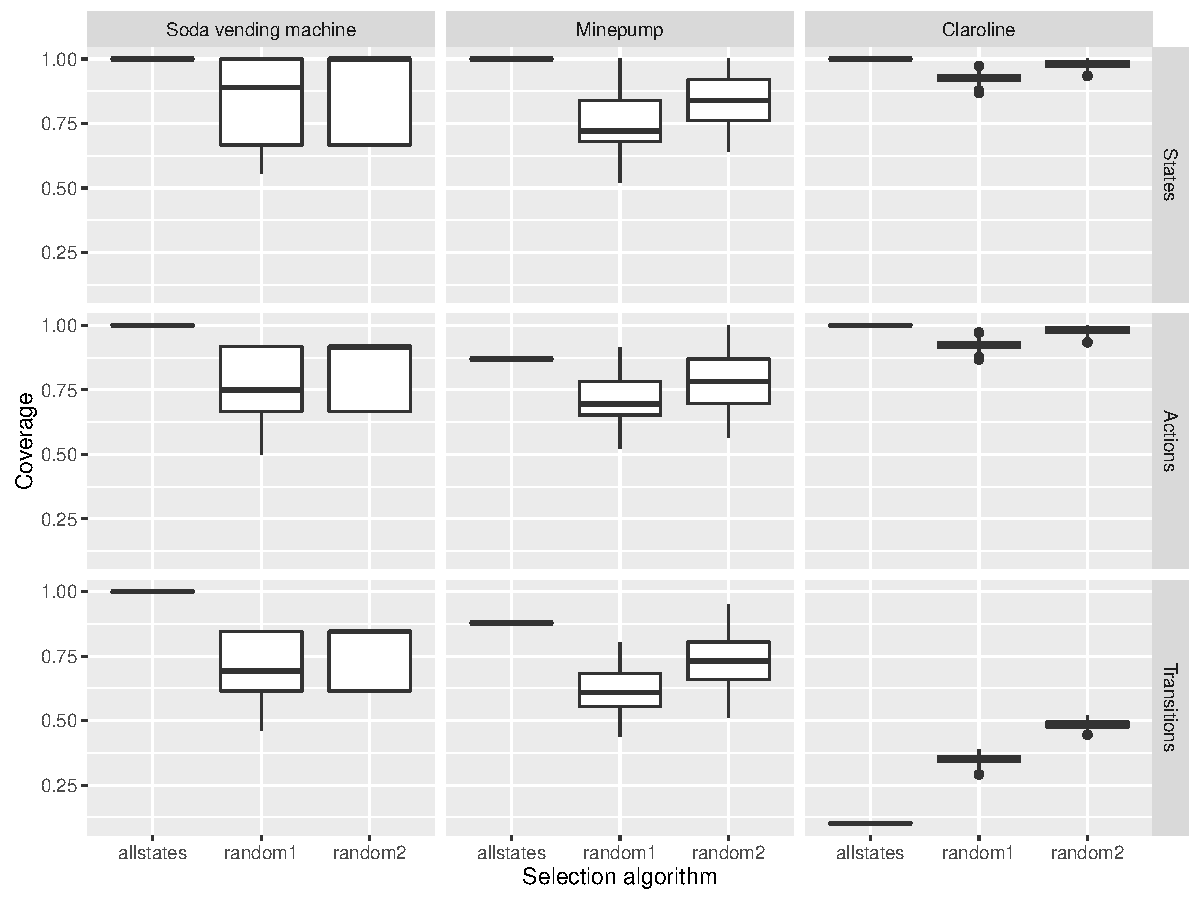
\includegraphics[width=\textwidth]{allstates-coverage}
	\caption{Structural coverages of the \textit{allstates}, \textit{random1}, and \textit{random2} test suites}
	\label{fig:allstatescoverage}
\end{figure}

Figure \ref{fig:allstatescoverage} presents the states, actions, and transitions coverage of the different test suites.  By construction, abstract test suites selected using our all-states algorithm (\textit{allstates} in Figure \ref{fig:allstatescoverage}) covers all the states for the three FTSs. On average, the random algorithm does not perform well to cover all the states of the different models.
On the contrary, the random algorithm performs better at covering transition on the largest model (Claroline): an average of 48.45\% for the 200 randomly selected test suites (\textit{random2}) against 10.17\% for the all-states selection algorithm.

%----------------------
\subsection{Discussion}
%----------------------

We investigated the difference between the \textit{allstates} and \textit{random(1,2)} transitions coverage for the Claroline model  and found that the all-states test suite contains only short test cases (2 actions). 
This is due to our heuristic. Since it prefers states that have a path to uncovered states, the initial state has the highest score in the Claroline model (because nearly all the states in the models have transitions coming from and going to the initial state, due to the web nature of the application). Changing the heuristic to avoid direct return to the initial state may improve the results for this kind of models (where each state is strongly connected to the initial state) but may increase the complexity of the algorithm and select inadequate abstract test cases for other kinds of models. 

These results are in line with the fact that all-states coverage criterion is poor to cover transitions in single systems \cite{Utting2007}, we assume that this is also the case for FTSs. Of courses an all-transitions algorithm would have given much better results (and all-states coverage). However our preliminary evaluation of such an algorithm resulted in huge scalability problems for the Claroline case study; after more than 3 days of selection and a text file describing the test suite of more 250 GB, our systems ran out  of memory (and also of hard drive space!).  Exhaustive computation of all-transitions for moderate size FTS is therefore not an option in most cases.    

Finally, we observe that the test suite selected to cover all-states in the Claroline FTS also covers all the actions. This is due to the nature of the model, since each state represents a page and each action represents a link followed from a page (\ie a state in the FTS) to another page (\ie another state), there are as many actions as there are states. Each action is thus covered. This is not always the case, \eg the soda vending machine in Figure \ref{fig:allstatescoverage}.

%--------------------------------
\subsection{Threats to validity}
%--------------------------------

\paragraph{Internal validity:}
%----------------------------

The all-states selection algorithm has been simplified to reduce the number of SAT calls which are very costly. This simplification gives good results on our largest model (Claroline) due to the few constraints on the FTS. On other models with more constraints on the different transitions, this simplification may give poor results since it can potentially select a lot of invalid test cases. We intend to compare the actual implementation which uses a SAT solver with binary decision diagrams (BDDs) which have performed better when processing FTSs \cite{Classen2011}.

The random selection of a test suite does not check whether there are duplicates abstract test cases or not. Since the size of the test suites considered for \textit{random2} test suites is larger than the size of the all-states covering test suite, this thread is limited. To avoid this, one may implement a filter to check that newly selected test suites are not duplicated.

\paragraph{Construct validity:}
%----------------------------

The Claroline FTS and its FM contain few constraints ending in a SPL with lots of products. We believe this is a typical characteristic of web applications which are a particular class of system. This has influenced the implementation of the random algorithm in order to minimize the number of SAT calls (which are costly in CPU time). It has also influenced the heuristic during the selection of the test suite covering all-states and gives very short test cases in regard to the size of the system. We plan to apply our algorithms on large industrial systems with more constrained FM and FTSs in order to validate our conclusions.

\paragraph{External validity:}
%----------------------------

To avoid too many SAT calls, we verify that an abstract test case is executable \textit{a posteriori} by calling the SAT solver once with the conjunction of the FM (represented as a boolean formula) and the feature expression of the transitions of the test case. We repeat the building of an abstract test case while it is not executable. Since the largest FTS model we considered does not have a lot of behaviours exclusive to subsets of the product line, this implementation of the random algorithm works fast. This may be not the case for other models with a lot of constrained behaviour.

As discussed by Inozemtseva et al. \cite{Inozemtseva2014}, a test suite with a good coverage does not guarantee the effectiveness of this test suite. However, in a first attempt to compare our selection algorithms, coverage seems to be a reasonable metric.


%%%%%%%%%%%%%%%%%%%%%%%%%%%%%%%%%%%%%%%%%%%
\section{Dissimilarity selection criteria}
%%%%%%%%%%%%%%%%%%%%%%%%%%%%%%%%%%%%%%%%%%%

\label{sec:experiment:dissimilarity}

We report hereafter on our evaluation of dissimilarity driven test suite selection \cite{Devroey2016}. In order to compare the different dissimilarity selections, we define the following research questions:
\begin{itemize}
\item \textbf{\textit{Dissimilarity relevance} (RQ.1) } How does the similarity-driven search based approach compare to all-actions and random test selection with respect to fault finding and product coverage?
\item \textbf{\textit{Distance impact} (RQ.2) } How does the choice of a given distance influences the results?
\end{itemize}


%--------------------
\subsection{Setup}
%--------------------

\label{sec:assessment:dissimilarity:setup}

We consider 4 models from different sources with different sizes as input to different test case selection processes. The four model are: the Soda vending machine (see section \ref{sec:casestudy:svm}), the Minepump (see section \ref{sec:casestudy:minepump}), the card payment terminal (see section \ref{sec:casestudy:cpterminal}), and Claroline (see section \ref{sec:casestudy:claroline}). In order to avoid bias using random selection, we run the evaluation 6 times for each model and each configuration of the algorithm (6 configurations overall) presented in this section.

\paragraph{Test suites selection:}
%---------------------------------

\begin{table}
	\centering
	\caption{Number of test cases and selection time of the all-actions test suites}
	\begin{small}
	\begin{tabular}{lrrrr}
		\hline
		\textbf{Model}	& \multicolumn{2}{c}{\textbf{Time ($d_{allactions}$)}} 	& \multicolumn{2}{c}{\textbf{Test cases ($k_{allactions}$)}}\\
						& $\overline{time}$ & $\sigma$		& $\overline{count}$	& $\sigma$	\\
		\hline 
		S. V. Mach.		& 1.03 sec. & 0.093	& 3.86	& 0.35	\\
		Minepump			& 1.18 sec. & 0.189	& 11.14	& 0.99	\\
		C. P. Term.		& 1.24 sec.	& 0.263	& 5.0	& 0.76	\\
		Claroline		& 3.42 sec.	& 1.814	& 52.86	& 2.95	\\
		\hline
	\end{tabular}
	\end{small}
	\label{tab:allactions:exec}
\end{table} 

For each model, we select a test suite which satisfies the \emph{all-actions} coverage criteria (\ie when executing all the test cases, all the actions of the FTS are executed at least once). We measure the selection time ($d_{allactions}$) and the number of test cases ($k_{allactions}$) and report in Table \ref{tab:allactions:exec}. 
%
The \emph{number of test cases} and the \emph{selection time} are used as input for the dissimilar test suite selections. To assess time impact ($d$  in Algorithm \ref{algo:diss}) on the results, we consider the following values: $1 \times d_{allactions}$, $2 \times d_{allactions}$, $10 \times d_{allactions}$, and $100 \times d_{allactions}$ to parametrize the time during which the evolutionary algorithm runs. 
%
We configure the algorithm using different \emph{distances} to compute the fitness function: the Jaccard index for product dissimilarity; and the Hamming distance, Jaccard index, dice and anti-dice, and Levenshtein distances for actions dissimilarity. We combine product dissimilarity and actions dissimilarity using the multiplication and average operator ($\otimes$), and also consider action dissimilarity alone. For each configuration, we run the algorithm  using local and global distances for the sort.
%
For each model, A \emph{random} suite of $k_{allactions}$ test cases is also selected (see Algorithm \ref{algo:random}). In total, we selected 122 test suites for each model.


\paragraph{Fault injection and test suites execution:}
%------------------------------------------------------

\begin{table}
	\centering
	\caption{Number of faulty states, transitions, and actions seeded in the models}
	\begin{small}
	\begin{tabular}{lrrrrrr}
		\hline
		\textbf{Model}	& \multicolumn{2}{c}{\textbf{Faulty States}}	& \multicolumn{2}{c}{\textbf{Faulty Transitions}} & \multicolumn{2}{c}{\textbf{Faulty Actions}} \\
						& \textit{$\overline{faults}$} & \textit{$\sigma$}	& \textit{$\overline{faults}$} & \textit{$\sigma$}	& \textit{$\overline{faults}$} & \textit{$\sigma$}\\
		\hline 
		S. V. Mach.		& 4.6	& 0.8	& 5.9	& 1.0	& 5.7	& 1.0	\\
		Minepump			& 12.4	& 1.4	& 19.3	& 1.7	& 9.6	& 1.5	\\
		C. P. Term.		& 5.3	& 0.9	& 7.9	& 1.1	& 6.8	& 1.1	\\
		Claroline		& 52.1	& 2.9	& 896.8	& 13.3	& 32.3	& 2.9	\\
		\hline
	\end{tabular}
	\end{small}
	\label{tab:avg:faults}
\end{table}

Fault seeding is a popular technique to assess and compare test suites coverage \cite{Andrews2005,Andrews2006,Mathur2008}. The idea is to inject faults in SUT and measure the number of faults detected by the test suite. 
%In a SPL context, fault injection (using mutation testing) has been applied to feature models by Henard et al. \cite{Henard2013b}. 
%We did not consider fault injection in the FM, in place 
In this evaluation, we choose to artificially inject faults into the FTS by tagging state, transitions and actions as faulty. We randomly select states, transitions, and actions to assume them as faulty (\ie containing a fault), if a state/transition/action is selected more than once, it is only counted as 1 during the fault detection. We then execute the test suites on the FTS and consider that a fault is revealed as soon as the faulty states is reached, the faulty transitions are fired, and the faulty actions are executed.
Using information coming from previous versions of the system (\ie from a bug tracker), this would allow one to tag elements of the model that are more likely to contain faults.
In our case, we do not have access to such information and use a random selection with an upper bound of 66\% of faults of the states, actions, and transitions of the FTS. This gives a measure is close to states, actions, and transitions coverage but still allows to finely compare the different approaches. Table \ref{tab:avg:faults} presents the average number of faults seeded in the different models during the evaluation.

%--------------------
\subsection{Results}
%--------------------

\begin{figure}
	\centering
	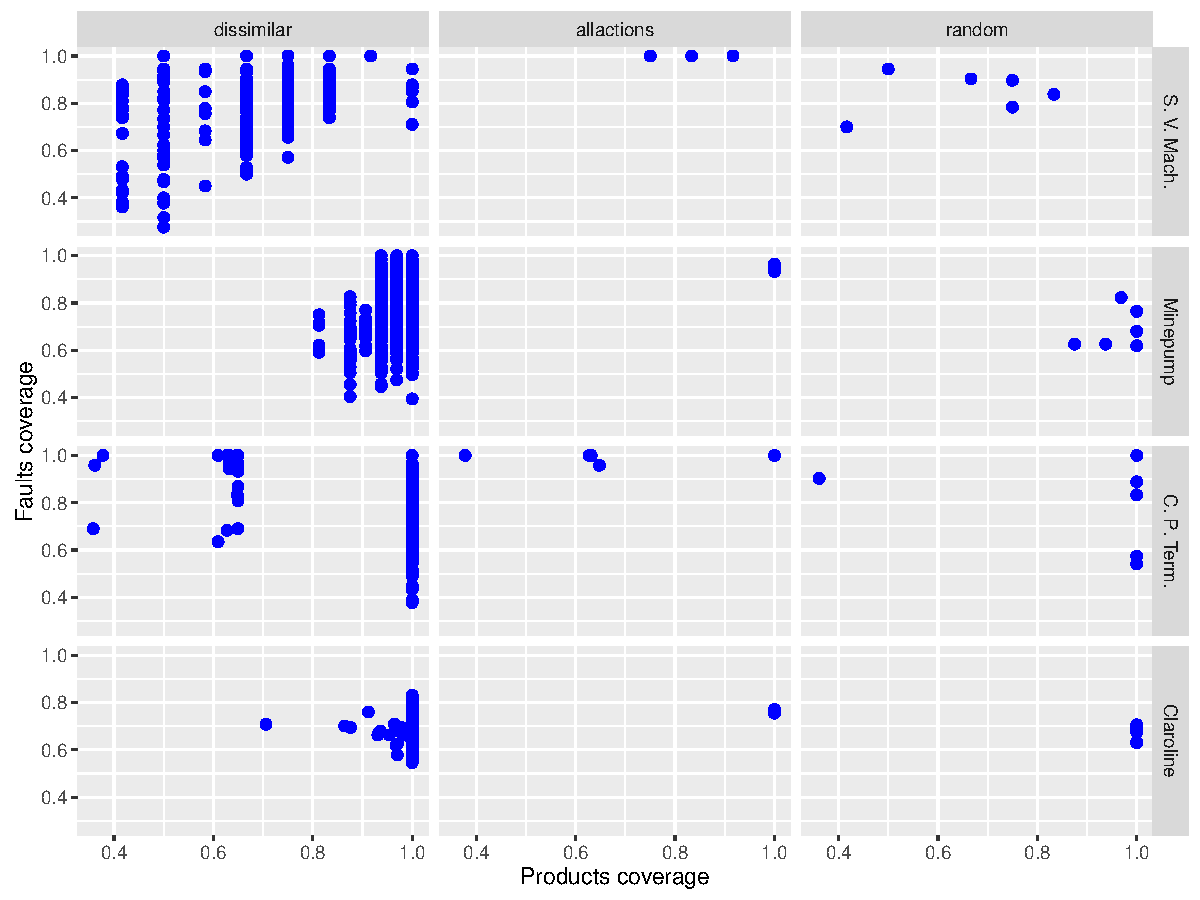
\includegraphics[width=0.98\textwidth]{diss-coverages}
	\caption{Faults coverage of the all-actions, random, and dissimilar test suites}
	\label{fig:assessment:faultscoverage}
\end{figure}

Figure \ref{fig:assessment:faultscoverage} presents the coverage distribution of the different test suites selected using dissimilarity, all-actions coverage, and random algorithm. The x-axis is the percentage of products covered by the test suite: for a suite $s$ and a feature model $d$, it corresponds to $\frac{\#prod(d, s)}{\# [\![d]\!]}$. The y-axis is the percentage of faults (states, transitions, or actions) discovered when executing the test suite.

To characterize the test suites (\ie, the solution space of our bi-objective selection), we compute a \emph{reference front}, by taking the Pareto front of \emph{all} the points in Figure \ref{fig:assessment:faultscoverage}. This reference front contains all the sets of test cases maximising the fault and products coverages (\ie, the best solutions). We give hereafter for each model a podium with the 3 (or more if they have the same frequency) optimal configurations of the dissimilarity-based selection providing solutions that are on the reference front:
\begin{itemize}
\item \textbf{Soda vending machine} (47 optimal solutions)
	\begin{itemize}
	\item Hamming avg., global, $t=10$ ($freq. = 0.056$)
	\item Hamming avg., global, $t=1$ ($freq. = 0.056$)
	\item Hamming avg., global, $t=2$ ($freq. = 0.056$)
	\item Hamming avg., global, $t=100$ ($freq. = 0.056$)
	\end{itemize}
\item \textbf{Minepump} (6 optimal solutions)
	\begin{itemize}
	\item Jaccard sing., global, $t=2$ ($freq. = 0.222$)
	\item Jaccard avg., global, $t=10$ ($freq. = 0.222$)
	\item Antidice sing., global, $t=1$ ($freq. = 0.222$)
	\end{itemize}
\item \textbf{Card payment terminal} (64 optimal solutions)
	\begin{itemize}
	\item Levenshtein sing., global, $t=2$ ($freq. = 0.029$)
	\item Antidice sing., global, $t=10$ ($freq. = 0.029$)
	\item Levenshtein sing., global, $t=2$ ($freq. = 0.029$)
	\item Antidice mul., global, $t=2$ ($freq. = 0.029$)
	\item Antidice avg., global, $t=2$ ($freq. = 0.029$)
	\end{itemize}
\item \textbf{Claroline} (1 optimal solution)
	\begin{itemize}
	\item Hamming sing., global, $t=100$ ($freq. = 1.0$)
	\end{itemize}
\end{itemize}


\begin{table}
	\centering
	\caption{Hypervolumes values for the Claroline case-study}
	

%\begin{tabular}{l r c c c c c c  c c c  c c c  c c c }
%\hline
%% Titles
%\multicolumn{2}{r}{ } & \multicolumn{15}{c}{\textbf{Actions dissimilarity distance}} \\
%% Selection criteria
%\multicolumn{2}{r}{ } & \multicolumn{3}{c}{\textbf{Hamming}} & \multicolumn{3}{c}{\textbf{Jaccard}} & \multicolumn{3}{c}{\textbf{Dice}} & \multicolumn{3}{c}{\textbf{Antidice}} &  \multicolumn{3}{c}{\textbf{Levenshtein}}\\
%% Mul and Avg
%& \textit{t} & \textit{Avg.} & \textit{Mul.} & \textit{Sing.} & \textit{Avg.} & \textit{Mul.} & \textit{Sing.} & \textit{Avg.} & \textit{Mul.} & \textit{Sing.} & \textit{Avg.} & \textit{Mul.} &  \textit{Sing.} & \textit{Avg.} & \textit{Mul.} & \textit{Sing.} \\ 
%\hline
%% Values
% & \textit{1} & 0.688 & 0.662 & 0.690 & 0.673 & 0.705 & 0.690 & 0.693 & 0.709 & 0.690 & 0.711 & 0.692 & 0.668 & 0.691 & 0.722 & 0.691 \\
%\textbf{Loc.} & \textit{2} & 0.674 & 0.699 & 0.705 & 0.679 & 0.673 & 0.684 & 0.667 & 0.689 & 0.670 & 0.688 & 0.690 & 0.659 & 0.666 & 0.662 & 0.677\\
%\textbf{sort} & \textit{10} & 0.702 & 0.681 & 0.661 & 0.721 & 0.685 & 0.700 & 0.720 & 0.669 & 0.679 & 0.667 & 0.674 & 0.651 & 0.691 & 0.681 & 0.696 \\
% & \textit{100} & 0.667 & 0.693 & 0.672 & 0.672 & 0.720 & 0.713 & 0.691 & 0.703 & 0.678 & 0.696 & 0.685 & 0.655 & 0.655 & 0.678 & 0.687 \\
% & \textit{1} & 0.736 & 0.710 & 0.724 & 0.694 & 0.697 & 0.727 & 0.695 & 0.683 & 0.710 & 0.666 & 0.672 & 0.699 & 0.684 & 0.693 & 0.717 \\
%\textbf{Glob.} & \textit{2} & 0.711 & 0.708 & 0.755 & 0.722 & 0.718 & 0.715 & 0.723 & 0.670 & 0.729 & 0.677 & 0.705 & 0.728 & 0.708 & 0.687 & 0.733 \\
%\textbf{sort} & \textit{10} & 0.740 & 0.733 & 0.804 & 0.723 & 0.696 & 0.730 & 0.690 & 0.683 & 0.738 & 0.701 & 0.692 & 0.746 & 0.701 & 0.714 & 0.771 \\
% & \textit{100} & 0.794 & 0.800 & 0.831 & 0.747 & 0.729 & 0.756 & 0.750 & 0.714 & 0.755 & 0.747 & 0.740 & 0.758 & 0.747 & 0.730 & 0.781 \\	
%\hline
%\multicolumn{2}{l}{\textbf{All-act. crit.}}	& \multicolumn{15}{l}{0.771} \\
%\multicolumn{2}{l}{\textbf{Rand. crit.}}	& \multicolumn{15}{l}{0.706}  \\
%\end{tabular}


\begin{small}
\begin{tabularx}{0.98\textwidth}{X r  c c c  c c c  c c c}
%\begin{tabular}{l r  c c c  c c c  c c c}
\hline
% Selection criteria
\multicolumn{2}{r}{} & \multicolumn{3}{c}{\textbf{Hamming}} & \multicolumn{3}{c}{\textbf{Jaccard}} & \multicolumn{3}{c}{\textbf{Dice}} \\
% Mul and Avg
& \textit{t} & \textit{Avg.} & \textit{Mul.} & \textit{Sing.} & \textit{Avg.} & \textit{Mul.} & \textit{Sing.} & \textit{Avg.} & \textit{Mul.} & \textit{Sing.} \\ 
\hline
% Values
 				& \textit{1} & 0.688 & 0.662 & 0.690 & 0.673 & 0.705 & 0.690 & 0.693 & 0.709 & 0.690 \\
\textbf{Loc.}	& \textit{2} & 0.674 & 0.699 & 0.705 & 0.679 & 0.673 & 0.684 & 0.667 & 0.689 & 0.670 \\
\textbf{sort}	& \textit{10} & 0.702 & 0.681 & 0.661 & 0.721 & 0.685 & 0.700 & 0.720 & 0.669 & 0.679 \\
				& \textit{100} & 0.667 & 0.693 & 0.672 & 0.672 & 0.720 & 0.713 & 0.691 & 0.703 & 0.678 \\
 				& \textit{1} & 0.736 & 0.710 & 0.724 & 0.694 & 0.697 & 0.727 & 0.695 & 0.683 & 0.710 \\
\textbf{Glob.}	& \textit{2} & 0.711 & 0.708 & 0.755 & 0.722 & 0.718 & 0.715 & 0.723 & 0.670 & 0.729 \\
\textbf{sort}	& \textit{10} & 0.740 & 0.733 & 0.804 & 0.723 & 0.696 & 0.730 & 0.690 & 0.683 & 0.738 \\
				& \textit{100} & 0.794 & 0.800 & 0.831 & 0.747 & 0.729 & 0.756 & 0.750 & 0.714 & 0.755 \\
\hline
\end{tabularx}
%\end{tabular}

\begin{tabular}{l r  c c c  c c c}
 % Selection criteria
\multicolumn{2}{r}{ } & \multicolumn{3}{c}{\textbf{Antidice}} &  \multicolumn{3}{c}{\textbf{Levenshtein}}  \\
% Mul and Avg
& \textit{t} & \textit{Avg.} & \textit{Mul.} & \textit{Sing.} & \textit{Avg.} & \textit{Mul.} & \textit{Sing.}\\	
\hline
% Values
              & \textit{1} 	& 0.711 & 0.692 & 0.668 & 0.691 & 0.722 & 0.691 \\
\textbf{Loc.} & \textit{2} 	& 0.688 & 0.690 & 0.659 & 0.666 & 0.662 & 0.677 \\
\textbf{sort} & \textit{10} 	& 0.667 & 0.674 & 0.651 & 0.691 & 0.681 & 0.696 \\
              & \textit{100}	& 0.696 & 0.685 & 0.655 & 0.655 & 0.678 & 0.687 \\
              & \textit{1} 	& 0.666 & 0.672 & 0.699 & 0.684 & 0.693 & 0.717 \\
\textbf{Glob.}& \textit{2} 	& 0.677 & 0.705 & 0.728 & 0.708 & 0.687 & 0.733 \\
\textbf{sort} & \textit{10} 	& 0.701 & 0.692 & 0.746 & 0.701 & 0.714 & 0.771 \\
              & \textit{100}	&  0.747 & 0.740 & 0.758 & 0.747 & 0.730 & 0.781  \\
\hline
\end{tabular}

\begin{tabular}{c c}
\textbf{All-action}	& \textbf{Random}	\\
\hline
 0.771 & 0.706 \\
\hline
\end{tabular}

\end{small}

	\label{tab:claroline:hypervolumes}
\end{table}

Finally, Table \ref{tab:claroline:hypervolumes} presents hypervolume for the Claroline model for the different test suites. The hypervolume corresponds, for a test suite $s$, to the volume of the solution space dominated by $s$ \cite{Brockhoff2008,Henard2015}. A high value of hypervolume correspond to a set of test cases with a better fault and product coverage.
Rows and columns show the parameters values used for dissimilarity-based selection: the top rows indicate the actions dissimilarity distance ($diss_a$) and the operator ($\otimes$) used to combine it with the product distance ($diss_p$) or if the actions dissimilarity distance is used alone, \ie  in a single-objective configuration of the algorithm (denoted by \textit{Sing.} in the table); the leftmost columns indicate which sorting method is used (global or local) and the time considered for the algorithm ($1 \times d_{allactions}$, $2 \times d_{allactions}$, $10 \times d_{allactions}$, or $100 \times d_{allactions}$). 

The raw results for the 6 executions of the different test case selection algorithms and their fault finding evaluation may be downloaded at \url{http://projects.info.unamur.be/vibes}


%----------------------
\subsection{Discussion}
%----------------------

\paragraph{Dissimilarity relevance:} 
%-----------------------------------

Regarding \emph{RQ.1}, dissimilarity-based approaches are always able to obtain the optimal results in terms of fault finding ability and coverage.  On the three small models, these results are sometimes matched by the all-actions and random approaches (Figure \ref{fig:assessment:faultscoverage}).  However, the latter appear less frequently: neither random  nor all-actions are on the podium of optimal solutions in terms of frequency. Additionally on the Claroline case study, the only optimal solution found is a search-based one. We therefore confirm the good results of similarity-driven testing for single product testing \cite{Mondal2015} and product selection at the feature model level \cite{Henard2014a} for behavioural test case selection in an SPL context. 

The most important finding is that being fully bi-objective is not necessarily an advantage: on the 13 approaches present in the frequency podiums, only 6 are bi-objective. Additionally, a single objective approach dominates alone the Claroline case. This may be due to the nature of the case study, which is not heavily constrained: it is easy to obtain by chance dissimilar products. All-actions performance may benefit of this situation as well. Time may  be involved in the explanation: for a given amount of time, a bi-objective configuration will necessarily iterate less than a single-objective one.  

When bi-objective is optimal, the average (\textit{Avg.}) composition operator gives the best results as only one \textit{Mul.} approach appears on our podiums. Time given to the search-based algorithm has an (expected)  influence on the quality of the results.  This is apparent on the Claroline case where the best hypervolumes  are obtained by approaches that are given $t=100$.       

\paragraph{Distance impact:}
%---------------------------

If we consider all the podiums, Hamming and Jaccard-based distances (Dice, Antidice, Jaccard)  clearly win over Levenshtein.  This may seem surprising since Levenshtein  is the only one that is sequence-based taking into account the order of the actions.  Levenshtein is more computationally expensive than Hamming and Jaccard-based distances, implying less iterations of the algorithm for a given amount of time.  When employed alone (single-objective) on actions, it appears to be the second most performing distance on the Claroline case.       


%--------------------------------
\subsection{Threats to validity} 
%--------------------------------

%\paragraph{Construct validity:}
%---------------------------

To keep the comparison fair between the different test suite selection algorithms, we use the same number of test cases and duration time of the all-actions test suite selection to parametrize random and dissimilar test suites selections. As the dissimilar test suite selection is based on a (1+1) evolutionary algorithm \cite{Droste2002}, it is very sensitive to the maximal execution time ($d$). The all-actions test suite selection may be very fast (for the soda vending machine for instance). In order to assess the time influence in the quality of selection for the evolutionary approach, we chose to repeat the test case selection with different $d$ values.

We chose to use a (1+1) evolutionary algorithm \cite{Droste2002} to maximize the dissimilarity of the selected test suite. This algorithm is simple and to parametrize, and it showed good results to select products to test \cite{Henard2014a}. Many other algorithms, like adaptive random testing \cite{Chen2010}, used to select dissimilar test cases exist \cite{Hemmati2013}. A comparison between those different algorithms is left for future work.

The complete process described in Section \ref{sec:assessment:dissimilarity:setup} has been repeated 6 times for each model on a Ubuntu Linux machine (Linux version 3.13.0-65-generic, Ubuntu 4.8.2-19ubuntu1) with an Intel Core i3 (3.10GHz) processor and 4GB of memory. The complete experiment took approximately 4 days.

%\paragraph{External validity:}
%%---------------------------
%
%We cannot guarantee that our models are representative of real behavioural models. The soda vending machine, Minepump, and card payment terminal models are small with few states and transitions. The Claroline model is a larger model reverse engineered from a running web application, this gave us a model with a very flexible navigation (\ie a large number of transitions) between states (representing pages) with very few exclusive constraints (\ie feature expressions) on the transitions. This has the side effect to allow many products to execute a large part of the FTS with few behaviours limited to a small subset of the SPL. 
%However, the diversity of the models sources as well as the diversity of considered systems gives us good confidence in the possibilities of this approach. In our future work, we will apply our approach on other kinds of systems from various domains where the transitions from state to state are more constrained and/or where the SPL has specific behaviour exercised only by a small subset of the possible products.



%%%%%%%%%%%%%%%%%%%%%%%%%%%%%%%%%%%%%%%%%%%%%%%%%%%%%%%%%%%%%%%%%%%%%%%%%
\section{Behavioural coverage of products sampling techniques}
%%%%%%%%%%%%%%%%%%%%%%%%%%%%%%%%%%%%%%%%%%%%%%%%%%%%%%%%%%%%%%%%%%%%%%%%%

\label{sec:experiment:beahviouralcoverage}

Products selection approaches solely based on the feature model, such as \textit{t}-wise testing, have gained momentum as they are able to scale to large SPLs. However, these methods are agnostic with respect to behaviour: the sampled products have no reason to satisfy any given structural behavioural criterion. In this section, we report on our investigation \cite{Devroey2015b} on the behavioural coverage of two products selection approaches: \textit{t}-wise selection and dissimilarity-based selection. To do so, we describe hereafter our \emph{initial assessment} in order to answer the following research question:
%
\begin{itemize}
\item  \textbf{\textit{Behavioural coverage} } Which behavioural coverage do dissimilarity and \textit{t}-wise sampling achieve?
\end{itemize} 
%
To address this question, we use four SPLs: each is modelled by a FTS and its related feature model. We then apply \textit{t}-wise and dissimilarity techniques to sample a set of products. By projecting the FTS for each sampled product, we get a 
labelled transition system from which it is possible to compute the coverage of the FTS representing the whole SPL.

Preliminary results indicate that full coverage of states, transitions and actions can indeed be achieved with few products (no more than 3) and that 3-wise sampling worked best in these cases. Dissimilarity works better than \textit{t}-wise for $t=\{1,2\}$, although a detailed comparison is beyond the scope of this assessment. All these samplings obtain full coverage with more products than needed, indicating an interesting potential for mixing products coverage and behavioural coverage rather than systematically considering them in isolation.

%--------------------
\subsection{Setup}
%--------------------

This initial assessment is performed on the soda vending machine, the Minepump, the Sferion\texttrademark landing symbology function, and Claroline.  Regarding t-wise sampling, we elicit the SPLCAT tool \cite{Johansen2012} for its performance \cite{Henard2014} and PLEDGE \cite{Henard2014a} for similarity testing. Behaviour of the different models is represented using FTSs. To measure the behavioural coverage we use state, transition and action coverage for each product selected using the different structural criteria. 

To perform our assessment, we carry out the following steps for each model and each tool (SPLCAT and PLEDGE):
\begin{enumerate}
\item select a set of products from the feature model using each tool;
\item project the FTS on each product, to get the behavioural model (\ie, the LTS) corresponding to this product (we use the projection operator defined by Classen et al. \cite{Classen2013b}): it creates a new labelled transition system by removing all transitions that may not be executed by the product, unreachable states, and unused actions (feature expressions are dropped during the process);
\item for each product, compute the coverage of its behavioural model: divide the number of states, transitions, and actions in the projection by the number of states, transitions, and actions in the FTS. The cumulated coverage is calculated by dividing the number of different states, transitions, and actions in the projections by the number of different states, transitions, and actions in the FTS. The states, transitions, and actions appearing more than once are thus counted only once.
\end{enumerate}

\begin{table}
\centering
\caption{SPLCAT and PLEDGE parameters}
\label{tab:behavcov:toolsparams}
\begin{small}
\begin{tabular}{lcccc}
\hline
\textbf{Model}	& \textbf{SPLCAT} 	& \multicolumn{2}{c}{\textbf{PLEDGE}}& \textbf{Config.}  \\
				& \textit{t}	& \textit{x}		& \textit{d}		&  \\
\hline
Soda V. M.		& 1				& 3			& 30 sec.		& 3				\\
				& 2				& 6			& 30 sec.		& 6				\\
				& 3				& 14			& 30 sec.		& 14				\\
Minepump			& 1				& 2			& 30 sec.		& 2				\\
				& 2				& 7			& 30 sec.		& 7				\\
				& 3				& 13			& 30 sec.		& 13				\\
Aero UC5			& 1				& 2			& 60 sec.		& 2				\\
				& 2				& 8			& 60 sec.		& 8				\\
				& 3				& 15			& 60 sec.		& 15				\\
Claroline		& 1				& 6			& 60 sec.		& 6				\\
				& 2				& 21			& 60 sec.		& 21				\\
				& 3				& 71			& 60 sec.		& 71				\\
\hline
\end{tabular}
\end{small}
\end{table}


The feature model of each case study is used as input to the SPLCAT and PLEDGE tools to select sets of products. The SPLCAT tool can sample, for a given model and a given $t$ between 1 and 3, a set of valid products satisfying the 1-wise, 2-wise, or 3-wise  coverage criteria over the feature model. The PLEDGE tool can sample, for a given feature model, a given number of products $x$, and a certain time $d$, a set containing $x$ products, using an evolutionary algorithm maximising the dissimilarity (in terms of features selected) amongst products in this set. We use as $x$ the number of products sampled by SPLCAT for each model. The $d$ parameter has the default value $60$ seconds, except for smaller models where it had, after few trials, to be reduced to $30$ seconds to avoid memory errors during execution. Table \ref{tab:behavcov:toolsparams} presents the different parameters used for each model and the number of sampled products. We ran the tools on a Ubuntu Linux machine with an Intel Core i3 (3.10GHz) processor and 4GB of memory.

%--------------------
\subsection{Results}
%--------------------

\begin{figure}
	\centering
	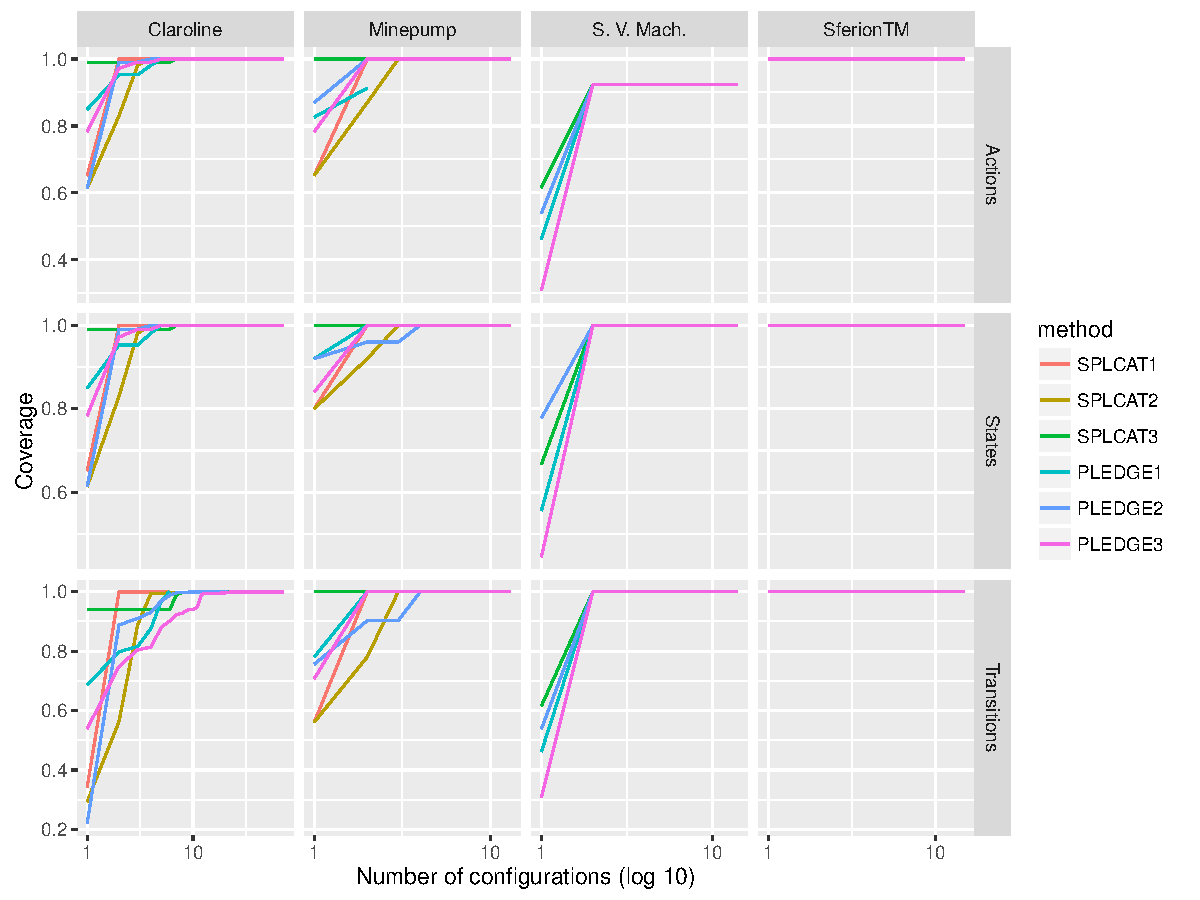
\includegraphics[width=1\textwidth]{configurations-coverage}
	\caption{Behavioural coverage of products selected using SPLCAT and PLEDGE tools}
	\label{fig:behavcov:results}
\end{figure}

Figure \ref{fig:behavcov:results} presents the accumulate behavioural coverage in terms of actions, states, and transitions of the products selected using SPLCAT and PLEDGE. 
%
Results for the soda vending machine exhibit the same tendencies as those of the Minepump. The Sferion\texttrademark landing symbology function has a coverage of $100\%$ for states, transitions, and actions for every product sampled using SPLCAT and PLEDGE, because its FTS has only 4 transitions specific to 2 different features, 2 transitions for each feature, present in each product.
%
Although the number of selected products is higher (as shown in Table \ref{tab:behavcov:toolsparams}), in general, the cumulated coverage value did not increase further after 7 products for states and actions coverage and 14 products for transitions coverage.

%----------------------
\subsection{Discussion}
%----------------------

Regarding our research question, for the considered case studies and settings, we rapidly obtain a complete coverage: relatively few products are needed to fully cover states, transitions, and actions for the two tools reported here. This is to be expected for our small case studies, but on a larger model (Claroline), this tendency tends to be confirmed. Of course, this assessment need to be replicated on a larger sample of behavioural models, but this seems encouraging for the usage of structural coverage criteria at the feature model level beyond the scope of detecting behavioural feature interactions \cite{Cichos2011}. 

On the small feature models, exact $t$-wise coverage (SPLCAT) yields better coverage on all our behavioural criteria for $t=3$. This further indicates that higher values than the usual 2-wise are relevant \cite{Steffens2012} and therefore should be used when the number of products is reasonable. PLEDGE tends to outperform  SPLCAT on 1-wise (each feature is covered at least once) and 2-wise with a smaller number of products. Since for a given execution time, a smaller number of products means more time to  evolve the population (set of products) and less time spent computing distances amongst them, maybe the poor performance of PLEDGE for $t=3$, the largest number of products, can be explained in such a way. We also use the local maximum distance  (called \textit{greedy} in the tool), which is outperformed in terms of coverage by the global maximum distance (called \textit{NearOptimal} in the tool) \cite{Henard2014}. It also  seems that some of the memory errors we run into (related to thread creation) can be accounted by this default choice of the algorithm. Indeed, threads are associated to evolutions of the population and local distance algorithm is fast: we therefore have a thread explosion problem on these small feature models. Therefore, additional settings and trade-offs need to be investigated to be able to compare the tools. Detailed tool comparison in this context is beyond the scope of our research question and is therefore left for future work.

Finally, for both approaches, this initial assessment shows that there is also a need for prioritisation and optimal behavioural coverage. For example, amongst the 71 products selected by SPLCAT ($t=3$), only one is sufficient to cover all states on both the Minepump and Claroline models. This product can be found directly using the all-states coverage test case selection algorithm and the p-coverage upper bound property. If dissimilarity and \textit{t}-wise coverage are shown to consistently sample products that achieve good behavioural coverage, as this assessment suggests, then they can be used as first filters on very large feature models (assuming an intractable FTS for a test case selection algorithm) to prune the FTS and then perform a behavioural coverage driven test case selection. Prioritisation may be initiated at the FTS level and combined with behavioural/structural criteria. There is no such one-criteria-fits-all approach in this endeavour: an all-states criterion may poorly cover transitions (\eg on the Claroline case).  Exploring synergies between these criteria, both at the structural and behavioural models, therefore seems the best option.   


%--------------------------------
\subsection{Threats to validity}
%--------------------------------

%\paragraph{Construct validity:}
%----------------------------

The PLEDGE input parameters are arbitrarily chosen. To keep a fair comparison between the results of the PLEDGE and SPLCAT tools, we keep the same number of products $x$ as sampled by SPLCAT. Estimating the time $d$, however is more tricky. In their comparison, Henard \etal \cite{Henard2014} use the same sampling time as SPLCAT. Unfortunately in our case, some \textit{t}-wise computations take less than 1 second in SPLCAT and PLEDGE does not allow to enter such values. Thus we initially went for the default values provided by the tool. As mentioned above, playing with a wider range of parameter values and with different similarity algorithms will mitigate this threat.

FTS models relate variability to behaviour using feature expressions on transitions, other modelling languages may relate variability to behaviour in other ways (\eg associate variability to states instead of transitions), which will give different results for the state, transitions and actions coverage. FTS is a basic formalism to which we can easily transform other modelling languages and mappings. Thus, we can investigate the influence of the mapping between features and behavioural models.    

%\paragraph{External validity:}
%%----------------------------
%
%We cannot guarantee that our 4 models are representative of real SPLs. We mixed sources and domains to mitigate this threat. 
%The small number of features in the considered feature model does not allow us to generalize our results for large product lines. To the best of our knowledge, there exists no feature model with both a large number of features and an associated behavioural model accessible for research and experimentation.


%%%%%%%%%%%%%%%%%%%%%%%%%%%%%%%%%%%%%%%%%%%%%%%%%%%%%%%%%%%%%%%%%%%%%%%%%
\section{Usage selection and prioritization criteria}
%%%%%%%%%%%%%%%%%%%%%%%%%%%%%%%%%%%%%%%%%%%%%%%%%%%%%%%%%%%%%%%%%%%%%%%%%

\label{sec:experiment:usage}

In this section,  we report on the \emph{feasibility} of using family-based test selection \cite{Devroey2014,Devroey2015a} by applying it on two systems: the first one is Claroline (see section \ref{sec:casestudy:claroline}), and the second one is the landing symbology function, part of Sferion\texttrademark (see section \ref{sec:casestudy:sferion}). Validation of the product-based test selection has been done by Samih \etal \cite{Samih2014}.
%
We assess the feasibility of our approach using the following research questions:
\begin{itemize}
\item \textbf{\textit{FTS pruning} (RQ.1) } What are the reductions gains (model pruning) achieved by applying statistical  prioritization?    
\item \textbf{\textit{Modelling} (RQ.2) } What is the modelling effort induced by our approach and what are the consequences of modelling choices?
\item \textbf{\textit{Scalability} (RQ.3) } How does prioritization scale to increasing probability ranges and what are the implications for testing?  
\end{itemize}

It is difficult to provide precise thresholds for these criteria. Testing should fit a given budget, which is a complex trade-off involving testing time, human and infrastructure resources, level of system coverage desired, \etc  Statistical approaches covered in this thesis are  flexible to meet such a tradeoff. We argue that fixing meaningful  thresholds values requires additional experience, especially in industrial settings where they both can be set and assessed. We therefore leave this issue for future work, giving both quantitative and qualitative information stemming from our experience applying our techniques on Claroline and Sferion\texttrademark.    

%-----------------------------------------------------------
\subsection{Claroline, an online course management system}
%-----------------------------------------------------------

\paragraph{Setup:}
%----------------

We derived the \gls{usage model}, from the same anonymized Apache webserver log as for Claroline FTS (see section \ref{sec:casestudy:claroline:fts}), using a classical bigram inference technique \cite{Ghezzi2014,Sampath2008,Sprenkle2013}: algorithm \ref{algo:bigram} has been adapted to produce a usage model giving algorithm \ref{algo:bigramusagemodel}. As previously, we consider resource names in the user sessions as states (lines \ref{algo:bigramusagemodel:line:sessioninit1} and \ref{algo:bigramusagemodel:line:addstate}) and add transitions between those names if they appear successively in the user sessions (lines \ref{algo:bigramusagemodel:line:sessioninit4} and \ref{algo:bigramusagemodel:line:addtransition}). To compute the probability of each transition, we count the number of occurrences of the transitions (lines \ref{algo:bigramusagemodel:line:sessioninit5}, \ref{algo:bigramusagemodel:line:incrementtrcount}, and \ref{algo:bigramusagemodel:line:incrementfinaltrcount}) and for each transition, we divide this count by the total number of occurrences having the same source state (lines \ref{algo:bigramusagemodel:line:probaloop} and \ref{algo:bigramusagemodel:line:probadef}).

\begin{algorithm}[t]
	\KwIn{$sessions$: the set of non empty user sessions}
	\KwOut{$um$: a usage model representing a navigational model for the given user sessions}
	\Begin{
		$S = \{ s_0 \}$; $Act = \emptyset$; $trans = \emptyset$; $\tau(s_0) = 1$\; \nllabel{algo:bigramusagemodel:line:init}
		\For{sess $\in$ sessions \nllabel{algo:bigramusagemodel:line:mainloop}}{
			$S.add(sess[0])$\; \nllabel{algo:bigramusagemodel:line:sessioninit1}
			$Act.add(req(sess[0]))$ \; \nllabel{algo:bigramusagemodel:line:sessioninit2}
			$tr = s_0 \xrightarrow{req(sess[0])} sess[0]$\; \nllabel{algo:bigramusagemodel:line:sessioninit3}
			$trans.add(tr)$\; \nllabel{algo:bigramusagemodel:line:sessioninit4}
			$count(tr) = count(tr) + 1$\; \nllabel{algo:bigramusagemodel:line:sessioninit5}
			\For{$i \in [1;sess.size[$ \nllabel{algo:bigramusagemodel:line:sessionloop}}{
				$S.add(sess[i])$\;  \nllabel{algo:bigramusagemodel:line:addstate}
				$Act.add(req(sess[i]))$\; \nllabel{algo:bigramusagemodel:line:addaction}
				$tr = sess[i-1] \xrightarrow{req(sess[i])} sess[i]$\; 
				$trans.add(tr)$\; \nllabel{algo:bigramusagemodel:line:addtransition}
				$count(tr) = count(tr) + 1$\; \nllabel{algo:bigramusagemodel:line:incrementtrcount}
	  		}
			$Act.add(req(s_0))$\; 
			$tr = sess[sess.size - 1] \xrightarrow{req(s_0)} s_0$\;
			$trans.add(tr)$\;	 \nllabel{algo:bigramusagemodel:line:addfinaltransition}
			$count(tr) = count(tr) + 1$\; \nllabel{algo:bigramusagemodel:line:incrementfinaltrcount}
	  	}
		\For{$(s_k \xrightarrow{\alpha_i} s_l) \in trans$ \nllabel{algo:bigramusagemodel:line:probaloop}}{
			$P(s_k \xrightarrow{\alpha_i} s_l) = \dfrac{count(s_k \xrightarrow{\alpha_i} s_l)}{\sum_{(s_k \xrightarrow{\alpha_j} s_m) \in trans} count(s_k \xrightarrow{\alpha_j} s_n)} $\; \nllabel{algo:bigramusagemodel:line:probadef}
		}
	  	$um = (S, Act, trans, P, \tau)$\; \nllabel{algo:bigramusagemodel:line:ftsinit}
  		\Return $um$\;
	}
	\caption{Bigram usage model building}
 \label{algo:bigramusagemodel}
\end{algorithm}

The $allpaths$ algorithm has been applied four times to the Claroline usage model with a maximal length ($l_{max}$) of 98 (the maximal path length without any loop in the usage model), a maximal probability ($Pr_{max}$) of $1$, and four different minimal probabilities ($Pr_{min}$), 1e-4, 1e-5, 1e-6, and 1e-7, to observe patterns. Additionally, the algorithm has been parametrized to consider each transition only once (\ie a transition does not appear more than once in a selected trace). This modification has been made since we discovered after a few runs that the algorithm produced a lot of traces with repeated actions, which is of little interest for product prioritization. Repetitions were due to the huge number of loops in the Claroline usage model. 

\paragraph{Results:}
%-------------------

\begin{table}[t]
\centering
\caption{Claroline family-based test selection results}
\label{tab:familybased:claroline}
\begin{small}
\begin{tabular}{lrrrr} 
\hline
	& \textbf{run 1}	& \textbf{run 2}	& \textbf{run 3}	& \textbf{run 4} \\
\hline
$l_{max}$			& 98	 		& 98	  	& 98		& 98 	\\
$Pr_{min}$ 			& 1e-4		& 1e-5 	& 1e-6	& 1e-7	\\
$Pr_{max}$			& 1 	 		& 1	  	& 1		& 1	\\
a.t.c.				& 211 		& 1,389 	& 9,287 	& 62,112	 \\
p.a.t.c. 			& 211 		& 1,389 	& 9,287 	& 62,112 \\
$\overline{size}$ 	& 4.82 		& 5.51 	& 6.35 	& 7.17	\\
$\sigma$ 			& 1.54 		& 1.54 	& 1.62 	& 1.66	\\
$\overline{proba.}$ 	& 2.06e-3 	& 3.36e-4 	& 5.26e-5 	& 8.10e-6	\\
$\sigma$				& 1.39e-2 	& 5.46e-3 	& 2.12e-3 	& 8.18e-4	\\
FTS' st.				& 16 		& 36 	& 50 	& 69	\\
FTS' tr. 			& 66 		& 224 	& 442 	& 844	\\
\hline
\end{tabular}
\end{small}
\end{table}

Results for the four different minimal probabilities are presented in Table \ref{tab:familybased:claroline}.
Execution times range from less than a minute for the first run with 211 abstract test cases (a.t.c) to $\pm 8$ hours for run~4 with 62,112 abstract test cases on a Ubuntu Linux machine (Linux version 3.13.0-65-generic, Ubuntu 4.8.2-19ubuntu1) with an Intel Core i3 (3.10GHz) processor and 4GB of memory.

All abstract test cases selected in the usage model are positive (p.a.t.c.), this is caused by the nature of the Claroline FM: most of the features are independent from each other and few of them have exclusive constraints. The bigram solution used to generate the usage model fits well in this case, as there is no abstract test case selected in the usage model that has been rejected. Sprenkle et al. \cite{Sprenkle2013} experimentally demonstrate that increasing the $n$ in $n$-gram generation of the usage model does increase the size of the generated model in a non linear way (as long as $n$ is between 2 and 10). Increasing the $n$ value in our case would just result in an unnecessary increase of the model complexity.

As expected, the average size of the abstract test cases ($\overline{size}$) increases as the $Pr_{min}$ decrease (a lower probability allows longer traces to be selected). The average size of the user sessions used to generate the usage model is 9.88.

As explained in Algorithm \ref{algo:abstracttestcasesfiltering}, it is possible to prune the original FTS using the positive abstract test cases in order to consider only the valid products capable of executing those test cases. In this case, it eventually reduces the number of states (FTS' st.	) and transitions (FTS' tr.) from 106 and 2,055 (resp.) to 16 and 66 (resp.) in run~1 and to 69 and 844 (resp.) in run~4. As expected, by controlling the interval size we can reduce the number of traces to be considered and yield easily analysable FTS'.


%-------------------------------------------------------------
\subsection{Sferion\texttrademark landing symbology function}
%-------------------------------------------------------------

\paragraph{Setup:}
%-------------------

Engineers will probably have to run the algorithm several times using different minimal and maximal probabilities intervals in order to refine the selection. In our first attempt, we applied our trace selection algorithm 10 times with a maximal probability value of 1 and a minimal probability value ranging from $10^{-1}$ to $10^{-10}$ and a maximal length of $50$. As explained hereafter, some of those runs did not return any relevant results.


\paragraph{Results:}
%-------------------

\begin{table}[t]
\centering
\caption{Sferion\texttrademark landing symbology function family-based test selection results}
\label{tab:familybased:sferion}
\begin{small}
\begin{tabularx}{8.5cm}{lrrrrr} 
\hline
	& \textbf{run 1}	& \textbf{run 2}	& \textbf{run 3}	& \textbf{run 4}	& \textbf{run 5} \\
\hline
$Pr_{min}$ 			& 1e-1	& 1e-2	& 1e-3	& 1e-4	& 1e-5	\\
$Pr_{max}$			& 1	& 1	  & 1	& 1	& 1	\\
a.t.c.				& 0 & 0 & 8 	  & 50 & 306  	\\
p.a.t.c.  			& 0 & 0 & 8 & 50 & 306 	\\
$\overline{size}$	& 0 	& 0 	& 15 	& 16.68 	& 18.58 \\
$\sigma$				& 0	& 0	& 0.76	& 1.17		& 1.39		\\
$\overline{proba.}$	& 0 	& 0 	& 2.19e-3 	& 5.67e-4 	& 1.19e-4 \\
$\sigma$				& 0	& 0	& 1.51e-3	& 9.30e-4	& 4.23e-4	\\
FTS' st.				& 0	& 0	& 18	& 23	& 23	\\
FTS' tr. 			& 0	& 0	& 12	& 12	& 12	\\
FTS' act. 			& 0	& 0	& 27	& 40	& 42	\\
\hline
\end{tabularx}
\end{small}

\vspace{1em}

\begin{small}
\begin{tabularx}{8.5cm}{lrrrrr} 
\hline
	& \textbf{run 6}	& \textbf{run 7}	& \textbf{run 8}	& \textbf{run 9}	& \textbf{run 10} \\
\hline
$Pr_{min}$ 			&  1e-6	& 1e-7	& 1e-8	& 1e-9	& 1e-10	\\
$Pr_{max}$			&  1	& 1	& 1	& 1	& 1	\\
a.t.c.				& 1870 & 8622 & 36582 & 123534 & err 	\\
p.a.t.c. 			& 1870 & 8622 & 36582 & 123534 & err \\
$\overline{size}$	& 20.85 	& 22.99 	& 25.15 	& 27.17	& err 	\\
$\sigma$ 			& 1.62		& 1.77		& 1.88		& 1.97	& err	\\
$\overline{proba.}$	& 2.20e-5 	& 5.02e-6 	& 1.21e-6 	& 3.59e-7 	& err \\
$\sigma$ 			& 1.76e-4	& 8.25e-5	& 4.01e-5	& 2.18e-5	& err 	\\
FTS' st.				& 23	& 23	& 23	& 23	& err	\\
FTS' tr. 			& 12	& 12	& 12	& 12	& err	\\
FTS' act. 			& 42	& 42	& 42	& 42	& err	\\
\hline
\end{tabularx}
\end{small}
\end{table}

The results of the execution are showed in table \ref{tab:familybased:sferion}. The run~10 did not return any results due to the too wide range of considered probabilities, giving too many possible paths in the usage model. This is not a problem for our approach as a wide range of probabilities is not very useful for prioritization. According to those results, the interval with the most probable abstract test case is between 1e-3 and 1e-2. We re-run the algorithm with the minimal probabilities 5e-3 and 2.5e-3: the execution with an interval between [0;5e-3] returned no test case; the execution with an interval between [0;2.5e-3] returned 2 test cases (\textit{test case 1} and (\textit{test case 2})) with an average probability of 4.62e-3 and a length of 14. Those two abstract test cases are the most probable behaviours of the landing symbology function and may be executed by all the products of the product line.

In order to get a more concrete product, we select longer abstract test cases from the usage model by using the classical state-coverage criterion\cite{Mathur2008}. This criteria specifies that, when executing a test suite on the system, all the states of the system have to be visited at least once. Generating an abstract test case from the usage model using this criteria gives us one abstract test case visiting all states (\textit{test case 3}). As for previously selected abstract test cases, we execute it on the FTS to ensure that there exists at least one product able to exercise this behaviour: this gives us a set of 64 products.


%------------------------
\subsection{Discussion}
%------------------------

We organise our discussion on the final results regarding feasibility for statistical prioritization SPL testing according to the criteria mentioned above:
\begin{inparaenum}[(i)]
\item FTS pruning; 
\item modelling; and 
\item scalability.
\end{inparaenum}


\paragraph{FTS pruning (RQ.1):}  
%-----------------------

In both cases, it was possible to substantially prune the FTS  models according to frequent behaviours: from 28\% to 85\% reduction \wrt the number of states (for Sferion\texttrademark and Claroline)  and up to 99,994\% reduction \wrt to transitions (for Claroline).  These important reduction factors are interesting in the sense that it is possible to use statistical selection to deal with additional computationally expensive coverage criteria that would not be directly applicable on the original model (\eg  all-paths coverage on the Claroline FTS \cite{Devroey2014c}). 

Regarding the number of products associated with the selected test cases, the situation is less favourable.  In the Claroline case, the least probable test case in run 1 is already associated to 260 products. The main reason is that test cases are small in size yielding short associated feature expressions. Most Claroline users therefore seems to visit few pages after the login one. Because the source Apache Log is anonymised, it is impossible to investigate further in this direction. To note that the set of 260 products is reduced to 20 products if we consider only courses available to student with an id, which is the most classical scenario in the University of Namur Claroline instance. The tester will have to use his knowledge of the application domain in order to reduce the number of products to test. 

The Symbology function exhibits more complex behaviours as witnessed by test cases' sizes.  For Sferion\texttrademark, there are test cases that can be executed by all the products of the SPL. While from pure product selection perspective this is a bad result, two additional observations need to be made. First,  the usage model was provided by experts to focus on the most relevant behaviours: it seems they did perform correctly this task as most part of the described behaviour concern all the products of the SPL. Second, there are opportunities to reuse abstract test cases amongst products: these two abstract test cases can be used to derive a small number of concrete test cases covering all products. This strategy can be used to explore interaction problems \cite{Nguyen2014}. Finally, feature models of our considered systems have very few constraints (\eg $Mark\_landing\_position \Rightarrow HOCAS$, $Check\_for\_obstacles \Rightarrow OWS$, \etc) amongst features, which clearly influence product reduction ability. While such  an open feature model is not surprising for a web based system, this is more unusual for an embedded SPL.                 

\paragraph{Modelling (RQ.2):}
%---------------------

Using statistical prioritisation in both case studies involved some modelling: the family-based scenario allowed us to extract automatically the usage model using a machine learning technique, while the Sferion\texttrademark product one relied on SPL and testing experts to explicitly provide the required usage model. However, what is common to both scenarios is the necessity to provide variability models (in OVM or TVL)  and mapping from features to behaviours either by means of FTS or mapping matrices \cite{Samih2014b,Samih2014}. 

Both approaches try to keep requirements from test models separated. Such a separation of concerns does not guarantee that these models are correct (learning behaviours from anonymous logs entails approximations and hand-made usage model are not free from biases either)  but helps finding discrepancies as they are generally provided by stakeholders having different perspectives and skills. Keeping these models separated was also useful to integrate our approach with tools like MaTeLo that do not take into account natively features in their usage models but provide additional facilities such as risk management or customer satisfaction during test case selection.

Separation of the usage model from the FTS also allows to use different usage models, depending on the objective of the test engineer. For instance, Claroline has a fine grained access control system. In its basic setup, it comes with three user roles: Administrator, Teacher and User. According to its role, a user may or may not perform different actions and access different functionalities. Claroline also allows public access to some pages and functionalities (\eg a course description) to anonymous users. We think that since those four user roles have very different usage profiles, a better approach would be to create four different usage models, one for each user role. Unfortunately, it was not possible in our case with the provided Apache access log since the user roles have been erased in the anonymisation process.

Keeping the usage model and the FTS separated may be detrimental to the analysis as some invalid abstract test cases may be first extracted from the usage model and then removed. Even if this was not the case on the considered SPLs, this may happen in more constrained SPLs. One strategy could be to start with separated models and to merge them in a feature-aware usage model (\eg using feature-aware discrete-time Markov chain \cite{Rodrigues2015,terBeek2016}) once enough confidence is gained on both models. This is left for future work.

The effort spent in modelling activities depends on the case study: for the Claroline case study, the usage model has been automatically generated, the FTS has been semi-automatically generated and the variability model has been hand crafted. Given the size of Claroline (442.399 LOC), the total effort spent in modelling activities is deemed reasonable (around 7 days). The Sferion\texttrademark case study models a critical system, the modelling and testing efforts are important but have to be supported by the company in order to guaranty a safe and sound product. The additional effort required to derive the FTS from the Sferion\texttrademark models is small (around 2 days).


\paragraph{Scalability (RQ.3):}
%-----------------------

Final results show that the scalability of our implementation mainly depends on the $[Pr_{min}, Pr_{max}]$ interval and the shape of the usage model. We notice that if the model is large (Claroline)  and/or the probability  interval very large computation time obviously increases and may even lead to no result at all  (\eg run 10 in Table \ref{tab:familybased:sferion}). In this case we encountered memory overflows. The \emph{allpaths} algorithm used in our implementation seems to perform well as long as the $[Pr_{min}, Pr_{max}]$ interval is not too wide, even on large usage model (like the Claroline case). Thus, we rely upon the tester to choose a relatively small probability interval in order to extract behaviours that results in the desired amount of test cases and products. So far, we explored these intervals manually to find tradeoffs. This exploration can be automated if additional criteria (such as the maximum number of products desired) are specified. Other state space exploration techniques will have to be investigated to improve the algorithm (\eg limit the length of the selected test cases is amongst the simplest, or use simulation techniques \cite{Baier2008}). It should be noted that, for more specialized explorations, such as finding the most probable path, dedicated algorithms like the one proposed by Viterbi \cite{Viterbi1967} may be used.    


%---------------------------------
\subsection{Threats to validity}
%---------------------------------


%\paragraph{Construct validity:}
%------------------------------

To implement our approach, we choose to use a \emph{allpaths} algorithm with some restrictions (maximal length of the selected test cases) in order to avoid infinite executions. This choice may be not optimal but the \emph{allpaths} exploration ensure (in worst case) a complete exploration of the usage model. The input models (DTMC as a usage model, FTS and TVL) are not the only possibilities to represent usages, behaviour, and variability of the SPL. In our second SPL, we showed how we translate other input models in order to apply our approach.

%\paragraph{External validity:}
%%-----------------------------
%
%The main threat is the nature of the considered applications as it influences the shape of the different models: average degree in the FTS and usage model, number of features in the FM, number and nature of the constraints in the FM, \etc The first considered system is a very particular kind of application: a web application accessible through PHP pages in a web browser with a small number of states and a huge number of transitions. This kind of application allows a very flexible navigation from page to page either by clicking on the links in the different pages or by a direct access with a link in a bookmark or an e-mail for instance. In order to mitigate this risk, we applied our approach to the Sferion\texttrademark landing symbology function, an embedded system. The diversity of the considered systems and models gives us a good confidence in the possibilities of generalisation of our approach.



%%%%%%%%%%%%%%%%%%%%%%%%%%%%%%%%%%%%
\section{Mutants execution}
%%%%%%%%%%%%%%%%%%%%%%%%%%%%%%%%%%%%

\label{sec:experiment:fmmexec}

This section reports on our comparison \cite{Devroey2016a} between the \gls{FMM} approach, that uses a compact representation to factorize the mutants execution against each test case, and the enumerative approach, where each mutant is executed individually against each test case, in terms of execution time. And evaluates the usage of \glspl{FMM} to perform higher-order mutation analysis.
As in Section \ref{sec:FMM}, we adopt a product-based strategy: the systems under test, used as original systems to perform the mutation analysis, are products derived from our case studies described in Chapter \ref{chap:casestudies}. In order to conduct this assessments, we formulate our research questions as follows:
\begin{itemize}
\item \textbf{\textit{Execution time} (RQ.1) } How does the FMM scheme compare with the enumerative approach in terms of execution time?
\item \textbf{\textit{Higher-order mutation} (RQ.2) } Is higher-order mutation under the FMM scheme tractable?
\end{itemize}

%----------------------
\subsection{Setup}
%-----------------------

To perform the assessment, we project the FTSs of the case studies described in Chapter \ref{chap:casestudies} to get the original LTSs that will serve as basis for our mutation analysis. We consider products from different sources with varying size. Our models are: 
\begin{itemize}
\item a soda vending machine product (\textit{Soda V. Mach.}) that includes all features;
\item a Minepump product (\textit{Mine\-pump}) that includes all features;
\item a Claroline product (\textit{Claroline}) that includes all features and an \textit{Admin} user;
\item three WordPress products (\textit{AGE-RR}, \textit{Elsa-RR}, and \textit{Elsa-RRN}) that include all features of their respective feature models
\item one random model (Random 1).
\end{itemize}

\paragraph{Test cases:} 
%----------------------

\begin{table}
\centering
\caption{Test suites characteristics}
\begin{small}
\begin{tabular}{l r r r r r}
\hline
\textbf{Model}	& \multicolumn{2}{c}{\textbf{Random test suite}}	& \multicolumn{3}{c}{\textbf{All-actions test suite}}	\\
	& \textit{$\overline{size}$} & \textit{$\sigma$}	& \textit{count} & \textit{$\overline{size}$} & \textit{$\sigma$}	 \\
\hline 
Soda~V.~Mach.	& 4.78 	& 1.34 	& 3 		& 5.33 	& 2.08 \\
Minepump			& 5.65 	& 1.23 	& 9 		& 6.11 	& 1.45 \\
Claroline		& 17.11 	& 16.97 	& 11 	& 13.18 	& 9.20 \\
AGE-RR			& 21.13 	& 24.58 	& 274 	& 27.11 	& 33.62 \\
Elsa-RR			& 10.57 	& 13.12 	& 109 	& 21.10 	& 33.45 \\
Elsa-RRN			& 10.45 	& 14.05 	& 148 	& 23.20 	& 43.49 \\
Random 1 			& 469.62	& 279.34	& 2 		& 468.50	& 118.09 \\
\hline
\end{tabular}
\end{small}
\label{tab:experiment:fmmexec:testsets}
\end{table}

For each model, we select one test suite using random walks on the LTS and one test suite satisfying the all-actions criterion.
The test suites are then executed with the enumerative and the FMM processes. Table \ref{tab:experiment:fmmexec:testsets} records the average size (and standard deviation) of the randomly selected test cases, the size of the selected all-actions coverage-driven test suite and the average size (and standard deviation) of its test cases. The size of the random test suite is arbitrarily fixed to 100 test cases. 

\paragraph{Model mutants:}
%-------------------------

\begin{table}[t]
\centering
\caption{Mutants count per operator}
\begin{small}
\begin{tabular}{l r r r r r r r r}
\hline
\textbf{Model}	& \textbf{WIS}	& \textbf{TMI}	& \textbf{AEX} & \textbf{TDE}	& \textbf{TAD} & \textbf{AMI} & \textbf{SMI} & \textbf{Total}\\
\hline 
Soda~V.~Mach.	& 1		& 1		& 1	& 1		& 1	& 1	& 1	& 7 \\
Minepump			& 2		& 4		& 4	& 4		& 4	& 3	& 2	& 23 	\\
Claroline		& 9		& 188	& 205	& 204		& 205	& 189	& 9	& 1,009	\\
AGE-RR			& 73		& 525	& 663 	& 663		& 663	& 516	& 75	& 3,178 \\
Elsa-RR			& 36		& 102	& 121	& 121	& 121	& 106	& 38		& 645 \\
Elsa-RRN			& 57		& 153	& 177	& 177	& 177	& 155	& 57		& 953 \\
Random 1 			& 942	& 1,276	& 1,365 	& 1,365	& 1,365 & 1,295 & 954 	& 8,562 \\
\hline
\end{tabular}
\end{small}
\label{tab:experiment:fmmexec:mutants}
\end{table}

We used the operators presented in Annex \ref{apdx:fmm:operators}. Operators modifying states (WIS and SMI) or transitions (TMI, AEX, TDE, TAD, and AMI), respectively, were applied arbitrarily for 1/10 of the number of states or transitions, respectively, in the model (with 1 as bottom value). Since the operands are randomly chosen, we forbid multiple applications of any operator on the same operands to avoid duplicated mutants \cite{Papadakis2015}. Table \ref{tab:experiment:fmmexec:mutants} presents the number of mutants generated per operator for the studied models.


\paragraph{Mutants execution:}
%----------------------------

To avoid execution time bias from the underlying machines, we execute each test case 3 times with each considered mutant (for the enumerative version) and on the FMM. Experimentation was performed on an Ubuntu 14.04 LTS Linux (kernel 3.13) machine with Intel Core i3 (3.10GHz) processor and 4GB of memory. The complete experiment took approximately 2 weeks.

%----------------------
\subsection{Results}
%----------------------

\begin{figure}
	\centering
	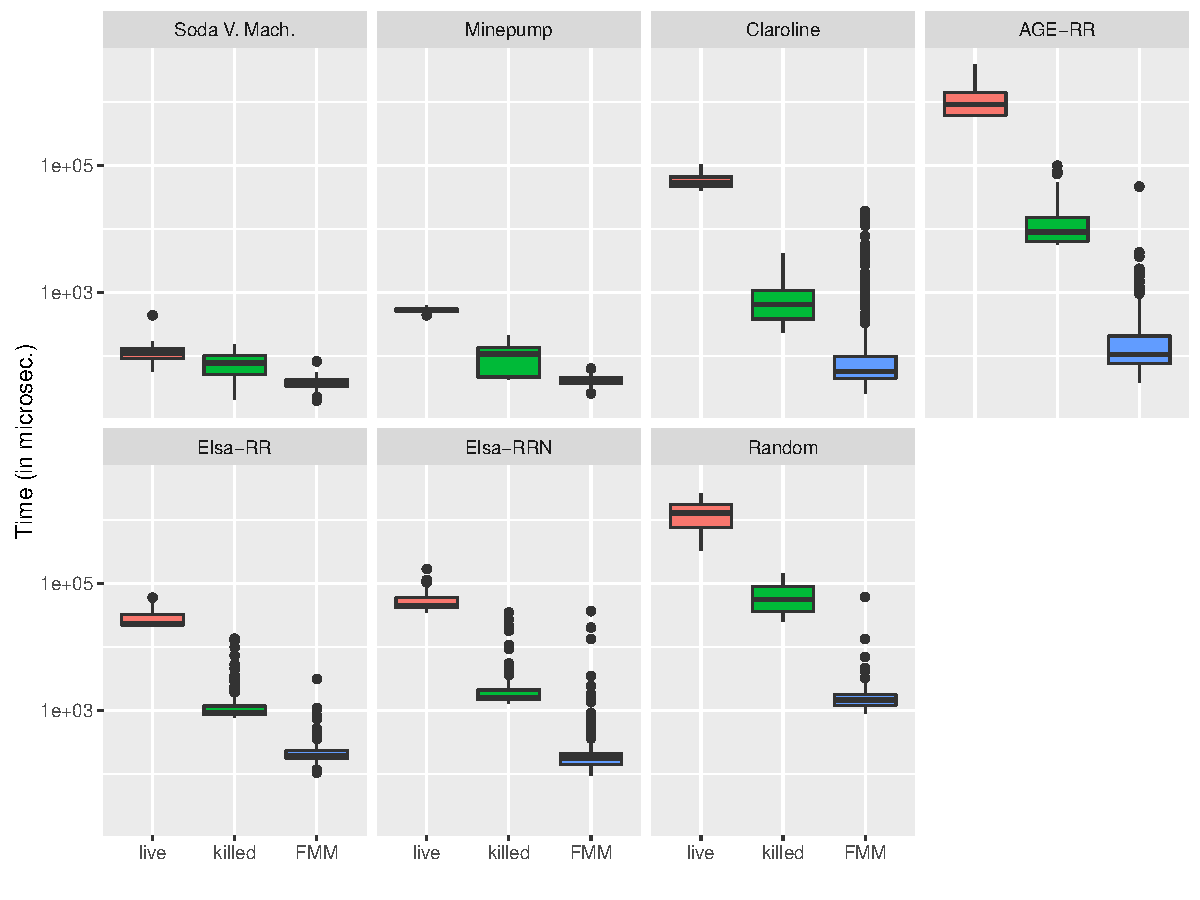
\includegraphics[width=0.98\textwidth]{mutants-exec-time}
	\caption{Execution time required by test cases to executed with live and killed mutants and the FMM mutants}
	\label{fig:assessment:mutantsexectime}
\end{figure}

Figure \ref{fig:assessment:mutantsexectime} presents the distribution of the test execution time (in logarithmic scale on the \textit{y} axis) for each studied model with a box plot. The first two columns represent the total execution time taken by each test case when executed on the live mutants and on the killed mutants according to the enumerative approach. The third box presents the execution time of the FMM (FMM approach). Note that while the killed mutants do not require a complete execution in the enumerative approach, it is required for the FMM mutants. This might provide an advantage to the enumerative approach. To assess this, we consider the killed and the live mutants separately. In all cases, we measure only the execution of the models, avoiding time bias due to I/O operations.
As the execution time of a test case partially depends on its size, the high number of outliers in Figure \ref{fig:assessment:mutantsexectime} is explained by the variation of the test cases sizes.

For the enumerative approach, executing a test case on mutants that will remain live takes more time than executing the same test cases on mutants that are killed. This was expected since killed mutants do not require a complete execution of the test case.
In both cases, the FMM execution runs faster, \ie running a test case on all the mutants at once is very fast, despite the more complex (needed) exploration of the FMM's FTS. Detailed statistics over the execution time of the models and mutation scores are presented in Annex \ref{apdx:fmm:exectime}. 

%----------------------
\subsection{Discussion}
%----------------------

\paragraph{Execution time:}
%--------------------------

Regarding \emph{RQ1}, the box plots of Figure \ref{fig:assessment:mutantsexectime} (and the values in Annex \ref{apdx:fmm:exectime}) confirm that the execution time required by the FMM approach is considerably lower than the time required by the enumerative approach. The difference escalates to several orders of magnitude when considering live mutants. The difference between family-based and enumerative approaches increases with the size of the model, indicating the improved scalability of our approach.

To evaluate the statistical significance, we use a Wilcoxon rank-sum test for the different models we considered: we obtain a $p$-value of $1.343e-09$ for the random model and $p$-values smaller than $2.2e-16$ for the other models, confirming the hypothesis that FMM significantly outperforms the enumerative approach, when considering $0.001$ significance level. 

\paragraph{Higher-order mutation:}
%---------------------------------

\begin{table}
\centering
\caption{All-order mutation scores}
\begin{small}
\begin{tabular}{l rrrrrrr}
\hline
\textbf{Model}	& \textbf{\# mutants}	& \multicolumn{3}{c}{\textbf{All-actions}}	& \multicolumn{3}{c}{\textbf{Random}}\\
	& 	& \textit{\#Lv.}	& \textit{MS} & \textit{Time}	&  \textit{\#Lv.}	& \textit{MS} & \textit{Time}	 \\
\hline 
Soda V. Mach.	&	127						& 1			& 0.99 & 1.10  & 1 & 0.99 & 17.67 \\
Minepump		&	8,388,607					& 1			& >0.99	& 1.84 & 1	& >0.99 & 15.72 \\
Claroline	&	5.49e+303	& \multicolumn{3}{c}{Timeout} & \multicolumn{3}{c}{Timeout} \\
AGE-RR		&	4.71e+956	 				& \multicolumn{3}{c}{Timeout} & \multicolumn{3}{c}{Timeout} \\
Elsa-RR		&	1.46e+194	& 2916	& >0.99	& 37.78  &  144	& >0.99 & 10.19 \\
Elsa-RRN		&	7.61e+286	& 36			& >0.99	& 150.32  & 16		& >0.99 & 83.04 \\
Random 1		&	2.62e+2577					& \multicolumn{3}{c}{Memory overflow} & \multicolumn{3}{c}{Memory overflow} \\
\hline
\end{tabular}
\end{small}
\label{tab:experiment:fmmexec:norderscore}
\end{table}

Table \ref{tab:experiment:fmmexec:norderscore} presents the number of all-order mutants for our models, the number of mutants live after executing the random and all-actions test sets (computed using SAT4J 2.3.5), and their mutation score. For each test set and model, the table records the number of possible mutants (\textit{\# mutants}), the number of live mutants after the test set execution (\textit{\#Lv.}), the mutations score (\textit{MS}) and the SAT computation time (\textit{Time}) in seconds. \textit{Memory Overflow} denotes an overflow during SAT solving, improving this step by, for instance, reducing the boolean formula to process is part of our future work. Columns 5 and 8 give the SAT-solving computation time (we set a timeout of 12 hours). 

Overall, our results suggest that higher-order mutation under the FMM scheme is tractable, answering positively to \emph{RQ2}.  In particular, all-order mutation achieves very good mutation scores ($MS \geq 0.99$) when compared to first-order mutation when this score can be computed. In our future work, we intend to: improve the scalability of mutation score computation; and assess the practical relevance of higher-order in test sets comparison.

Only one mutant is live for the soda vending machine and the Minepump products. This mutant is a first order mutant resulting from the TAD operator. Indeed, the TAD operator adds new transition which cannot be detected by test cases solely selected from the original LTS, since this transition does not exist in this model. All-order mutation enables to quickly kill mutants of any order an to focus on the interesting ones from a selective mutation perspective. For example, the 2,916 remaining live mutants resulting from the execution of the all-action test suite are relevant to study the mutation operators involved. Of course, they can also be used to select test cases killing them in order to augment the test suite. Exploring all-order mutation score in selective mutation or test case selection scenarios are part of our future work.  

%----------------------------------
\subsection{Threats to validity}
%----------------------------------

%\paragraph{Construct validity:}
%------------------------------

We chose to apply mutants for $1/10$ of the states and/or transitions of the mutated model. This might result in more (or less) mutants than needed for the larger models. However, this is expected when using mutation. Additionally, since model-based mutation is applied to the system's abstraction, abstract actions represent many concrete actions. It is therefore important to ensure a good coverage of most of the model actions.

TS and FTS executions are different, and do not use the same algorithms. In order to decrease the bias in measuring execution time, both executions of the models have been done using VIBeS, our \emph{Variability Intensive Behavioural teSting framework} Java implementation. The two execution classes are different but use a variant of the same algorithm described in Section \ref{sec:FMM}. Moreover, we used the \texttt{Stopwatch} Java class to measure the call to the execute method (\ie model loading and result writing time have been omitted). 
Finally, we ran each test case 3 times on each mutant model (LTSs and FMMs) to avoid bias due to process concurrency.

%\paragraph{External validity:}
%%------------------------------
%
%We cannot guarantee that our results are generalizable to all behavioural models. However, we recall the diversity of the model sources (hand-crafted, reverse-engineered, and randomly generated to match real system state-space) as well as the diversity of considered systems.


%%%%%%%%%%%%%%%%%%%%%%%%%%%%%%%%%%%%
\section{Mutant equivalence analysis}
%%%%%%%%%%%%%%%%%%%%%%%%%%%%%%%%%%%%

\label{sec:experiment:mutequiv}
% apdx:fmm:equivalence

\glsreset{ALE} \glsreset{RS} \glsreset{BS}  \glsreset{WM} \glsreset{SM}  

This section presents our empirical assessment of the \gls{ALE}, \gls{RS}, and \gls{BS} approaches to detect equivalent mutants \cite{Devroey2017}. As in Section \ref{sec:EMP}, we adopt a product-based strategy: mutants are generated from products, derived from the case studies defined in Chapter \ref{chap:casestudies} (and from 4 additional randomly generated models). To conduct this assessment, we define the following research questions:
\begin{itemize}
\item \textbf{\textit{Random/biased simulations and ALE} (RQ.1) } What is the impact of weak and strong mutation on BS/RS \textit{vs}. ALE performance?
\item \textbf{\textit{Non-equivalent mutant detection} (RQ.2) } How many non-equivalent mutants are effectively detected by the RS and BS appro\-aches?
\item \textbf{\textit{Worst case scenario} (RQ.3) } What are the worst case execution times for the ALE and BS/RS approaches?
\end{itemize}

%----------------------
\subsection{Setup}
%-----------------------

To answer these RQs, we consider several models of different kinds of systems and apply the following procedure to each of them:
\begin{enumerate}
\item we generate a set of mutants from the model using the operators presented in Annex \ref{apdx:fmm:operators} for orders 1, 2, 5, and 10;
\item for each order, we sample 100 non-equivalent mutants (using the ALE algorithm to guarantee non-equivalence) to form the mutant set $M$;
\item for each mutant in $M$, we measure the execution time and result of: 3 executions of weak mutation random and biased search (WM RS/BS), and 3 executions of strong mutation-biased search (SM BS) algorithms\footnote{As explained in Section \ref{sec:EMP}, SM RS is not considered for the assessment due to the poor results during our initial attempts.} with 4 different values of $\delta$ and $\epsilon$; and the executions of the ALE algorithm.
\end{enumerate}
In the following we detail the different steps of the procedure. The assessment has been performed on a Debian 3.16.7 x86\_64 GNU/Linux running on a 16 cores, 2.2 GHz, 16Gb RAM virtual machine.

\paragraph{Models:}
%------------------

We carry out the assessment on 12 different models coming from different sources and with varying size. The models are:
\begin{itemize}
\item a soda vending machine product (\textit{S. V. Mach.}) that includes all features;
\item a card payment terminal product (\textit{C. P. Term.}) that includes all features;
\item a Minepump product (\textit{Mine\-pump}) that includes all features;
\item a Claroline product (\textit{Claroline}) that includes all features and an \textit{Admin} user;
\item four WordPress products (\textit{AGE-RR}, \textit{AGE-RRN}, \textit{Elsa-RR}, and \textit{Elsa-RRN}) that include all features of their respective feature models;
\item four random models (Random 1-4).
\end{itemize}

\paragraph{Mutant generation and sampling:}
%-----------------------------------------

First-order mutants are generated using the operators presented in Annex \ref{apdx:fmm:operators}. Each operator is applied (arbitrarily) 10 times on the \textit{S.\-V.\-Mach.}, \textit{C.\-P.\-Term.}, and \textit{Mine\-pump} products. Due to the small size of the models, applying the same mutation operator more than 10 times is not relevant. Operators are also applied (arbitrarily) 500 times on the other models. In the same way, \textit{N}-order mutants (with $N$ equal to 2, 5, or 10 in our case) are generated by applying the same operators 10 or 500 times (depending on the model) on ($N-1$)-order mutants.
After the generation, we perform a random sampling of 100 mutants (when available) for orders 1, 2, 5, and 10, giving us a set $M$ with 370 mutants for the \textit{S.\-V.\-Mach.}, \textit{C.\-P.\-Term.}, and \textit{Mine\-pump} models, and 400 mutants for the other models.
To ease mutant generation, we use the compact representation provided by FMMs. 

\paragraph{Non-determinism:}
%--------------------------

We checked all the 4710 mutants and found that only 3.54\% of them are non-deterministic (\ie there exists a sequence of actions for which there is at least two possible paths in the mutant). Nevertheless, there is a great disparity amongst models as the non-determinism rate varies from 0\% for \textit{Elsa-RRN} to 15.5\% for \textit{Claroline}. Higher-order mutation greatly influenced non-determinism rates: the sole order 10 is responsible for 53\% of all non-deterministic mutants. In terms of mutation operators, TAD accounts for a large majority  of non-deterministic first-order mutants (78\%) and AEX for the remaining 22\%.  At higher orders, these two operators are largely involved. They are absent only in the \textit{Minepump} model where TDE and AMI appear for two non-deterministic mutants. 

\paragraph{Algorithm execution:}
%------------------------------

To run the language equivalence algorithms (for WM and SM), we use the HKC library \cite{hkc}, an OCaml implementation of the ALE  algorithm \cite{Bonchi2013} compiled using OCamlbuild. This tool handles non-deterministic TSs using different strategies: the automata may be processed either forward of backwards, and the exploration strategy may be breadth-first or depth-first. For each mutant, we execute the HKC library using each of the 4 possible configurations. The input models and their mutants have been transformed from our XML format to the Timbuk input format supported by HKC.

The random and biased simulation algorithms are implemented in Java using multi-threading to parallelize trace selection and execution as described in Algorithm \ref{algo:fmm:randomequiv} (lines \ref{line:fmm:randomequiv:posrandomselect}, \ref{line:fmm:randomequiv:posexec}, \ref{line:fmm:randomequiv:negrandomselect}, and \ref{line:fmm:randomequiv:negexec}). In our experiments, we set up the algorithm with 4 threads and run 4 instances in parallel on our virtual machine with 16 cores.
We run the simulation algorithms with 4 different values of $\delta$ and $\epsilon$ determining the number of traces selected and executed ($N$ in Algorithm \ref{algo:fmm:randomequiv}): 
\begin{itemize}
\item RS1/BS1: ($\delta=1e-10$, $\epsilon=0.01$, $N=1,897,519$);
\item RS2/BS2: ($\delta=1e-10$, $\epsilon=0.1$, $N=18,975$);
\item RS3/BS3: ($\delta=1e-5$, $\epsilon=0.1$, $N=9,764$);
\item RS4/BS4: ($\delta=1e-1$, $\epsilon=0.1$, $N=2,396$).
\end{itemize}

For all the simulation configurations and all models, we fixed the trace length $k$ to 3,000, which was our compromise between performance and non-equivalence detection: setting $k$ to BFS height led to crashes in some cases. In order to answer RQ3, we also run each algorithm (RS1/BS1 to RS4/BS4, plus the 4 possible ALE configurations) with the model itself as the mutant. Those (unrealistic) equivalent detection runs between the model and itself are only used to approximate the worst computation time of the different algorithms.

%-----------------------------------
\subsection{Results and discussion}
%-----------------------------------

\paragraph{Random/biased simulations and ALE:}
%--------------------------------------------

\begin{figure}[t]
	\centering
	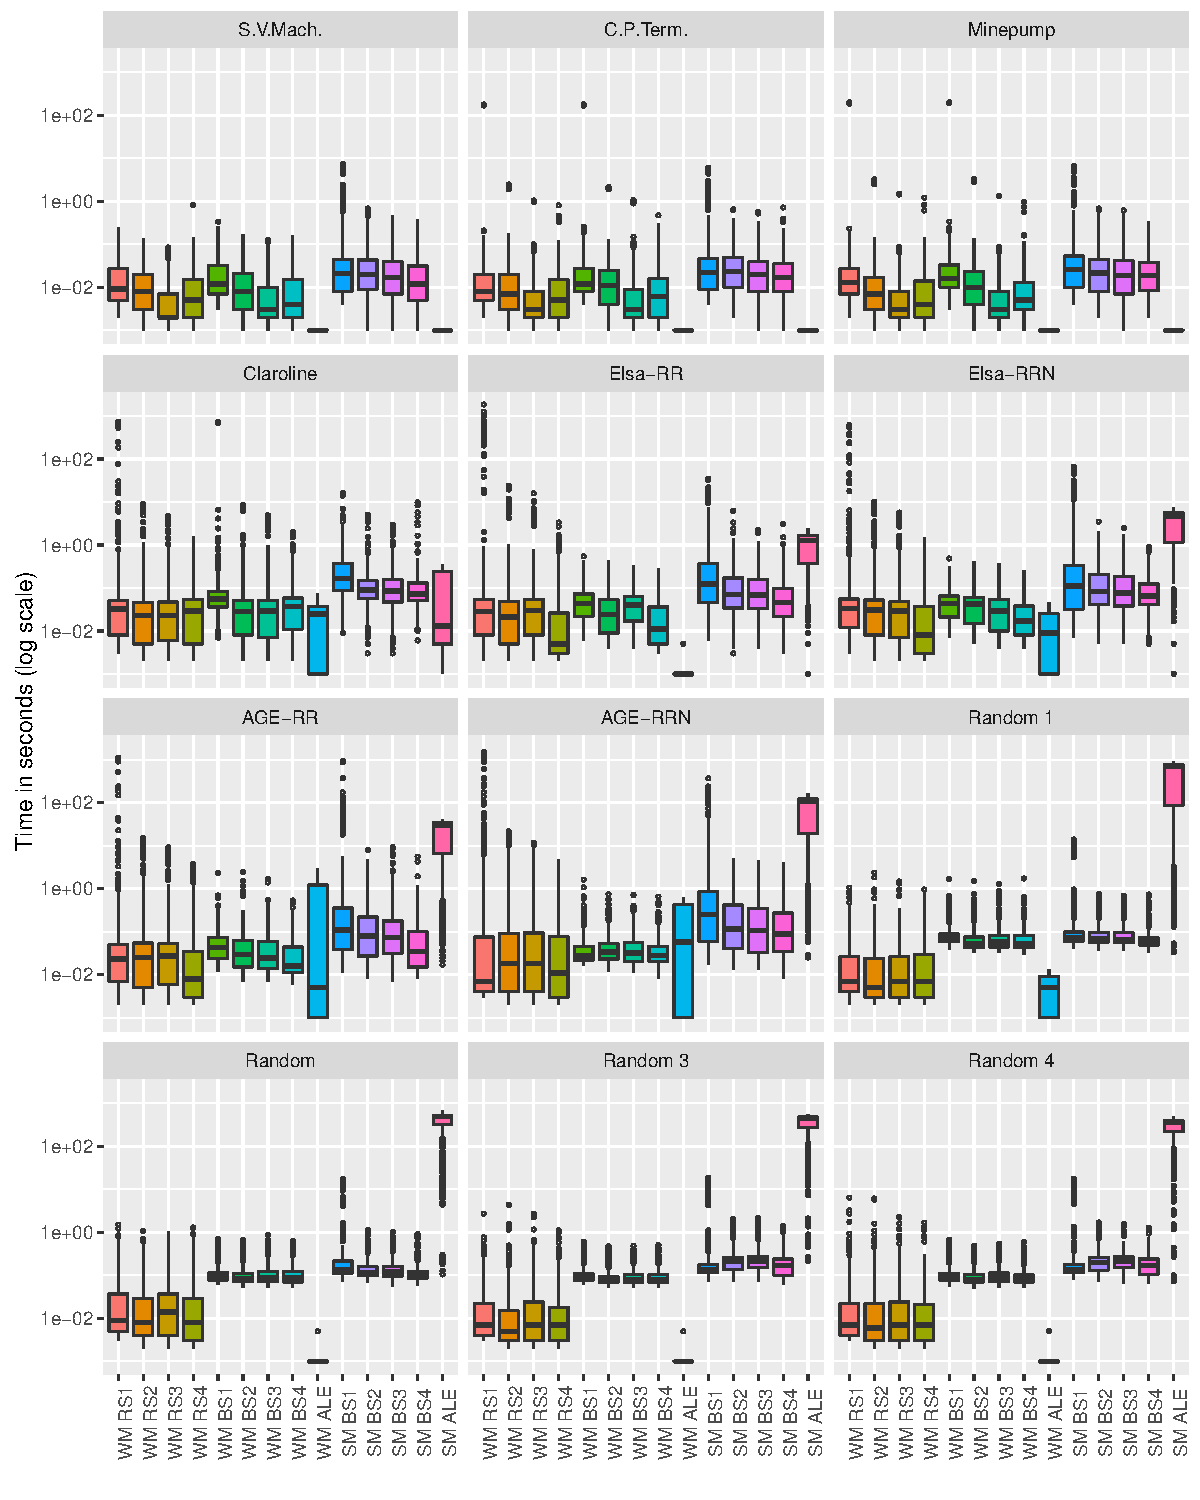
\includegraphics[width=0.98\textwidth]{mutants-equiv-time}
	\caption{Execution time of the equivalent mutant detection approaches}
	\label{fig:assessment:mutantsequivtime}
\end{figure}

Figure \ref{fig:assessment:mutantsequivtime} presents the execution time per mutant of the studied algorithms, which is detailed in the Appendix. Regarding weak mutation scenarios, the ALE approach is the fastest in all cases in eleven of our models. On the \textit{AGE-RN} model,  biased simulations are faster for the largest numbers of runs.  However, the results are at the limit of non-significance (see Table \ref{tab:assessment:mutantsequivwmpvalues}), so that the only clearly significant result is for \emph{BS1} on this model. For \textit{AGE-RNN}, execution times for  biased simulations are non-significant. Random simulations are also faster than ALE on \textit{AGE-RRN} but only certain settings are significant. We thus conclude that the ALE approach is more interesting in terms of execution time. When we compare the two forms of simulations, for the smallest models, biased simulations are either on par for the smallest models or slightly better. Additional computations such as the breath-first search used for biased simulation do not cause significant overhead. For the largest random models, random simulations are faster. In these cases, the overhead of computing infected states and paths that cover these states is greater and random simulation is faster.  However, lower standard deviations for biased simulation execution times over random ones make the BS approach easier to use.
       
Regarding strong mutation, several observations can be made. First, random simulations provide very high execution times compared to biased simulations or the ALE algorithm (the analysis of one model is stopped after one hour). This may be due to the difficulty to reach the initial state again when performing random walks in the TSs.
Second, biased simulations are faster than ALE executions for models larger than 300 states. On the largest models, biased simulations can be up to 1,000 times faster. We thus conclude that these are the most interesting situations in which to use BS, for mutation analysis.  On smaller models, the ALE algorithm's performance is quite impressive and therefore should be privileged.              

\paragraph{Non-equivalent mutant detection:}
%--------------------------------------------

\begin{figure}
	\centering
	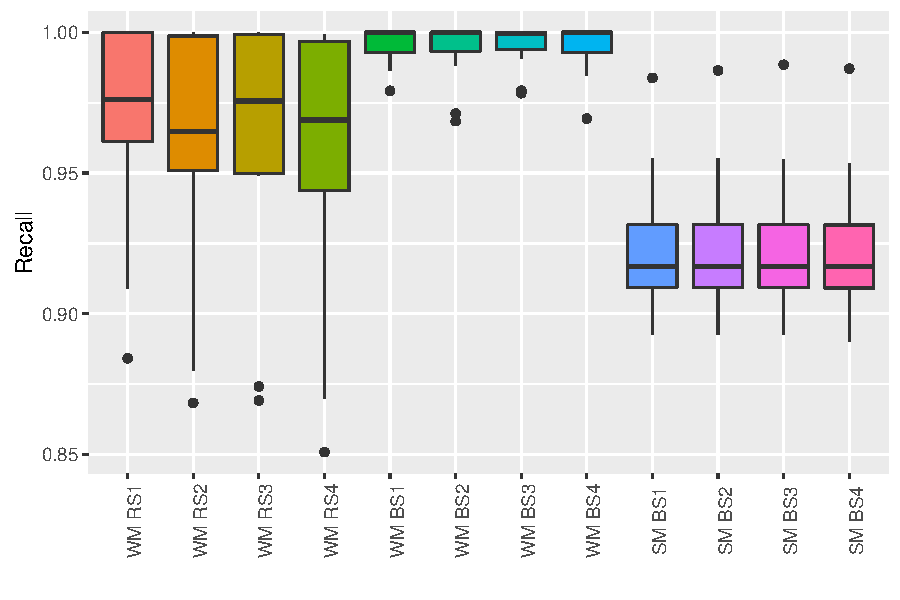
\includegraphics[width=90mm]{mutants-equiv-recall}
	\caption{Non-equivalent mutant classification recall}
	\label{fig:assessment:mutantsequivrecall}
\end{figure}

To answer RQ2, we compute the non-equi\-va\-lent mutant classification recall of the BS/RS algorithms (in Figure \ref{fig:assessment:mutantsequivrecall}), \ie the percentage of non-equi\-va\-lent mutants detected by the BS/RS amongst the selected mutants. By construction, the ALE algorithm has a recall of 100\%, it is therefore not shown here. It is also noted that the precision is 100\% since all the non-equivalent mutants detected are indeed killable, by construction of our mutant set. 

All our simulations obtain a recall higher than 85\%, with a clear advantage for biased simulations which  never achieve worse than  95\% for the weak mutation scenario.  As for time, deviation in the recall is smaller for biased simulations thus making the approach more predictable in addition of being more reliable. We also observe that the random simulations are more sensitive to the number of runs: we need more of them to discover discrepancies by luck. This effect cannot be observed for biased simulations. A possible explanation is that the number of runs required to cover infected states with traces is lower than the number we provided.  

For strong mutation, the BS approach's recall decreases to around 92\% ($\overline{recall}=92$\%, $\sigma=3$\%): amongst the 5113  non-equi\-va\-lent mutant non-detections (over a total of 64529 non-equi\-va\-lent mutant evaluations), 1905 (37\%) were TAD mutants, 1755 (34\%) were WIS mutants, 545 (11\%) were TDE mutants, and 459 (9\%) were 2nd-order TAD mutants (\textit{i.e.}, TAD-TAD mutants); the rest of non-equi\-va\-lent mutants not detected is distributed amongst different operators with less than 2\% for each. This decrease may be due to the difficulty to find a path to the initial state: for strong mutation, the BS trace selection algorithm will consider traces starting from, and ending in, the initial state. This means that mutations creating (TAD) or modifying (TDE) a back-level transition will not be detected using SM BS. Concerning WIS mutants, we believe that, as the WIS operator only changes the initial state of the TS, the set of infected states ($S_{infect}$) is empty, which is equivalent in our implementation of SM BS to considering all the states infected.

\paragraph{Worst case scenario:}
%--------------------------------

\begin{figure}[t]
	\centering
	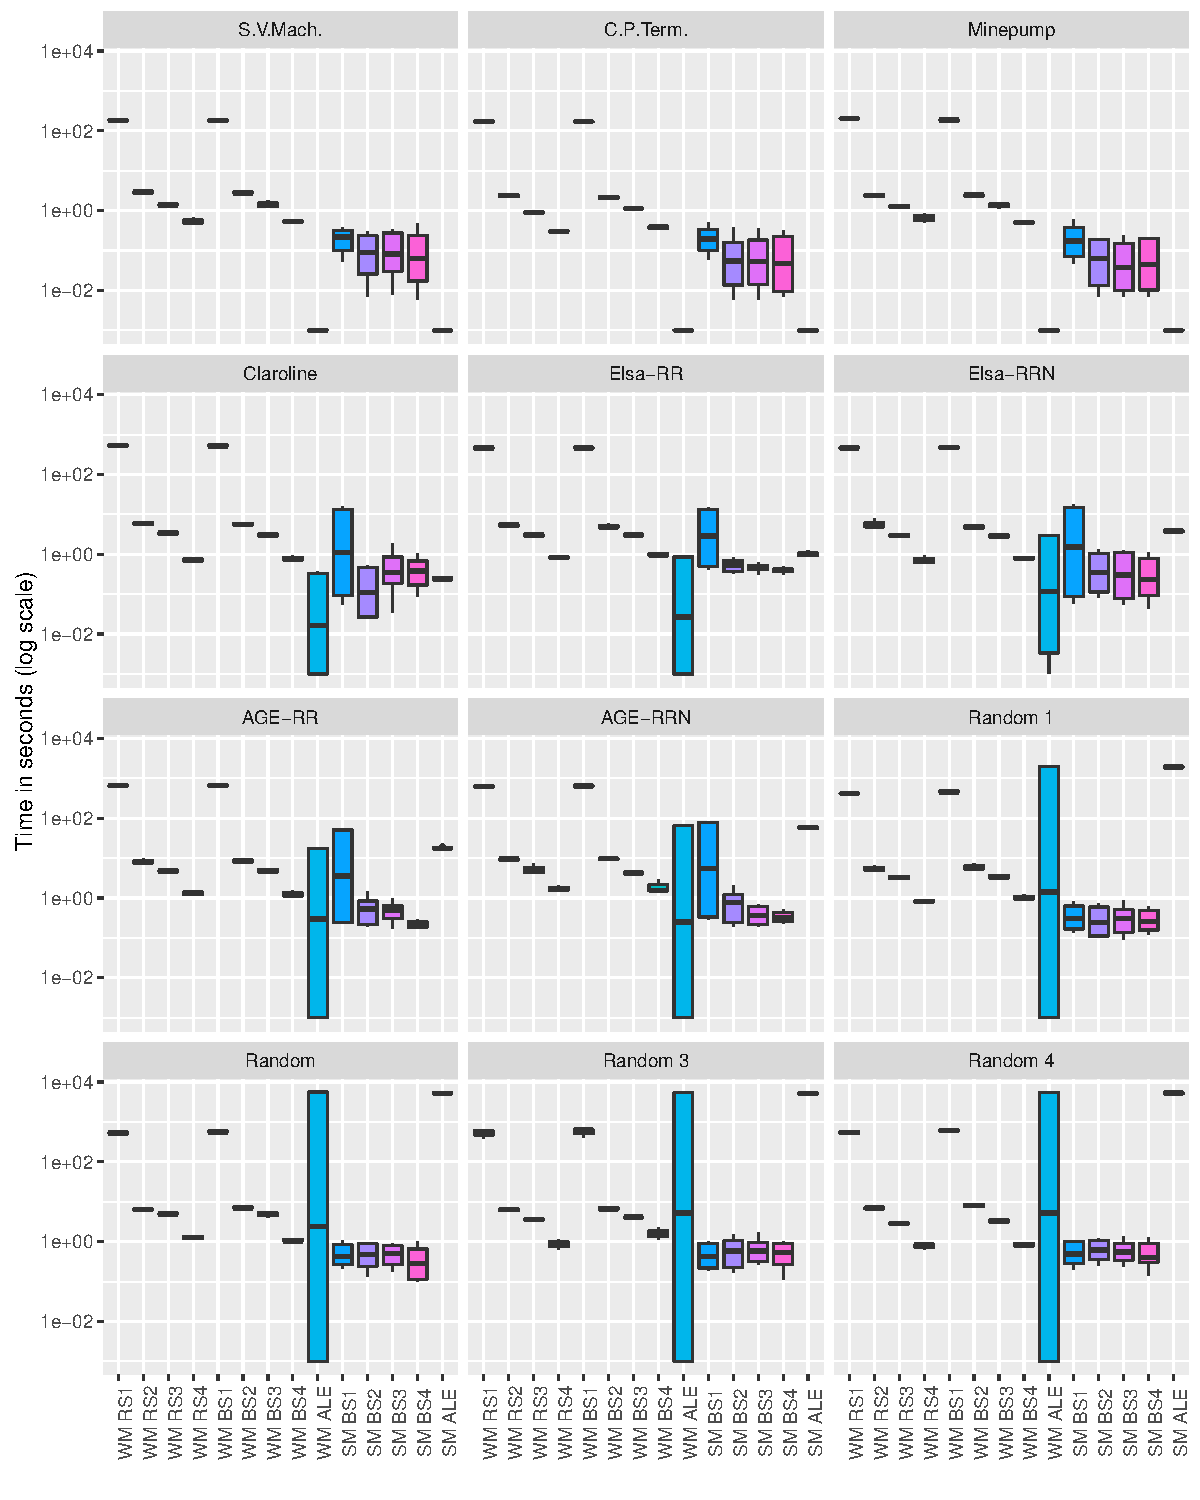
\includegraphics[width=0.98\textwidth]{mutants-equiv-worst}
	\caption{Worst execution time of the equivalent mutant detection using the model itself as mutant}
	\label{fig:assessment:mutantsequivworst}
\end{figure}

Figure \ref{fig:assessment:mutantsequivworst} presents a compact view of the worst execution time of the different algorithms (RQ3). We grouped the different results by the kind of model: embedded system, web-application, or randomly generated model. As expected, the RS/BS execution time is directly correlated to the $\delta$ and $\epsilon$ values: a lower number of traces selected and executed ($N$) takes less time. Overall, the time of the ALE executions grows with the size of the model, reaching 5660 seconds (more than one and a half hour) for the worst WM ALE execution time on the Random~2 model.

%------------------------------
\subsection{Threats to validity}
%------------------------------

\paragraph{Construct validity:}
%-----------------------------

The RS/BS $\delta$ and $\epsilon$ values have been arbitrarily chosen. The first values (RS1/BS1: $\delta=1e-10$, $\epsilon=0.01$) are the same as in H\'erault \etal~\cite{Herault2004}. As the number of traces selected and executed $N$ equals to $\frac{8\log(2/\delta)}{\epsilon^2}$, we chose to run the algorithm with 3 higher parameters values in order to reduce $N$. We cannot guarantee that our parameter values are relevant for any model. They will rather depend on the model size, the desired approximation ($\epsilon$) and confidence ($\delta$), and the time budget allowed for the equivalence analysis.

To the best of our knowledge, the HKC library \cite{hkc} was the only publicly available tool able to perform ALE checking on non-deterministic TSs. We cannot guarantee that there are no other other tools providing the same features with lower execution time. 
To avoid bias in the random selections in the RS/BS algorithms, we execute each configuration of the different algorithms 3 times.

%\paragraph{External validity:}
%%----------------------------
%
%We cannot guarantee that our results are generalizable to all behavioural models. However, we recall the diversity of the model sources (hand-crafted, reverse-engineered, and randomly generated to match real system state-space) as well as the diversity of the considered systems. Variations in performance of the algorithms also suggest mitigation of this threat.

\paragraph{Conclusion validity:}
%-------------------------------

To confirm our observations on the recall of the RS/BS algorithms, we test the null hypothesis between the outputs of our algorithm (the mutant is equivalent/non-equivalent) and a random equivalent/non-equivalent assignment using a Wilcoxon rank sum test. The p-value lower than 2.2e-16\footnote{Due to floating point precision, value $2.2e-16$ corresponds to the smallest possible p-value computable with R.} discredits the null hypothesis showing that the equivalent/non-equivalent detection recall is significant.

\begin{table}
	\centering
	\caption{P-values of the Wilcoxon rank sum test between the WM RS/BS execution times and the WM ALE execution times.}
	\label{tab:assessment:mutantsequivwmpvalues}
	\begin{small} 
\begin{tabular}{lcccc}
%\label{table:WM-pval}
\hline 
\textbf{Model} & \textbf{ WM RS1 } & \textbf{ WM RS2 } & \textbf{ WM RS3 } & \textbf{ WM RS4 } \\ 
\hline 
S.V.Mach.   & $\le 2.2e-16$ & $\le 2.2e-16$ & $\le 2.2e-16$ & $\le 2.2e-16$ \\ 
C.P.Term.   & $\le 2.2e-16$ & $\le 2.2e-16$ & $\le 2.2e-16$ & $\le 2.2e-16$ \\ 
Minepump    & $\le 2.2e-16$ & $\le 2.2e-16$ & $\le 2.2e-16$ & $\le 2.2e-16$ \\ 
Claroline   & $\le 2.2e-16$ & $\le 2.2e-16$ & $\le 2.2e-16$ & $\le 2.2e-16$ \\
Elsa-RR     & $\le 2.2e-16$ & $\le 2.2e-16$ & $\le 2.2e-16$ & $\le 2.2e-16$ \\
Elsa-RRN   & $\le 2.2e-16$ & $\le 2.2e-16$ & $\le 2.2e-16$ & $\le 2.2e-16$ \\
AGE-RR   & $2.866e-03$ & $9.676e-03$ & $2.021e-02$ & $\mathbf{3.249e-01}$ \\
AGE-RRN   & $\mathbf{8.143e-02}$ & $8.379e-04$ & $6.981e-04$ & $2.162e-02$ \\
Random 1   & $\le 2.2e-16$ & $\le 2.2e-16$ & $\le 2.2e-16$ & $\le 2.2e-16$ \\
Random 2   & $\le 2.2e-16$ & $\le 2.2e-16$ & $\le 2.2e-16$ & $\le 2.2e-16$ \\
Random 3   & $\le 2.2e-16$ & $\le 2.2e-16$ & $\le 2.2e-16$ & $\le 2.2e-16$ \\
Random 4   & $\le 2.2e-16$ & $\le 2.2e-16$ & $\le 2.2e-16$ & $\le 2.2e-16$ \\
\hline 
\end{tabular} 
\end{small}

\vspace{1em}

\begin{small} 
\begin{tabular}{lcccc}
%\label{table:WM-pval}
\hline 
\textbf{Model} & \textbf{ WM BS1 } & \textbf{ WM BS2 } & \textbf{ WM BS3 } & \textbf{ WM BS4 } \\ 
\hline 
S.V.Mach.   & $\le 2.2e-16$ & $\le 2.2e-16$ & $\le 2.2e-16$ & $\le 2.2e-16$\\ 
C.P.Term.   & $\le 2.2e-16$ & $\le 2.2e-16$ & $\le 2.2e-16$ & $\le 2.2e-16$\\ 
Minepump    & $\le 2.2e-16$ & $\le 2.2e-16$ & $\le 2.2e-16$ & $\le 2.2e-16$\\ 
Claroline   & $\le 2.2e-16$ & $\le 2.2e-16$ & $\le 2.2e-16$ & $\le 2.2e-16$\\ 
Elsa-RR     & $\le 2.2e-16$ & $\le 2.2e-16$ & $\le 2.2e-16$ & $\le 2.2e-16$\\ 
Elsa-RRN    & $\le 2.2e-16$ & $\le 2.2e-16$ & $\le 2.2e-16$ & $\le 2.2e-16$\\ 
AGE-RR      & $9.107e-03$ & $4.744e-02$ & $\mathbf{6.405e-02}$ & $\mathbf{1.382e-01}$\\ 
AGE-RRN     & $\mathbf{5.991e-01}$ & $\mathbf{7.076e-01}$ & $\mathbf{5.674e-01}$ & $\mathbf{5.168e-01}$\\ 
Random 1    & $\le 2.2e-16$ & $\le 2.2e-16$ & $\le 2.2e-16$ & $\le 2.2e-16$\\ 
Random 2    & $\le 2.2e-16$ & $\le 2.2e-16$ & $\le 2.2e-16$ & $\le 2.2e-16$\\ 
Random 3    & $\le 2.2e-16$ & $\le 2.2e-16$ & $\le 2.2e-16$ & $\le 2.2e-16$\\ 
Random 4    & $\le 2.2e-16$ & $\le 2.2e-16$ & $\le 2.2e-16$ & $\le 2.2e-16$\\ 
\hline 
\end{tabular} 
\end{small}

\end{table}

To confirm the statistical difference between the execution times of the RS/BS and ALE algorithms, we test the null hypothesis between RS/BS execution time and ALE execution time for weak and strong mutation for each of our input models using a Wilcoxon rank sum test. For weak mutation, the results of this statistical test are shown in Table \ref{tab:assessment:mutantsequivwmpvalues}: for every model except \textit{AGE-RR}/\textit{AGE-RRN} models, the p-value is lower than 2.2e-16, discrediting the null hypothesis and showing a significant difference in the execution times. The execution times of \textit{AGE-RR}/\textit{AGE-RRN} model are only significant for RS1 to RS3, BS1, and BS3 (for \textit{AGE-RR}); and RS2 to RS4 (for \textit{AGE-RRN}). For strong mutation, all the p-values were lower than 2.2e-16, showing a significant difference in execution time between the BS algorithm and the ALE algorithm in a strong mutation scenario.


%------------------------------
\subsection{Lessons learned}
%------------------------------

From our experiment we draw the following lessons: 
\begin{inparaenum}
\item regarding weak mutation and independently of the size or nature of the models, the ALE approach provides faster and exact answers. This indicates that state-of-the-art language equivalence algorithms can be used successfully for such a task.
\item Regarding strong mutation, biased random simulations are of interest for the web and the random models, and gains increase with the size (from one to three orders of magnitude).  Recalls of 90\% and above allow to use such simulations as reasonably reliable fast filters to discard non-equivalent mutants, leaving to ALE algorithms ``difficult" cases so as to accelerate the analysis of large mutants bases.
\item Biased simulations are more predictable in terms of execution time and recall. Additionally, drastically increasing the number of runs does not affect their performance as opposed to random simulations.    
\item The configuration of the ALE algorithm (forward/backward processing, or breadth-first or depth-first exploration) has very little influence on the total execution time (regarding equivalent mutant detection). This may be explained by the fact that mutations occur randomly and therefore do not privilege any graph traversal strategy.  
\end{inparaenum}


%%%%%%%%%%%%%%%%%%%%%%%%%%%%%%%%%%%%
\section{Wrap up}
%%%%%%%%%%%%%%%%%%%%%%%%%%%%%%%%%%%%

This chapter presents the empirical assessment and their results validating the the selection criteria and mutation analysis described in Chapters \ref{chap:coverage} and \ref{chap:mutation}. Future work include generalisation of the results by using all the case studies from Chapter \ref{chap:casestudies} for each assessment and comparison of the different test suite selection criteria using mutation analysis. 










%%%%%%%%%%%%%%%%%%%%%%%%%%%%%%%%%%%%%%%%%%%%%%%%%%%%%%%%%
\part{Implementation}
%%%%%%%%%%%%%%%%%%%%%%%%%%%%%%%%%%%%%%%%%%%%%%%%%%%%%%%%%
\label{part:implem}

\chapter{Variability Intensive Behavioural teSting framework}
\chaptermark{VIBeS}
\label{chap:vibes}
\glsreset{VIBeS}


\gls{VIBeS} is the framework we developed to support the testing activities described in this thesis. It is designed as a Maven project, decomposed in several Maven modules, to allow flexibility and rapid prototyping. In total, \gls{VIBeS} has around 16,000 lines of code distributed amongst 307 Java classes. It is released (since its inception) under the MIT license and publicly available on GitHub (\url{https://github.com/xdevroey/vibes}). Each assessment from Chapter \ref{chap:assessment} has been performed using one particular version of \gls{VIBeS} and each one of those versions is available in the Maven Central Repository\footnote{See \url{https://search.maven.org}.}. This allows one to reproduce the assessments using the same version of the tool enforcing reproducibility of our results. 

This chapter presents the architecture (in Section \ref{sec:vibesarchitecture}) and the usages (in Section \ref{sec:vibesusages}) of the last version (v.1.1.6) of \gls{VIBeS}. Section \ref{sec:vibesperspectives} concludes this chapter and presents future developments.

%%%%%%%%%%%%%%%%%%%%%%%%%%%%%%
\section{Architecture}
%%%%%%%%%%%%%%%%%%%%%%%%%%%%%%

\label{sec:vibesarchitecture}

\gls{VIBeS} is built as a set of \emph{Maven modules}. Maven is a industrial build management tool build upon the \textit{convention over configuration} philosophy \cite{Sonatype2011}:
\begin{quote}
``Convention over configuration is a simple concept: systems, libraries, and frameworks should assume reasonable defaults. Without requiring unnecessary configuration, systems should ``just work''.''
\end{quote}
This philosophy allows to have a flexible and extensible (using Maven plugins) build process, while ensuring a minimal configuration effort for the developer. 
Maven is able to build Java application and libraries (called \emph{artefacts} in the Maven world), including compilation, JUnit test execution, and Jar packaging. Each artefact is described by a \emph{\gls{POM}}, containing a unique identifier and other information about the artefact, dependencies to other artefacts, \etc The artefact unique identifier is a triplet: a \emph{group} identifier; an \emph{artefact} identifier; and a \emph{version} number. For instance, the version of \gls{VIBeS} described is this chapter is the artefact \texttt{be.unamur.info:vibes:1.1.6}, where the group identifier, artefact identifier, and version number are separated by ':'.

\begin{figure}
	\centering
	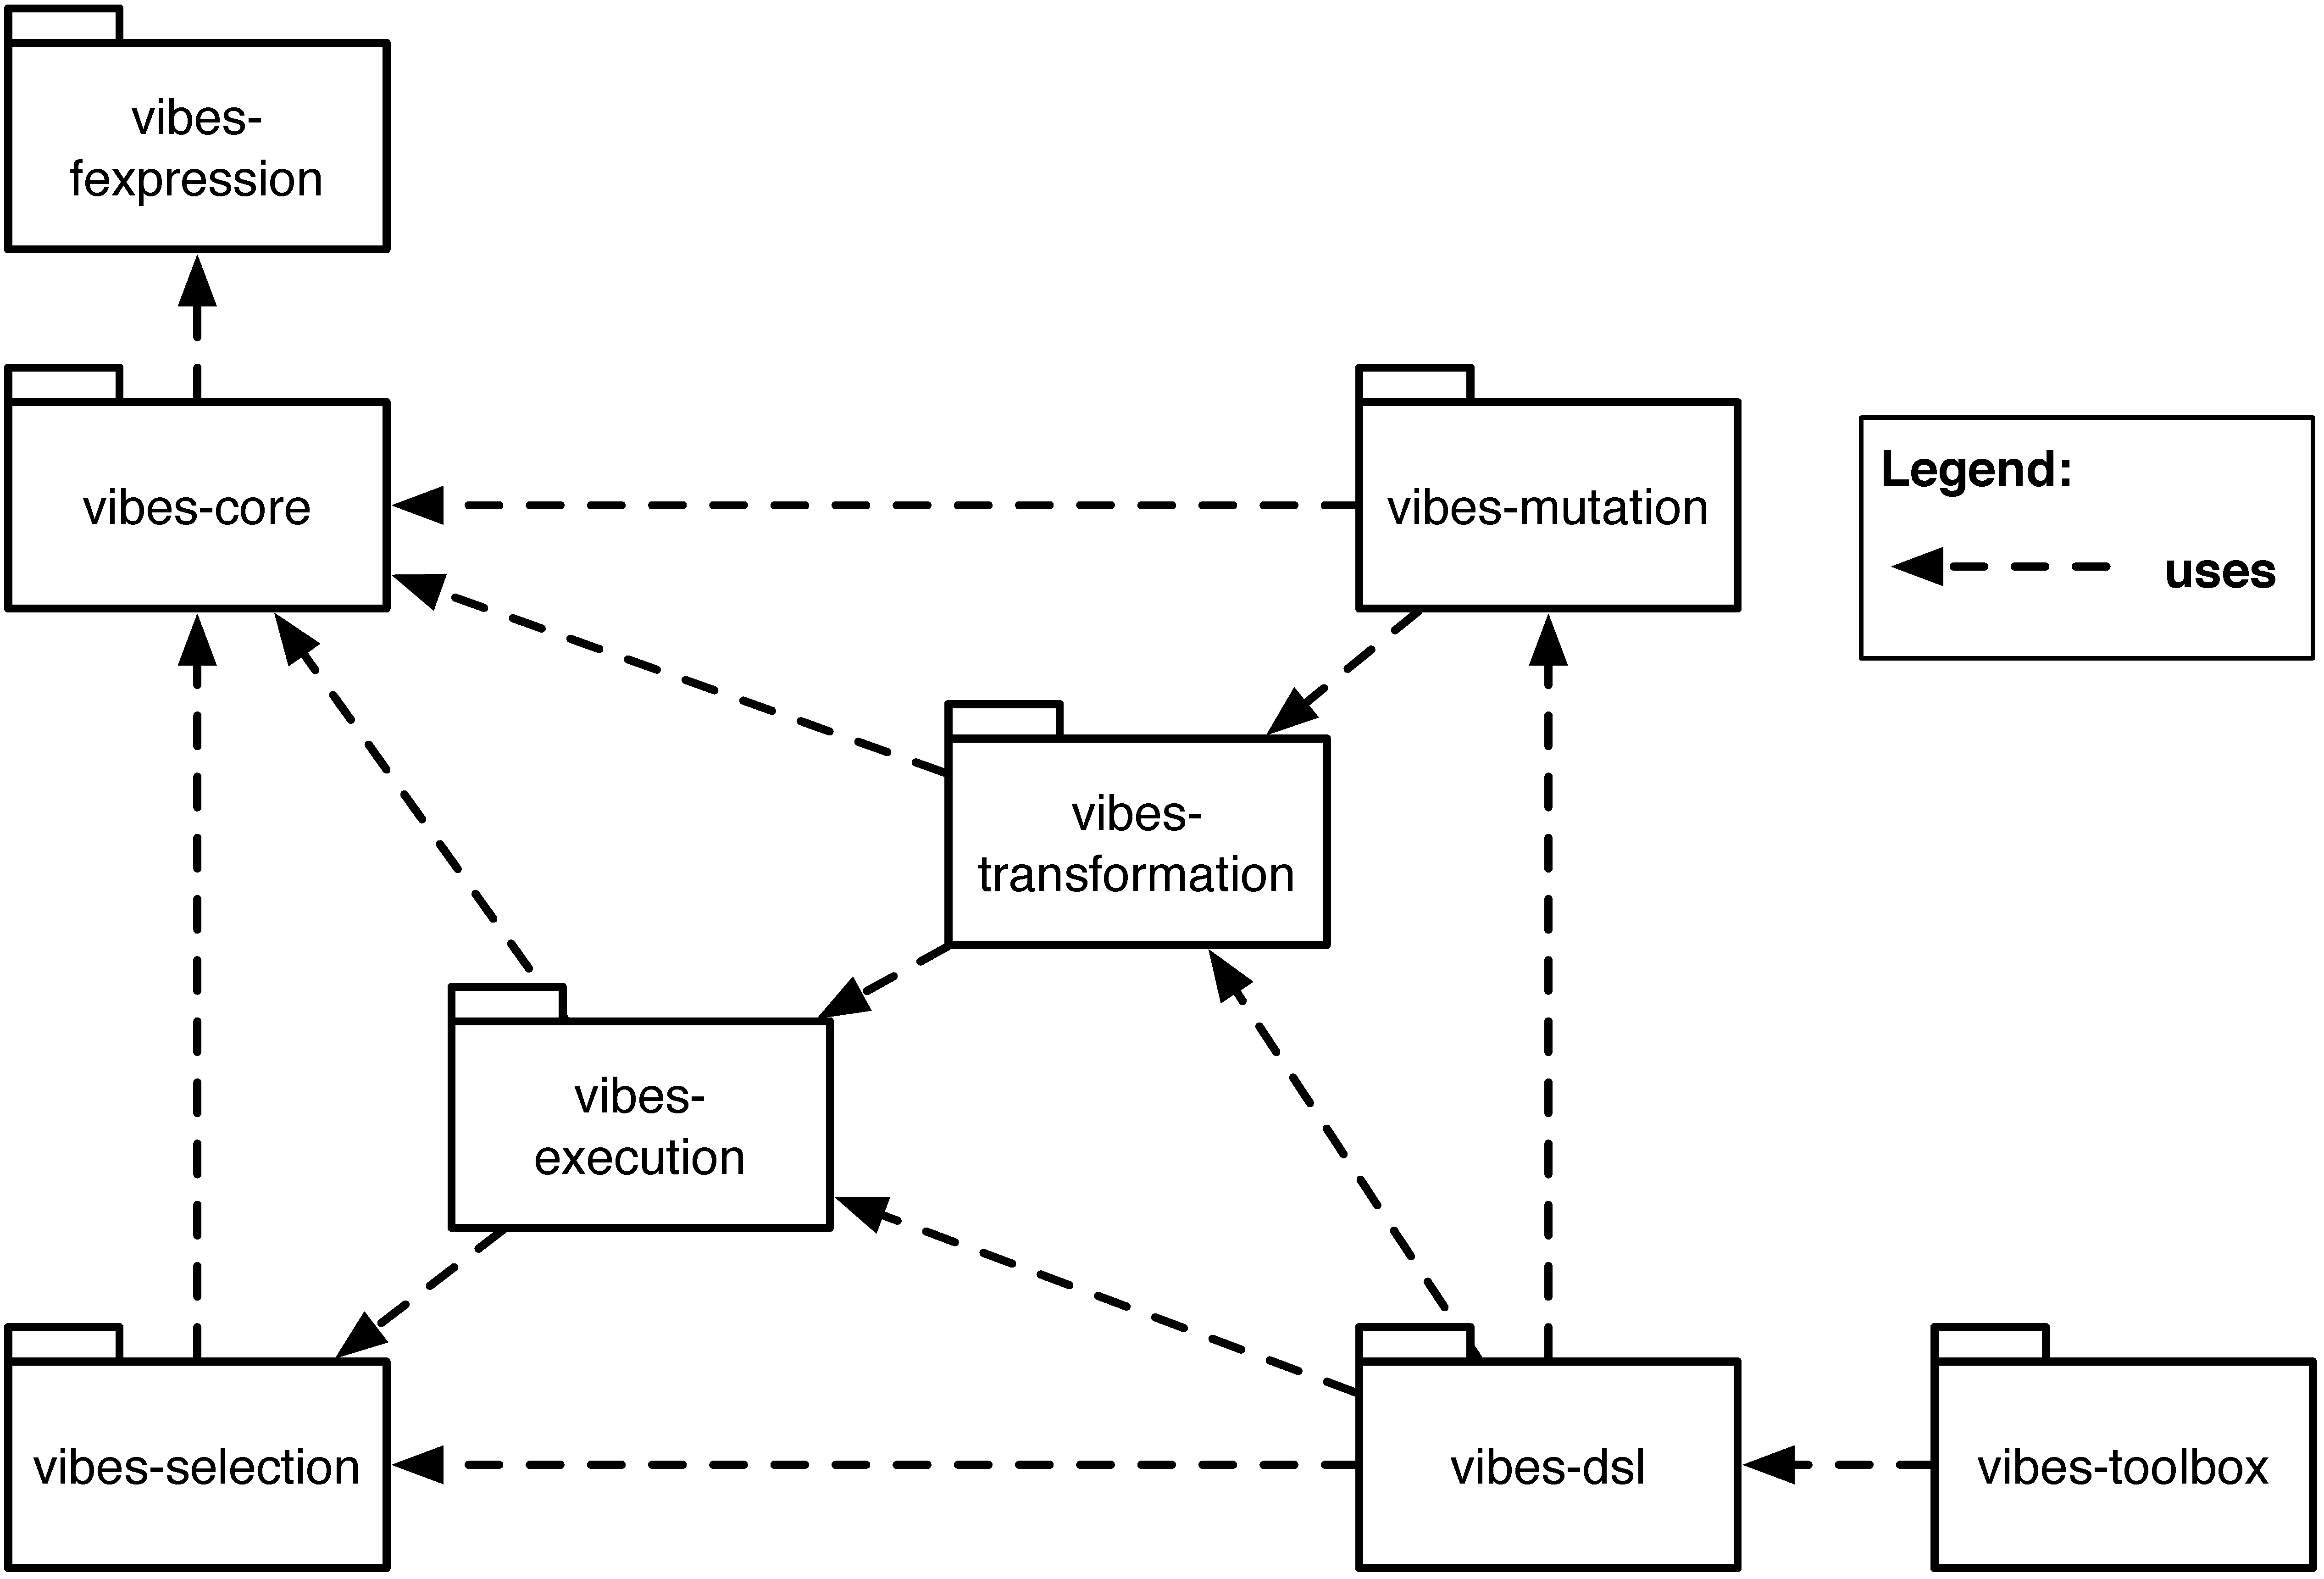
\includegraphics[width=110mm]{vibes-dependencies}
	\caption{\gls{VIBeS} modules dependency graph}
	\label{fig:vibesdependencies}
\end{figure} 

Maven allows to organise a project hierarchically. The root project is a \emph{Maven project}, while the sub-projects are \emph{Maven modules}. \gls{VIBeS}'s Maven project produces the artefact \texttt{be.unamur.info:vibes:1.1.6}, which is only a \gls{POM} without any associated Jar. \gls{VIBeS}'s project has several modules (with the same group identifier and version number as the parent project) regrouping different aspects of the framework. For instance, the modules \texttt{vibes-core} contains the core classes used to model \glspl{FTS}, module \texttt{vibes-selection} contains Java classes to perform test case selection from a \gls{FTS} model, \etc Figure \ref{fig:vibesdependencies} presents the different modules from \gls{VIBeS} and the dependencies between them: module \texttt{vibes-core} uses the \texttt{vibes-fexpression} modules that allows to represent and manipulate feature expressions; module \texttt{vibes-selection} presents an \gls{API} to select test cases from a transition system (\gls{FTS}, \gls{LTS}, or \gls{usage model}); module \texttt{vibes-execution} contains the \gls{API} to execute abstract test cases on the transition systems; \texttt{vibes-transformation} allows to transform, serialize, or deserialize the transition systems using different formalisms (\eg XML, DOT file, timbuk automata, \etc); module \texttt{vibes-mutation} contains the \gls{API} to perform mutation analysis; \texttt{vibes-dsl} encapsulates the different \gls{API} to present a unified Java DSL to perform the different testing activities using \gls{VIBeS}; and \texttt{vibes-toolbox} contains all the sub-modules that uses the Java DSL to implement toolboxes to perform particular tasks (\eg generate mutants). 

\begin{figure}
	\centering
	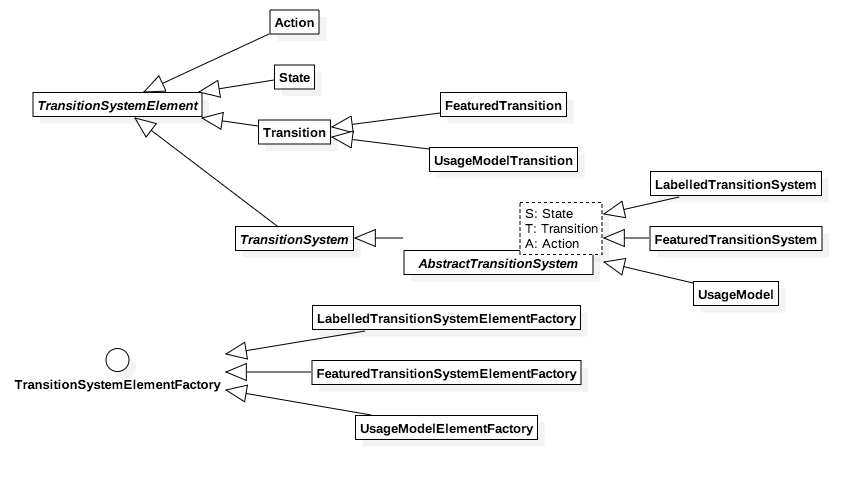
\includegraphics[width=\textwidth]{vibes-type-hierarchy}
	\caption{\gls{VIBeS} type hierarchy class diagram}
	\label{fig:vibestypehierarchy}
\end{figure} 

Classes from the \texttt{vibes-core} modules represent the transition systems used by \gls{VIBeS}. Figure \ref{fig:vibestypehierarchy} presents the class hierarchy of the different elements. Each element of a transitions system (actions, states, transitions, and the transition system itself) extends the \texttt{Tran\-si\-tion\-Sys\-tem\-Ele\-ment} class. Transitions are either simple transitions (\texttt{Transition} class) or transitions labelled by feature expression (\texttt{FeaturedTransition} class) or a probability (\texttt{UsageModelTransition} class). Transition systems (\texttt{Label\-led\-Tran\-sition\-System}, \texttt{Fea\-tu\-red\-Tran\-sit\-ion\-System}, and \texttt{Usage\-Mo\-del}) extends the \texttt{Ab\-stract\-Tran\-si\-tion\-System} class,  which is parametrized with the type of states, transitions, and actions used for this transition system (featured transitions for the \glspl{FTS} for instance). To manage the creation of the different elements of a transition system, a dedicated factory, extending \texttt{Tran\-si\-tion\-Sys\-tem\-Ele\-ment\-Facto\-ry}, is used.

Figure \ref{fig:vibescore} presents how transition systems are represented. A transition system (class \texttt{TransitionSystem}) is a collection of actions and states, with an initial state. Each state has incoming and outgoing transitions, and each transition is labelled with an action belonging to the same transition system. The default transition system implementation (class \texttt{AbstractTransitionSystem}) uses a factory to build the different states, actions, and transitions. This insures to respect the representation invariant of the class.

\begin{figure}
	\centering
	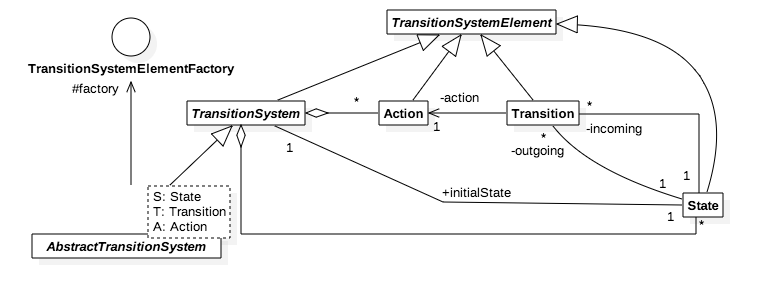
\includegraphics[width=\textwidth]{vibes-core}
	\caption{\gls{VIBeS} transition systems class diagram}
	\label{fig:vibescore}
\end{figure}


%%%%%%%%%%%%%%%%%%%%%%%%%%%%%%
\section{API usage}
%%%%%%%%%%%%%%%%%%%%%%%%%%%%%%

\label{sec:vibesusages}

The simplest way to use \gls{VIBeS} is to create a new Maven project and add a dependency to  \texttt{be.unamur.info:vibes-dsl:1.1.6}:
%
\begin{lstlisting}[language=XML,frame=single,numbers=none,morekeywords={dependency,groupId,artifactId,version}]
<dependency>
    <groupId>be.unamur.info</groupId>
    <artifactId>vibes-dsl</artifactId>
    <version>1.1.6</version>
</dependency>
\end{lstlisting}
This artefact contains an \gls{API} that encapsulates most of \gls{VIBeS} usages. The \texttt{vibes-dsl} module has been built following the same philosophy as the Apache Camel Java DSL\footnote{See \url{http://camel.apache.org}.} to chain method calls in order to facilitate the model definition, test case selection, mutation analysis, \etc

%------------------------------------
\subsection{Model definition}
%------------------------------------

Definition of a new \gls{FTS} is done by extending the \texttt{Featured\-Tran\-si\-tion\-Sys\-tem\-De\-fi\-ni\-tion} class  and implementing the abstract \texttt{define} method of that class. This method calls other inherited methods to define the initial state, states, actions, and transitions. For instance, the \gls{soda vending machine} \gls{FTS} from Section \ref{sec:casestudy:svm} is defined as:
%
\begin{lstlisting}[language=Java,frame=single,numbers=none]
public class SodaVendingMachineModel extends FeaturedTransitionSystemDefinition{
    
    private static final String[] S = new String[]{"s1", "s2", "s3", "s4", "s5", "s6", "s7", "s8", "s9"};

    @Override
    protected void define() {
        initial(S[0]); // Define the initial state

        from(S[0]).action("pay").fexpr("!f").to(S[1]);
        from(S[0]).action("free").fexpr("f").to(S[2]);
        
        from(S[1]).action("change").fexpr("!f").to(S[2]);
        from(S[2]).action("cancel").fexpr("c").to(S[3]);
        
        from(S[3]).action("return").fexpr("c").to(S[0]);
        from(S[3]).action("soda").fexpr("s").to(S[4]);
        from(S[3]).action("tea").fexpr("t").to(S[5]);
        
        from(S[4]).action("serveSoda").fexpr("s").to(S[6]);
        from(S[5]).action("serveTea").fexpr("t").to(S[6]);
        
        from(S[6]).action("take").fexpr("f").to(S[0]);
        from(S[6]).action("open").fexpr("!f").to(S[7]);
        
        from(S[7]).action("take").fexpr("!f").to(S[8]);
        from(S[8]).action("close").fexpr("!f").to(S[0]);
    }   
}
\end{lstlisting}
%
The model can be instantiated by calling the \texttt{getTransitionSystem} method:
%
\begin{lstlisting}[language=Java,frame=single,numbers=none]
FeaturedTransitionSystem svm = new SodaVendingMachineModel().getTransitionSystem();
\end{lstlisting}
%
Transitions may be tagged with an action or a feature expression. \Glspl{feature expression} must respect the following grammar:
%
\begin{lstlisting}[frame=single,numbers=none]
fexpression: 'true'
			| 'false'
			| featureName
			| '(' fexpression ')'
			| '!' fexpression
			| fexpression ('&&' | '||') fexpression ;

featureName: LETTER (LETTER | DIGIT)* ;

LETTER: 'A'..'Z' | 'a'..'z' | '_';
DIGIT: '0'..'9';
\end{lstlisting}
%
Feature names must begin by a letter, and may contain letters or digits. Operators have the following priority rules: negation ('\texttt{!}') takes precedence over conjunction ('\texttt{\&\&}') and disjunction ('\texttt{||}').

%------------------------------------
\subsection{Test suite selection}
%------------------------------------

Test suite selection may be done manually, or using one of the selection criterion defined in Chapter \ref{chap:coverage}. 

\paragraph{Manual test suite selection:}
%----------------------------------------

Manual selection is done by extending the \texttt{Test\-Set\-De\-fi\-ni\-tion} class. As for the model definition, the \texttt{define} method has to be implemented and call inherited methods to define the test cases:
%
\begin{lstlisting}[language=Java,frame=single,numbers=none]
public class ManualTestSuite extends TestSuiteDefinition{

    @Override
    protected void define() {
        id("testRefund").action("pay").action("change").action("cancel").action("return").end();
        id("testFreeTea").action("free", "tea", "serveTea", "take");
        id("testNoFreeSoda").action("pay", "change").action("soda", "serveSoda").action("open", "take", "close");
    }
}
\end{lstlisting}
%
Actions may be added one by one or by groups in the same \texttt{action} method call. The test suite is instantiated using the \texttt{getTestSet} method:
%
\begin{lstlisting}[language=Java,frame=single,numbers=none]
TestSet testSuite = new ManualTestSuite().getTestSet();
\end{lstlisting}
%


\paragraph{Random selection:}
%----------------------------------------

Random test suite selection selects a defined number of test cases by random walks in \gls{FTS}. This requires the \gls{feature model} of the \gls{FTS} from which test cases are selected to ensure that selected test cases are positive abstract test cases. This feature model is encapsulated in a constraint solver (Sat4j\footnote{See \url{http://www.sat4j.org}.} for instance), accessed trough a facade that implements the \texttt{SolverFacade} interface. To load the feature model, one may use a feature expression (a \gls{CNF} boolean expression representing the feature model) or load it from a DIMACS CNF file. In the following example, we load the feature model from a DIMACS CNF file:
%
\begin{lstlisting}[language=Java,frame=single,numbers=none]
// Feature model loading
DimacsModel featureModel = DimacsModel.createFromDimacsFile("svm.dimacs");
SolverFacade solver = new Sat4JSolverFacade(featureModel);  

// Random test suite selection
TestSet randomSuite = randomSelection(svm, solver);
\end{lstlisting}
%


\paragraph{All-states selection:}
%----------------------------------------

Selection of a test suite satisfying the all-state criterion is done by importing the \texttt{allStatesSelection} static method from the \texttt{AllStates} class:
%
\begin{lstlisting}[language=Java,frame=single,numbers=none]
// Feature model loading
DimacsModel featureModel = DimacsModel.createFromDimacsFile("svm.splot.dimacs");
SolverFacade solver = new Sat4JSolverFacade(featureModel);  

// All-states test suite selection
TestSet allStatesSuite = allStatesSelection(svm, solver);
\end{lstlisting}
%

\paragraph{Dissimilarity-driven selection:}
%----------------------------------------

Test suite selection using a dissimilarity heuristic is done using the \texttt{Dissimilar} class. The heuristic may be configured using the following methods:
%
\begin{lstlisting}[language=Java,frame=single,numbers=none]
// Feature model loading
DimacsModel featureModel = DimacsModel.createFromDimacsFile("svm.splot.dimacs");
SolverFacade solver = new Sat4JSolverFacade(featureModel);  

// Dissimilar selection
from(svm, solver)
	.during(30000) // specify duration
	// specify local or global distance and how to compute dissimilarity
	.withLocalMaxDistance(ftsDissimilarity(solver, levenshtein(), avg()))
	// Specify the number of test cases
	.generate(5);
\end{lstlisting}
%
Duration specifies how long the algorithm will run, using a local (\texttt{with\-Local\-Max\-Dis\-tance}) or global (\texttt{with\-Glo\-bal\-Max\-Dis\-tance}) distance computation. The distance itself is defined using one of the static methods that works on the actions alone (\texttt{hamming}, \texttt{jaccard}, \texttt{dice}, \texttt{antidice}, or \texttt{levenshtein}), or in combination with product distance (\texttt{fts\-Dis\-si\-mi\-la\-ri\-ty}), using a binary operator (\texttt{avg}, \texttt{mul}, or any other \texttt{Bi\-na\-ry\-Ope\-ra\-tor} object).

\paragraph{Usage-based selection:}
%----------------------------------------

Usage based selection is more complex. First, it requires to select a set of test cases in the \gls{usage model} using \texttt{Boun\-ded\-Pro\-ba\-bi\-li\-ty\-Ge\-ne\-ra\-tor} class. Those test cases are then executed on the \gls{FTS} that is pruned to keep only transitions activated by at least one test case. This is done using the \texttt{Prun\-ning.pru\-ne} method. Complete usage-based test suite selection is not yet encapsulated in \texttt{vibes-dsl}. This is part of our future work.

%-------------------------------------------------------
\subsection{Saving and loading models}
%-------------------------------------------------------

Models may be saved in XML format using the \texttt{Tran\-si\-tion\-Sy\-stem\-Xml\-Prin\-ter} class. To load a model from an XML file, one may use the \texttt{Tran\-si\-tion\-Sys\-tem\-Xml\-Loa\-ders} class:
%
\begin{lstlisting}[language=Java,frame=single,numbers=none]
// Load model
FeaturedTransitionSystem svm = loadFeaturedTransitionSystem("svm.xml");

// Save model
print(svm, "svm.xml");
\end{lstlisting}
%
The XML model of the soda vending machine is the following:
%
\begin{lstlisting}[language=XML,frame=single,numbers=none]
<?xml version="1.0" encoding="utf-8"?>
<fts xmlns="http://www.unamur.be/xml/fts/" xmlns:xsi="http://www.w3.org/2001/XMLSchema-instance">
  <start>state1</start>
  <states>
    <state id="state1">
      <transition action="pay" fexpression="!FreeDrinks" target="state2"/>
      <transition action="free" fexpression="FreeDrinks" target="state3"/>
    </state>
    <state id="state2">
      <transition action="change" fexpression="!FreeDrinks" target="state3"/>
    </state>
    ...
  </states>
</fts>
\end{lstlisting}

%-------------------------------------------------------
\subsection{Performing mutation analysis}
%-------------------------------------------------------

Mutation analysis consist of mutants generation (in an enumerative or \gls{FMM} approach) and mutants execution. Those analysis are done at the product level (on \glspl{LTS}), mutation analysis for \glspl{FTS} is part of our future works. 

\paragraph{Mutation operators configuration:}
%---------------------------------------------

Operators may be configured using the \texttt{Mu\-ta\-gen} class. This is useful to define the selection strategy of the elements to mutate. For instance, one can create a state missing (SMI) operator that will only remove particular states (chosen randomly):
%
\begin{lstlisting}[language=Java,frame=single,numbers=none]
MutationOperator op = Mutagen.stateMissing(svm)
	.stateSelectionStrategy(svm.getState("s4"), svm.getState("s8"), svm.getState("s9"))
	.done();
\end{lstlisting}
%
One may also configure a set of operators using an XML configuration file:
%
\begin{lstlisting}[language=XML,frame=single,numbers=none]
<?xml version="1.0" encoding="utf-8"?>
<config>
  <!-- Default mutant size (may be redefined) -->
  <mutantsSize>200</mutantsSize>
  <!-- Default selection strategies (may be redefined) -->
  <actionSelection>
    be.unamur.transitionsystem.test.mutation.RandomSelectionStrategy
  </actionSelection>
  <stateSelection>
    be.unamur.transitionsystem.test.mutation.RandomSelectionStrategy
  </stateSelection>
  <transitionSelection>
    be.unamur.transitionsystem.test.mutation.RandomSelectionStrategy
  </transitionSelection>
  <!-- Default uniqueness of each mutant (may be redefined) -->
  <unique>true</unique>
  <!-- Operators -->
  <operators>
    <operator>
      <class>be.unamur.transitionsystem.test.mutation.ActionExchange</class>
    </operator>
    ...
    <operator>
      <class>be.unamur.transitionsystem.test.mutation.WrongInitialState</class>
      <mutantsSize>100</mutantsSize>
      <actionSelection>be.dummy.MyActStrategy</actionSelection>
      <stateSelection>be.dummy.MyStStrategy</stateSelection>
      <transitionSelection>be.dummy.MyTrStrategy</transitionSelection>
      <unique>false</unique>
    </operator>
  </operators>
</config>
\end{lstlisting}
%
Default configuration (selection strategy, number of mutants to generate, uniqueness on mutant based on the selected operands of the operator) may be redefined for each mutation operator.

\paragraph{Mutants generation (enumerative approach):}
%-------------------------------------------------------

Mutants may be generated enumeratively: each mutant is generated in a new XML file. For instance:
%
\begin{lstlisting}[language=Java,frame=single,numbers=none]
LabelledTransitionSystem lts = loadLabelledTransitionSystem("product.xml");
configure("operatorsConfig.xml")
	.outputDir("mutants/") // Generates mutants in the given folder
	.mutate(lts);
\end{lstlisting}
%

\paragraph{Mutants generation (\gls{FMM} approach):}
%-------------------------------------------------------

One can also generate a \gls{FMM} and save it in an XML and a \gls{TVL} files :
%
\begin{lstlisting}[language=Java,frame=single,numbers=none]
LabelledTransitionSystem lts = loadLabelledTransitionSystem("product.xml");
FeaturedMutantsModel fmm = configure("operatorsConfig.xml")
	.ftsMutant("fmm.fts") // Generates FMM's FTS with given name
	.tvlMutant("fmm.tvl") // Generates FMM's FD in TVL format
	.mutate(lts);
\end{lstlisting}
%

\paragraph{Mutants execution:}
%------------------------------

Finally, execution of a test suite on the \gls{FMM} is done using the \texttt{get\-Alive\-Mu\-tants} static method of the \texttt{Fea\-tu\-red\-Mu\-tants\-Mo\-dels} class:
%
\begin{lstlisting}[language=Java,frame=single,numbers=none]
FExpression alive = getAliveMutants(testSuite.get(0), fmm);
solver.addConstraint(alive);
Iterator<Configuration> solutions = solver.getSolutions();
while(solutions.hasNext()) {
	System.out.println(solutions.next());
}
\end{lstlisting}
%

%------------------------------------
\subsection{\gls{VIBeS} toolboxes}
%------------------------------------

\gls{VIBeS} architecture in Maven modules allows to do rapid prototyping. Module \texttt{vibes-dsl} encapsulates the common operations performed during the testing activities to reduce as much as possible custom developments. Beside \texttt{vibes-dsl} module,  \gls{VIBeS} also comes with a set of toolboxes. Each of those toolbox is a executable Jar file with a command line interface that may be used to perform standard tasks. The existing toolboxes are:
\begin{itemize}
\item \texttt{toolbox-model-statistics}: to print statistics about a transition system;
\item \texttt{toolbox-testcase-generation}: to select test suites using various criteria;
\item \texttt{toolbox-transformation}: to transform an XML transition system to other formats (\eg Graphviz DOT);
\item \texttt{toolbox-products-analyze}: to print the number of products for a given feature model and a given feature expression;
\item \texttt{toolbox-mutant-generation}: to generate mutants (enumeratively or using a \gls{FMM});
\item \texttt{toolbox-fmm-execution}: to execute test cases on a \gls{FMM};
\item \texttt{toolbox-mutation-equivalence}: to detect equivalent mutants using simulation or automata language equivalence;
\item \texttt{toolbox-mutant-sampling}: to sample a set of mutants (from different orders) from a given \gls{FMM}.
\end{itemize}


%%%%%%%%%%%%%%%%%%%%%%%%%%%%%%%%%%%%
\section{Wrap up}
%%%%%%%%%%%%%%%%%%%%%%%%%%%%%%%%%%%%

\label{sec:vibesperspectives}

In this chapter, we present \gls{VIBeS}, the implementation of our testing framework. We use \gls{VIBeS} to perform various testing activities, including model definition, test suite selection, and mutation analysis. 

\gls{VIBeS} is built as a Maven project with several modules. Each module is dedicated to one particular aspect of the testing activities. Test engineers may use \gls{VIBeS} by accessing the API of the different modules, or by using the Java DSL that encapsulates API calls and simplifies usages. 

This modular architecture allows to perform rapid prototyping while allowing adhoc developments for specific needs. We choose to use Java as the interface language for the test engineer rather than a dedicated DSL or modelling language. This avoids to switch between syntaxes and, we assume, lowers the learning curve for new users. This idea stems from industrial practices (like Apache Camel\footnote{See \url{http://camel.apache.org}.}) and seems to be confirmed by other trending behavioural testing tools (like Cucumber \cite{cucumber} where, except for the behavioural description of the system, all elements are defined in Java).

%Future work includes a refactoring and refinement of \gls{VIBeS} Java DSL to standardize names and encapsulate calls to the most recent parts of the API (like mutant equivalence detection and usage-based test suite selection). Finally, performance of the different test suite selection algorithms and mutant execution algorithms may be improved in order to reduce execution time and memory consumption.



\chapter{Test case concretization using AbsCon}
\chaptermark{AbsCon}
\label{chap:concretization}

Test definition and execution is an essential but time-consuming task during system development. To speed up the process, model-based testing and other related approaches propose to select abstract test cases and to automatically concretize them, based on mapping information provided by the test engineer. This mapping may take one of the following forms \cite{Utting2007}:
\begin{inparaenum}[(i)]
\item an adapter which interprets the actions and assertions of the abstract test case and execute them on the SUT;
\item a transformation from the abstract test cases to code executable directly on the SUT; or
\item a mixture of the above two.
\end{inparaenum}
In this last case, an \gls{abstract test case} is transformed into executable code which uses an intermediate adapter (like an intermediate library for instance) to bridge the gap between the test case and the \gls{SUT}. 

In this chapter, we describe the \acrfull{AbsCon} developed by Jeremy Vanhecke \cite{Vanhecke2016} during his master thesis, we co-supervised with Dr. Gilles Perrouin and Prof. Patrick Heymans. AbsCon is defined as a QTaste \cite{qtaste} plugin, an open-source industrial data-driven test case definition and execution environment, used to perform black-box testing on various kinds of systems. QTaste abstracts the SUT's interface by using an adapter called \emph{test API}, test cases are written in Python where the operations on and the readings from the SUT's interface are encapsulated into calls to the test API dedicated to the kind of the SUT. 

For instance, to test a Web-application, QTaste encapsulates the access to the elements of the Web page in a Web test API which is responsible to perform the effective Selenium (a popular Web browser automation tool \cite{selenium}) calls. After considering different options, we chose to define AbsCon as a QTaste plugin for the following reasons:
\begin{inparaenum}[(i)]
	\item QTaste is an open source industrial tool, used to test various kinds of systems, from Web-applications to mobile applications and even cyber-physical systems \cite{Doucet2014}, thanks to its test API adaptation mechanism;
	\item plugin development is already included in QTaste and this architecture was suggested by a QTaste developer;
	\item the inital goal of AbsCon was to concretize abstract test cases selected by \gls{VIBeS} using additional mapping information. To this end, abstract test cases are defined in AbsCon using an XML file, where each test case is a sequence of actions and assertions on the SUT. But this definition is not specific to VIBeS, it also allows QTaste test engineers to define test cases in a more abstract and systematic fashion (rather than directly Python scripts), as long as they follow the same pattern (\ie sequences of assertions and actions).
\end{inparaenum}

The remainder of this chapter is as follows: Section \ref{sec:abscon:qtaste} gives a general description of the QTaste environment, Section \ref{sec:abscon:abscon} describes AbsCon's \gls{concretization} process as well as the required mapping information, Section \ref{sec:abscon:architecture} presents AbsCon's implementation, advantages and limitations are discussed in Section \ref{sec:abscon:discussion}, Section \ref{sec:abscon:relatedwork} discusses related work. Finally, Section \ref{sec:abscon:conclusion} wraps up the chapter and presents some perspectives.


%%%%%%%%%%%%%%%%%%%%%%%%%%%%%%%%%%%%%%%%%%%%%%
\section{Test automation using QTaste}
%%%%%%%%%%%%%%%%%%%%%%%%%%%%%%%%%%%%%%%%%%%%%%

\label{sec:abscon:qtaste}

The \acrfull{QTaste} \cite{qtaste} is an open source functional and non-functional black-box test environment developed in Java and Python. It has been originally developed by Qspin Experts\footnote{\url{http://www.qspin.be}} in order to automate testing process of medical cyber-physical systems developed by IBA\footnote{\url{https://iba-worldwide.com}} and used for proton therapy. 
Since its inception, QTaste has been extended to support different kinds of SUTs, like Web-applications, mobile applications, or more classical desktop applications \cite{Doucet2014}. It is released as an open source project on GitHub under GNU GPL 3.0 license \cite{qtaste}. 

%------------------------------------------------
\subsection{Overview of the QTaste environment}
%------------------------------------------------

QTaste follows the data-driven testing philosophy \cite{Williams2007}: data used by the tests are externalized in order to allow test cases parametrization. Each test case is written in Python and describes a sequence of steps, \ie \emph{operations} executed by the SUT or \emph{verifications} of the outputs produced by this SUT, using the given data as input. For instance, when testing a form which values are recorded in a database, one test case fills the form with the given data and check that the values are effectively recorded in the database. This test case is repeated with different values (\eg positive, null, and negative values for numeric fields) specified in a separate CSV file and automatically executed by QTaste on the SUT. 


\paragraph{QTaste adapter mechanism:}
%------------------------------------

QTaste provides \textit{test APIs} which communicate with the \gls{SUT} and manage the  operations executions and/or SUT's outputs reading. Each test API consists in a Java interface, defining the operations and information accessible by the test cases, and a Java implementation of this interface which manages communication with the SUT. 
This mechanism allows QTaste to test a large variety of systems: Web-applications using a Selenium-based test API, hardware components with dedicated API, or any other kind of system for which a test API may be developed. The test API, together with the configuration of the SUT instance is called a \emph{Testbed}: this mechanism allows to write test cases independently from the execution environment, using only test (and standard Python) API(s). 
Once all the test cases have been executed, QTaste generates a summary report, with the number of success and fails, the Testbed used, for each test case, the CSV lines used, \etc


\paragraph{Example:}
%------------------------------------

\begin{lstlisting}[language=Python,
float,
label=lst:abscon:testcase,
caption={Google search test case}]
from qtaste import *

api = testAPI.getSelenium(INSTANCE_ID='Google')(*@\label{lst:abscon:testcase:selenium}@*)

def init():(*@\label{lst:abscon:testcase:init}@*)
	api.openBrowser(testData.getValue("BROWSER"))(*@\label{lst:abscon:testcase:openbrowser}@*)
	api.windowMaximize()
	api.open("https://www.google.be/") (*@\label{lst:abscon:testcase:openurl}@*)
	api.waitForPageToLoad("15000") 
	if api.getTitle() != "Google": (*@\label{lst:abscon:testcase:checktitle}\label{lst:abscon:testcase:gettitle}@*)
		testAPI.stopTest(Status.FAIL)
    
def searchAndClick():(*@\label{lst:abscon:testcase:searchandclick}@*)
	api.type("id=lst-ib", testData.getValue("SEARCHVALUE"))(*@\label{lst:abscon:testcase:type}@*)  
	api.clickAt("name=btnK", "0.0" )(*@\label{lst:abscon:testcase:click1}@*)
	api.waitForPageToLoad("15000")
	api.click("link=" + testData.getValue("LINKTOCLICK"))(*@\label{lst:abscon:testcase:click2}@*)
	if api.getTitle() != testData.getValue("LINKTITLE"): (*@\label{lst:abscon:testcase:checklinktitle}@*)
		testAPI.stopTest(Status.FAIL)
		
def exit():(*@\label{lst:abscon:testcase:exit}@*)
	api.stop()(*@\label{lst:abscon:testcase:stopbrowser}@*)

doStep(init)(*@\label{lst:abscon:testcase:dostep1}@*)
doStep(searchAndClick)(*@\label{lst:abscon:testcase:dostep2}@*)
doStep(exit)(*@\label{lst:abscon:testcase:dostep3}@*)
\end{lstlisting}

Listing \ref{lst:abscon:testcase} presents a (simplified) test case for the Google search engine that is executed for each line of the external CSV file. It launches a Web browser and connects to the Google search website, fills the search field with a string, and click on a specified link. 
Line \ref{lst:abscon:testcase:selenium} creates a Selenium instance test API, which manages the connection to the browser; 
lines \ref{lst:abscon:testcase:init}, \ref{lst:abscon:testcase:searchandclick} and \ref{lst:abscon:testcase:exit} declare the steps of this test case, called at lines \ref{lst:abscon:testcase:dostep1}, \ref{lst:abscon:testcase:dostep2}, and \ref{lst:abscon:testcase:dostep3}; 
explanations about each step is given as a comment in Python format (not shown here) and is used during the generation of the test reports.
At each step, the test API instance is used to manipulate the browser user interface (lines \ref{lst:abscon:testcase:openbrowser} to \ref{lst:abscon:testcase:gettitle}, \ref{lst:abscon:testcase:type} to \ref{lst:abscon:testcase:checklinktitle}, and \ref{lst:abscon:testcase:stopbrowser}) according to the data provided in the external CSV file (identified by column names at lines \ref{lst:abscon:testcase:openbrowser}, \ref{lst:abscon:testcase:type}, \ref{lst:abscon:testcase:click2}, and \ref{lst:abscon:testcase:checklinktitle}). 
Finally, each step may check assertions on the outputs of the browser to validate the execution (lines \ref{lst:abscon:testcase:checktitle} and \ref{lst:abscon:testcase:checklinktitle}).


%---------------------------------------
\subsection{Advantages and limitations}
%---------------------------------------

The main advantage of QTaste is the test API mechanism, allowing test cases to manipulate a large variety of SUTs using a general purpose programming language: Python. Expressing test cases using a general purpose and popular programming language like Python benefits from the large number of available Python libraries. This can be very handful when writing test cases in order to perform more complex operations or access external resources. The environment provides extensibility mechanisms to the test engineers in order to write dedicated adapters between QTaste and SUTs, and describes the usage of those adapters in a test API. Coupled to the externalisation of data and SUT's configuration, it improves test cases \emph{reusability} and \emph{automation} of the test process \cite{Utting2007}. 

As it works as a black-box test environment, QTaste access the SUT through its interface, manipulated by the test cases trough the test API. This means that whenever the interface and/or the test API evolve, all the test cases using this interface and/or modified test API are impacted, increasing \emph{maintenance cost} \cite{Utting2007}. AbsCon provides an additional abstraction layer separating the different concerns thus reducing maintenance costs when combined with abstract test cases as presented in the next section.   


%%%%%%%%%%%%%%%%%%%%%%%%%%%%%%%%%%%%%%%%%%%%%%%%%%%%%%%%
\section{Test cases concretization}
%%%%%%%%%%%%%%%%%%%%%%%%%%%%%%%%%%%%%%%%%%%%%%%%%%%%%%%%

\label{sec:abscon:abscon}

\begin{figure}
	\centering
	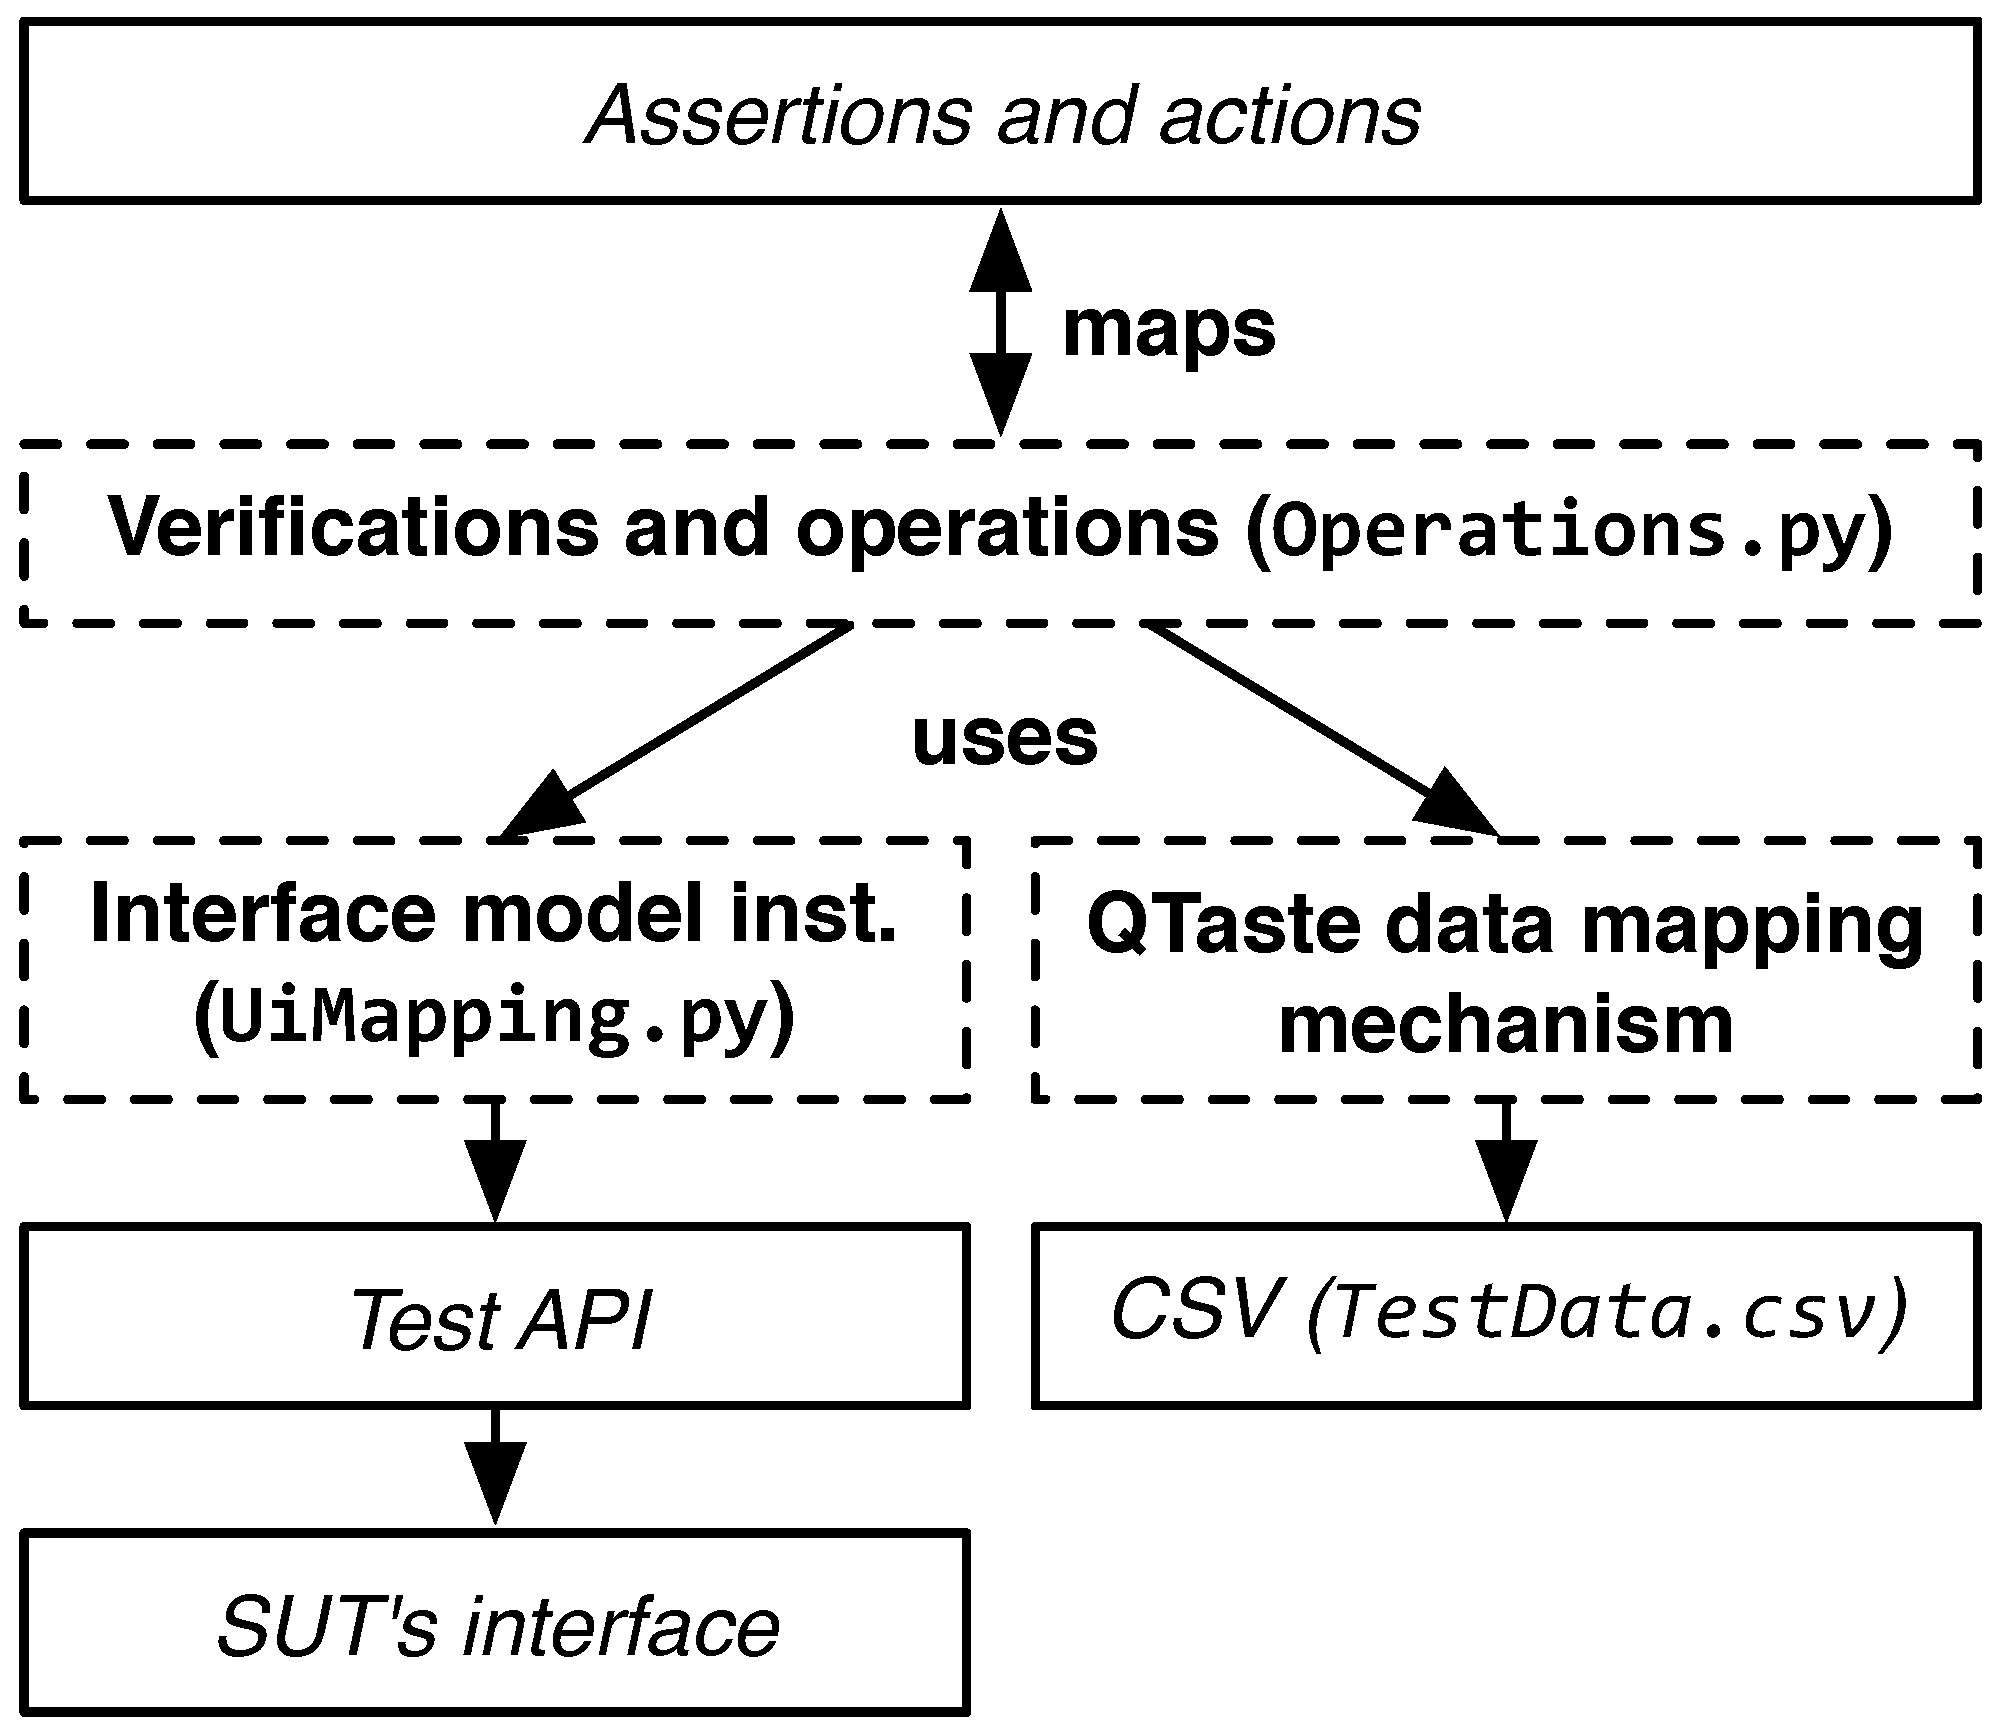
\includegraphics[width=0.33\textwidth]{abscon-mappings}
	\caption{Mappings in AbsCon}
	\label{fig:abscon:mappings}
\end{figure}

\gls{AbsCon} was originally developed to support \gls{abstract test case} \gls{concretization} \cite{Vanhecke2016}. In AbsCon, an abstract test case is a sequence of abstract \emph{assertions} and \emph{actions}, usually automatically derived by a model-based testing tool \cite{Utting2007}: VIBeS in this case \cite{vibes}. To bridge the gap between VIBeS and AbsCon, abstract test cases produced by VIBeS are enriched with the intermediate states (representing assertions on the system's state) visited when executing the abstract test case. This modification is coherent with our assumption that the behavioural model used to select  abstract test cases is deterministic.
 
The concretization process translates the abstract test case into a (concrete) test case executable by  QTaste: (resp.) \emph{assertions} and \emph{actions} are \emph{mapped} to (resp.) \emph{verifications} and \emph{sequences of operations} manipulating the SUT through the test API. The most common way to perform this task is to give, for each assertion and each action, the corresponding Python code. It allows to improve the reusability and automation, while decreasing the maintenance costs (each assertion or action is defined only once in the mapping). 

However, access to the SUT's interface elements remains hardcoded in the different test cases (\eg lines \ref{lst:abscon:testcase:gettitle} or \ref{lst:abscon:testcase:click1} in Listing \ref{lst:abscon:testcase}). This may raise one or more  issues:
\begin{enumerate}
	\item element of the SUT's interface are accessed using test API methods, requiring to know and provide at each method call the \emph{access method}  (\eg using the element's \texttt{id} or \texttt{name} or at lines \ref{lst:abscon:testcase:type} and \ref{lst:abscon:testcase:click1} in Listing \ref{lst:abscon:testcase}) and the \emph{access value} (\eg \texttt{lst-ib} at line \ref{lst:abscon:testcase:type} and \texttt{btnK} at line \ref{lst:abscon:testcase:click1} in Listing \ref{lst:abscon:testcase});
	\item besides being cumbersome when writing test cases, requiring access method and value in each method calls may also raise  problems, as not all elements of test API may be called on all elements of the SUT's interface (\eg for a Web-application, it is only possible to type text in text fields or in text areas), which will only be checked when running the test case;
	\item as previously, when an interface or test API element is updated, all the actions and/or assertions using this element are impacted, requiring to update the mapping in different places and thus increasing the maintenance cost (with a more limited magnitude).
\end{enumerate}

To mitigate those issues, we divide the mapping in AbsCon in three elements, as illustrated by the dashed boxes in Figure \ref{fig:abscon:mappings}: a SUT's interface elements mapping trough a \emph{model instance} of this interface; a \emph{data mapping}; and an \emph{assertions and actions mapping}, giving for each (resp.) assertion/action the (resp.) verifications/operations to perform on the SUT. The verifications and operations on the SUT are defined as Python functions that will use the interface model instance, using the methods of the different elements, and the external data. The external data are recorded in a CSV file and managed using QTaste's dedicated mechanism. The interface model, \ie a set of Python classes, uses one or more test APIs in order to execute the operations and retrieve information on/from the SUT. 

\begin{lstlisting}[language=XML,
float,
label=lst:abscon:xmltestcase,
caption={Google instant search test cases in AbsCon XML format}]
<?xml version="1.0" encoding="UTF-8"?>
<realisation id="Google testing">
	<uimodel>web</uimodel>  (*@\label{lst:abscon:xmltestcase:uimodel}@*)	
	<uimapping>UiMappings.py</uimapping> (*@\label{lst:abscon:xmltestcase:uimapping}@*)
	<operations>Operations.py</operations> (*@\label{lst:abscon:xmltestcase:operations}@*)
	<datas>TestData.csv</datas>  (*@\label{lst:abscon:xmltestcase:datas}@*)
	<tests>
		<test> (*@\label{lst:abscon:xmltestcase:testcase1}@*)
			<action>start</action>
			<action>goHomePage</action>
			<assert>onHomePage</assert>
			<action>inputSearchString</action>
			<assert>searchResultsPrinted</assert>
			<action>clickLink</action>
			<assert>pageLoaded</assert>
			<action>exit</action>
		</test> (*@\label{lst:abscon:xmltestcase:endtestcase1}@*)
	...
	</tests>
</realisation>
\end{lstlisting}

The model of the interface and the assertion/actions mapping is detailed in the following sections. To illustrate those different mappings, we will use Google instant search as SUT and consider the following test cases:
%
\begin{enumerate}
\item \label{testcase1} open Google search website, enter a keyword, see that search results are printed, click on a link, and check that the website is loaded;
\item \label{testcase2} open Google search website, enter a keyword, see that search results are printed, deactivate the instant search in the parameters and validate, go back to the main page, and check that search results are not printed when a keyword is entered;
\item \label{testcase3} open Google search website, enter a keyword, see that search results are printed, deactivate the instant search in the parameters and cancel, go back to the main page, and check that search results are printed when a keyword is entered.
\end{enumerate}
%
Test case (\ref{testcase1}) checks the common usage of Google instant search, test case (\ref{testcase2}) checks that, when the instant search is deactivated in the parameters options, the instant search is not performed, and test case \ref{testcase3} checks that when instant search is deactivated but the change is cancelled in the parameters options, instant search is still active. 
Test cases are defined in XML format as a sequence of assertions and actions: lines \ref{lst:abscon:xmltestcase:testcase1} to \ref{lst:abscon:xmltestcase:endtestcase1} in Listing \ref{lst:abscon:xmltestcase} gives test case \ref{testcase1} definition (other test cases are omitted). Additional information are the SUT's interface model to use (line \ref{lst:abscon:xmltestcase:uimodel}), the path to the Python file defining the instance of this model for the Google instant search interface (line \ref{lst:abscon:xmltestcase:uimapping}), the path to the Python file defining the operations mapping (line \ref{lst:abscon:xmltestcase:operations}), and the path to the external CSV data file (line \ref{lst:abscon:xmltestcase:datas}).

%----------------------------------
\subsection{SUT's interface model}
%----------------------------------

\begin{figure}
	\centering
	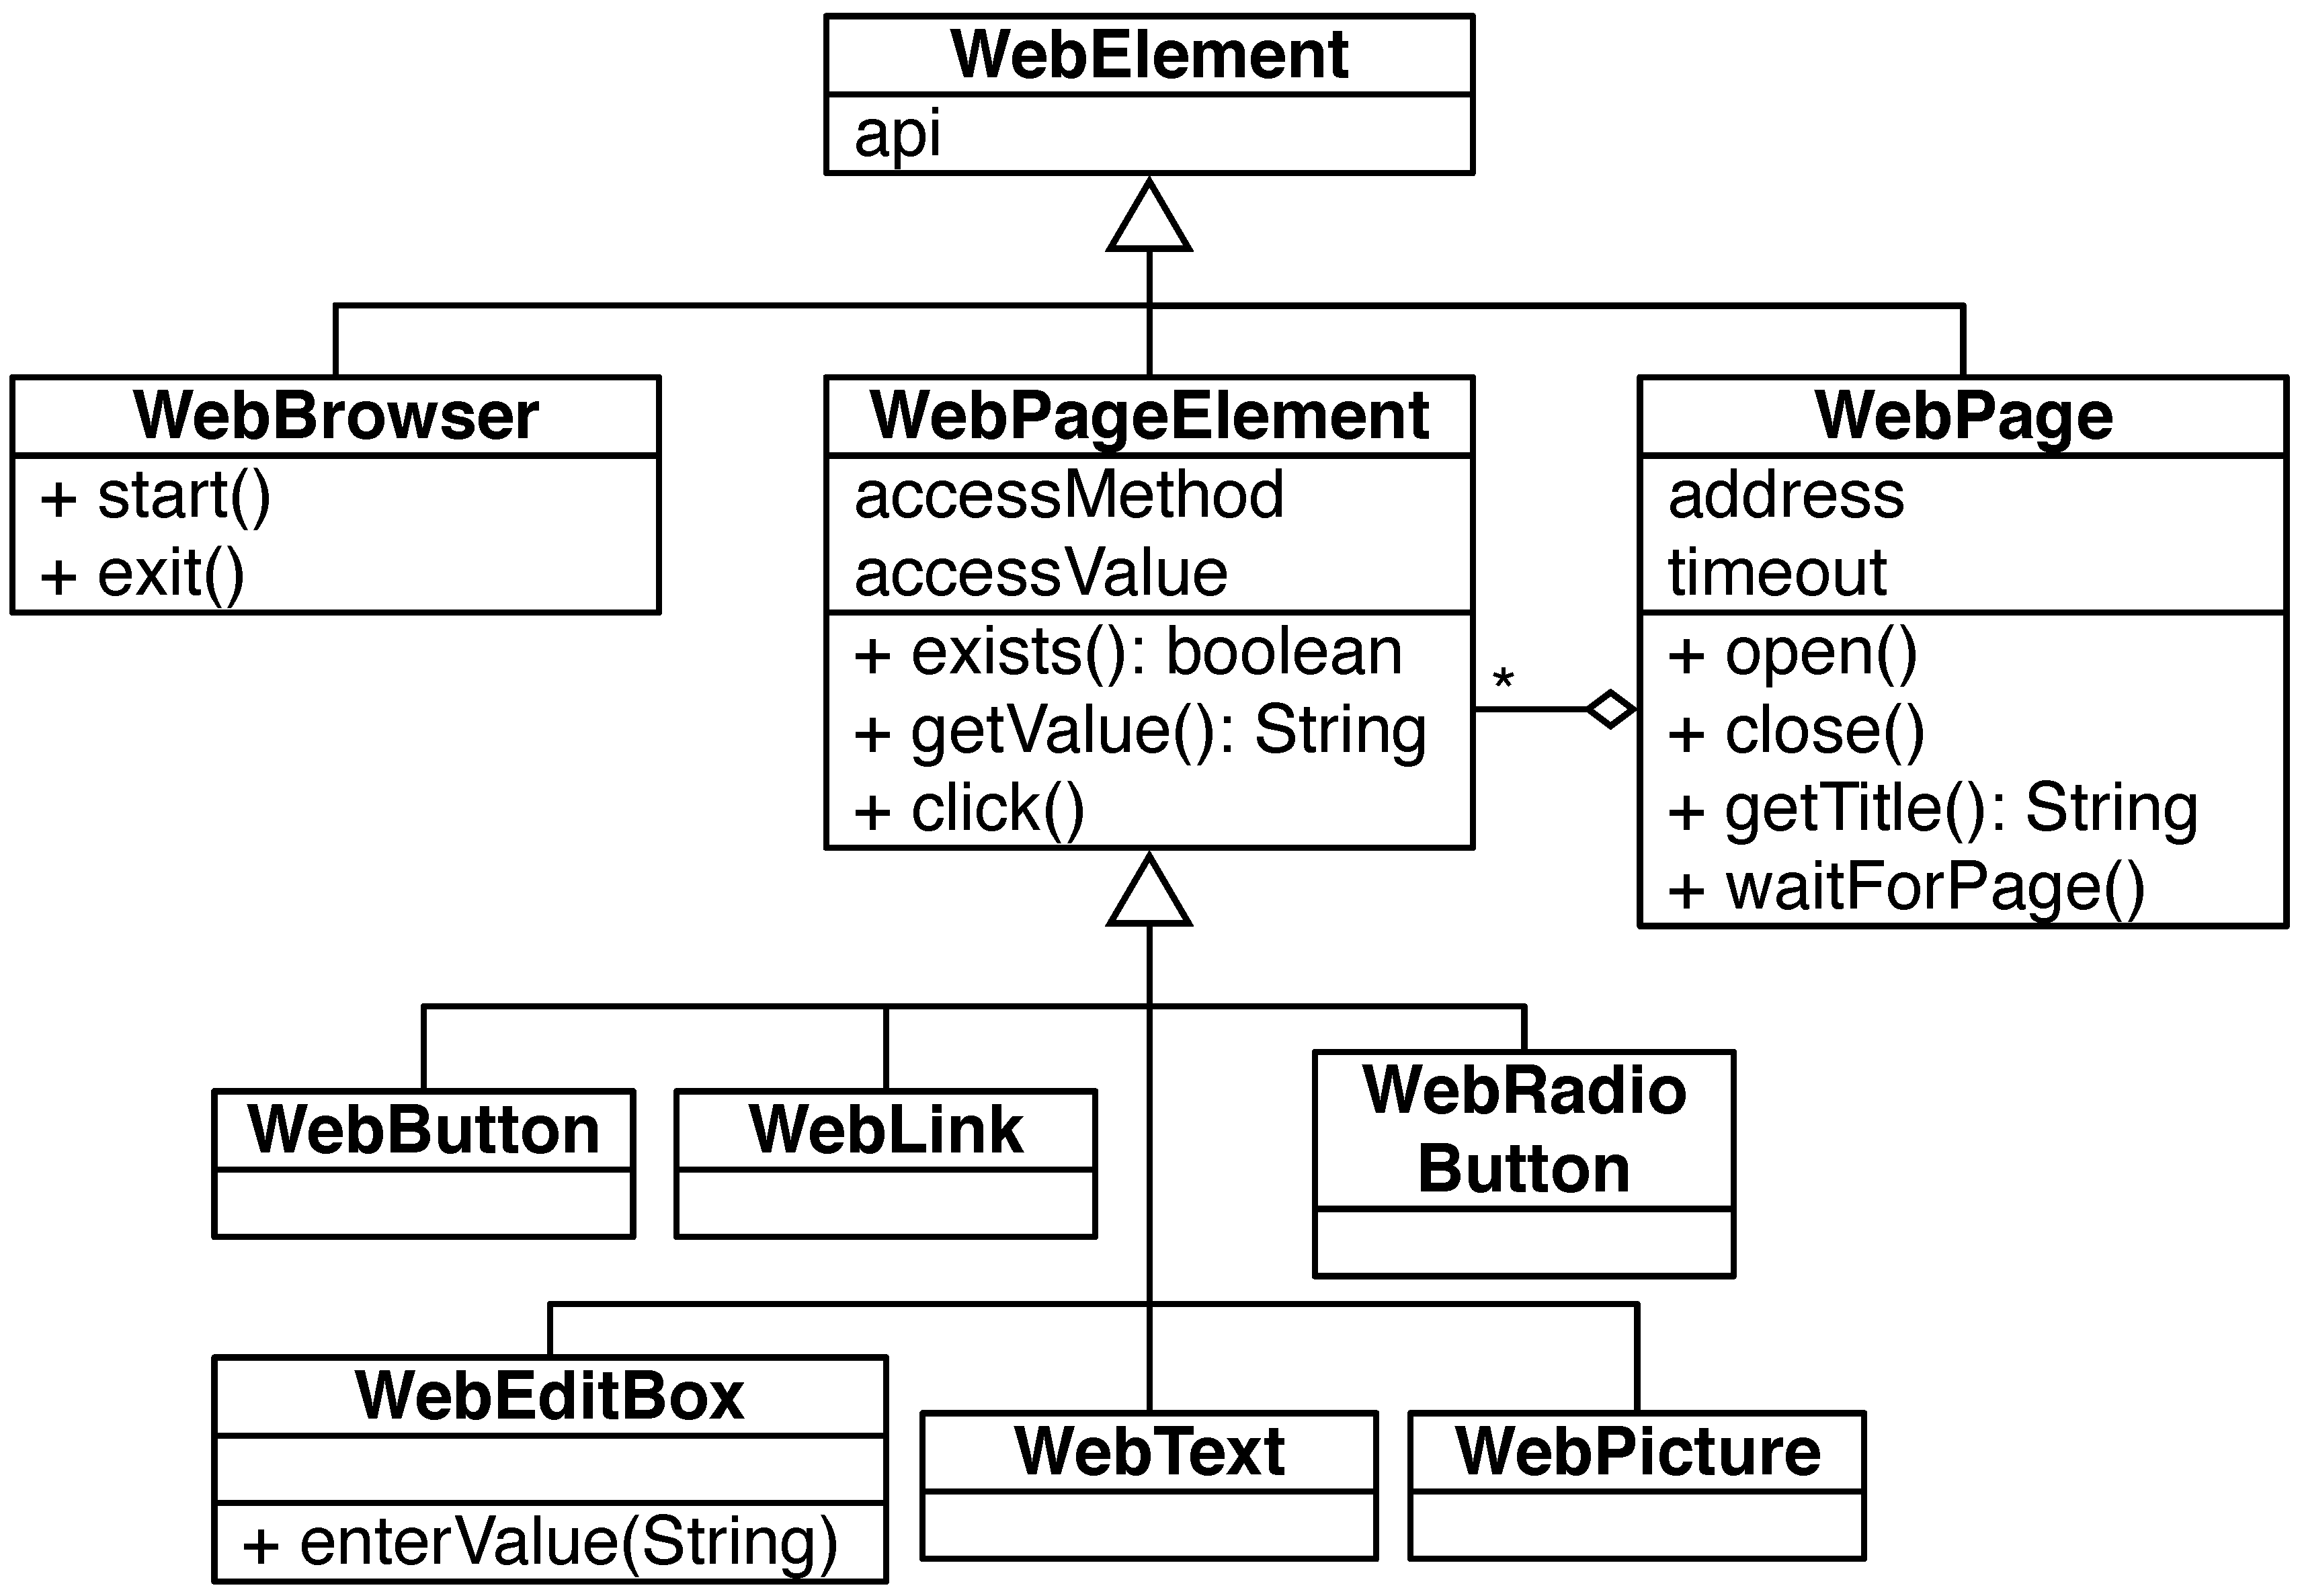
\includegraphics[width=90mm]{abscon-WebappUImodel}
	\caption{Web-applications SUT's interface class diagram (\texttt{web})}
	\label{fig:abscon:WebappUImodel}
\end{figure}

A SUT's interface model describes for a particular family of SUTs the different elements accessible when performing black-box testing. For instance, for Web-applications, the \texttt{web} model at line \ref{lst:abscon:xmltestcase:uimodel} in Listing \ref{lst:abscon:xmltestcase} is defined (here using a class diagram notation to ease the reading) in Figure \ref{fig:abscon:WebappUImodel}. It described the different elements we can found on a Web page: each class has to access the QTaste Selenium test API (using inherited attribute \texttt{api}) and will extend \texttt{WebElement};  \texttt{WebBrowser} objects will \texttt{start} and \texttt{exit} the Web browser specified for the current test case execution using the data from the external CSV file (as on line 6 in Listing \ref{lst:abscon:testcase}); a \texttt{WebPage} is available at a given URL  \texttt{address}, may be opened (and expected to load before a given \texttt{timeout}), closed, and has a title; \texttt{WebElement}s will appear on this page, each one is accessible using an \texttt{accessMethod} (\eg XPath) and an access value (\eg an XPath query to this element), may or may not exist on the page, has a value, and may be clicked;  the different elements we identified (relevant for the examples of this paper) are \texttt{WebButton}, \texttt{WebLink}, \texttt{WebRadioButton}, \texttt{WebText}, \texttt{WebPicture}, and \texttt{WebEditBox} which may be filled using textual values. 

\begin{lstlisting}[language=Python,
float,
label=lst:abscon:uimapping,
caption={Google instant search interface model instance (\texttt{UiMapping.py})}]
from uimodel_web import *

#mapping definitions
googlePage = WebPage("https://www.google.be/", 5000)
searchBar = WebEditBox("id", "lst-ib") (*@\label{lst:abscon:uimapping:searchbar}@*)
searchButton = WebButton("name", "btnK")
disableInstSearch = WebRadioButton("xpath", "//div[@id='instant-radio']/div[3]/span") (*@\label{lst:abscon:uimapping:disable}@*)
enableInstSearch = WebRadioButton("xpath", "//div[@id='instant-radio']/div[2]/span") (*@\label{lst:abscon:uimapping:enable}@*)
...
\end{lstlisting}

In AbsCon, each interface model is defined in Python. For one particular SUT's interface, this model is instantiated to represent the elements accessible to the test cases. For instance, for Google instant search, the \texttt{web} model instance is defined in \texttt{UiMapping.py} (Listing \ref{lst:abscon:uimapping}), as specified at line \ref{lst:abscon:xmltestcase:uimapping} in Listing \ref{lst:abscon:xmltestcase}. Each object is built using the dedicated constructor, which will require in most cases an access method and an access value: \eg search bar is accessed using its \texttt{id} in the page, which is \texttt{lst-ib} (line \ref{lst:abscon:uimapping:searchbar}), or using an XPath expression (lines \ref{lst:abscon:uimapping:disable} and \ref{lst:abscon:uimapping:enable}).
%
As for test APIs, interface models may be reused across different SUTs, as long as they share the same kind of interface (Web pages in this case).

%--------------------------------------------
\subsection{Assertions and actions mapping}
%--------------------------------------------

AbsCon extracts assertions and actions from the abstract test cases (Listing \ref{lst:abscon:xmltestcase}). Each assertion is mapped to a verification (\ie a function returning true or false) over the SUT's interface; and each action is mapped to a sequence of operations over elements of the SUT's interface (\ie again, a function). 

Verifications as well as operations are defined using the interface model instance defined in \texttt{UiMapping.py} (and will manipulate the different elements using the methods defined for those elements) and the QTaste data mapping mechanism in order to retrieve data from the external \texttt{TestData.csv} file. The mapping between the assertions and actions from the abstract test case is done by using the same name for the verifications and operations functions.

\begin{lstlisting}[language=Python,
float,
label=lst:abscon:operations,
caption={Verifications and operations mapping (\texttt{Operations.py})}]
from qtaste import *
from UiMappings import *

#Actions definition
def goHomePage():
	googlePage.open() 

def inputSearchString(): (*@\label{lst:abscon:uimapping:inputSearchString}@*)
	searchBar.enterValue(testData.getValue("SEARCHVALUE"))
...
#Asserts definition
def searchResultsPrinted(): (*@\label{lst:abscon:uimapping:searchResultsPrinted}@*)
	googlePage.waitForPage()
	if (not(navPicture.exists())):
		time.sleep(3) # wait for loading and retry
	return navPicture.exists()
...
\end{lstlisting}

For instance, Listing \ref{lst:abscon:operations} presents the verifications and operations mapping (\texttt{Operations.py}) for the Google instant search test cases from Listing \ref{lst:abscon:xmltestcase}. Function \texttt{inputSearchString} (line \ref{lst:abscon:uimapping:inputSearchString}) corresponds to the action with the same name in the test cases and inputs a search string, coming from the \texttt{SEARCHVALUE} column of the external CSV file, in the Google search bar defined in \texttt{UiMappings}. Function \texttt{searchResultsPrinted} (line \ref{lst:abscon:uimapping:searchResultsPrinted}) corresponds to the assertion with the same name in the test case, and returns true if the navigation picture from the result page is loaded.

%------------------------------------------------
\subsection{Test cases generation and execution}
%------------------------------------------------

Once the mappings are defined, AbsCon generates concrete (\ie executable) test cases for QTaste: for each test case, it  creates a Python script which imports the mappings and executes a sequence of \texttt{doStep} and \texttt{doAssert} calls using the verifications and operations functions. Those Python files, with the \texttt{TestData.csv} file, are used as input for QTaste to execute the test cases on the SUT and generate a summary test report.

Listing \ref{lst:abscon:testcasedef} presents the result of the generation for test case \ref{testcase1}: each \texttt{doStep} call (part of the standard QTaste API) corresponds to one action in the test case and will execute the given function. The \texttt{doAssert} function, defined by AbsCon, calls the given function (corresponding to an assertion in the test case) and prints the given error message if the call returns false. 
 
\begin{lstlisting}[language=Python,
float,
label=lst:abscon:testcasedef,
caption={Generation result for test case \ref{testcase1}}]
from qtaste import *
from Operations import *

#Assert
def doAssert(method, message):
	res = method()
	if res == 0:
		raise QTasteTestFailException(message)

#Steps
doStep(start)
doStep(goHomePage)
doAssert(onHomePage, "assertion onHomePage has failed")
doStep(inputSearchString)
doAssert(searchResultsPrinted, "assertion searchResultsPrinted has failed")
...
\end{lstlisting}


%%%%%%%%%%%%%%%%%%%%%%%%%%%%%%
\section{Implementation}
%%%%%%%%%%%%%%%%%%%%%%%%%%%%%%

\label{sec:abscon:architecture}

QTaste's plugin development functionality has been developed for specific requests made to QSpin. To the best of our knowledge, there is no plugin developer documentation available, but thanks to a QSpin developer guidance in the GitHub repository (where some examples of basic QTaste plugins are available), the development of AbsCon plugin was made possible. Basically, the plugin mechanism allows one to build his own user interface in a specific area inside the QTaste's user interface. Plugins have to be developed in Java (like QTaste) and must use the standard QTaste libraries. 

%-------------------------------------
\subsection{Graphical user interface}
%-------------------------------------

\begin{figure*}[t]
	\centering
	\subbottom[Main tab]{\label{fig:printscreen:main}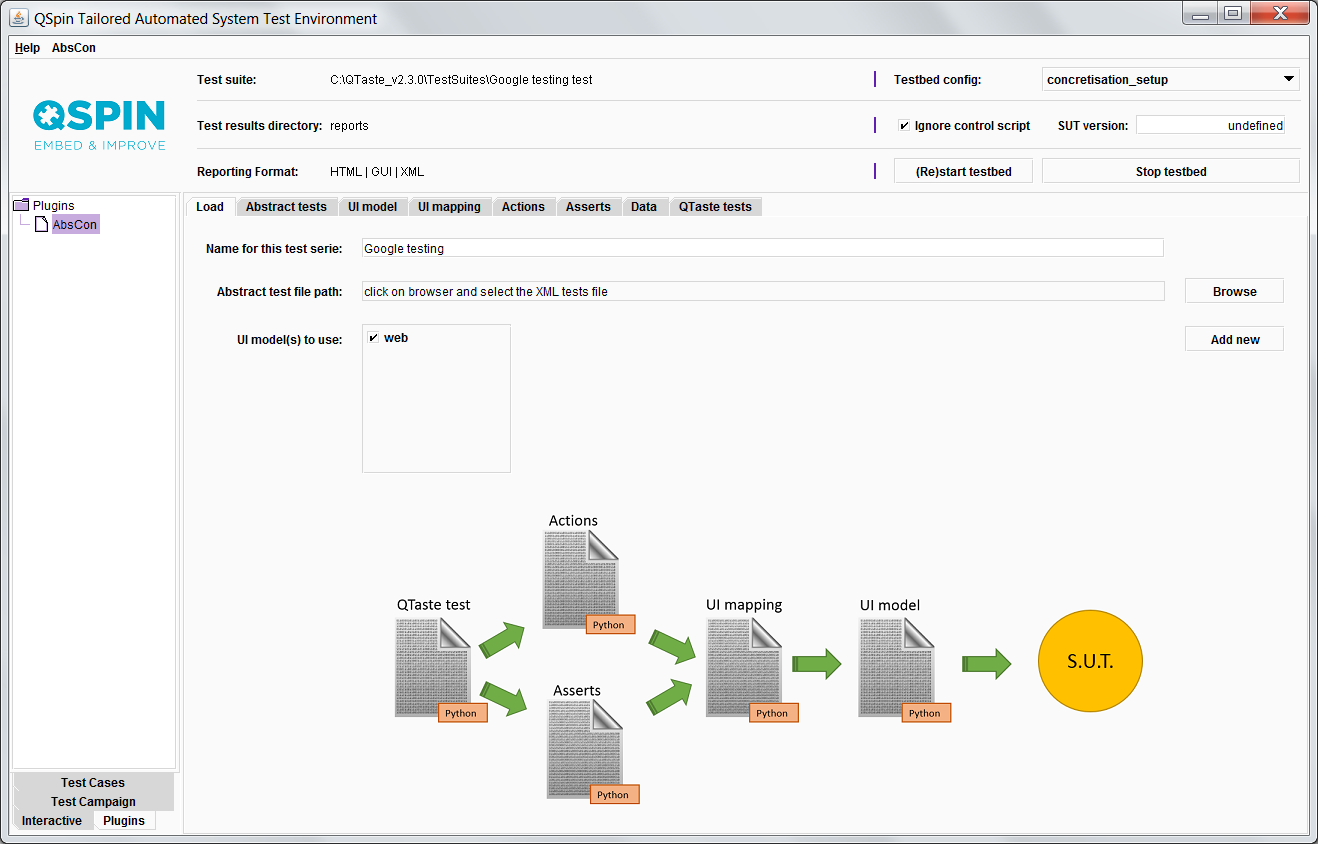
\includegraphics[width=0.99\textwidth]{abscon-main}}\\
	\subbottom[SUT interface mapping tab]{\label{fig:printscreen:uimapping}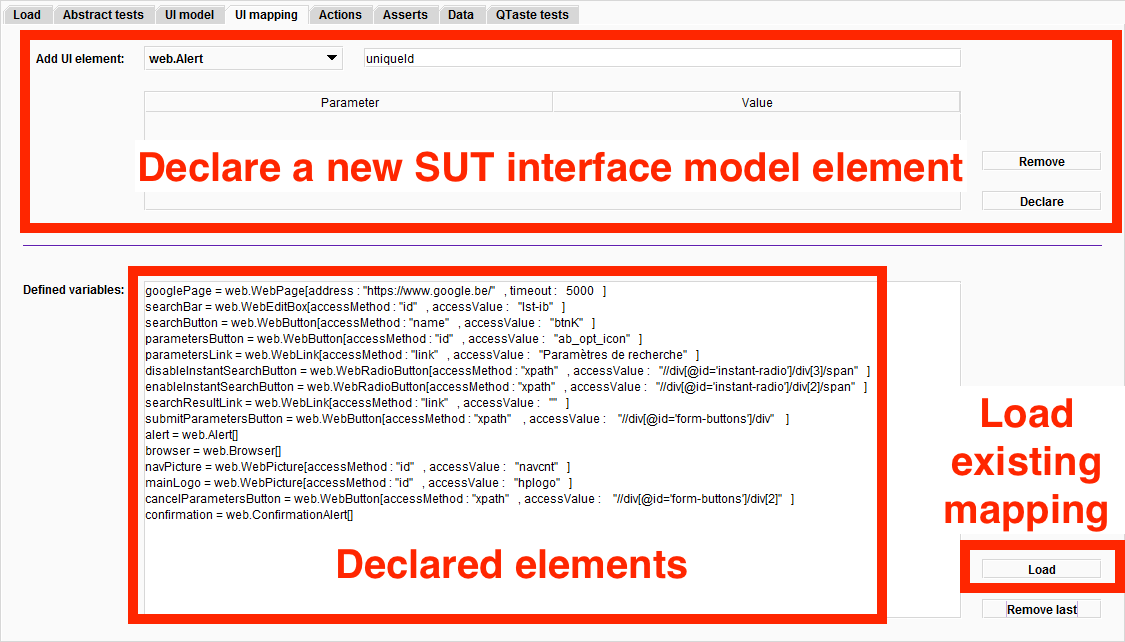
\includegraphics[width=0.44\textwidth]{abscon-uimapping}}
	\hspace{5pt}
	\subbottom[Assertions mapping tab]{\label{fig:printscreen:verifmapping}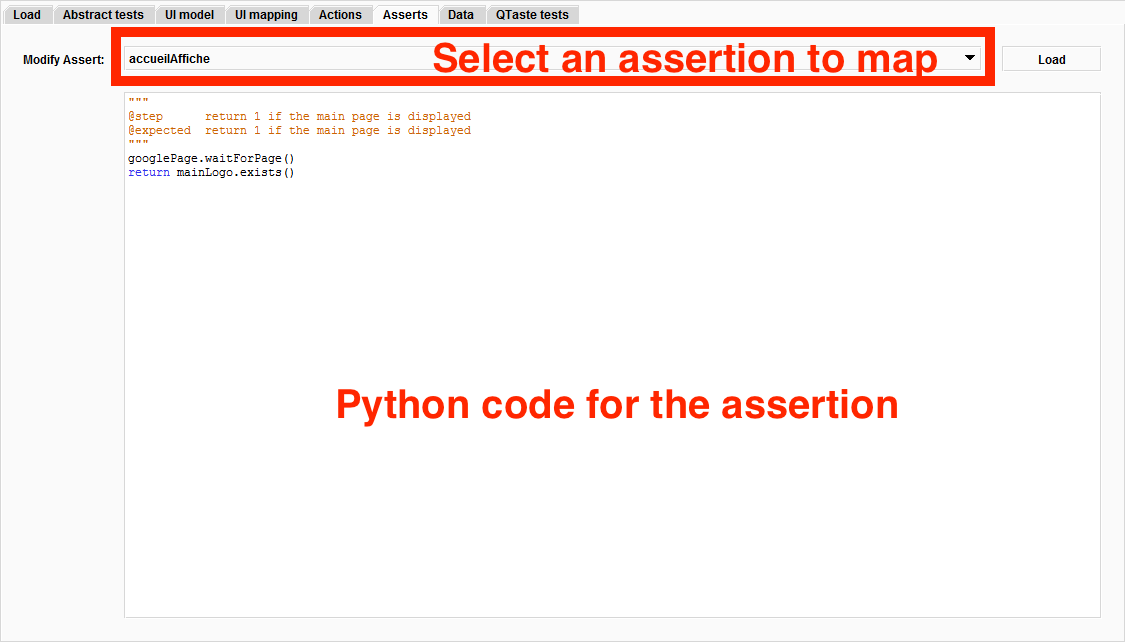
\includegraphics[width=0.44\textwidth]{abscon-asserts}}
	\caption{AbsCon plugin printscreens}
	\label{fig:printscreen}
\end{figure*}

AbsCon provides a graphical user interface integrated into QTaste (as shown in Figure \ref{fig:printscreen:main}) with different tabs, one for each mapping phase. When executing the plugin, the first step is to load the abstract test cases from an external XML file, AbsCon extracts the different actions and assertions for which a mapping has to be provided and presents them under the \texttt{Abstract tests} tab. 
The second step is to define or load a SUT's interface model (under tab \texttt{UI model}) and to instantiate this model under the \texttt{UI mapping} tab presented in Figure \ref{fig:printscreen:uimapping}: for each element of the interface, one has to instantiate a class of the interface model (selected using a drop-down list) by providing the required parameters for the constructor, and add it to the mapping using the \texttt{Declare} button (or load an existing mapping using the \texttt{Load} button). Actions and assertions mappings are given using the two next tabs: the user select the action/assertion using a drop-down list and provides the Python code for this action/assertion as shown in Figure \ref{fig:printscreen:verifmapping} (the assertion mapping tab in this case). In the \texttt{Data} tab, the user provides the data in an editable table, and finally generates the QTaste executable test cases in the \texttt{QTaste tests} tab.

%---------------------------------------
\subsection{AbsCon plugin architecture}
%---------------------------------------

\begin{figure}[t]
	\centering
	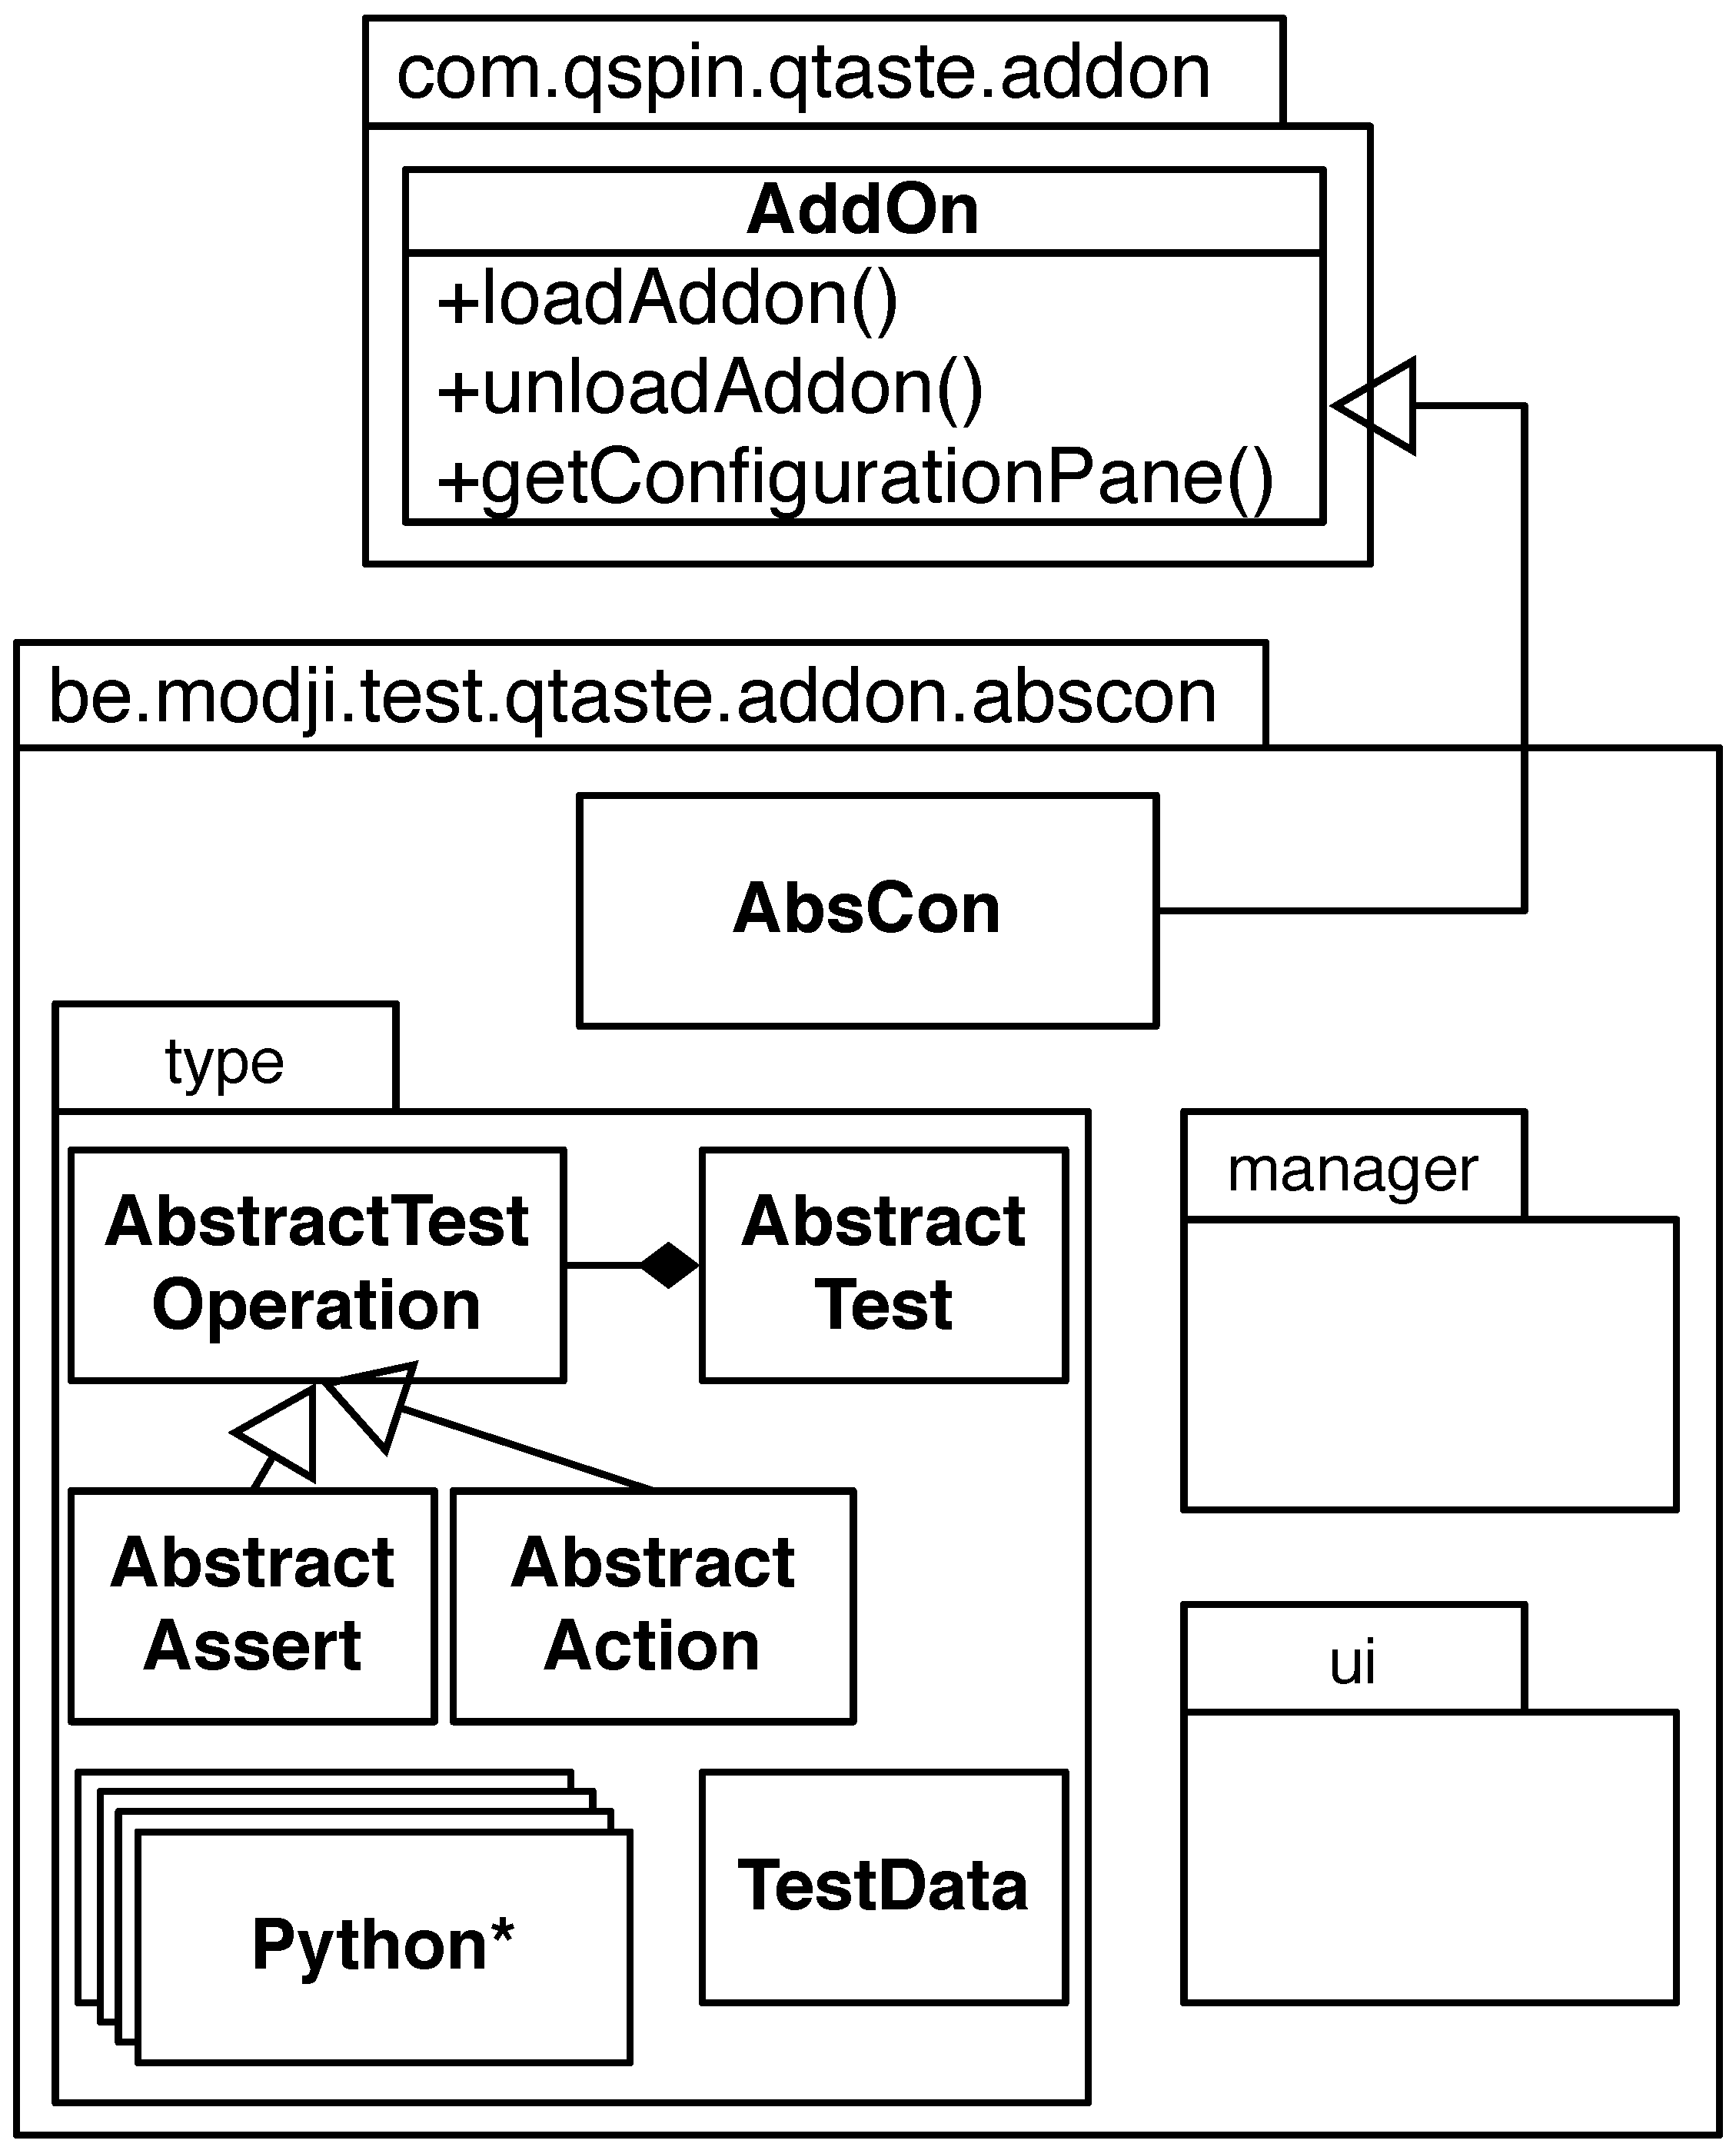
\includegraphics[width=60mm]{archi-packages}
	\caption{AbsCon packages diagram}
	\label{fig:abscon:archi-packages}
\end{figure}

Figure \ref{fig:abscon:archi-packages} gives an overview of the AbsCon packages diagram. The plugin architecture follows a classic model-view-controller pattern, divided in three Java packages: \texttt{type} one in charge of the model, \texttt{ui} package with all the classes in charge of the view, and \texttt{manager} one which contains the controller classes. 

The plugin execution is orchestrated by the \texttt{AbsCon} class, which extends the \texttt{AddOn} QTaste class: it overrides the \texttt{loadAddon}, \texttt{unloadAddon} and \texttt{get\-Confi\-gu\-ra\-tion\-Pane} methods. The two first contain all the operations to perform when QTaste loads or unload the plugin and its functionalities. The third one is the method that gives to QTaste environment the user interface of the AddOn (\ie it returns a \texttt{JPanel} that contains the plugin graphical user interface).

Model classes (package \texttt{type}) implement the different concepts presented in section \ref{sec:abscon:abscon}: abstract test cases (\texttt{AbsractTest}) are represented as a sequence of assertions (\texttt{AbstractAssert}) and actions (\texttt{AbstractAction}). The SUT's interface model and the assertions and actions mapping are encoded using Python (classes \texttt{PythonClass}, \texttt{PythonConstructor}, \texttt{PythonMethod}, and \texttt{PythonParameter}, abbreviated \texttt{Python*} in Figure \ref{fig:abscon:archi-packages}). 

Finally, the data feeding the CSV file used by QTaste during test cases execution is represented by the  \texttt{TestData} class. Manager classes (from the \texttt{manager} package) play a role of controller during the plugin execution and dialogue with the classes from the \texttt{ui} package, in charge of the AbsCon plugin graphical user interface.


%---------------------------------------
\subsection{Source code}
%---------------------------------------

AbsCon is released as an open source project on GitHub, under the GNU public license. It can be downloaded at the following address: \url{https://github.com/modji-be/AbsCon}. The project is written in Java and has 34 classes, 248 methods, and 4864 lines of code.

%%%%%%%%%%%%%%%%%%%%%%%%%%%%%
\section{Discussion}
%%%%%%%%%%%%%%%%%%%%%%%%%%%%%

\label{sec:abscon:discussion}

In this section, we discuss AbsCon's abstraction and user interface modelling mechanisms, maintenance costs, and mappings, based on our experience with the tool. A complete and rigorous evaluation of the tool, using a controlled experiment \cite{Wohlin2000} with test engineers, is left for future work.

\paragraph{Abstraction:}
%-------------------------

AbsCon heavily relies on \emph{abstraction}, of the SUT's interface on the one hand, and on the assertion and actions on the other hand. This abstraction layer allows to define each mapping independently from the higher or lower levels: abstract test cases are defined using assertions and actions with meaningful names for the user/test engineer; each assertion and each action is mapped to a Python function representing a verification or an operation, and is defined as a manipulation of the SUT's interface meaningful from a user point of view (depending on the nature of the SUT, the user may be a human or another system), thanks to the SUT's interface model; finally, the SUT's interface model encapsulates the test API calls in charge of the effective communication with the SUT. 

\paragraph{User interface modelling:}
%-------------------------------------

Another option to the modelling of the SUT's interface described in this chapter would be to use \glspl{UIDL} \cite{Guerrero-Garcia2009} such as USIXML \cite{Limbourg2005}. These languages provide generic constructs (organized in one or more metamodels that represent both platform independent and platform specific views, according to Model-Driven Architecture principles \cite{Kleppe2003})  allowing to model any kind of user-interface (including non-conventional interfaces such as voice-enabled ones). 

However, the use of such proposals in ours raises the following problem: the number of concepts they are offering being quite large, modelling a simple user interface can be cumbersome and complex, unless we tailor the language to specific needs. In our context, we do not to try to model the whole user interface but the subset concerned by the tests. We therefore adopted a lightweight approach that has the complementary advantage of not requiring any new modelling language to learn, by exploiting Python's object-orientation facilities.  Furthermore, as initially mentioned, QTaste's spectrum is larger than testing graphical user interfaces.


\paragraph{Maintenance costs:}
%-----------------------------

The goal of our abstraction layer is to reduce the overall complexity of the test cases and to decrease the \emph{maintenance costs}. Indeed, when the SUT's interface evolves, only the mapping to this interface has to be (potentially) changed, AbsCon can then re-generate concrete test cases for QTaste that will serve for non-regression. This process is much lighter than the update of QTaste test cases as it will (potentially) require to update all the test cases containing code that manipulate the SUT's interface (using directly the test API in this case). In the same way, when functionalities are added to the SUT, only the new interface elements, and verifications and operations mappings have to be added. New abstract test cases may then be written for those elements and AbsCon can re-generate a complete set of test cases for the whole SUT.

\paragraph{Mappings:}
%-------------------

The definition of the different mappings may represent an additional effort during test activities. However, different aspects have to be taken into account. First, the SUT's interface model depends solely on the nature of the SUT, \eg Web-application for the \texttt{web} model from Figure \ref{fig:abscon:WebappUImodel}. Once defined, this model may be reused across different projects. As this model abstracts the test API by defining methods from the interface point of view (\eg \texttt{click}, \texttt{open}, \texttt{getTitle}, \etc in Figure \ref{fig:abscon:WebappUImodel}), we believe that it will also soften QTaste's learning curve. Second, the definition of the mappings enables integrating existing model-based testing techniques (\eg \cite{Utting2007,vibes}) rather than defining a new complete test development process.   

In our opinion, the most time consuming task will be to \emph{identify} and \emph{map} the different SUT's \emph{interface elements}. This cost may be reduced in some cases using existing tools: for instance, \textit{Inspect} \cite{inspect}  or \textit{SwingInspector} \cite{swinginspector} are tools used to identify and access graphical user interface elements in classical desktop applications. In our \texttt{UiMapping.py} example in Listing \ref{lst:abscon:uimapping}, we used Firefox's inspection tool to identify the different elements on a Web page. Depending on the nature of the SUT, this mapping may also be partially or totally automated (this will be part of our future works), like for Web-applications for which each element on a Web page describes itself using HTML tags. 


%%%%%%%%%%%%%%%%%%%%%%%%%%%%%%%%%%%%
\section{Related work}
%%%%%%%%%%%%%%%%%%%%%%%%%%%%%%%%%%%%

\label{sec:abscon:relatedwork}

Test case \gls{concretization} techniques are classified by Utting \textit{et al.} \cite{Utting2007} in 3 categories: \emph{adaptation} approaches abstracts the SUT by using a wrapper (also called an adapter), test cases call this wrapper in order to execute operations on the SUT; \emph{transformation} approaches transform abstract test cases into test cases directly executable by the SUT, possibly using  additional information; and \emph{mixed} approaches also transform abstract test cases in executable test cases, but using an adaptation layer in order to abstract the SUT. Using this classification, QTaste uses adaptation to abstract the SUT using its test APIs and requires to write test cases which will use those test APIs. 

There exists other adapters, like \emph{Selenium} and \emph{Sahi} \cite{sahi} to test Web-applications, or \emph{AutoHotKey} \cite{ahk} to test Windows applications. Tools like \emph{Sikuli} \cite{sikuli} and \emph{Squish} \cite{squish} provide adaptation mechanisms to perform graphical user interface testing using techniques like image recognition, or recording and playback. None of these tools natively support abstract test case \gls{concretization}.

Other transformation and mixed tools like \emph{TOTEM}~\cite{Briand2001}, \emph{SpecExplorer}~\cite{Veanes2008}, \emph{MaTeLo}~\cite{Dulz2003}, \emph{Smartesting} solutions~\cite{smartesting}, or \emph{STALE}~\cite{Li2015} implement full model-based testing approaches, including abstract test case generation and concretization from different modelling languages (\eg UML Testing Profile \cite{Williams2007}, etc). 

Rather than having a complete transformation chain (from models to executable test cases), we developed AbsCon in order to plug it on an existing approach (VIBeS in this case), concretize abstract test cases, no mater their origin as long as they are described as sequences of actions and assertions, and get executable test cases on a generic and industrial test environment like QTaste.

As for VIBeS, other model-based testing approaches produce abstract test cases that are concretized using existing tools, this is the case for \emph{Skyfire}~\cite{Li2016a} which uses a transformation approach to produce \emph{Cucumber}~\cite{cucumber} abstract test cases from UML diagrams. Cucumber is a popular behaviour-driven development tool that aims at producing typical examples of the behaviour of a system under development, described using a semi-structured language: \emph{Gherkin}. Those examples are used as acceptance tests and concretized using a Java annotations based mechanism, mapping semi-structured sentences to Java methods using a defined string pattern. The executable test cases are run in standard JUnit environment. 
%
Cucumber could have been another test execution environment target, but, to the best of our knowledge, it does not provide any SUT's interface abstraction mechanism (like QTaste's test APIs) and would have required more effort to define a programmer friendly abstraction mechanism of this interface.


%%%%%%%%%%%%%%%%%%%%%%%%%%%%%%%%%%%%
\section{Wrap up and perspectives}
%%%%%%%%%%%%%%%%%%%%%%%%%%%%%%%%%%%%

\label{sec:abscon:conclusion}

In this chapter, we presented \gls{AbsCon}, a QTaste plugin developed to concretize abstract test cases represented as sequences of actions and assertions. The adaptation mechanism provided by QTaste's test API is enhanced by a programmer friendly way to encapsulate the calls to this API using a common model specific to the kind of the SUT's interface. This model, \emph{reusable} for different SUTs as long as their interface are of the same kind, defines the possible interactions with the SUTs. An instance of this model, specific to a SUT, is used in operations and verifications corresponding to actions and assertions defined in the abstract test cases. Using the different mappings, AbsCon is able to generate test cases executable in QTaste.

Originally developed to bridge the gap between VIBeS and concrete test cases, AbsCon offers multiple advantages, even in a non model-based testing context. We chose to implement it over an existing industrial test case management and execution tool, which will, we believe, eases its broader adoption. As a standalone tool (\ie not used in an model-based testing chain), AbsCon enhances QTaste's \emph{genericity} by \emph{raising the abstraction level} of different elements: the SUT's interface and test APIs, thanks to the SUT's interface model mechanism; and the test cases themselves by allowing to provide definitions using abstract actions and assertions (which is  to the user) instead of Python scripts. 

So far, the plugin has only been used on small examples, a more complete validation is part of our future works. We will also explore automated SUT's interface mapping possibilities using existing inspection tools. Finally, another potentially interesting research direction is the definition of the test cases using a structured natural language (like Gherkin \cite{cucumber}) as an input to AbsCon instead of XML files. 
This could be used to automatically define, not only the actions and assertions, but also the data to use during the test cases execution. Ideally, the definition of the test cases in a structured language would be processed by AbsCon to populate both the list of assertions and actions to map, the elements of the SUT's interface to use (based on the text describing the test cases steps), and the CSV file used by QTaste. 

More details on \gls{AbsCon} can be found in Jeremy Vanhecke's master thesis \cite{Vanhecke2016}.



%%%%%%%%%%%%%%%%%%%%%%%%%%%%%%%%%%%%%%%%%%%%%%%%%%%%%%%%%
\part{Postface}
%%%%%%%%%%%%%%%%%%%%%%%%%%%%%%%%%%%%%%%%%%%%%%%%%%%%%%%%%
\label{part:postface}

\chapter{Conclusion and future research directions}
\label{chap:conclusion}

Software product line testing is a complex, yet essential, task to guarantee a \emph{good enough} quality level of the products. The test engineer has to compromise between the large number of products to test and a limited testing budget. This requires a strong and usable framework to support the whole testing process, from test case selection at the domain level to test case concretization into a test script for one particular product.

In this thesis, we present a model-based \emph{behavioural} \gls{SPL} testing framework. Our approach relies on formal ground without sacrificing usability in a unified and flexible enough model-driven framework. We believe that this combination will foster the usage of efficient SPL testing techniques, thus improving the confidence in the SPL paradigm.

%%%%%%%%%%%%%%%%%%%%%%%%%%%%%%%%%%%%%%%%%
\section{Summary of contributions}
%%%%%%%%%%%%%%%%%%%%%%%%%%%%%%%%%%%%%%%%%

By working on domain artefacts with a \gls{FTS} and a \gls{feature model}, we developed a\emph{ behavioural family model-based testing framework}. The output of the whole chain is a \gls{test suite} for, potentially, one product, a subset of products or even the whole product line according to the provided selection criteria. We consider three types of criteria: criteria based on the \emph{structure} of the FTS; criteria based on a \emph{dissimilarity heuristic}; and criteria based on \emph{usages} of the SPL. 
%
%In this thesis, structural, dissimilar, and usage criteria are considered separately. Future work includes \emph{combination} of those criteria in order to refine the test case selection using for instance evolutionary algorithms. We believe that this will help to design test suites compromising between several objectives: \eg the number of test cases, the number of products to test, the usage of the SPL (to perform regression testing for instance), \etc 
%Those objectives may also be extended to non-functional properties coming from the feature model (\eg features cost or features popularity) or the behavioural model (\eg time, probabilities of failure, \etc). 

As a complement to selection criteria, mutation testing allows to improve a test suite by assessing its quality using mutation analysis and select test cases for the live mutants. To face the cost of such analysis for a large number of mutants, we propose to take advantage of the variability formalisms to compactly represent all possible mutations in a single model: the \emph{\acrfull{FMM}}. In a \gls{FMM}, each feature represents a mutation: \ie a model transformation representing the application of a mutation operator on the model. It allows to generate mutants of any order and assess test effectiveness via an optimised execution scheme.

To detect equivalent mutants that may impair the analysis, we offer two baseline algorithms based on \emph{random simulation}, and compare them to \emph{language equivalence} under weak and strong mutation scenarios. Our evaluations suggest to use simulations first to quickly discard many non-equivalent mutants, and then employ exact approaches only on a small amount of probably equivalent mutants to speed up equivalence analysis.

Our framework, called \emph{\gls{VIBeS}}, is implemented in Java as an open-source modular Maven project. Each module is dedicated to one particular aspect of the testing activities. Each one has a dedicated API and is also encapsulated in a Java DSL to simplify usages.
VIBeS is the reference implementation to assess the different elements presented in this thesis. Our empirical assessments are performed on several case studies, representing embedded systems, with manually defined models, and Web applications, with semi-automatically reverse engineered models. 


%%%%%%%%%%%%%%%%%%%%%%%%%%%%%%%%%%%%%%%%%
\section{Perspectives and future work}
%%%%%%%%%%%%%%%%%%%%%%%%%%%%%%%%%%%%%%%%%

This section presents our perspectives and future potential research directions to improve test case selection and model-based product line mutation analysis. 

%Future work includes refinement of this reverse engineering process by, for instance, inferring feature expressions of the transitions of the FTSs. We also intend to analyse the test suites generated using the different selection criteria using mutation testing to discover potential subsuming relationships between them.

%-----------------------------------------------------------------
\subsection{Test case selection}
%-----------------------------------------------------------------

Test case selection may be improved in different ways: we limit ourselves to two possible directions, presented hereafter.

\paragraph{Multi-objectives selection:}
%-------------------------------------------------

Although we consider structural, dissimilar, and usage criteria separately, we may \emph{combine} those different approaches in order to refine the test case selection. Typically, test case selection using structural criteria, when applied to an FTS, becomes a compromise between the coverage of the behavioural model, the number of test cases selected, and the number of products required to execute those test cases. \emph{Evolutionary algorithms}, like the one used for dissimilarity selection, can handle this kind of optimisation problems. 

Dissimilar test case selection can also be extended with different measures (\eg test cases structural coverage) as well as different ways to combine them to perform dissimilarity selection. For instance, the operator used to combine the different distances ($\otimes$) can be refined to take more measures into account and balance them, depending on their significance, to foster one or more particular distances.

Aspects other than usage or functional elements (like structural coverage or dissimilarity) of the product line may also play a role in the test case selection process. \Eg the cost (in time and/or material) linked to the configuration of some products can be taken into account: algorithms can be modified to prefer test cases requiring cheaper products for their execution. Recent developments in the SPL verification and validation community tend to consider more and more \emph{non-functional properties} of SPLs, both at the feature model level \cite{Siegmund2015,Siegmund2013,Parejo2016,Olaechea2014,Guo2013,Bartholdt2009,Etxeberria2008} and in the behavioural model (like usage information) \cite{Rodrigues2015,TerBeek2015b,Olaechea2016,terBeek2016}.
All this information can be used to tune the evolutionary algorithm to refine the test case selection.


\paragraph{Mutation coverage driven selection:}
%-------------------------------------------------

Since \textit{mutants are a valid substitute for real faults} \cite{Just2014},  we envision to develop test case selection techniques based on mutation coverage of a FMM. The idea is to select test cases designed to \emph{detect live mutants}, using for instance counter-examples generated by a FTS model checker tool \cite{Cordy2013}. This would allow to select, not only positive abstract test cases (test cases that the products should be able to execute), but also negative abstract test cases (test cases that the product should not be able to execute) \cite{Ammann1998}, enhancing the test case selections presented in Chapter \ref{chap:coverage}.

%-----------------------------------------------------------------
\subsection{Towards model-based product line mutation analysis}
%-----------------------------------------------------------------

\label{subsec:splmutationanalysis}

Model-based mutation analysis requires to use a set of mutation operators to produce mutants from the specification of the product line under test. Those operators are usually designed based on empirical studies build upon large error repositories, or on a fault model defined to list potential failure causes in a system \cite{Mathur2008}. McGregor \cite{McGregor2008} defines a fault model for software product lines and describes for each step of the product line development, the kind of fault that may appear. 

In the remainder of this section, based on the contributions of Chapter \ref{chap:mutation}, we sketch a vision of a complete \emph{model-based product line mutation analysis}. We discuss how our contributions and existing research literature on mutation testing contribute to this vision and point out future research directions. We consider the following artefacts as possible candidates for mutation:
\begin{itemize}
\item the feature model, defining how features may be combined to form valid products;
\item domain artefacts, reusable across several products (\ie the FTS);
\item the mapping between the feature model and the domain artefacts (\ie the feature expression labels); and 
\item the derivation process used to bind variability in the domain artefacts to get one product (\ie the FTS projection operator).
\end{itemize}
The last artefacts are the products themselves (that can be mutate using standard mutation techniques \cite{Jia2011a,Mathur2008}).

\paragraph{Feature model mutation:}
%------------------------------------

\Gls{feature model} mutation is already largely covered by literature to assess product sampling (in this case, test cases are valid products of the product line) and generate better samples \cite{Henard2014,Reuling2015a,Lackner2014,Arcaini2015a}, or to detect errors and repair feature models \cite{Henard2013b,Arcaini2016a,Arcaini2017}. This last line of research uses mutation on the feature model in order to automatically improve or repair it when an error or an inconsistency is found. We distinct two kinds of mutation operators: mutation operators working on the \emph{syntax} of the feature model and operators working on the \emph{semantic} of the feature model. Operators working on the semantic are operators working on the syntax of the formalism used to express the semantic of the feature model (\ie a boolean formula). We use syntax and semantic only to clearly distinct the abstraction level at which the mutation is performed.

\paragraph{Syntactic mutation:}
%-------------------------------

\begin{figure}
	\centering
	\subbottom[Original]{
		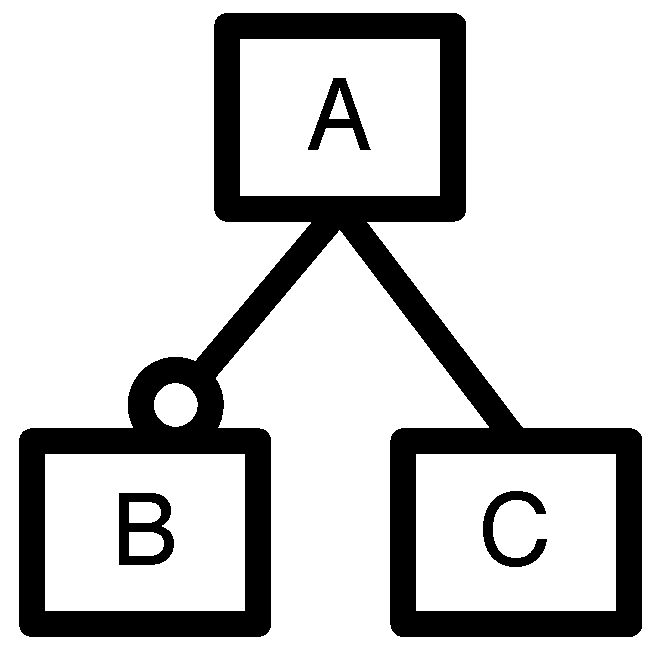
\includegraphics[width=15mm]{exemple-graphical-mutation-original}
		\label{fig:fmm:syntacticoriginal}
	}
	\subbottom[Mutant]{
		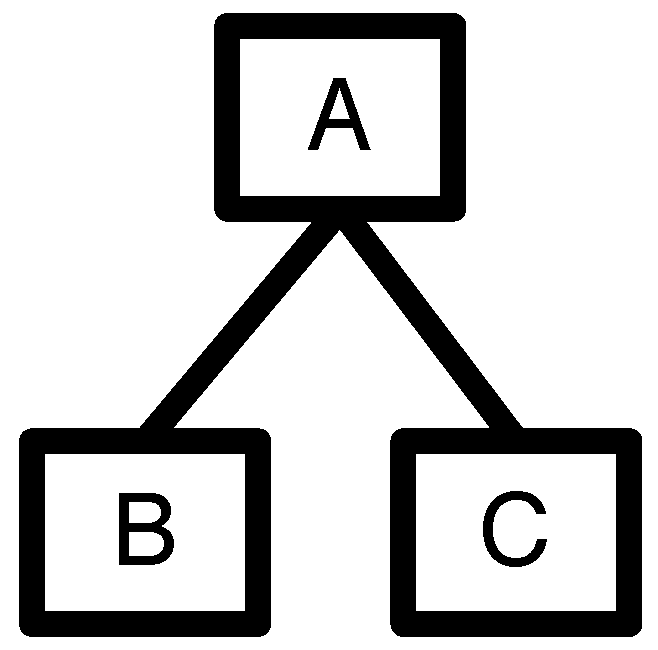
\includegraphics[width=15mm]{exemple-graphical-mutation-mutant}
		\label{fig:fmm:syntacticmutant}
	}
	\caption{Example of syntactic mutation of a feature model \cite{Arcaini2015a}}
	\label{fig:fmm:syntactic}
\end{figure}

Mutation operators working on the syntax of the feature model transform the graphical (or textual) representation of the feature model to produce a mutant. For instance, Arcaini \etal \cite{Arcaini2015a} define operators that will transform an alternative into a \textit{Or} or a \textit{And}, make an optional feature mandatory, change \textit{requires} constraint to \textit{exclude} constraint, \etc Figure \ref{fig:fmm:syntactic} presents an example of syntactic change in a small feature model: the optional constraint in Figure \ref{fig:fmm:syntacticoriginal} has been transformed to a mandatory feature in Figure \ref{fig:fmm:syntacticmutant}.

\paragraph{Semantic mutation:}
%-------------------------------

Semantic mutation works on the semantic of the feature model: a boolean expression over the features of the feature model \cite{Schobbens2007}. Application of those operators will first require a flattening of the feature model into a \gls{CNF} formula \cite{Henard2015b} and apply mutations on this formula. Henard \etal \cite{Henard2013b,Henard2014} use this strategy to select products to test in order to detect mutations of the feature model. The feature model is first transformed into a \gls{CNF} formula which is used an input for two mutation operators modifying on clause of the CNF formula. For instance, the feature model of Figure \ref{fig:fmm:syntacticoriginal} is transformed into the following CNF clause:
$$\fm = A \wedge (\neg B \vee A) \wedge (\neg C \vee A) \wedge (\neg A \vee C)$$
Which may then be mutated (using Henard \etal's \textit{second operator} \cite{Henard2013b}) to:
$$\fm_m = A \wedge \neg B \wedge A \wedge (\neg C \vee A) \wedge (\neg A \vee C)$$
%
Since the CNF formula represents the feature model, it is possible to show an equivalence between syntactic and semantic mutation operators. However, one application of a syntactic mutation operator may require several applications of semantic mutation operators (and \textit{vice versa}). For instance, the syntactic operator transforming an alternative to a \textit{And} will require several transformations on the CNF formula representing the feature model. 

\paragraph{Featured transition system mutation:}
%-------------------------------------------------

\begin{figure}
	\centering
	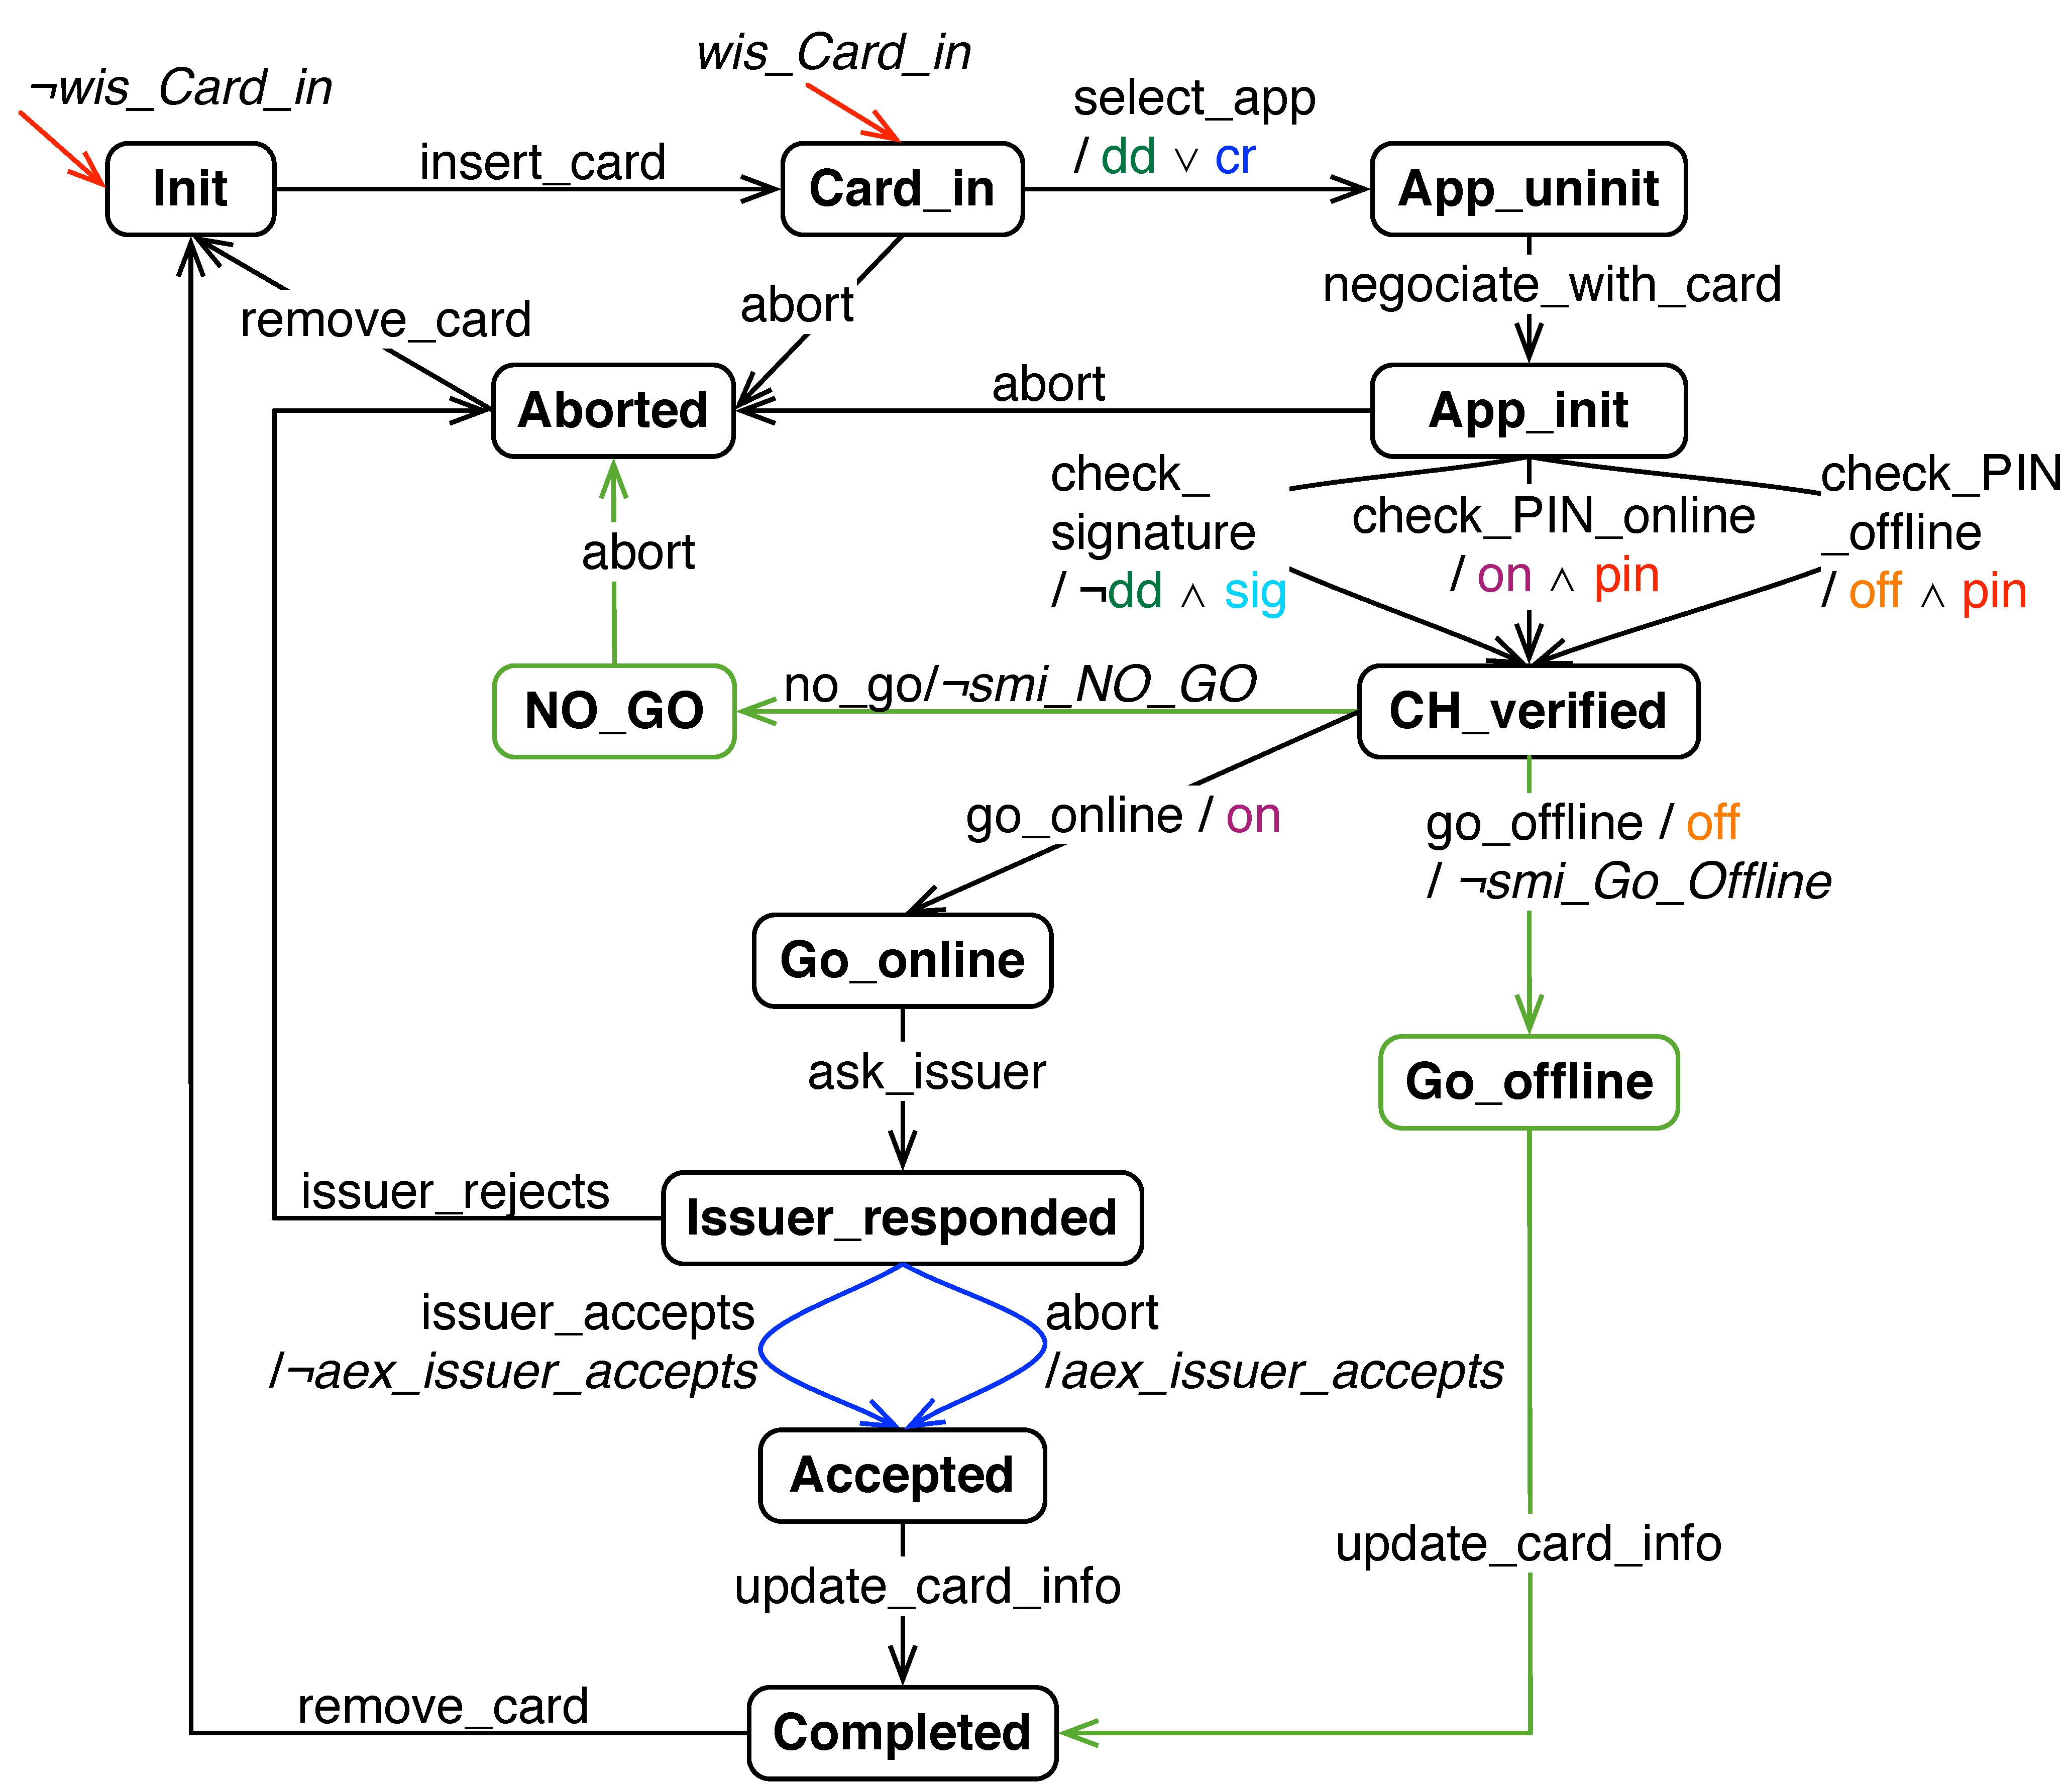
\includegraphics[width=95mm]{cpt-exemple-fts-fmm}
	\caption{Card payment terminal product line FFTS}
	\label{fig:fmm:ftsfmmexemple}
\end{figure}

\glspl{FTS} describe the behaviour of all the products of a product line. Mutate a FTS comes to modify the behaviour of a whole product line (or at least the products able to execute the modified part of the FTS). The mutation operators defined in Annex \ref{apdx:fmm:operators} may be used to produce mutants. In such case, the FMM has a FTS with two feature models and two $\gamma$ labelling functions. The first feature model $d_p$ and $\gamma_p$ function are used to represent all the products of the product line, and the second feature model $d_m$ and $\gamma_m$ function are used to represent all the mutants of the mutants family.
For instance, the result of the card payment terminal product line of Figures \ref{fig:cpterminalfts}, mutated using the state missing, action exchange, and wrong initial state operators, produces the FTS in Figure \ref{fig:fmm:ftsfmmexemple}. The FMM is composed of this FTS, the feature model of the product line (in Figure \ref{fig:cpterminalfm}), and the feature model of the mutants family (in Figure \ref{fig:fmm:cptmutantsfm}). 
As for feature model mutation, modifying the FTS using model transformations are \emph{syntactic mutations} and affects the product line as a whole. \Eg removing one transition using transition missing operator removes it for all the products of the product line.

\newcommand{\wFe}{\mathit{fe}}

One may want to mutate only the behaviour of a certain subset of products. In this case, the operators defined in Annex \ref{apdx:fmm:operators} have to be modified in order to consider only a given subset of products, represented as a feature expression $e$. For instance, if we mutate the following transition in an \emph{enumerative} way, with $e$ representing a subset of the products defined by the feature expression $\wFe$:
\begin{center}
\begin{tikzpicture}[>=stealth',shorten >=1pt,auto,node distance=4cm]
	\node[state] (s0) {$s_0$};
	\node[state] (s1) [right of=s0] {$s_1$};
	\path[->] (s0)  edge node {$\alpha_x / \wFe$} (s1);
\end{tikzpicture}
\end{center}
By applying the AEX operator to change action $\alpha_x$ to $\alpha_y$, but only for the subset of products designed by $e$, we have the mutant:
\begin{center}
\begin{tikzpicture}[>=stealth',shorten >=1pt,auto,node distance=4cm]
	\node[state] (s0) {$s_0$};
	\node[state] (s1) [right of=s0] {$s_1$};
	\path[->] (s0) edge node {$\alpha_y / \wFe \wedge e$} (s1)
	          (s0) edge [bend right=45] node [below] {$\alpha_x / \wFe \wedge \neg e$} (s1);
\end{tikzpicture}
\end{center}
Where the original transition is restricted to $ \wFe \wedge \neg e$ and the mutated transition is only activated for products respecting $\wFe \wedge e$ feature expression.
Using the \emph{\gls{FMM}} approach, we need to duplicate transitions to take the feature expression representing the mutant into account:
\begin{center}
\begin{tikzpicture}[>=stealth',shorten >=1pt,auto,node distance=4cm]
	\node[state] (s0) {$s_0$};
	\node[state] (s1) [right of=s0] {$s_1$};
	\path[->] (s0) edge node {$\alpha_x / \wFe / \neg aex$} (s1)
	          (s0) edge [bend left=45] node [above] {$\alpha_y / \wFe \wedge e / aex$} (s1)
	          (s0) edge [bend right=45] node [below] {$\alpha_x / \wFe \wedge \neg e / aex$} (s1);
\end{tikzpicture}
\end{center}
Modifying only a subset of the product line requires to take the \emph{semantic} of the FTS (\ie the FTS as a compact representation of all the products of the product line) into account.

\paragraph{Feature expression mutation:}
%----------------------------------------

\Glspl{feature expression} are boolean expressions over features. They are used to represent the set of products able to execute a given transition in a FTS: it \emph{maps} the variability defined in the feature model to the behavioural description of the product line. Feature expression mutation may be done using classical boolean mutation operators \cite{Mathur2008} in order to mutate this mapping.

\paragraph{Projection operator mutation:}
%-----------------------------------------

The projection operator is used to bind the variability in a given FTS by resolving the feature expressions for a given product: \ie an assignment of the feature variables, \textit{true} denoting a feature included in the product and \textit{false} a feature not included in the product. Mutate the projection operator introduces faults in the \emph{derivation process}, which results in a faulty specification of the product behaviour (\ie a wrong LTS). The mutation operators may include, for instance, switching feature assignment ($f$ becoming $\neg f$), considering all features to true or false, returning a constant value (all features expressions are evaluated to true of false), \etc

\paragraph{Wrap up:}
%-----------------------------------------

In this section, we present possible solutions and research directions to apply a model-based product line mutation analysis. Mutation may be done using different \emph{artefacts} as inputs of the mutation operators and works at different levels of abstraction. We distinct mutation performed at \emph{syntactic} level from mutation at \emph{semantic} level. 
%
Both syntactic and semantic mutations of the feature model changes the set of valid products of the SPL. Existing approaches may be included in VIBeS. Those kinds of mutations may be detected by a test case, if one of the transitions fired by this test case on the original system may not be fired any more on the mutant. Concretely, the feature expression of this transition has to violate the constraints of the mutant feature model. 
%
FTS mutation for only a subset of the product line requires to modify the existing set of mutation operators (defined in Annex \ref{apdx:fmm:operators}). We believe that those mutations are more subtle as they allow to modify only a limited subset of the products, corresponding intuitively to undesired feature interactions (at the model level) preventing this subset of products to behave as expected.
%
Other kinds of mutation includes mutation of the feature expressions in the FTS (using classical boolean mutation operators) and mutation of the projection operator (using new operators).

\paragraph{Future work:}
%-----------------------------------------

In our future work, we will refine the vision sketched here and enhance VIBeS's mutation analysis by following the aforementioned directions.
We will also further investigate scalability issues regarding mutation analysis for any order mutants. This implies the optimisation of the boolean formulas or approximate computation heuristics. To address the equivalent mutant problem in a family-based fashion, we intent to investigate usage of automata language equivalence (or other equivalence approaches) for FTSs. For now, FMMs are used only to represent behavioural mutations. We intend to extend this set of mutation operators to mutate variability information of the input FTS and feature model. Finally, scalability of mutation analysis for large \glspl{SPL} has to be evaluated in the long run.


%%%%%%%%%%%%%%%%%%%%%%%%%%
\section{Final remarks}
%%%%%%%%%%%%%%%%%%%%%%%%%%

This thesis is dedicated to \gls{SPL} testing but we believe that the contributions may be extended to other kinds of systems. \glspl{SPL} are variability intensive systems that have been developed in a structured process, divided into domain engineering and application engineering \cite{Pohl2005}. But variability is not limited to product lines. As suggested by the name of our implementation \acrfull{VIBeS} and the Web application case studies used in this thesis, our work may be used to test other sorts of systems: plugin-based system like WordPress for instance. 

Relevant test suites and products selection becomes even more important considering the way software is developed nowadays. For instance, Agile methods, continuous integration and delivery, and fast releasing requires to execute test cases using a limited testing budget (usually overnight), making test cases selection critical to ensure a required quality level. This also raises further research directions: for now, VIBeS' inputs are a FTS and its feature model. Since FTS is an abstract formalism, it allows to be expressed using other modelling languages like fPromela \cite{Classen2013b}, dedicated to FTS model checking. We believe that using lightweight modelling languages dedicated to testing (like Gherkin \cite{cucumber}) with variability information may foster the adoption of SPL testing techniques and help the community to master the variability more and more present in software systems. 

With the emergence of the so-called \textit{DevOps}, development and system operation teams inside an organisation are aligned and collaborate intensively to ensure rapid, frequent, and reliable software building, testing, and delivery. This includes a sharing of information between development environment and operating environment. In such case, the input model may even be enhanced (automatically or not) with other kinds of information automatically inferred from the running systems, the versioning engine, or the continuous integration server. This allows to tailor and refine the test case selection even further. It would allow to include variability intensive systems in a continuous test cycle, where test cases are selected and executed based on inputs from different sources contributing to a continuous quality improvement cycle.



%%%%%%%%%%%%%%%%%%%%%%%%%%%%%%%%%%%%%%%%%%%%%%%%%%%%%%%%%%%%%%%%%%%%%%%%%%%%%%%%%%%%%%%%%%%%%%%%

\appendix

%\chapter{Yet Another Model Inference tool}
%\chaptermark{YAMI}
%\label{chap:yami}
%\input{src/yami}

\chapter{Mutation operators}
\label{apdx:fmm:operators}

In the following sections, we define mutation operators and FMM mutation operators, inspired from Fabbri et al. \cite{Fabbri1999b}.

%%%%%%%%%%%%%%%%%%%%%%%%%%%%%%%%%%%%%%%%%%%%%%%%%%%%%%%%%%%%%%%%%%%%%%%%%%%%
\section{State missing (SMI)}
%%%%%%%%%%%%%%%%%%%%%%%%%%%%%%%%%%%%%%%%%%%%%%%%%%%%%%%%%%%%%%%%%%%%%%%%%%%%

Removes a random state $s_i \not = i$ (except initial state). 

%------------------------------------
\subsection{Enumerative approach}
%------------------------------------

\begin{tabular}{c c}
	\textbf{Input:} $\lts$ & \textbf{Output:} $\lts_m$ \\
\begin{tikzpicture}[>=stealth',shorten >=1pt,auto,node distance=3cm]
  \node[initial,state,initial text=] (s0)				 {$0$};
  \node[state]         (s1) [right of=s0] {$s_1$};

  \path[->] (s0)  edge node {a} (s1)
        (s1) edge [bend left] node {c} (s0)
         	 edge [loop below] node {b} (s1);
\end{tikzpicture}
	& 
\begin{tikzpicture}[>=stealth',shorten >=1pt,auto,node distance=3cm]
  \node[initial,state,initial text=] (s0)				 {$0$};
\end{tikzpicture}
	\\
\end{tabular}


%------------------------------------
\subsection{FMM approach}
%------------------------------------

\begin{tabular}{c c}
			\textbf{Input:} $\fts_{\fmm}$ & \textbf{Output:} $\fts'_{\fmm}$ \\
\begin{tikzpicture}[>=stealth',shorten >=1pt,auto,node distance=3cm]
  \node[initial,state,initial text=] (s0)				 {$0$};
  \node[state]         (s1) [right of=s0] {$s_1$};

  \path[->] (s0)  edge node {a/$\gamma_1$} (s1)
        (s1) edge [bend left] node {c/$\gamma_2$} (s0)
         	 edge [loop below] node {b/$\gamma_3$} (s1);
\end{tikzpicture}
	& 
\begin{tikzpicture}[>=stealth',shorten >=1pt,auto,node distance=3cm]
  \node[initial,state,initial text=] (s0)				 {$0$};
  \node[state]         (s1) [right of=s0] {$s_1$};

  \path[->] (s0)  edge node {a/$\neg smi_{s1} \wedge \gamma_1$} (s1)
        (s1) edge [bend right=70] node [above] {c/$\gamma_2$} (s0) 
         	 edge [loop below] node {b/$\neg smi_{s1} \wedge  \gamma_3$} (s1);
\end{tikzpicture}
	\\
\end{tabular}



%%%%%%%%%%%%%%%%%%%%%%%%%%%%%%%%%%%%%%%%%%%%%%%%%%%%%%%%%%%%%%%%%%%%%%%%%%%%
\section{Wrong initial state (WIS)}
%%%%%%%%%%%%%%%%%%%%%%%%%%%%%%%%%%%%%%%%%%%%%%%%%%%%%%%%%%%%%%%%%%%%%%%%%%%%

Modifies the start state of the transition system to another random state. 


%------------------------------------
\subsection{Enumerative approach}
%------------------------------------

\begin{tabular}{c c}
	\textbf{Input:} $\lts$ & \textbf{Output:} $\lts_m$ \\
\begin{tikzpicture}[>=stealth',shorten >=1pt,auto,node distance=3cm]
  \node[initial,state,initial text=] (s0)				 {$0$};
  \node[state]         (s1) [right of=s0] {$s_1$};

  \path[->] (s0)  edge node {a} (s1)
        (s1) edge [bend left] node {c} (s0)
         	 edge [loop below] node {b} (s1);
\end{tikzpicture}
	& 
\begin{tikzpicture}[>=stealth',shorten >=1pt,auto,node distance=3cm]
  \node[state] (s0)				 {$0$};
  \node[initial,state,initial text=]         (s1) [right of=s0] {$s_1$};

  \path[->] (s0)  edge [bend left] node {a} (s1)
        (s1) edge [bend left] node {c} (s0)
         	 edge [loop below] node {b} (s1);
\end{tikzpicture}
	\\
\end{tabular}


%------------------------------------
\subsection{FMM approach}
%------------------------------------

\begin{tabular}{c c}
			\textbf{Input:} $\fts_{\fmm}$ & \textbf{Output:} $\fts'_{\fmm}$ \\
\begin{tikzpicture}[>=stealth',shorten >=1pt,auto,node distance=3cm]
  \node[initial,state,initial text=] (s0)				 {$0$};
  \node[state]         (s1) [right of=s0] {$s_1$};

  \path[->] (s0)  edge node {a/$\gamma_1$} (s1)
        (s1) edge [bend left] node {c/$\gamma_2$} (s0)
         	 edge [loop below] node {b/$\gamma_3$} (s1);
\end{tikzpicture}
	& 
\begin{tikzpicture}[>=stealth',shorten >=1pt,auto,node distance=3cm]
  \node[initial,state,initial  text=$\neg wis_{s0}$] (s0)				 {$0$};
  \node[initial,state,initial text=$wis_{s0}$]       (s1) [right of=s0] {$s_1$};

  \path[->] (s0)  edge [bend left] node {a/$\gamma_1$} (s1)
        (s1) edge [bend left] node {c/$\gamma_2$} (s0) 
         	 edge [loop below] node {b/$\gamma_3$} (s1);
\end{tikzpicture}
	\\
\end{tabular}



%%%%%%%%%%%%%%%%%%%%%%%%%%%%%%%%%%%%%%%%%%%%%%%%%%%%%%%%%%%%%%%%%%%%%%%%%%%%
\section{Action exchange (AEX)}
%%%%%%%%%%%%%%%%%%%%%%%%%%%%%%%%%%%%%%%%%%%%%%%%%%%%%%%%%%%%%%%%%%%%%%%%%%%%

Modifies an action on a transition and replace it by another action.

%------------------------------------
\subsection{Enumerative approach}
%------------------------------------

\begin{tabular}{c c}
	\textbf{Input:} $\lts$ & \textbf{Output:} $\lts_m$ \\
\begin{tikzpicture}[>=stealth',shorten >=1pt,auto,node distance=3cm]
  \node[initial,state,initial text=] (s0)				 {$0$};
  \node[state]         (s1) [right of=s0] {$s_1$};

  \path[->] (s0)  edge node {a} (s1)
        (s1) edge [bend left] node {c} (s0)
         	 edge [loop below] node {b} (s1);
\end{tikzpicture}
	& 
\begin{tikzpicture}[>=stealth',shorten >=1pt,auto,node distance=3cm]
  \node[initial,state,initial text=] (s0)				 {$0$};
  \node[state]         (s1) [right of=s0] {$s_1$};

  \path[->] (s0)  edge node {a} (s1)
        (s1) edge [bend left] node {\textbf{b}} (s0)
         	 edge [loop below] node {b} (s1);
\end{tikzpicture}
	\\
\end{tabular}


%------------------------------------
\subsection{FMM approach}
%------------------------------------

\begin{tabular}{c c}
			\textbf{Input:} $\fts_{\fmm}$ & \textbf{Output:} $\fts'_{\fmm}$ \\
\begin{tikzpicture}[>=stealth',shorten >=1pt,auto,node distance=3cm]
  \node[initial,state,initial text=] (s0)				 {$0$};
  \node[state]         (s1) [right of=s0] {$s_1$};

  \path[->] (s0)  edge node {a/$\gamma_1$} (s1)
        (s1) edge [bend left] node {c/$\gamma_2$} (s0)
         	 edge [loop below] node {b/$\gamma_3$} (s1);
\end{tikzpicture}
	& 
\begin{tikzpicture}[>=stealth',shorten >=1pt,auto,node distance=3cm]
  \node[initial,state,initial text=] (s0)				 {$0$};
  \node[state]         (s1) [right of=s0] {$s_1$};

  \path[->] (s0)  edge node {a/$\gamma_1$} (s1)
        (s1) edge [bend right=70] node [above] {c/$\neg aex_{s1} \wedge \gamma_2$} (s0) 
		     edge [bend left] node {b/$aex_{s1}\wedge\gamma_2$} (s0)
         	 edge [loop below] node {b/$\gamma_3$} (s1);
\end{tikzpicture}
	\\
\end{tabular}


%%%%%%%%%%%%%%%%%%%%%%%%%%%%%%%%%%%%%%%%%%%%%%%%%%%%%%%%%%%%%%%%%%%%%%%%%%%%
\section{Action missing (AMI)}
%%%%%%%%%%%%%%%%%%%%%%%%%%%%%%%%%%%%%%%%%%%%%%%%%%%%%%%%%%%%%%%%%%%%%%%%%%%%

Removes the actions from a transition.

%------------------------------------
\subsection{Enumerative approach}
%------------------------------------

\begin{tabular}{c c}
	\textbf{Input:} $\lts$ & \textbf{Output:} $\lts_m$ \\
\begin{tikzpicture}[>=stealth',shorten >=1pt,auto,node distance=3cm]
  \node[initial,state,initial text=] (s0)				 {$0$};
  \node[state]         (s1) [right of=s0] {$s_1$};

  \path[->] (s0)  edge node {a} (s1)
        (s1) edge [bend left] node {c} (s0)
         	 edge [loop below] node {b} (s1);
\end{tikzpicture}
	& 
\begin{tikzpicture}[>=stealth',shorten >=1pt,auto,node distance=3cm]
  \node[initial,state,initial text=] (s0)				 {$0$};
  \node[state]         (s1) [right of=s0] {$s_1$};

  \path[->] (s0)  edge node {a} (s1)
        (s1) edge [bend left] node {} (s0)
         	 edge [loop below] node {b} (s1);
\end{tikzpicture}
	\\
\end{tabular}


%------------------------------------
\subsection{FMM approach}
%------------------------------------

\begin{tabular}{c c}
			\textbf{Input:} $\fts_{\fmm}$ & \textbf{Output:} $\fts'_{\fmm}$ \\
\begin{tikzpicture}[>=stealth',shorten >=1pt,auto,node distance=3cm]
  \node[initial,state,initial text=] (s0)				 {$0$};
  \node[state]         (s1) [right of=s0] {$s_1$};

  \path[->] (s0)  edge node {a/$\gamma_1$} (s1)
        (s1) edge [bend left] node {c/$\gamma_2$} (s0)
         	 edge [loop below] node {b/$\gamma_3$} (s1);
\end{tikzpicture}
	& 
\begin{tikzpicture}[>=stealth',shorten >=1pt,auto,node distance=3cm]
  \node[initial,state,initial text=] (s0)				 {$0$};
  \node[state]         (s1) [right of=s0] {$s_1$};

  \path[->] (s0)  edge node {a/$\gamma_1$} (s1)
        (s1) edge [bend right=70] node [above] {c/$\neg ami_{s1} \wedge \gamma_2$} (s0) 
		     edge [bend left] node {/$ami_{s1} \wedge \gamma_2$} (s0)
         	 edge [loop below] node {b/$\gamma_3$} (s1);
\end{tikzpicture}
	\\
\end{tabular}


%%%%%%%%%%%%%%%%%%%%%%%%%%%%%%%%%%%%%%%%%%%%%%%%%%%%%%%%%%%%%%%%%%%%%%%%%%%%
\section{Transition missing (TMI)}
%%%%%%%%%%%%%%%%%%%%%%%%%%%%%%%%%%%%%%%%%%%%%%%%%%%%%%%%%%%%%%%%%%%%%%%%%%%%

Removes a transition from the system.

%------------------------------------
\subsection{Enumerative approach}
%------------------------------------

\begin{tabular}{c c}
	\textbf{Input:} $\lts$ & \textbf{Output:} $\lts_m$ \\
\begin{tikzpicture}[>=stealth',shorten >=1pt,auto,node distance=3cm]
  \node[initial,state,initial text=] (s0)				 {$0$};
  \node[state]         (s1) [right of=s0] {$s_1$};

  \path[->] (s0)  edge node {a} (s1)
        (s1) edge [bend left] node {c} (s0)
         	 edge [loop below] node {b} (s1);
\end{tikzpicture}
	& 
\begin{tikzpicture}[>=stealth',shorten >=1pt,auto,node distance=3cm]
  \node[initial,state,initial text=] (s0)				 {$0$};
  \node[state]         (s1) [right of=s0] {$s_1$};

  \path[->] (s0)  edge node {a} (s1)
        (s1) edge [bend left] node {c} (s0);
\end{tikzpicture}
	\\
\end{tabular}


%------------------------------------
\subsection{FMM approach}
%------------------------------------

\begin{tabular}{c c}
			\textbf{Input:} $\fts_{\fmm}$ & \textbf{Output:} $\fts'_{\fmm}$ \\
\begin{tikzpicture}[>=stealth',shorten >=1pt,auto,node distance=3cm]
  \node[initial,state,initial text=] (s0)				 {$0$};
  \node[state]         (s1) [right of=s0] {$s_1$};

  \path[->] (s0)  edge node {a/$\gamma_1$} (s1)
        (s1) edge [bend left] node {c/$\gamma_2$} (s0)
         	 edge [loop below] node {b/$\gamma_3$} (s1);
\end{tikzpicture}
	& 
\begin{tikzpicture}[>=stealth',shorten >=1pt,auto,node distance=3cm]
  \node[initial,state,initial text=] (s0)				 {$0$};
  \node[state]         (s1) [right of=s0] {$s_1$};

  \path[->] (s0)  edge node {a/$\gamma_1$} (s1)
        (s1) edge [bend left] node {c/$\gamma_2$} (s0)
         	 edge [loop below] node {b/$\neg tmi_{s1} \wedge \gamma_3$} (s1);
\end{tikzpicture}
	\\
\end{tabular}


%%%%%%%%%%%%%%%%%%%%%%%%%%%%%%%%%%%%%%%%%%%%%%%%%%%%%%%%%%%%%%%%%%%%%%%%%%%%
\section{Transition add (TAD)}
%%%%%%%%%%%%%%%%%%%%%%%%%%%%%%%%%%%%%%%%%%%%%%%%%%%%%%%%%%%%%%%%%%%%%%%%%%%%

Adds a transition to the system by randomly picking up two states and an action. 
Note: this corresponds to the event extra operator in \cite{Fabbri1999b}. Adding an action without adding a transition with this action has no sense since it can not be detected without being fired.

%------------------------------------
\subsection{Enumerative approach}
%------------------------------------

\begin{tabular}{c c}
	\textbf{Input:} $\lts$ & \textbf{Output:} $\lts_m$ \\
\begin{tikzpicture}[>=stealth',shorten >=1pt,auto,node distance=3cm]
  \node[initial,state,initial text=] (s0)				 {$0$};
  \node[state]         (s1) [right of=s0] {$s_1$};

  \path[->] (s0)  edge node {a} (s1)
        (s1) edge [bend left] node {c} (s0)
         	 edge [loop below] node {b} (s1);
\end{tikzpicture}
	& 
\begin{tikzpicture}[>=stealth',shorten >=1pt,auto,node distance=3cm]
  \node[initial,state,initial text=] (s0)				 {$0$};
  \node[state]         (s1) [right of=s0] {$s_1$};

  \path[->] (s0)  edge node {a} (s1)
     			 edge [bend left] node {\textbf{b}} (s1)
        (s1) edge [bend left] node {c} (s0)
         	 edge [loop below] node {b} (s1);
\end{tikzpicture}
	\\
\end{tabular}


%------------------------------------
\subsection{FMM approach}
%------------------------------------

\begin{tabular}{c c}
			\textbf{Input:} $\fts_{\fmm}$ & \textbf{Output:} $\fts'_{\fmm}$ \\
\begin{tikzpicture}[>=stealth',shorten >=1pt,auto,node distance=3cm]
  \node[initial,state,initial text=] (s0)				 {$0$};
  \node[state]         (s1) [right of=s0] {$s_1$};

  \path[->] (s0)  edge node {a/$\gamma_1$} (s1)
        (s1) edge [bend left] node {c/$\gamma_2$} (s0)
         	 edge [loop below] node {b/$\gamma_3$} (s1);
\end{tikzpicture}
	& 
\begin{tikzpicture}[>=stealth',shorten >=1pt,auto,node distance=3cm]
  \node[initial,state,initial text=] (s0)				 {$0$};
  \node[state]         (s1) [right of=s0] {$s_1$};

  \path[->] (s0)  edge node {a/$\gamma_1$} (s1)
				  edge [bend left] node {\textbf{b}/$tad_{s0}$} (s1)
        (s1) edge [bend left] node {c/$\gamma_2$} (s0)
         	 edge [loop below] node {b/$\gamma_3$} (s1);
\end{tikzpicture}
	\\
\end{tabular}


%%%%%%%%%%%%%%%%%%%%%%%%%%%%%%%%%%%%%%%%%%%%%%%%%%%%%%%%%%%%%%%%%%%%%%%%%%%%
\section{Transition destination exchange (TDE)}
%%%%%%%%%%%%%%%%%%%%%%%%%%%%%%%%%%%%%%%%%%%%%%%%%%%%%%%%%%%%%%%%%%%%%%%%%%%%

Changes the destination of a transition to the system by randomly picking up another state in the system.

%------------------------------------
\subsection{Enumerative approach}
%------------------------------------

\begin{tabular}{c c}
	\textbf{Input:} $\lts$ & \textbf{Output:} $\lts_m$ \\
\begin{tikzpicture}[>=stealth',shorten >=1pt,auto,node distance=3cm]
  \node[initial,state,initial text=] (s0)				 {$0$};
  \node[state]         (s1) [right of=s0] {$s_1$};

  \path[->] (s0)  edge node {a} (s1)
        (s1) edge [bend left] node {c} (s0)
         	 edge [loop below] node {b} (s1);
\end{tikzpicture}
	& 
\begin{tikzpicture}[>=stealth',shorten >=1pt,auto,node distance=3cm]
  \node[initial,state,initial text=] (s0)				 {$0$};
  \node[state]         (s1) [right of=s0] {$s_1$};

  \path[->] (s0)  edge node {a} (s1)
        (s1) edge [bend left] node {c} (s0)
         	 edge [bend right] node [swap] {b} (s0);
\end{tikzpicture}
	\\
\end{tabular}


%------------------------------------
\subsection{FMM approach}
%------------------------------------

\begin{tabular}{c c}
			\textbf{Input:} $\fts_{\fmm}$ & \textbf{Output:} $\fts'_{\fmm}$ \\
\begin{tikzpicture}[>=stealth',shorten >=1pt,auto,node distance=3cm]
  \node[initial,state,initial text=] (s0)				 {$0$};
  \node[state]         (s1) [right of=s0] {$s_1$};

  \path[->] (s0)  edge node {a/$\gamma_1$} (s1)
        (s1) edge [bend left] node {c/$\gamma_2$} (s0)
         	 edge [loop below] node {b/$\gamma_3$} (s1);
\end{tikzpicture}
	& 
\begin{tikzpicture}[>=stealth',shorten >=1pt,auto,node distance=3cm]
  \node[initial,state,initial text=] (s0)				 {$0$};
  \node[state]         (s1) [right of=s0] {$s_1$};

  \path[->] (s0)  edge node {a/$\gamma_1$} (s1)
        (s1) edge [bend left] node {c/$\gamma_2$} (s0)
         	 edge [loop below] node {b/$\neg tde_{s1} \wedge \gamma_3$} (s1)
          	 edge [bend right] node [swap] {b/$tde_{s1} \wedge \gamma_3$} (s0);
\end{tikzpicture}
	\\
\end{tabular}


\chapter{Mutants execution time results}
\label{apdx:fmm:exectime}

This annex presents the complete results of the mutant (1st order) execution time (in $\mu$-seconds) for the assessment described in Section \ref{sec:experiment:fmmexec}. The tables contain minimal, maximal, median, mean, standard deviation time for every test case on all live and killed mutants of the enumerative method and of the FMM. Mutation score (MS) of the all actions and random test sets are provided for each product.

%%%%%%%%%%%%%%%%%%%%%%%
\section{S.V.Mach.}
%%%%%%%%%%%%%%%%%%%%%%%

\begin{tabularx}{90mm}{X rrrr}
\hline \multicolumn{5}{c}{ \textbf{Soda V. Mach. product} (all act. MS: 0.85 ; random MS: 0.85 )}	\\
	& \textit{Live m.}	& \textit{Killed m.} & \textit{FMM}& \textit{Speedup}\\
\hline Min. &  57   &  21   &  20    & 1.1 \\
Max. &  442   &  154   &  83    & 5.3 \\
Median			&  113   &  79   &  38    & 2.5 \\
Mean			&  120   &  78   &  39  & 2.5 \\
S.Dev.	&  43   &  35  &  7.1   &  6.1 \\
\hline
\end{tabularx}
%
% total enum= 0.019994 
% total fmm= 0.011906 
%


%%%%%%%%%%%%%%%%%%%%%%%
\section{Minepump}
%%%%%%%%%%%%%%%%%%%%%%%

\begin{tabularx}{90mm}{X rrrr}
\hline	\multicolumn{5}{c}{ \textbf{Minepump  product} (all act. MS: 0.60 ; random MS: 0.82 )}	\\
	& \textit{Live m.}	& \textit{Killed m.} & \textit{FMM}& \textit{Speedup}\\
\hline Min. &  441   &  43   &  26    & 1.7 \\
Max. &  623   &  212   &  64    & 9.7 \\
Median			&  533   &  108   &  41    & 8 \\
Mean			&  530   &  100   &  42  & 7.6 \\
S.Dev.	&  35   &  49  &  6.5   &  34 \\
\hline
\end{tabularx}
%
% total enum= 0.069087 
% total fmm= 0.013594 
%


%%%%%%%%%%%%%%%%%%%%%%%
\section{Claroline}
%%%%%%%%%%%%%%%%%%%%%%%

\begin{tabularx}{90mm}{X rrrr}
\hline	\multicolumn{5}{c}{ \textbf{Claroline  product} (all act. MS: 0.07 ; random MS: 0.27 )}	\\
	& \textit{Live m.}	& \textit{Killed m.} & \textit{FMM}& \textit{Speedup}\\
\hline Min. &  40,314   &  236   &  26    & 9.1 \\
Max. &  103,346   &  4,091   &  19,282    & 5.4 \\
Median			&  53,951   &  652   &  58    & 380 \\
Mean			&  57,000   &  870   &  280  & 100 \\
S.Dev.	&  13,000   &  710  &  1,400   &  22 \\
\hline
\end{tabularx}
%
% total enum= 6.436732 
% total fmm= 0.308116 
%


%%%%%%%%%%%%%%%%%%%%%%%
\section{AGE-RR}
%%%%%%%%%%%%%%%%%%%%%%%

\begin{tabularx}{90mm}{X rrrr}
\hline	\multicolumn{5}{c}{ \textbf{AGE-RR  product} (all act. MS: 0.66 ; random MS: 0.27 )}	\\
	& \textit{Live m.}	& \textit{Killed m.} & \textit{FMM}& \textit{Speedup}\\
\hline Min. &  598,520   &  5,644   &  39    & 140 \\
Max. &  3,948,806   &  99,754   &  46,839    & 84 \\
Median			&  910,000   &  9000   &  110    & 3,300 \\
Mean			&  1.1e+06   &  14,000   &  200  & 2,900 \\
S.Dev.	&  590,000   &  12,000  &  790   &  870 \\
\hline
\end{tabularx}
%
% total enum= 420.4288 
% total fmm= 0.730698 
%


%%%%%%%%%%%%%%%%%%%%%%%
\section{Elsa-RR}
%%%%%%%%%%%%%%%%%%%%%%%

\begin{tabularx}{90mm}{X rrrr}
\hline	\multicolumn{5}{c}{ \textbf{Elsa-RR  product} (all act. MS: 0.75 ; random MS: 0.49 )}	\\
	& \textit{Live m.}	& \textit{Killed m.} & \textit{FMM}& \textit{Speedup}\\
\hline Min. &  20,743   &  775   &  104    & 7.5 \\
Max. &  59,237   &  13,400   &  3,109    & 19 \\
Median			&  22,676   &  918   &  191    & 89 \\
Mean			&  27,000   &  1,300   &  230  & 62 \\
S.Dev.	&  8,500   &  1,500  &  170   &  84 \\
\hline
\end{tabularx}
%
% total enum= 6.013958 
% total fmm= 0.14439 


%%%%%%%%%%%%%%%%%%%%%%%
\section{Elsa-RRN}
%%%%%%%%%%%%%%%%%%%%%%%

\begin{tabularx}{90mm}{X rrrr}
\hline	\multicolumn{5}{c}{ \textbf{Elsa-RRN  product} (all act. MS: 0.77 ; random MS: 0.30 )}	\\
	& \textit{Live m.}	& \textit{Killed m.} & \textit{FMM}& \textit{Speedup}\\
\hline Min. &  34,999   &  1,286   &  93    & 14 \\
Max. &  166,433   &  34,498   &  36,158    & 4.6 \\
Median			&  45,000   &  1,600   &  180    & 200 \\
Mean			&  52,000   &  2,400   &  300  & 90 \\
S.Dev.	&  17,000   &  3,200  &  1,600   &  17 \\
\hline
\end{tabularx}
%
% total enum= 13.40418 
% total fmm= 0.223599 


%%%%%%%%%%%%%%%%%%%%%%%
\section{Random}
%%%%%%%%%%%%%%%%%%%%%%%

\begin{tabularx}{90mm}{X rrrr}
\hline	\multicolumn{5}{c}{ \textbf{Random model} (all act. MS: 0.16 ; random MS: 0.63 )}	\\
	& \textit{Live m.}	& \textit{Killed m.} & \textit{FMM}& \textit{Speedup}\\
\hline Min. &  327,418   &  24,675   &  875    & 28 \\
Max. &  2,552,363   &  140,917   &  60,354    & 42 \\
Median			&  1.3e+06   &  55,000   &  1,500    & 160 \\
Mean			&  1.3e+06   &  63,000   &  1,800  & 370 \\
S.Dev.	&  560,000   &  29,000  &  3,500   &  210 \\
\hline
\end{tabularx}
%
% total enum= 135.2914 
% total fmm= 0.555744 



\chapter{Mutants equivalence analysis results}
\label{apdx:fmm:equivalence}

This appendix presents the results of the different weak (\gls{WM}) and strong mutations (\gls{SM}) \glspl{ALE}/\glspl{BS}/\glspl{RS} algorithms. For each algorithm, a table gives the recall, the average execution time ($\overline{\mathbf{time}}$), and the standard deviation ($\sigma$).

%%%%%%%%%%%%%%%%%%%%%%%
\section{S.V.Mach.}
%%%%%%%%%%%%%%%%%%%%%%%

%  svm 
\begin{small} 
\begin{tabular}{lll|r|r|r|r|r|r} 
 & & & \multicolumn{3}{c|}{\textbf{Weak Mutation}} & \multicolumn{3}{c}{\textbf{Strong Mutation}}\\ 
 & $\delta$ & $\epsilon$ & Recall & $\overline{time}$ & $\sigma$ & Recall & $\overline{time}$ & $\sigma$ \\  
\hline 
\textbf{ALE} & & & 100\% & $<$0.01  & $<$0.01  & 100\% & $<$0.01  & $<$0.01  \\ 
\textbf{BS}  & 1e-10  & 0.01  & 98\% & 0.02  & 0.03  & 91\% & 0.26  & 1.00\\
 & 1e-10  & 0.10  & 97\% & 0.02  & 0.02  & 91\% & 0.04  & 0.06\\
 & 1e-05  & 0.10  & 97\% & $<$0.01  & 0.02  & 91\% & 0.03  & 0.05\\
 & 0.10  & 0.10  & 98\% & 0.01  & 0.02  & 91\% & 0.02  & 0.04\\
\textbf{RS}  & 1e-10  & 0.01  & 97\% & 0.02  & 0.03 & N/A & N/A & N/A \\
 & 1e-10  & 0.10  & 96\% & 0.01  & 0.02 & N/A & N/A & N/A \\
 & 1e-05  & 0.10  & 97\% & $<$0.01  & 0.01 & N/A & N/A & N/A \\
 & 0.10  & 0.10  & 97\% & 0.01  & 0.03 & N/A & N/A & N/A \\
\end{tabular} 
\end{small} 


%%%%%%%%%%%%%%%%%%%%%%%
\section{C.P.Term.}
%%%%%%%%%%%%%%%%%%%%%%%

%  cpterminal 
\begin{small} 
\begin{tabular}{lll|r|r|r|r|r|r} 
 & & & \multicolumn{3}{c|}{\textbf{Weak Mutation}} & \multicolumn{3}{c}{\textbf{Strong Mutation}}\\ 
 & $\delta$ & $\epsilon$ & Recall & $\overline{time}$ & $\sigma$ & Recall & $\overline{time}$ & $\sigma$ \\  
\hline 
\textbf{ALE} & & & 100\% & $<$0.01  & $<$0.01  & 100\% & $<$0.01  & $<$0.01  \\ 
\textbf{BS}  & 1e-10  & 0.01  & 97\% & 0.49  & 9.05  & 91\% & 0.21  & 0.76\\
 & 1e-10  & 0.10  & 96\% & 0.02  & 0.10  & 91\% & 0.04  & 0.05\\
 & 1e-05  & 0.10  & 97\% & 0.01  & 0.05  & 91\% & 0.03  & 0.05\\
 & 0.10  & 0.10  & 96\% & 0.01  & 0.03  & 91\% & 0.03  & 0.04\\
\textbf{RS}  & 1e-10  & 0.01  & 97\% & 0.49  & 9.04 & N/A & N/A & N/A \\
 & 1e-10  & 0.10  & 96\% & 0.02  & 0.11 & N/A & N/A & N/A \\
 & 1e-05  & 0.10  & 97\% & $<$0.01  & 0.05 & N/A & N/A & N/A \\
 & 0.10  & 0.10  & 96\% & 0.01  & 0.04 & N/A & N/A & N/A \\
\end{tabular} 
\end{small} 


%%%%%%%%%%%%%%%%%%%%%%%
\section{Minepump}
%%%%%%%%%%%%%%%%%%%%%%%

%  minepump 
\begin{small} 
\begin{tabular}{lll|r|r|r|r|r|r} 
 & & & \multicolumn{3}{c|}{\textbf{Weak Mutation}} & \multicolumn{3}{c}{\textbf{Strong Mutation}}\\ 
 & $\delta$ & $\epsilon$ & Recall & $\overline{time}$ & $\sigma$ & Recall & $\overline{time}$ & $\sigma$ \\  
\hline 
\textbf{ALE} & & & 100\% & $<$0.01  & $<$0.01  & 100\% & $<$0.01  & $<$0.01  \\ 
\textbf{BS}  & 1e-10  & 0.01  & 98\% & 0.40  & 8.54  & 92\% & 0.21  & 0.80\\
 & 1e-10  & 0.10  & 98\% & 0.02  & 0.15  & 92\% & 0.04  & 0.06\\
 & 1e-05  & 0.10  & 99\% & $<$0.01  & 0.04  & 92\% & 0.03  & 0.05\\
 & 0.10  & 0.10  & 98\% & 0.01  & 0.04  & 92\% & 0.03  & 0.04\\
\textbf{RS}  & 1e-10  & 0.01  & 98\% & 0.39  & 8.43 & N/A & N/A & N/A \\
 & 1e-10  & 0.10  & 98\% & 0.02  & 0.15 & N/A & N/A & N/A \\
 & 1e-05  & 0.10  & 98\% & $<$0.01  & 0.06 & N/A & N/A & N/A \\
 & 0.10  & 0.10  & 98\% & 0.01  & 0.05 & N/A & N/A & N/A \\
\end{tabular} 
\end{small}  


%%%%%%%%%%%%%%%%%%%%%%%
\section{Claroline}
%%%%%%%%%%%%%%%%%%%%%%%

%  claroline 
\begin{small} 
\begin{tabular}{lll|r|r|r|r|r|r} 
 & & & \multicolumn{3}{c|}{\textbf{Weak Mutation}} & \multicolumn{3}{c}{\textbf{Strong Mutation}}\\ 
 & $\delta$ & $\epsilon$ & Recall & $\overline{time}$ & $\sigma$ & Recall & $\overline{time}$ & $\sigma$ \\  
\hline 
\textbf{ALE} & & & 100\% & 0.02  & 0.02  & 100\% & 0.10  & 0.12  \\ 
\textbf{BS}  & 1e-10  & 0.01  & 99\% & 3.62  & 49.96  & 98\% & 0.59  & 2.00\\
 & 1e-10  & 0.10  & 99\% & 0.09  & 0.57  & 98\% & 0.17  & 0.42\\
 & 1e-05  & 0.10  & 99\% & 0.07  & 0.32  & 98\% & 0.17  & 0.28\\
 & 0.10  & 0.10  & 99\% & 0.05  & 0.12  & 98\% & 0.18  & 0.71\\
\textbf{RS}  & 1e-10  & 0.01  & 96\% & 29.99  & 139.34 & N/A & N/A & N/A \\
 & 1e-10  & 0.10  & 95\% & 0.39  & 1.52 & N/A & N/A & N/A \\
 & 1e-05  & 0.10  & 94\% & 0.23  & 0.80 & N/A & N/A & N/A \\
 & 0.10  & 0.10  & 94\% & 0.10  & 0.25 & N/A & N/A & N/A \\
\end{tabular} 
\end{small}


%%%%%%%%%%%%%%%%%%%%%%%
\section{Elsa-RR}
%%%%%%%%%%%%%%%%%%%%%%%

%  elsaRR 
\begin{small} 
\begin{tabular}{lll|r|r|r|r|r|r} 
 & & & \multicolumn{3}{c|}{\textbf{Weak Mutation}} & \multicolumn{3}{c}{\textbf{Strong Mutation}}\\ 
 & $\delta$ & $\epsilon$ & Recall & $\overline{time}$ & $\sigma$ & Recall & $\overline{time}$ & $\sigma$ \\  
\hline 
\textbf{ALE} & & & 100\% & $<$0.01  & $<$0.01  & 100\% & 1.05  & 0.67  \\ 
\textbf{BS}  & 1e-10  & 0.01  & 99\% & 0.06  & 0.05  & 95\% & 0.96  & 3.86\\
 & 1e-10  & 0.10  & 100\% & 0.04  & 0.04  & 95\% & 0.15  & 0.27\\
 & 1e-05  & 0.10  & 99\% & 0.05  & 0.04  & 95\% & 0.13  & 0.19\\
 & 0.10  & 0.10  & 100\% & 0.02  & 0.03  & 95\% & 0.09  & 0.16\\
\textbf{RS}  & 1e-10  & 0.01  & 88\% & 73.03  & 209.50 & N/A & N/A & N/A \\
 & 1e-10  & 0.10  & 86\% & 0.92  & 2.56 & N/A & N/A & N/A \\
 & 1e-05  & 0.10  & 86\% & 0.51  & 1.38 & N/A & N/A & N/A \\
 & 0.10  & 0.10  & 87\% & 0.13  & 0.33 & N/A & N/A & N/A \\
\end{tabular} 
\end{small} 


%%%%%%%%%%%%%%%%%%%%%%%
\section{Elsa-RRN}
%%%%%%%%%%%%%%%%%%%%%%%

%  elsaRRN 
\begin{small} 
\begin{tabular}{lll|r|r|r|r|r|r} 
 & & & \multicolumn{3}{c|}{\textbf{Weak Mutation}} & \multicolumn{3}{c}{\textbf{Strong Mutation}}\\ 
 & $\delta$ & $\epsilon$ & Recall & $\overline{time}$ & $\sigma$ & Recall & $\overline{time}$ & $\sigma$ \\  
\hline 
\textbf{ALE} & & & 100\% & 0.01  & 0.01  & 100\% & 3.64  & 2.29  \\ 
\textbf{BS}  & 1e-10  & 0.01  & 100\% & 0.05  & 0.05  & 90\% & 2.93  & 10.34\\
 & 1e-10  & 0.10  & 100\% & 0.04  & 0.04  & 90\% & 0.18  & 0.25\\
 & 1e-05  & 0.10  & 99\% & 0.04  & 0.04  & 90\% & 0.16  & 0.21\\
 & 0.10  & 0.10  & 100\% & 0.03  & 0.03  & 90\% & 0.10  & 0.11\\
\textbf{RS}  & 1e-10  & 0.01  & 97\% & 19.24  & 100.73 & N/A & N/A & N/A \\
 & 1e-10  & 0.10  & 95\% & 0.37  & 1.42 & N/A & N/A & N/A \\
 & 1e-05  & 0.10  & 95\% & 0.22  & 0.75 & N/A & N/A & N/A \\
 & 0.10  & 0.10  & 94\% & 0.08  & 0.21 & N/A & N/A & N/A \\
\end{tabular} 
\end{small} 


%%%%%%%%%%%%%%%%%%%%%%%
\section{AGE-RR}
%%%%%%%%%%%%%%%%%%%%%%%

%  ageRR 
\begin{small} 
\begin{tabular}{lll|r|r|r|r|r|r} 
 & & & \multicolumn{3}{c|}{\textbf{Weak Mutation}} & \multicolumn{3}{c}{\textbf{Strong Mutation}}\\ 
 & $\delta$ & $\epsilon$ & Recall & $\overline{time}$ & $\sigma$ & Recall & $\overline{time}$ & $\sigma$ \\  
\hline 
\textbf{ALE} & & & 100\% & 0.64  & 0.94  & 100\% & 21.18  & 13.70  \\ 
\textbf{BS}  & 1e-10  & 0.01  & 100\% & 0.06  & 0.08  & 90\% & 9.38  & 42.87\\
 & 1e-10  & 0.10  & 100\% & 0.05  & 0.10  & 90\% & 0.24  & 0.45\\
 & 1e-05  & 0.10  & 100\% & 0.04  & 0.08  & 90\% & 0.18  & 0.47\\
 & 0.10  & 0.10  & 100\% & 0.03  & 0.04  & 89\% & 0.09  & 0.25\\
\textbf{RS}  & 1e-10  & 0.01  & 96\% & 38.68  & 188.18 & N/A & N/A & N/A \\
 & 1e-10  & 0.10  & 94\% & 0.68  & 2.50 & N/A & N/A & N/A \\
 & 1e-05  & 0.10  & 95\% & 0.35  & 1.27 & N/A & N/A & N/A \\
 & 0.10  & 0.10  & 94\% & 0.14  & 0.47 & N/A & N/A & N/A \\
\end{tabular} 
\end{small} 


%%%%%%%%%%%%%%%%%%%%%%%
\section{AGE-RRN}
%%%%%%%%%%%%%%%%%%%%%%%

%  ageRRN 
\begin{small} 
\begin{tabular}{lll|r|r|r|r|r|r} 
 & & & \multicolumn{3}{c|}{\textbf{Weak Mutation}} & \multicolumn{3}{c}{\textbf{Strong Mutation}}\\ 
 & $\delta$ & $\epsilon$ & Recall & $\overline{time}$ & $\sigma$ & Recall & $\overline{time}$ & $\sigma$ \\  
\hline 
\textbf{ALE} & & & 100\% & 0.21  & 0.22  & 100\% & 75.29  & 51.92  \\ 
\textbf{BS}  & 1e-10  & 0.01  & 100\% & 0.04  & 0.07  & 95\% & 7.10  & 32.32\\
 & 1e-10  & 0.10  & 100\% & 0.05  & 0.05  & 95\% & 0.32  & 0.46\\
 & 1e-05  & 0.10  & 100\% & 0.04  & 0.04  & 95\% & 0.27  & 0.43\\
 & 0.10  & 0.10  & 100\% & 0.04  & 0.04  & 95\% & 0.21  & 0.31\\
\textbf{RS}  & 1e-10  & 0.01  & 90\% & 117.21  & 362.41 & N/A & N/A & N/A \\
 & 1e-10  & 0.10  & 88\% & 1.98  & 4.78 & N/A & N/A & N/A \\
 & 1e-05  & 0.10  & 87\% & 1.12  & 2.63 & N/A & N/A & N/A \\
 & 0.10  & 0.10  & 85\% & 0.41  & 0.87 & N/A & N/A & N/A \\
\end{tabular} 
\end{small} 

%%%%%%%%%%%%%%%%%%%%%%%
\section{Random models}
%%%%%%%%%%%%%%%%%%%%%%%

%%%%%%%%%%%%%%%%%%%%%%%
\subsection{Random 1}
%%%%%%%%%%%%%%%%%%%%%%%

%  ts-f5e050b4-7767-4d96-9160-fa51184efff0 
\begin{small} 
\begin{tabular}{lll|r|r|r|r|r|r} 
 & & & \multicolumn{3}{c|}{\textbf{Weak Mutation}} & \multicolumn{3}{c}{\textbf{Strong Mutation}}\\ 
 & $\delta$ & $\epsilon$ & Recall & $\overline{time}$ & $\sigma$ & Recall & $\overline{time}$ & $\sigma$ \\  
\hline 
\textbf{ALE} & & & 100\% & $<$0.01  & $<$0.01  & 100\% & 448.61  & 339.19  \\ 
\textbf{BS}  & 1e-10  & 0.01  & 100\% & 0.08  & 0.07  & 92\% & 0.78  & 2.50\\
 & 1e-10  & 0.10  & 100\% & 0.07  & 0.07  & 92\% & 0.09  & 0.08\\
 & 1e-05  & 0.10  & 100\% & 0.07  & 0.07  & 92\% & 0.09  & 0.06\\
 & 0.10  & 0.10  & 99\% & 0.07  & 0.07  & 92\% & 0.07  & 0.05\\
\textbf{RS}  & 1e-10  & 0.01  & 100\% & 0.03  & 0.07 & N/A & N/A & N/A \\
 & 1e-10  & 0.10  & 100\% & 0.03  & 0.11 & N/A & N/A & N/A \\
 & 1e-05  & 0.10  & 100\% & 0.03  & 0.09 & N/A & N/A & N/A \\
 & 0.10  & 0.10  & 99\% & 0.03  & 0.08 & N/A & N/A & N/A \\
\end{tabular} 
\end{small} 


%%%%%%%%%%%%%%%%%%%%%%%
\subsection{Random 2}
%%%%%%%%%%%%%%%%%%%%%%%

%  ts-62e92b35-b095-4942-a370-507615469463 
\begin{small} 
\begin{tabular}{lll|r|r|r|r|r|r} 
 & & & \multicolumn{3}{c|}{\textbf{Weak Mutation}} & \multicolumn{3}{c}{\textbf{Strong Mutation}}\\ 
 & $\delta$ & $\epsilon$ & Recall & $\overline{time}$ & $\sigma$ & Recall & $\overline{time}$ & $\sigma$ \\  
\hline 
\textbf{ALE} & & & 100\% & $<$0.01  & $<$0.01  & 100\% & 412.37  & 168.90  \\ 
\textbf{BS}  & 1e-10  & 0.01  & 100\% & 0.11  & 0.06  & 89\% & 1.22  & 3.35\\
 & 1e-10  & 0.10  & 100\% & 0.10  & 0.06  & 89\% & 0.14  & 0.09\\
 & 1e-05  & 0.10  & 100\% & 0.11  & 0.07  & 89\% & 0.14  & 0.08\\
 & 0.10  & 0.10  & 100\% & 0.11  & 0.06  & 89\% & 0.12  & 0.07\\
\textbf{RS}  & 1e-10  & 0.01  & 100\% & 0.04  & 0.10 & N/A & N/A & N/A \\
 & 1e-10  & 0.10  & 100\% & 0.03  & 0.07 & N/A & N/A & N/A \\
 & 1e-05  & 0.10  & 100\% & 0.03  & 0.07 & N/A & N/A & N/A \\
 & 0.10  & 0.10  & 99\% & 0.03  & 0.09 & N/A & N/A & N/A \\
\end{tabular} 
\end{small}  


%%%%%%%%%%%%%%%%%%%%%%%
\subsection{Random 3}
%%%%%%%%%%%%%%%%%%%%%%%

%  ts-51d69eaf-3bd1-40af-aef0-983d75dc673e 
\begin{small} 
\begin{tabular}{lll|r|r|r|r|r|r} 
 & & & \multicolumn{3}{c|}{\textbf{Weak Mutation}} & \multicolumn{3}{c}{\textbf{Strong Mutation}}\\ 
 & $\delta$ & $\epsilon$ & Recall & $\overline{time}$ & $\sigma$ & Recall & $\overline{time}$ & $\sigma$ \\  
\hline 
\textbf{ALE} & & & 100\% & $<$0.01  & $<$0.01  & 100\% & 367.99  & 154.80  \\ 
\textbf{BS}  & 1e-10  & 0.01  & 100\% & 0.11  & 0.06  & 91\% & 1.04  & 3.20\\
 & 1e-10  & 0.10  & 100\% & 0.09  & 0.04  & 91\% & 0.23  & 0.15\\
 & 1e-05  & 0.10  & 100\% & 0.09  & 0.04  & 91\% & 0.23  & 0.14\\
 & 0.10  & 0.10  & 100\% & 0.09  & 0.05  & 91\% & 0.19  & 0.12\\
\textbf{RS}  & 1e-10  & 0.01  & 100\% & 0.03  & 0.10 & N/A & N/A & N/A \\
 & 1e-10  & 0.10  & 100\% & 0.03  & 0.16 & N/A & N/A & N/A \\
 & 1e-05  & 0.10  & 99\% & 0.03  & 0.12 & N/A & N/A & N/A \\
 & 0.10  & 0.10  & 99\% & 0.02  & 0.07 & N/A & N/A & N/A \\
\end{tabular} 
\end{small}


%%%%%%%%%%%%%%%%%%%%%%%
\subsection{Random 4}
%%%%%%%%%%%%%%%%%%%%%%%

%  ts-6cc2cfa6-f302-44da-8482-8ecb045fd8d9 
\begin{small} 
\begin{tabular}{lll|r|r|r|r|r|r} 
 & & & \multicolumn{3}{c|}{\textbf{Weak Mutation}} & \multicolumn{3}{c}{\textbf{Strong Mutation}}\\ 
 & $\delta$ & $\epsilon$ & Recall & $\overline{time}$ & $\sigma$ & Recall & $\overline{time}$ & $\sigma$ \\  
\hline 
\textbf{ALE} & & & 100\% & $<$0.01  & $<$0.01  & 100\% & 306.37  & 127.02  \\ 
\textbf{BS}  & 1e-10  & 0.01  & 100\% & 0.11  & 0.06  & 91\% & 1.09  & 3.23\\
 & 1e-10  & 0.10  & 100\% & 0.10  & 0.05  & 91\% & 0.22  & 0.14\\
 & 1e-05  & 0.10  & 100\% & 0.10  & 0.05  & 91\% & 0.23  & 0.12\\
 & 0.10  & 0.10  & 100\% & 0.09  & 0.04  & 91\% & 0.19  & 0.11\\
\textbf{RS}  & 1e-10  & 0.01  & 100\% & 0.04  & 0.25 & N/A & N/A & N/A \\
 & 1e-10  & 0.10  & 99\% & 0.03  & 0.25 & N/A & N/A & N/A \\
 & 1e-05  & 0.10  & 100\% & 0.03  & 0.10 & N/A & N/A & N/A \\
 & 0.10  & 0.10  & 99\% & 0.02  & 0.09 & N/A & N/A & N/A \\
\end{tabular} 
\end{small}




\backmatter

%\bibliographystyle{apalike}
\bibliographystyle{plain}
\bibliography{../These/library}

%\glsaddall
%\glossarystyle{altlist}
\printglossary

%\printindex


\end{document}

%%%%%%%%%%%%%%%%%%%%%%%%%%%%%%%%%%%%%%%%%%%%%%%%%%%%%%%%%%%%%%%%%%%%%%%%%%%%%%%%%%%%%%%%%%%%%%%%